\documentclass[12pt,]{book}
\usepackage{lmodern}
\usepackage{amssymb,amsmath}
\usepackage{ifxetex,ifluatex}
\usepackage{fixltx2e} % provides \textsubscript
\ifnum 0\ifxetex 1\fi\ifluatex 1\fi=0 % if pdftex
  \usepackage[T1]{fontenc}
  \usepackage[utf8]{inputenc}
\else % if luatex or xelatex
  \ifxetex
    \usepackage{mathspec}
  \else
    \usepackage{fontspec}
  \fi
  \defaultfontfeatures{Ligatures=TeX,Scale=MatchLowercase}
    \setmonofont[Mapping=tex-ansi,Scale=0.7]{Source Code Pro}
\fi
% use upquote if available, for straight quotes in verbatim environments
\IfFileExists{upquote.sty}{\usepackage{upquote}}{}
% use microtype if available
\IfFileExists{microtype.sty}{%
\usepackage{microtype}
\UseMicrotypeSet[protrusion]{basicmath} % disable protrusion for tt fonts
}{}
\usepackage{hyperref}
\hypersetup{unicode=true,
            pdftitle={Statistical Thinking for the 21st Century},
            pdfauthor={Copyright 2019 Russell A. Poldrack},
            pdfborder={0 0 0},
            breaklinks=true}
\urlstyle{same}  % don't use monospace font for urls
\usepackage{color}
\usepackage{fancyvrb}
\newcommand{\VerbBar}{|}
\newcommand{\VERB}{\Verb[commandchars=\\\{\}]}
\DefineVerbatimEnvironment{Highlighting}{Verbatim}{commandchars=\\\{\}}
% Add ',fontsize=\small' for more characters per line
\usepackage{framed}
\definecolor{shadecolor}{RGB}{248,248,248}
\newenvironment{Shaded}{\begin{snugshade}}{\end{snugshade}}
\newcommand{\AlertTok}[1]{\textcolor[rgb]{0.94,0.16,0.16}{#1}}
\newcommand{\AnnotationTok}[1]{\textcolor[rgb]{0.56,0.35,0.01}{\textbf{\textit{#1}}}}
\newcommand{\AttributeTok}[1]{\textcolor[rgb]{0.77,0.63,0.00}{#1}}
\newcommand{\BaseNTok}[1]{\textcolor[rgb]{0.00,0.00,0.81}{#1}}
\newcommand{\BuiltInTok}[1]{#1}
\newcommand{\CharTok}[1]{\textcolor[rgb]{0.31,0.60,0.02}{#1}}
\newcommand{\CommentTok}[1]{\textcolor[rgb]{0.56,0.35,0.01}{\textit{#1}}}
\newcommand{\CommentVarTok}[1]{\textcolor[rgb]{0.56,0.35,0.01}{\textbf{\textit{#1}}}}
\newcommand{\ConstantTok}[1]{\textcolor[rgb]{0.00,0.00,0.00}{#1}}
\newcommand{\ControlFlowTok}[1]{\textcolor[rgb]{0.13,0.29,0.53}{\textbf{#1}}}
\newcommand{\DataTypeTok}[1]{\textcolor[rgb]{0.13,0.29,0.53}{#1}}
\newcommand{\DecValTok}[1]{\textcolor[rgb]{0.00,0.00,0.81}{#1}}
\newcommand{\DocumentationTok}[1]{\textcolor[rgb]{0.56,0.35,0.01}{\textbf{\textit{#1}}}}
\newcommand{\ErrorTok}[1]{\textcolor[rgb]{0.64,0.00,0.00}{\textbf{#1}}}
\newcommand{\ExtensionTok}[1]{#1}
\newcommand{\FloatTok}[1]{\textcolor[rgb]{0.00,0.00,0.81}{#1}}
\newcommand{\FunctionTok}[1]{\textcolor[rgb]{0.00,0.00,0.00}{#1}}
\newcommand{\ImportTok}[1]{#1}
\newcommand{\InformationTok}[1]{\textcolor[rgb]{0.56,0.35,0.01}{\textbf{\textit{#1}}}}
\newcommand{\KeywordTok}[1]{\textcolor[rgb]{0.13,0.29,0.53}{\textbf{#1}}}
\newcommand{\NormalTok}[1]{#1}
\newcommand{\OperatorTok}[1]{\textcolor[rgb]{0.81,0.36,0.00}{\textbf{#1}}}
\newcommand{\OtherTok}[1]{\textcolor[rgb]{0.56,0.35,0.01}{#1}}
\newcommand{\PreprocessorTok}[1]{\textcolor[rgb]{0.56,0.35,0.01}{\textit{#1}}}
\newcommand{\RegionMarkerTok}[1]{#1}
\newcommand{\SpecialCharTok}[1]{\textcolor[rgb]{0.00,0.00,0.00}{#1}}
\newcommand{\SpecialStringTok}[1]{\textcolor[rgb]{0.31,0.60,0.02}{#1}}
\newcommand{\StringTok}[1]{\textcolor[rgb]{0.31,0.60,0.02}{#1}}
\newcommand{\VariableTok}[1]{\textcolor[rgb]{0.00,0.00,0.00}{#1}}
\newcommand{\VerbatimStringTok}[1]{\textcolor[rgb]{0.31,0.60,0.02}{#1}}
\newcommand{\WarningTok}[1]{\textcolor[rgb]{0.56,0.35,0.01}{\textbf{\textit{#1}}}}
\usepackage{longtable,booktabs}
\usepackage{graphicx}
% grffile has become a legacy package: https://ctan.org/pkg/grffile
\IfFileExists{grffile.sty}{%
\usepackage{grffile}
}{}
\makeatletter
\def\maxwidth{\ifdim\Gin@nat@width>\linewidth\linewidth\else\Gin@nat@width\fi}
\def\maxheight{\ifdim\Gin@nat@height>\textheight\textheight\else\Gin@nat@height\fi}
\makeatother
% Scale images if necessary, so that they will not overflow the page
% margins by default, and it is still possible to overwrite the defaults
% using explicit options in \includegraphics[width, height, ...]{}
\setkeys{Gin}{width=\maxwidth,height=\maxheight,keepaspectratio}
\IfFileExists{parskip.sty}{%
\usepackage{parskip}
}{% else
\setlength{\parindent}{0pt}
\setlength{\parskip}{6pt plus 2pt minus 1pt}
}
\setlength{\emergencystretch}{3em}  % prevent overfull lines
\providecommand{\tightlist}{%
  \setlength{\itemsep}{0pt}\setlength{\parskip}{0pt}}
\setcounter{secnumdepth}{5}
% Redefines (sub)paragraphs to behave more like sections
\ifx\paragraph\undefined\else
\let\oldparagraph\paragraph
\renewcommand{\paragraph}[1]{\oldparagraph{#1}\mbox{}}
\fi
\ifx\subparagraph\undefined\else
\let\oldsubparagraph\subparagraph
\renewcommand{\subparagraph}[1]{\oldsubparagraph{#1}\mbox{}}
\fi

%%% Use protect on footnotes to avoid problems with footnotes in titles
\let\rmarkdownfootnote\footnote%
\def\footnote{\protect\rmarkdownfootnote}

%%% Change title format to be more compact
\usepackage{titling}

% Create subtitle command for use in maketitle
\providecommand{\subtitle}[1]{
  \posttitle{
    \begin{center}\large#1\end{center}
    }
}

\setlength{\droptitle}{-2em}

  \title{Statistical Thinking for the 21st Century}
    \pretitle{\vspace{\droptitle}\centering\huge}
  \posttitle{\par}
    \author{Copyright 2019 Russell A. Poldrack}
    \preauthor{\centering\large\emph}
  \postauthor{\par}
      \predate{\centering\large\emph}
  \postdate{\par}
    \date{Draft: 2020-03-18}

\usepackage{booktabs}
\usepackage{longtable}
\usepackage{array}
\usepackage{multirow}
\usepackage{wrapfig}
\usepackage{float}
\usepackage{colortbl}
\usepackage{pdflscape}
\usepackage{tabu}
\usepackage{threeparttable}
\usepackage{threeparttablex}
\usepackage[normalem]{ulem}
\usepackage{makecell}
\usepackage{xcolor}

\begin{document}
\maketitle

{
\setcounter{tocdepth}{1}
\tableofcontents
}
\hypertarget{preface}{%
\chapter*{Preface}\label{preface}}
\addcontentsline{toc}{chapter}{Preface}

The goal of this book is to the tell the story of statistics as it is used today by researchers around the world. It's a different story than the one told in most introductory statistics books, which focus on teaching how to use a set of tools to acheive very specific goals. This book focuses on understanding the basic ideas of \emph{statistical thinking} --- a systematic way of thinking about how we describe the world and make decisions and predictions, all in the context of the inherent uncertainty that exists in the real world. It also brings to bear current methods that have only become feasible in light of the amazing increases in computational power that have happened in the last few decades. Analyses that would have taken years in the 1950's can now be completed in a few seconds on a standard laptop computer, and this power unleashes the ability to use computer simulation to ask questions in new and powerful ways.

The book is also written in the wake of the reproducibility crisis that has engulfed many areas of science since 2010. One of the important roots of this crisis is found in the way that statistical hypothesis testing has been used (and abused) by researchers (as I detail in the final chapters of the book), and this ties directly back to statistical education. Thus, a goal of the book is to highlight the ways in which current statistical methods may be problematic, and to suggest alternatives.

\hypertarget{why-does-this-book-exist}{%
\section{Why does this book exist?}\label{why-does-this-book-exist}}

In 2018 I began teaching an undergraduate statistics course at Stanford (Psych 10/Stats 60). I had never taught statistics before, and this was a chance to shake things up. I have been increasingly unhappy with undergraduate statistics education in psychology, and I wanted to bring a number of new ideas and approaches to the class. In particular, I wanted to bring to bear the approaches that are increasingly used in real statistical practice in the 21st century. As Brad Efron and Trevor Hastie laid out so nicely in their book ``Computer Age Statistical Inference: Algorithms, Evidence, and Data Science'', these methods take advantage of today's increased computing power to solve statistical problems in ways that go far beyond the more standard methods that are usually taught in the undergraduate statistics course for psychology students.

The first year that I taught the class, I used Andy Field's amazing graphic novel statistics book, ``An Adventure in Statistics'', as the textbook. There are many things that I really like about this book -- in particular, I like the way that it frames statistical practice around the building of models, and treats null hypothesis testing with sufficient caution (though insufficient disdain, in my opinion). Unfortunately, most of my students hated the book, primarily because it involved wading through a lot of story to get to the statistical knowledge. I also found it wanting because there are a number of topics (particular those from the field of artificial intelligence known as \emph{machine learning}) that I wanted to include but were not discussed in his book. I ultimately came to feel that the students would be best served by a book that follows very closely to my lectures, so I started writing down my lectures into a set of computational notebooks that would ultimately become this book. The outline of this book follows roughly that of Field's book, since the lectures were originally based in large part on the flow of that book, but the content is substantially different (and also much less fun and clever).

\hypertarget{why-r}{%
\section{Why R?}\label{why-r}}

In my course, students learn to analyze data hands-on using the R language. The question ``Why R?'' could be interpreted to mean ``Why R instead of a graphical software package like (insert name here)?''. After all, most of the students who enroll in my class have never programmed before, so teaching them to program is going to take away from instruction in statistical concepts. My answer is that I think that the best way to learn statistical tools is to work directly with data, and that working with graphical packages insulates one from the data and methods in way that impedes true understanding. In addition, for many of the students in my class this may be the only course in which they are exposed to programming; given that programming is an essential ability in a growing number of academic fields, I think that providing these students with basic programming literacy is critical to their future success, and will hopefully inspire at least a few of them to learn more.

The question could also be interpreted to mean ``Why R instead of (insert language here)?''. On this question I am much more conflicted, because I deeply dislike R as a programming language (I greatly prefer to use Python for my own work). Why then do I use R? The first reason is that R has become the ``lingua franca'' for statistical analysis. There are a number of tools that I use in this book (such as the linear modeling tools in the \texttt{lme4} package and the Bayes factor tools in the \texttt{BayesFactor} package) that are simply not available in other languages.

The second reason is that the free Rstudio software makes using R relatively easy for new users. In particular, I like the RMarkdown Notebook feature that allows the mixing of narrative and executable code with integrated output. It's similar in spirit to the Jupyter notebooks that many of us use for Python programming, but I find it easier to deal with because you edit it as a plain text file, rather than through an HTML interface. In my class, I give students a skeleton RMarkdown file for problem sets, and they submit the file with their solution added, which I then score using a set of automated grading scripts.

The third reason is practical -- nearly all of the potential teaching assistants (mostly graduate students in our department) have experience with R, since our graduate statistics course uses R. In fact, most of them have much greater skill with R than I do! On the other hand, relatively few of them have expertise in Python. Thus, if I want an army of knowledgeable teaching assistants who can help me when I start flailing during my in-class live coding demos, it makes sense to use R.

\hypertarget{the-golden-age-of-data}{%
\section{The golden age of data}\label{the-golden-age-of-data}}

Throughout this book I have tried when possible to use examples from real data. This is now very easy because we are swimming in open datasets, as governments, scientists, and companies are increasingly making data freely available. I think that using real datasets is important because it prepares students to work with real data rather than toy datasets, which I think should be one of the major goals of statistical training. It also helps us realize (as we will see at various points throughout the book) that data don't always come to us ready to analyze, and often need \emph{wrangling} to help get them into shape. Using real data also shows that the idealized statistical distributions often assumed in statistical methods don't always hold in the real world -- for example, as we will see in Chapter \ref{summarizing-data}, distributions of some real-world quantities (like the number of friends on Facebook) can have very long tails that can break many standard assumptions.

I apologize up front that the datasets are heavily US-centric. This is primarily because the best dataset for many of the demonstrations is the National Health and Nutrition Examination Surveys (NHANES) dataset that is available as an R package, and because many of the other complex datasets included in R (such as those in the \texttt{fivethirtyeight} package) are also based in the US. If you have suggestions for datasets from other regions, please pass them along to me!

\hypertarget{an-open-source-book}{%
\section{An open source book}\label{an-open-source-book}}

This book is meant to be a living document, which is why its source is available online at \url{https://github.com/poldrack/psych10-book}. If you find any errors in the book or want to make a suggestion for how to improve it, please open an issue on the Github site. Even better, submit a pull request with your suggested change.

The book is licensed according to the \href{https://creativecommons.org/licenses/by-nc/2.0/}{Creative Commons Attribution-NonCommercial 2.0 Generic (CC BY-NC 2.0) License}. Please see the terms of that license for more details.

\hypertarget{acknowledgements}{%
\section{Acknowledgements}\label{acknowledgements}}

I'd first like to thank Susan Holmes, who first inspired me to consider writing my own statistics book. Anna Khazenzon provided early comments and inspiration. Lucy King provided detailed comments and edits on the entire book, and helped clean up the code so that it was consistent with the Tidyverse. Michael Henry Tessler provided very helpful comments on the Bayesian analysis chapter. Particular thanks also go to Yihui Xie, creator of the Bookdown package, for improving the book's use of Bookdown features (including the ability for users to directly generate edits via the Edit button).

I'd also like to thank others who provided helpful comments and suggestions: Athanassios Protopapas, Wesley Tansey, Jack Van Horn, Thor Aspelund.

Thanks to the following Twitter users for helpful suggestions: @enoriverbend

Thanks to the man individuals who have contributed edits or issues by Github or email:
Isis Anderson, Larissa Bersh, Isil Bilgin, Forrest Dollins, Chuanji Gao, Alan He, James Kent, Dan Kessler, Philipp Kuhnke, Leila Madeleine, Kirsten Mettler, Shanaathanan Modchalingam, Martijn Stegeman, Mehdi Rahim, Jassary Rico-Herrera, Mingquian Tan, Wenjin Tao, Laura Tobar, Albane Valenzuela, Alexander Wang, Michael Waskom,
barbyh, basicv8vc, brettelizabeth, codetrainee, dzonimn, epetsen, carlosivanr, hktang, jiamingkong, khtan, kiyofumi-kan, ttaweel.

Special thanks to Isil Bilgin for assistance in fixing many of these issues.

\hypertarget{introduction-to-r}{%
\chapter{Introduction to R}\label{introduction-to-r}}

This chapter is the first of several distributed throughout the book that will introduce you to increasingly sophisticated things that you can do using the R programming language.

The name ``R'' is a play on the names of the two authors of the software package (Ross Ihaka and Robert Gentleman) as well as an homage to an older statistical software package called ``S''.
R has become one of the most popular programming languages for statistical analysis and ``data science''. Unlike general-purpose programming languages such as Python or Java, R is purpose-built for statistics. That doesn't mean that you can't do more general things with it, but the place where it really shines is in data analysis and statistics.

\hypertarget{why-programming-is-hard-to-learn}{%
\section{Why programming is hard to learn}\label{why-programming-is-hard-to-learn}}

Programming a computer is a skill, just like playing a musical instrument or speaking a second language. And just like those skills, it takes a lot of work to get good at it --- the only way to acquire a skill is through practice. There is nothing special or magical about people who are experts, other than the quality and quantity of their experience! However, not all practice is equally effective. A large amount of psychological research has shown that practice needs to be \emph{deliberate}, meaning that it focuses on developing the specific skills that one needs to perform the skill, at a level that is always pushing one's ability.

If you have never programmed before, then it's going to seem hard, just as it would seem hard for a native English speaker to start speaking Mandarin. However, just as a beginning guitarist needs to learn to play their scales, we will teach you how to perform the basics of programming, which you can then use to do more powerful things.

One of the most important aspects of computer programming is that you can try things to your heart's content; the worst thing that can happen is that the program will crash. Trying new things and making mistakes is one of the keys to learning.

The hardest part of programming is figuring out why something didn't work, which we call \emph{debugging}. In programming, things are going to go wrong in ways that are often confusing and opaque. Every programmer has a story about spending hours trying to figure out why something didn't work, only to realize that the problem was completely obvious. The more practice you get, the better you will get at figuring out how to fix these errors. But there are a few strategies that can be helpful.

\hypertarget{use-the-web}{%
\subsection{Use the web}\label{use-the-web}}

In particular, you should take advantage of the fact that there are millions of people programming in R around the world, so nearly any error message you see has already been seen by someone else. Whenever I experience an error that I don't understand, the first thing that I do is to copy and paste the error message into a search engine. Often this will provide several pages discussing the problem and the ways that people have solved it.

\hypertarget{rubber-duck-debugging}{%
\subsection{Rubber duck debugging}\label{rubber-duck-debugging}}

The idea behind \emph{rubber duck debugging} is to pretend that you are trying to explain what your code is doing to an inanimate object, like a rubber duck. Often, the process of explaning it aloud is enough to help you find the problem.

\hypertarget{using-rstudio}{%
\section{Using RStudio}\label{using-rstudio}}

When I am using R in my own work, I generally use a free software package called \href{https://rstudio.com/}{RStudio}, which provides a number of nice tools for working with R. In particular, RStudio provides the ability to create ``notebooks'' that mix together R code and text (formatted using the \href{https://daringfireball.net/projects/markdown/}{Markdown} text formatting system). In fact, this book is written using exactly that system! You can see the R code used to generate this book \href{https://github.com/poldrack/psych10-book}{here}.

\hypertarget{getting-started-with-r}{%
\section{Getting started with R}\label{getting-started-with-r}}

When we work with R, we often do this using a \emph{command line} in which we type commands and it responds to those commands. In the simplest case, if we just type in a number, it will simply respond with that number. Go into the R console and type the number 3. You should see something like this:

\begin{verbatim}
> 3
[1] 3
\end{verbatim}

The \texttt{\textgreater{}} symbol is the \emph{command prompt}, which is prompting you to type something in. The next line (\texttt{{[}1{]}\ 3}) is R's answer. Let's try something a bit more complicated:

\begin{verbatim}
> 3 + 4
[1] 7
\end{verbatim}

R spits out the answer to whatever you type in, as long as it can figure it out. Now let's try typing in a word:

\begin{verbatim}
> hello
Error: object 'hello' not found
\end{verbatim}

What? Why did this happen? When R encounters a letter or word, it assumes that it is referring to the name of a \emph{variable} --- think of \texttt{X} from high school algebra. We will return to variables in a little while, but if we want R to print out the word \emph{hello} then we need to contain it in quotation marks, telling R that it is a \emph{character string}.

\begin{verbatim}
> "hello"
[1] "hello"
\end{verbatim}

There are many types of variables in R. You have already seen two examples: integers (like the number 3) and character strings (like the word ``hello''). Another important one is \emph{real numbers}, which are the most common kind of numbers that we will deal with in statistics, which span the entire number line including the spaces in between the integers. For example:

\begin{verbatim}
> 1/3
[1] 0.33
\end{verbatim}

In reality the result should be 0.33 followed by an infinite number of threes, but R only shows us two decimal points in this example.

Another kind of variable is known as a \emph{logical} variable, because it is based on the idea from logic that a statement can be either true or false. In R, these are capitalized (\texttt{TRUE} and \texttt{FALSE}).

To determine whether a statement is true or not, we use \emph{logical operators}. You are already familiar with some of these, like the greater-than (\texttt{\textgreater{}}) and less-than (\texttt{\textless{}}) operators.

\begin{verbatim}
> 1 < 3
[1] TRUE
> 2 > 4
[1] FALSE
\end{verbatim}

Often we want to know whether two numbers are equal or not equal to one another. There are special operators in R to do this: \texttt{==} for equals, and \texttt{!=} for not-equals:

\begin{verbatim}
> 3 == 3
[1] TRUE
> 4 != 4
[1] FALSE
\end{verbatim}

\hypertarget{variables}{%
\section{Variables}\label{variables}}

A \emph{variable} is a symbol that stands for another value (just like ``X'' in algebra). We can create a variable by assigning a value to it using the \texttt{\textless{}-} operator. If we then type the name of the variable R will print out its value.

\begin{verbatim}
> x <- 4
> x
[1] 4
\end{verbatim}

The variable now stands for the value that it contains, so we can perform operations on it and get the same answer as if we used the value itself.

\begin{verbatim}
> x + 3
[1] 7
> x == 5
[1] FALSE
\end{verbatim}

We can change the value of a variable by simply assigning a new value to it.

\begin{verbatim}
> x <- x + 1
> x
[1] 5
\end{verbatim}

A note: You can also use the equals sign \texttt{=} instead of the \texttt{\textless{}-}

\hypertarget{functions}{%
\section{Functions}\label{functions}}

A \emph{function} is an operator that takes some input and gives an output based on the input. For example, let's say that we have a number, and we want to determine its absolute value. R has a function called \texttt{abs()} that takes in a number and outputs its absolute value:

\begin{verbatim}
> x <- -3
> abs(x)
[1] 3
\end{verbatim}

Most functions take an input like the \texttt{abs()} function (which we call an \emph{argument}), but some also have special keywords that can be used to change how the function works. For example, the \texttt{rnorm()} function generates random numbers from a normal distribution (which we will learn more about later). Have a look at the help page for this function by typing \texttt{help(rnorm)} in the console, which will cause a help page to appear below. The section of the help page for the \texttt{rnorm()} function shows the following:

\begin{verbatim}
rnorm(n, mean = 0, sd = 1)

Arguments

n     number of observations. 

mean    vector of means.

sd   vector of standard deviations.
\end{verbatim}

You can also obtain some examples of how the function is used by typing \texttt{example(rnorm)} in the console.

We can see that the rnorm function has two arguments, \emph{mean} and \emph{sd}, that are shown to be equal to specific values. This means that those values are the \emph{default} settings, so that if you don't do anything, then the function will return random numbers with a mean of 0 and a standard deviation of 1. The other argument, \emph{n}, does not have a default value. Try typing in the function \texttt{rnorm()} with no arguments and see what happens --- it will return an error telling you that the argument ``n'' is missing and does not have a default value.

If we wanted to create random numbers with a different mean and standard deviation (say mean == 100 and standard deviation == 15), then we could simply set those values in the function call. Let's say that we would like 5 random numbers from this distribution:

\begin{verbatim}
> my_random_numbers <- rnorm(5, mean=100, sd=15)
> my_random_numbers
[1] 104 115 101  97 115
\end{verbatim}

You will see that I set the variable to the name \texttt{my\_random\_numbers}. In general, it's always good to be as descriptive as possible when creating variables; rather than calling them \emph{x} or \emph{y}, use names that describe the actual contents. This will make it much easier to understand what's going on once things get more complicated.

\hypertarget{vectors}{%
\section{Vectors}\label{vectors}}

You may have noticed that the \texttt{my\_random\_numbers} created above wasn't like the variables that we had seen before --- it contained a number of values in it. We refer to this kind of variable as a \emph{vector}.

If you want to create your own new vector, you can do that using the \texttt{c()} function:

\begin{verbatim}
> my_vector <- c(4, 5, 6)
> my_vector
[1] 4 5 6
\end{verbatim}

You can access the individual elements within a vector by using square brackets along with a number that refers to the location within the vector. These \emph{index} values start at 1, which is different from many other programming languages that start at zero.
Let's say we want to see the value in the second place of the vector:

\begin{verbatim}
> my_vector[2]
[1] 5
\end{verbatim}

You can also look at a range of positions, by putting the start and end locations with a colon in between:

\begin{verbatim}
> my_vector[2:3]
[1] 5 6
\end{verbatim}

You can also change the values of specific locations using the same indexing:

\begin{verbatim}
> my_vector[3] <- 7
> my_vector
[1] 4 5 7
\end{verbatim}

\hypertarget{math-with-vectors}{%
\section{Math with vectors}\label{math-with-vectors}}

You can apply mathematical operations to the elements of a vector just as you would with a single number:

\begin{verbatim}
> my_vector <- c(4, 5, 6)
> my_vector_times_ten <- my_vector*10
> my_vector_times_ten
[1] 40 50 60
\end{verbatim}

You can also apply mathematical operations on pairs of vectors. In this case, each matching element is used for the operation.

\begin{verbatim}
> my_first_vector <- c(1,2,3)
> my_second_vector <- c(10, 20, 20)
> my_first_vector + my_second_vector
[1] 11 22 23
\end{verbatim}

We can also apply logical operations across vectors; again, this will return a vector with the operation applied to the pairs of values at each position.

\begin{verbatim}
> vector_a <- c(1,2,3)
> vector_b <- c(1,2,4)
> vector_a == vector_b
[1]  TRUE  TRUE FALSE

\end{verbatim}

Most functions will work with vectors just as they would with a single number. For example, let's say we wanted to obtain the trigonometric sine for each of a set of values. We could create a vector and pass it to the \texttt{sin()} function, which will return as many sine values as there are input values:

\begin{verbatim}
> my_angle_values <- c(0, 1, 2)
> my_sin_values <- sin(my_angle_values)
> my_sin_values
[1] 0.00 0.84 0.91
k
\end{verbatim}

\hypertarget{data-frames}{%
\section{Data Frames}\label{data-frames}}

Often in a dataset we will have a number of different variables that we want to work with. Instead of having a different named variable that stores each one, it is often useful to combine all of the separate variables into a single package, which is referred to as a \emph{data frame}.

If you are familiar with a spreadsheet (say from Microsoft Excel) then you already have a basic understanding of a data frame.\\
Let's say that we have values of price and mileage for three different types of cars. We could start by creating a variable for each one, making sure that the three cars are in the same order for each of the variables:

\begin{verbatim}
car_model <- c("Ford Fusion", "Hyundai Accent", "Toyota Corolla")
car_price <- c(25000, 16000, 18000)
car_mileage <- c(27, 36, 32)
\end{verbatim}

We can then combine these into a single data frame, using the \texttt{data.frame()} function. I like to use "\_df" in the names of data frames just to make clear that it's a data frame, so we will call this one ``cars\_df'':

\begin{verbatim}
cars_df <- data.frame(model=car_model, price=car_price, mileage=car_mileage)
\end{verbatim}

We can view the data frame by using the \texttt{View()} function:

\begin{verbatim}
View(cars_df)
\end{verbatim}

Which will present a view of the data frame much like a spreadsheet, as shown in Figure \ref{fig:carsDf}:

\begin{figure}
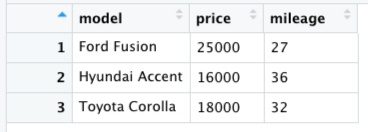
\includegraphics[width=5.11in]{images/cars_df} \caption{A view of the cars data frame generated by the View() function.}\label{fig:carsDf}
\end{figure}

Each of the columns in the data frame contains one of the variables, with the name that we gave it when we created the data frame. We can access each of those columns using the \texttt{\$} operator. For example, if we wanted to access the mileage variable, we would combine the name of the data frame with the name of the variable as follows:

\begin{verbatim}
> cars_df$mileage
[1] 27 36 32
\end{verbatim}

This is just like any other vector, in that we can refer to its individual values using square brackets as we did with regular vectors:

\begin{verbatim}
> cars_df$mileage[3]
[1] 32
\end{verbatim}

In some of the examples in the book, you will see something called a \emph{tibble}; this is basically a souped-up version of a data frame, and can be treated mostly in the same way.

\hypertarget{using-r-libraries}{%
\section{Using R libraries}\label{using-r-libraries}}

Many of the useful features in R are not contained in the primary R package, but instead come from \emph{libraries} that have been developed by various members of the R community. For example, the \texttt{ggplot2} package provides a number of features for visualizing data, as we will see in a later chapter. Before we can use a package, we need to install it on our system, using the \texttt{install.packages()} function:

\begin{verbatim}
> install.packages("ggplot2")
trying URL 'https://cran.rstudio.com/...
Content type 'application/x-gzip' length 3961383 bytes (3.8 MB)
==================================================
downloaded 3.8 MB


The downloaded binary packages are in
    /var/folders/.../downloaded_packages
\end{verbatim}

This will automatically download the package from the Comprehensive R Archive Network (CRAN) and install it on your system. Once it's installed, you can then load the library using the \texttt{library()} function:

\begin{verbatim}
> library(ggplot2)
\end{verbatim}

After loading the function, you can now access all of its features. If you want to learn more about its features, you can find them using the help function:

\begin{verbatim}
> help(ggplot2)
\end{verbatim}

\hypertarget{working-with-data-files}{%
\section{Working with data files}\label{working-with-data-files}}

When we are doing statistics, we often need to load in the data that we will analyze. Those data will live in a file on one's computer or on the internet. For this example, let's use a file that is hosted on the internet, which contains the gross domestic product (GDP) values for a number of countries around the world. This file is stored as \emph{comma-delimited text}, meaning that the values for each of the variables in the dataset are separate by commas. There are three variables: the relative rank of the countries, the name of the country, and its GDP value. Here is what the first few lines of the file look like:

\begin{verbatim}
Rank,Country,GDP
1,Liechtenstein,141100
2,Qatar,104300
3,Luxembourg,81100
\end{verbatim}

We can load a comma-delimited text file into R using the \texttt{read.csv()} function, which will accept either the location of a file on one's computer, or a URL for files that are located on the web:

\begin{verbatim}
url='https://raw.githubusercontent.com/psych10/
psych10/master/notebooks/Session03-IntroToR/gdp.csv'
gdp_df <- read.csv(url)
\end{verbatim}

Once you have done this, take a look at the data frame using the \texttt{View()} function, and make sure that it looks right --- it should have a column for each of the three variables.

Let's say that we wanted to create a new file, which contained GDP values in Euros rather than US Dollars. We use today's exchange rate, which is 1 USD == 0.90 Euros. To convert from Dollars to Euros, we simply multiple the GDP values by the exchange rate, and assign those values to a new variable within the data frame:

\begin{verbatim}
> exchange_rate = 0.9
> gdp_df$GDP_euros <- gdp_df$GDP * exchange_rate
\end{verbatim}

You should now see a new variable within the data frame, called ``GDP\_euros'' which contains the new values. Now let's save this to a comma-delimited text file on our computer called ``gdp\_euro.csv''.
We do this using the \texttt{write.table()} command.

\begin{verbatim}
> write.table(gdp_df, file='gdp_euro.csv')
\end{verbatim}

This file will be created with the working directory that RStudio is using. You can find this directory using the \texttt{getwd()} function:

\begin{verbatim}
> getwd()
[1] "/Users/me/MyClasses/Psych10/LearningR"
\end{verbatim}

\hypertarget{learning-objectives}{%
\section{Learning objectives}\label{learning-objectives}}

Having finished this chapter, you should be able to:

\begin{itemize}
\tightlist
\item
  Interact with an RMarkdown notebook in RStudio
\item
  Describe the difference between a variable and a function
\item
  Describe the different types of variables
\item
  Create a vector or data frame and access its elements
\item
  Install and load an R library
\item
  Load data from a file and view the data frame
\end{itemize}

\hypertarget{suggested-readings-and-videos}{%
\section{Suggested readings and videos}\label{suggested-readings-and-videos}}

There are many online resources for learning R. Here are a few:

\begin{itemize}
\tightlist
\item
  \href{https://www.datacamp.com/}{Datacamp}: Offers free online courses for many aspects of R programming
\item
  \href{https://cran.r-project.org/doc/contrib/Horton+Pruim+Kaplan_MOSAIC-StudentGuide.pdf}{A Student's Guide to R}
\item
  \href{https://rforcats.net/}{R for cats}: A humorous introduction to R programming
\item
  \href{http://arrgh.tim-smith.us/}{aRrgh: a newcomer's (angry) guide to R}
\item
  \href{http://www.statmethods.net/index.html}{Quick-R}
\item
  \href{https://www.rstudio.com/resources/cheatsheets/}{RStudio Cheat Sheets}: Quick references for many different aspects of R programming
\item
  \href{https://style.tidyverse.org/}{tidverse Style Guide}: Make your code beautiful and reader-friendly!
\item
  \href{http://r4ds.had.co.nz/index.html}{R for Data Science}: This free online book focuses on working with data in R.
\item
  \href{http://adv-r.had.co.nz/}{Advanced R}: This free online book by Hadley Wickham will help you get to the next level once your R skills start to develop.
\item
  \href{http://ramnathv.github.io/pycon2014-r/}{R intro for Python users}: Used Python before? Check this out for a guide on how to transition to R.
\end{itemize}

\hypertarget{summarizing-data-with-r-with-lucy-king}{%
\chapter{Summarizing data with R (with Lucy King)}\label{summarizing-data-with-r-with-lucy-king}}

This chapter will introduce you to how to summarize data using R, as well as providing an introduction to a popular set of R tools known as the ``Tidyverse.''

Before doing anything else we need to load the libraries that we will use in this notebook.

\begin{Shaded}
\begin{Highlighting}[]
\KeywordTok{library}\NormalTok{(tidyverse)}
\KeywordTok{library}\NormalTok{(cowplot)}
\KeywordTok{library}\NormalTok{(knitr)}
\KeywordTok{set.seed}\NormalTok{(}\DecValTok{123456}\NormalTok{)}
\NormalTok{opts_chunk}\OperatorTok{$}\KeywordTok{set}\NormalTok{(}\DataTypeTok{tidy.opts=}\KeywordTok{list}\NormalTok{(}\DataTypeTok{width.cutoff=}\DecValTok{80}\NormalTok{))}
\KeywordTok{options}\NormalTok{(}\DataTypeTok{tibble.width =} \DecValTok{60}\NormalTok{)}
\end{Highlighting}
\end{Shaded}

We will use the NHANES dataset for several of our examples, so let's load the library that contains the data.

\begin{Shaded}
\begin{Highlighting}[]
\CommentTok{# load the NHANES data library}
\CommentTok{# first unload it if it's already loaded, to make sure}
\CommentTok{# we have a clean version}
\KeywordTok{rm}\NormalTok{(}\StringTok{'NHANES'}\NormalTok{)}
\KeywordTok{library}\NormalTok{(NHANES)}
\KeywordTok{dim}\NormalTok{(NHANES)}
\end{Highlighting}
\end{Shaded}

\begin{verbatim}
## [1] 10000    76
\end{verbatim}

\hypertarget{introduction-to-the-tidyverse}{%
\section{Introduction to the Tidyverse}\label{introduction-to-the-tidyverse}}

In this chapter we will introduce a way of working with data in R that is often referred to as the ``Tidyverse.'' This comprises a set of packages that provide various tools for working with data, as well as a few special ways of using those functions

\hypertarget{making-a-data-frame-using-tibble}{%
\subsection{Making a data frame using tibble()}\label{making-a-data-frame-using-tibble}}

The tidyverse provides its own version of a data frame, which is known as a \emph{tibble}. A tibble is a data frame but with some smart tweaks that make it easier to work with, expecially when using functions from the tidyverse. See here for more information on the function \texttt{tibble()}: \url{https://r4ds.had.co.nz/tibbles.html}

\begin{Shaded}
\begin{Highlighting}[]
\CommentTok{# first create the individual variables}
\NormalTok{n <-}\StringTok{ }\KeywordTok{c}\NormalTok{(}\StringTok{"russ"}\NormalTok{, }\StringTok{"lucy"}\NormalTok{, }\StringTok{"jaclyn"}\NormalTok{, }\StringTok{"tyler"}\NormalTok{)}
\NormalTok{x <-}\StringTok{ }\KeywordTok{c}\NormalTok{(}\DecValTok{1}\NormalTok{, }\DecValTok{2}\NormalTok{, }\DecValTok{3}\NormalTok{, }\DecValTok{4}\NormalTok{)}
\NormalTok{y <-}\StringTok{ }\KeywordTok{c}\NormalTok{(}\DecValTok{4}\NormalTok{, }\DecValTok{5}\NormalTok{, }\DecValTok{6}\NormalTok{, }\DecValTok{7}\NormalTok{)}
\NormalTok{z <-}\StringTok{ }\KeywordTok{c}\NormalTok{(}\DecValTok{7}\NormalTok{, }\DecValTok{8}\NormalTok{, }\DecValTok{9}\NormalTok{, }\DecValTok{10}\NormalTok{)}

\CommentTok{# create the data frame}
\NormalTok{myDataFrame <-}
\StringTok{  }\KeywordTok{tibble}\NormalTok{(}
\NormalTok{    n, }\CommentTok{#list each of your columns in the order you want them}
\NormalTok{    x,}
\NormalTok{    y,}
\NormalTok{    z}
\NormalTok{  )}

\NormalTok{myDataFrame}
\end{Highlighting}
\end{Shaded}

\begin{verbatim}
## # A tibble: 4 x 4
##   n          x     y     z
##   <chr>  <dbl> <dbl> <dbl>
## 1 russ       1     4     7
## 2 lucy       2     5     8
## 3 jaclyn     3     6     9
## 4 tyler      4     7    10
\end{verbatim}

Take a quick look at the properties of the data frame using \texttt{glimpse()}:

\begin{Shaded}
\begin{Highlighting}[]
\KeywordTok{glimpse}\NormalTok{(myDataFrame) }
\end{Highlighting}
\end{Shaded}

\begin{verbatim}
## Observations: 4
## Variables: 4
## $ n <chr> "russ", "lucy", "jaclyn", "tyler"
## $ x <dbl> 1, 2, 3, 4
## $ y <dbl> 4, 5, 6, 7
## $ z <dbl> 7, 8, 9, 10
\end{verbatim}

\hypertarget{selecting-an-element}{%
\subsection{Selecting an element}\label{selecting-an-element}}

There are various ways to access the contents within a data frame.

\hypertarget{selecting-a-row-or-column-by-name}{%
\subsubsection{Selecting a row or column by name}\label{selecting-a-row-or-column-by-name}}

\begin{Shaded}
\begin{Highlighting}[]
\NormalTok{myDataFrame}\OperatorTok{$}\NormalTok{x}
\end{Highlighting}
\end{Shaded}

\begin{verbatim}
## [1] 1 2 3 4
\end{verbatim}

The first index refers to the row, the second to the column.

\begin{Shaded}
\begin{Highlighting}[]
\NormalTok{myDataFrame[}\DecValTok{1}\NormalTok{, }\DecValTok{2}\NormalTok{]}
\end{Highlighting}
\end{Shaded}

\begin{verbatim}
## # A tibble: 1 x 1
##       x
##   <dbl>
## 1     1
\end{verbatim}

\begin{Shaded}
\begin{Highlighting}[]
\NormalTok{myDataFrame[}\DecValTok{2}\NormalTok{, }\DecValTok{3}\NormalTok{]}
\end{Highlighting}
\end{Shaded}

\begin{verbatim}
## # A tibble: 1 x 1
##       y
##   <dbl>
## 1     5
\end{verbatim}

\hypertarget{selecting-a-row-or-column-by-index}{%
\subsubsection{Selecting a row or column by index}\label{selecting-a-row-or-column-by-index}}

\begin{Shaded}
\begin{Highlighting}[]
\NormalTok{myDataFrame[}\DecValTok{1}\NormalTok{, ]}
\end{Highlighting}
\end{Shaded}

\begin{verbatim}
## # A tibble: 1 x 4
##   n         x     y     z
##   <chr> <dbl> <dbl> <dbl>
## 1 russ      1     4     7
\end{verbatim}

\begin{Shaded}
\begin{Highlighting}[]
\NormalTok{myDataFrame[, }\DecValTok{1}\NormalTok{]}
\end{Highlighting}
\end{Shaded}

\begin{verbatim}
## # A tibble: 4 x 1
##   n     
##   <chr> 
## 1 russ  
## 2 lucy  
## 3 jaclyn
## 4 tyler
\end{verbatim}

\hypertarget{select-a-set-of-rows}{%
\subsubsection{Select a set of rows}\label{select-a-set-of-rows}}

\begin{Shaded}
\begin{Highlighting}[]
\NormalTok{myDataFrame }\OperatorTok\StringTok{ }
\StringTok{  }\KeywordTok{slice}\NormalTok{(}\DecValTok{1}\OperatorTok{:}\DecValTok{2}\NormalTok{) }
\end{Highlighting}
\end{Shaded}

\begin{verbatim}
## # A tibble: 2 x 4
##   n         x     y     z
##   <chr> <dbl> <dbl> <dbl>
## 1 russ      1     4     7
## 2 lucy      2     5     8
\end{verbatim}

\texttt{slice()} is a function that selects out rows based on their row number.

You will also notice something we haven't discussed before: \texttt{\%\textgreater{}\%}. This is called a ``pipe'', which is commonly used within the tidyverse; you can read more \href{http://magrittr.tidyverse.org/}{here}. A pipe takes the output from one command and feeds it as input to the next command. In this case, simply writing the name of the data frame (myDataFrame) causes it to be input to the \texttt{slice()} command following the pipe. The benefit of pipes will become especially apparent when we want to start stringing together multiple data processing operations into a single command.

In the previous example, no new variable was created - the output was simply printed to the screen, just like it would be if you typed the name of the variable. If you wanted to save it to a new variable, you would use the \texttt{\textless{}-} assignment operator, like this:

\begin{Shaded}
\begin{Highlighting}[]
\NormalTok{myDataFrameSlice <-}\StringTok{ }\NormalTok{myDataFrame }\OperatorTok\StringTok{ }
\StringTok{  }\KeywordTok{slice}\NormalTok{(}\DecValTok{1}\OperatorTok{:}\DecValTok{2}\NormalTok{) }

\NormalTok{myDataFrameSlice}
\end{Highlighting}
\end{Shaded}

\begin{verbatim}
## # A tibble: 2 x 4
##   n         x     y     z
##   <chr> <dbl> <dbl> <dbl>
## 1 russ      1     4     7
## 2 lucy      2     5     8
\end{verbatim}

\hypertarget{select-a-set-of-rows-based-on-specific-values}{%
\subsubsection{Select a set of rows based on specific value(s)}\label{select-a-set-of-rows-based-on-specific-values}}

\begin{Shaded}
\begin{Highlighting}[]
\NormalTok{myDataFrame }\OperatorTok\StringTok{ }
\StringTok{  }\KeywordTok{filter}\NormalTok{(n }\OperatorTok{==}\StringTok{ "russ"}\NormalTok{)}
\end{Highlighting}
\end{Shaded}

\begin{verbatim}
## # A tibble: 1 x 4
##   n         x     y     z
##   <chr> <dbl> <dbl> <dbl>
## 1 russ      1     4     7
\end{verbatim}

\texttt{filter()} is a function that retains only those rows that meet your stated criteria. We can also filter for multiple criteria at once --- in this example, the \texttt{\textbar{}} symbol indicates ``or'':

\begin{Shaded}
\begin{Highlighting}[]
\NormalTok{myDataFrame }\OperatorTok\StringTok{ }
\StringTok{  }\KeywordTok{filter}\NormalTok{(n }\OperatorTok{==}\StringTok{ "russ"} \OperatorTok{|}\StringTok{ }\NormalTok{n }\OperatorTok{==}\StringTok{ "lucy"}\NormalTok{)}
\end{Highlighting}
\end{Shaded}

\begin{verbatim}
## # A tibble: 2 x 4
##   n         x     y     z
##   <chr> <dbl> <dbl> <dbl>
## 1 russ      1     4     7
## 2 lucy      2     5     8
\end{verbatim}

\hypertarget{select-a-set-of-columns}{%
\subsubsection{Select a set of columns}\label{select-a-set-of-columns}}

\begin{Shaded}
\begin{Highlighting}[]
\NormalTok{myDataFrame }\OperatorTok\StringTok{ }
\StringTok{  }\KeywordTok{select}\NormalTok{(x}\OperatorTok{:}\NormalTok{y)}
\end{Highlighting}
\end{Shaded}

\begin{verbatim}
## # A tibble: 4 x 2
##       x     y
##   <dbl> <dbl>
## 1     1     4
## 2     2     5
## 3     3     6
## 4     4     7
\end{verbatim}

\texttt{select()} is a function that selects out only those columns you specify using their names

You can also specify a vector of columns to select.

\begin{Shaded}
\begin{Highlighting}[]
\NormalTok{myDataFrame }\OperatorTok\StringTok{ }
\StringTok{  }\KeywordTok{select}\NormalTok{(}\KeywordTok{c}\NormalTok{(x,z))}
\end{Highlighting}
\end{Shaded}

\begin{verbatim}
## # A tibble: 4 x 2
##       x     z
##   <dbl> <dbl>
## 1     1     7
## 2     2     8
## 3     3     9
## 4     4    10
\end{verbatim}

\hypertarget{adding-a-row-or-column}{%
\subsection{Adding a row or column}\label{adding-a-row-or-column}}

add a named row

\begin{Shaded}
\begin{Highlighting}[]
\NormalTok{tiffanyDataFrame <-}
\StringTok{  }\KeywordTok{tibble}\NormalTok{(}
    \DataTypeTok{n =} \StringTok{"tiffany"}\NormalTok{,}
    \DataTypeTok{x =} \DecValTok{13}\NormalTok{,}
    \DataTypeTok{y =} \DecValTok{14}\NormalTok{,}
    \DataTypeTok{z =} \DecValTok{15}
\NormalTok{  )}

\NormalTok{myDataFrame }\OperatorTok\StringTok{ }
\StringTok{  }\KeywordTok{bind_rows}\NormalTok{(tiffanyDataFrame)}
\end{Highlighting}
\end{Shaded}

\begin{verbatim}
## # A tibble: 5 x 4
##   n           x     y     z
##   <chr>   <dbl> <dbl> <dbl>
## 1 russ        1     4     7
## 2 lucy        2     5     8
## 3 jaclyn      3     6     9
## 4 tyler       4     7    10
## 5 tiffany    13    14    15
\end{verbatim}

\texttt{bind\_rows()} is a function that combines the rows from another dataframe to the current dataframe

\hypertarget{creating-or-modifying-variables-using-mutate}{%
\section{\texorpdfstring{Creating or modifying variables using \texttt{mutate()}}{Creating or modifying variables using mutate()}}\label{creating-or-modifying-variables-using-mutate}}

Often we will want to either create a new variable based on an existing variable, or modify the value of an existing variable. Within the tidyverse, we do this using a function called \texttt{mutate()}. Let's start with a toy example by creating a data frame containing a single variable.

\begin{Shaded}
\begin{Highlighting}[]
\NormalTok{toy_df <-}\StringTok{ }\KeywordTok{data.frame}\NormalTok{(}\DataTypeTok{x =} \KeywordTok{c}\NormalTok{(}\DecValTok{1}\NormalTok{,}\DecValTok{2}\NormalTok{,}\DecValTok{3}\NormalTok{,}\DecValTok{4}\NormalTok{))}
\KeywordTok{glimpse}\NormalTok{(toy_df)}
\end{Highlighting}
\end{Shaded}

\begin{verbatim}
## Observations: 4
## Variables: 1
## $ x <dbl> 1, 2, 3, 4
\end{verbatim}

Let's say that we wanted to create a new variable called \texttt{y} that would contain the value of x multiplied by 10. We could do this using \texttt{mutate()} and then assign the result back to the same data frame:

\begin{Shaded}
\begin{Highlighting}[]
\NormalTok{toy_df <-}\StringTok{ }\NormalTok{toy_df }\OperatorTok
\StringTok{  }\CommentTok{# create a new variable called y that contains x*10}
\StringTok{  }\KeywordTok{mutate}\NormalTok{(}\DataTypeTok{y =}\NormalTok{ x}\OperatorTok{*}\DecValTok{10}\NormalTok{)}
\KeywordTok{glimpse}\NormalTok{(toy_df)}
\end{Highlighting}
\end{Shaded}

\begin{verbatim}
## Observations: 4
## Variables: 2
## $ x <dbl> 1, 2, 3, 4
## $ y <dbl> 10, 20, 30, 40
\end{verbatim}

We could also overwrite a variable with a new value:

\begin{Shaded}
\begin{Highlighting}[]
\NormalTok{toy_df2 <-}\StringTok{ }\NormalTok{toy_df }\OperatorTok
\StringTok{  }\CommentTok{# create a new variable called y that contains x*10}
\StringTok{  }\KeywordTok{mutate}\NormalTok{(}\DataTypeTok{y =}\NormalTok{ y }\OperatorTok{+}\StringTok{ }\DecValTok{1}\NormalTok{)}
\KeywordTok{glimpse}\NormalTok{(toy_df2)}
\end{Highlighting}
\end{Shaded}

\begin{verbatim}
## Observations: 4
## Variables: 2
## $ x <dbl> 1, 2, 3, 4
## $ y <dbl> 11, 21, 31, 41
\end{verbatim}

We will use \texttt{mutate()} often so it's an important function to understand.

Here we can use it with our example data frame to create a new variable that is the sum of several other variables.

\begin{Shaded}
\begin{Highlighting}[]
\NormalTok{myDataFrame <-}\StringTok{ }
\StringTok{  }\NormalTok{myDataFrame }\OperatorTok
\StringTok{  }\KeywordTok{mutate}\NormalTok{(}\DataTypeTok{total =}\NormalTok{ x }\OperatorTok{+}\StringTok{ }\NormalTok{y }\OperatorTok{+}\StringTok{ }\NormalTok{z)}

\KeywordTok{kable}\NormalTok{(myDataFrame)}
\end{Highlighting}
\end{Shaded}

\begin{tabular}{l|r|r|r|r}
\hline
n & x & y & z & total\\
\hline
russ & 1 & 4 & 7 & 12\\
\hline
lucy & 2 & 5 & 8 & 15\\
\hline
jaclyn & 3 & 6 & 9 & 18\\
\hline
tyler & 4 & 7 & 10 & 21\\
\hline
\end{tabular}

mutate() is a function that creates a new variable in a data frame using the existing variables. In this case, it creates a variable called total that is the sum of the existing variables x, y, and z.

\hypertarget{remove-a-column-using-the-select-function}{%
\subsection{Remove a column using the select() function}\label{remove-a-column-using-the-select-function}}

Adding a minus sign to the name of a variable within the \texttt{select()} command will remove that variable, leaving all of the others.

\begin{Shaded}
\begin{Highlighting}[]
\NormalTok{myDataFrame <-}\StringTok{ }
\StringTok{  }\NormalTok{myDataFrame }\OperatorTok
\StringTok{  }\NormalTok{dplyr}\OperatorTok{::}\KeywordTok{select}\NormalTok{(}\OperatorTok{-}\NormalTok{total)}

\KeywordTok{kable}\NormalTok{(myDataFrame)}
\end{Highlighting}
\end{Shaded}

\begin{tabular}{l|r|r|r}
\hline
n & x & y & z\\
\hline
russ & 1 & 4 & 7\\
\hline
lucy & 2 & 5 & 8\\
\hline
jaclyn & 3 & 6 & 9\\
\hline
tyler & 4 & 7 & 10\\
\hline
\end{tabular}

\hypertarget{tidyverse-in-action}{%
\section{Tidyverse in action}\label{tidyverse-in-action}}

To see the tidyverse in action, let's clean up the NHANES dataset. Each individual in the NHANES dataset has a unique identifier stored in the variable \texttt{ID}. First let's look at the number of rows in the dataset:

\begin{Shaded}
\begin{Highlighting}[]
\KeywordTok{nrow}\NormalTok{(NHANES)}
\end{Highlighting}
\end{Shaded}

\begin{verbatim}
## [1] 10000
\end{verbatim}

Now let's see how many unique IDs there are. The \texttt{unique()} function returns a vector containing all of the unique values for a particular variable, and the \texttt{length()} function returns the length of the resulting vector.

\begin{Shaded}
\begin{Highlighting}[]
\KeywordTok{length}\NormalTok{(}\KeywordTok{unique}\NormalTok{(NHANES}\OperatorTok{$}\NormalTok{ID))}
\end{Highlighting}
\end{Shaded}

\begin{verbatim}
## [1] 6779
\end{verbatim}

This shows us that while there are 10,000 observations in the data frame, there are only 6779 unique IDs. This means that if we were to use the entire dataset, we would be reusing data from some individuals, which could give us incorrect results. For this reason, we wold like to discard any observations that are duplicated.

Let's create a new variable called \texttt{NHANES\_unique} that will contain only the distinct observations, with no individuals appearing more than once. The \texttt{dplyr} library provides a function called \texttt{distinct()} that will do this for us. You may notice that we didn't explicitly load the \texttt{dplyr} library above; however, if you look at the messages that appeared when we loaded the \texttt{tidyverse} library, you will see that it loaded \texttt{dplyr} for us. To create the new data frame with unique observations, we will pipe the NHANES data frame into the \texttt{distinct()} function and then save the output to our new variable.

\begin{Shaded}
\begin{Highlighting}[]
\NormalTok{NHANES_unique <-}\StringTok{ }
\StringTok{  }\NormalTok{NHANES }\OperatorTok\StringTok{ }
\StringTok{  }\KeywordTok{distinct}\NormalTok{(ID, }\DataTypeTok{.keep_all =} \OtherTok{TRUE}\NormalTok{)}
\end{Highlighting}
\end{Shaded}

If we number of rows in the new data frame, it should be the same as the number of unique IDs (6779):

\begin{Shaded}
\begin{Highlighting}[]
\KeywordTok{nrow}\NormalTok{(NHANES_unique)}
\end{Highlighting}
\end{Shaded}

\begin{verbatim}
## [1] 6779
\end{verbatim}

In the next example you will see the power of pipes come to life, when we start tying together multiple functions into a single operation (or ``pipeline'').

\hypertarget{looking-at-individual-variables-using-pull-and-head}{%
\section{Looking at individual variables using pull() and head()}\label{looking-at-individual-variables-using-pull-and-head}}

The NHANES data frame contains a large number of variables, but usually we are only interested in a particular variable. We can extract a particular variable from a data frame using the \texttt{pull()} function. Let's say that we want to extract the variable \texttt{PhysActive}. We could do this by piping the data frame into the pull command, which will result in a list of many thousands of values. Instead of printing out this entire list, we will pipe the result into the \texttt{head()} function, which just shows us the first few values contained in a variable. In this case we are not assigning the value back to a variable, so it will simply be printed to the screen.

\begin{Shaded}
\begin{Highlighting}[]
\NormalTok{NHANES }\OperatorTok
\StringTok{  }\CommentTok{# extract the PhysActive variable}
\StringTok{  }\KeywordTok{pull}\NormalTok{(PhysActive) }\OperatorTok
\StringTok{  }\CommentTok{# extract the first 10 values }
\StringTok{  }\KeywordTok{head}\NormalTok{(}\DecValTok{10}\NormalTok{) }\OperatorTok
\StringTok{  }\KeywordTok{kable}\NormalTok{()}
\end{Highlighting}
\end{Shaded}

\begin{tabular}{l}
\hline
x\\
\hline
No\\
\hline
No\\
\hline
No\\
\hline
NA\\
\hline
No\\
\hline
NA\\
\hline
NA\\
\hline
Yes\\
\hline
Yes\\
\hline
Yes\\
\hline
\end{tabular}

There are two important things to notice here. The first is that there are three different values apparent in the answers: ``Yes'', ``No'', and , which means that the value is missing for this person (perhaps they didn't want to answer that question on the survey). When we are working with data we generally need to remove missing values, as we will see below.

The second thing to notice is that R prints out a list of ``Levels'' of the variable. This is because this variable is defined as a particular kind of variable in R known as a \emph{factor}. You can think of a factor variable as a categorial variable with a specific set of levels. The missing data are not treated as a level, so it can be useful to make the missing values explicit, which can be done using a function called \texttt{fct\_explicit\_na()} in the \texttt{forcats} package. Let's add a line to do that:

\begin{Shaded}
\begin{Highlighting}[]
\NormalTok{NHANES }\OperatorTok
\StringTok{  }\KeywordTok{mutate}\NormalTok{(}\DataTypeTok{PhysActive =} \KeywordTok{fct_explicit_na}\NormalTok{(PhysActive)) }\OperatorTok
\StringTok{  }\CommentTok{# extract the PhysActive variable}
\StringTok{  }\KeywordTok{pull}\NormalTok{(PhysActive) }\OperatorTok
\StringTok{  }\CommentTok{# extract the first 10 values }
\StringTok{  }\KeywordTok{head}\NormalTok{(}\DecValTok{10}\NormalTok{) }\OperatorTok
\StringTok{  }\KeywordTok{kable}\NormalTok{()}
\end{Highlighting}
\end{Shaded}

\begin{tabular}{l}
\hline
x\\
\hline
No\\
\hline
No\\
\hline
No\\
\hline
(Missing)\\
\hline
No\\
\hline
(Missing)\\
\hline
(Missing)\\
\hline
Yes\\
\hline
Yes\\
\hline
Yes\\
\hline
\end{tabular}

This new line overwrote the old value of \texttt{PhysActive} with a version that has been processed by the \texttt{fct\_explicit\_na()} function to convert values to explicitly missing values. Now you can see that Missing values are treated as an explicit level, which will be useful later.

Now we are ready to start summarizing data!

\hypertarget{computing-a-frequency-distribution-section-reffrequency-distributions}{%
\section{Computing a frequency distribution (Section \ref{frequency-distributions})}\label{computing-a-frequency-distribution-section-reffrequency-distributions}}

We would like to compute a frequency distribution showing how many people report being either active or inactive. The following statement is fairly complex so we will step through it one bit at a time.

\begin{Shaded}
\begin{Highlighting}[]
\NormalTok{PhysActive_table <-}\StringTok{ }\NormalTok{NHANES_unique }\OperatorTok
\StringTok{  }\CommentTok{# convert the implicit missing values to explicit}
\StringTok{  }\KeywordTok{mutate}\NormalTok{(}\DataTypeTok{PhysActive =} \KeywordTok{fct_explicit_na}\NormalTok{(PhysActive)) }\OperatorTok
\StringTok{  }\CommentTok{# select the variable of interest}
\StringTok{  }\NormalTok{dplyr}\OperatorTok{::}\KeywordTok{select}\NormalTok{(PhysActive) }\OperatorTok\StringTok{ }
\StringTok{  }\CommentTok{# group by values of the variable}
\StringTok{  }\KeywordTok{group_by}\NormalTok{(PhysActive) }\OperatorTok\StringTok{ }
\StringTok{  }\CommentTok{# count the values}
\StringTok{  }\KeywordTok{summarize}\NormalTok{(}\DataTypeTok{AbsoluteFrequency =} \KeywordTok{n}\NormalTok{()) }

\CommentTok{# kable() prints out the table in a prettier way.}
\KeywordTok{kable}\NormalTok{(PhysActive_table)}
\end{Highlighting}
\end{Shaded}

\begin{tabular}{l|r}
\hline
PhysActive & AbsoluteFrequency\\
\hline
No & 2473\\
\hline
Yes & 2972\\
\hline
(Missing) & 1334\\
\hline
\end{tabular}

This data frame still contains all of the original variables. Since we are only interested in the \texttt{PhysActive} variable, let's extract that one and get rid of the rest. We can do this using the \texttt{select()} command from the \texttt{dplyr} package. Because there is also another select command available in R, we need to explicitly refer to the one from the \texttt{dplyr} package, which we do by including the package name followed by two colons: \texttt{dplyr::select()}.

\begin{Shaded}
\begin{Highlighting}[]
\NormalTok{NHANES_unique }\OperatorTok
\StringTok{  }\CommentTok{# convert the implicit missing values to explicit}
\StringTok{  }\KeywordTok{mutate}\NormalTok{(}\DataTypeTok{PhysActive =} \KeywordTok{fct_explicit_na}\NormalTok{(PhysActive)) }\OperatorTok
\StringTok{  }\CommentTok{# select the variable of interest}
\StringTok{  }\NormalTok{dplyr}\OperatorTok{::}\KeywordTok{select}\NormalTok{(PhysActive) }\OperatorTok\StringTok{ }
\StringTok{  }\KeywordTok{head}\NormalTok{(}\DecValTok{10}\NormalTok{) }\OperatorTok
\StringTok{  }\KeywordTok{kable}\NormalTok{()}
\end{Highlighting}
\end{Shaded}

\begin{tabular}{l}
\hline
PhysActive\\
\hline
No\\
\hline
(Missing)\\
\hline
No\\
\hline
(Missing)\\
\hline
(Missing)\\
\hline
Yes\\
\hline
Yes\\
\hline
Yes\\
\hline
Yes\\
\hline
(Missing)\\
\hline
\end{tabular}

The next function, \texttt{group\_by()} tells R that we are going to want to analyze the data separate according to the different levels of the \texttt{PhysActive} variable:

\begin{Shaded}
\begin{Highlighting}[]
\NormalTok{NHANES_unique }\OperatorTok
\StringTok{  }\CommentTok{# convert the implicit missing values to explicit}
\StringTok{  }\KeywordTok{mutate}\NormalTok{(}\DataTypeTok{PhysActive =} \KeywordTok{fct_explicit_na}\NormalTok{(PhysActive)) }\OperatorTok
\StringTok{  }\CommentTok{# select the variable of interest}
\StringTok{  }\NormalTok{dplyr}\OperatorTok{::}\KeywordTok{select}\NormalTok{(PhysActive) }\OperatorTok\StringTok{ }
\StringTok{  }\KeywordTok{group_by}\NormalTok{(PhysActive) }\OperatorTok
\StringTok{  }\KeywordTok{head}\NormalTok{(}\DecValTok{10}\NormalTok{) }\OperatorTok
\StringTok{  }\KeywordTok{kable}\NormalTok{()}
\end{Highlighting}
\end{Shaded}

\begin{tabular}{l}
\hline
PhysActive\\
\hline
No\\
\hline
(Missing)\\
\hline
No\\
\hline
(Missing)\\
\hline
(Missing)\\
\hline
Yes\\
\hline
Yes\\
\hline
Yes\\
\hline
Yes\\
\hline
(Missing)\\
\hline
\end{tabular}

The final command tells R to create a new data frame by summarizing the data that we are passing in (which in this case is the PhysActive variable, grouped by its different levels). We tell the \texttt{summarize()} function to create a new variable (called \texttt{AbsoluteFrequency}) will contain a count of the number of observations for each group, which is generated by the \texttt{n()} function.

\begin{Shaded}
\begin{Highlighting}[]
\NormalTok{NHANES_unique }\OperatorTok
\StringTok{  }\CommentTok{# convert the implicit missing values to explicit}
\StringTok{  }\KeywordTok{mutate}\NormalTok{(}\DataTypeTok{PhysActive =} \KeywordTok{fct_explicit_na}\NormalTok{(PhysActive)) }\OperatorTok
\StringTok{  }\CommentTok{# select the variable of interest}
\StringTok{  }\NormalTok{dplyr}\OperatorTok{::}\KeywordTok{select}\NormalTok{(PhysActive) }\OperatorTok\StringTok{ }
\StringTok{  }\KeywordTok{group_by}\NormalTok{(PhysActive) }\OperatorTok
\StringTok{  }\KeywordTok{summarize}\NormalTok{(}\DataTypeTok{AbsoluteFrequency =} \KeywordTok{n}\NormalTok{())  }\OperatorTok
\StringTok{  }\KeywordTok{kable}\NormalTok{()}
\end{Highlighting}
\end{Shaded}

\begin{tabular}{l|r}
\hline
PhysActive & AbsoluteFrequency\\
\hline
No & 2473\\
\hline
Yes & 2972\\
\hline
(Missing) & 1334\\
\hline
\end{tabular}

Now let's say we want to add another column with percentage of observations in each group. We compute the percentage by dividing the absolute frequency for each group by the total number. We can use the table that we already generated, and add a new variable, again using \texttt{mutate()}:

\begin{Shaded}
\begin{Highlighting}[]
\NormalTok{PhysActive_table <-}\StringTok{ }\NormalTok{PhysActive_table }\OperatorTok
\StringTok{  }\KeywordTok{mutate}\NormalTok{(}
    \DataTypeTok{Percentage =}\NormalTok{ AbsoluteFrequency }\OperatorTok{/}\StringTok{ }
\StringTok{      }\KeywordTok{sum}\NormalTok{(AbsoluteFrequency) }\OperatorTok{*}\StringTok{ }\DecValTok{100}
\NormalTok{  )}

\KeywordTok{kable}\NormalTok{(PhysActive_table, }\DataTypeTok{digits=}\DecValTok{2}\NormalTok{)}
\end{Highlighting}
\end{Shaded}

\begin{tabular}{l|r|r}
\hline
PhysActive & AbsoluteFrequency & Percentage\\
\hline
No & 2473 & 36.48\\
\hline
Yes & 2972 & 43.84\\
\hline
(Missing) & 1334 & 19.68\\
\hline
\end{tabular}

\hypertarget{computing-a-cumulative-distribution-section-refcumulative-distributions}{%
\section{Computing a cumulative distribution (Section \ref{cumulative-distributions})}\label{computing-a-cumulative-distribution-section-refcumulative-distributions}}

Let's compute a cumulative distribution for the \texttt{SleepHrsNight} variable in NHANES. This looks very similar to what we saw in the previous section.

\begin{Shaded}
\begin{Highlighting}[]
\CommentTok{# create summary table for relative frequency of different}
\CommentTok{# values of SleepHrsNight }

\NormalTok{SleepHrsNight_cumulative <-}\StringTok{ }
\StringTok{  }\NormalTok{NHANES_unique }\OperatorTok
\StringTok{  }\CommentTok{# drop NA values for SleepHrsNight variable}
\StringTok{  }\KeywordTok{drop_na}\NormalTok{(SleepHrsNight) }\OperatorTok
\StringTok{  }\CommentTok{# remove other variables}
\StringTok{  }\NormalTok{dplyr}\OperatorTok{::}\KeywordTok{select}\NormalTok{(SleepHrsNight) }\OperatorTok
\StringTok{  }\CommentTok{# group by values}
\StringTok{  }\KeywordTok{group_by}\NormalTok{(SleepHrsNight) }\OperatorTok
\StringTok{  }\CommentTok{# create summary table}
\StringTok{  }\KeywordTok{summarize}\NormalTok{(}\DataTypeTok{AbsoluteFrequency =} \KeywordTok{n}\NormalTok{()) }\OperatorTok
\StringTok{  }\CommentTok{# create relative and cumulative frequencies}
\StringTok{  }\KeywordTok{mutate}\NormalTok{(}
    \DataTypeTok{RelativeFrequency =}\NormalTok{ AbsoluteFrequency }\OperatorTok{/}\StringTok{ }
\StringTok{      }\KeywordTok{sum}\NormalTok{(AbsoluteFrequency),}
    \DataTypeTok{CumulativeDensity =} \KeywordTok{cumsum}\NormalTok{(RelativeFrequency)}
\NormalTok{  )}

\KeywordTok{kable}\NormalTok{(SleepHrsNight_cumulative)}
\end{Highlighting}
\end{Shaded}

\begin{tabular}{r|r|r|r}
\hline
SleepHrsNight & AbsoluteFrequency & RelativeFrequency & CumulativeDensity\\
\hline
2 & 9 & 0.0017875 & 0.0017875\\
\hline
3 & 49 & 0.0097319 & 0.0115194\\
\hline
4 & 200 & 0.0397219 & 0.0512413\\
\hline
5 & 406 & 0.0806356 & 0.1318769\\
\hline
6 & 1172 & 0.2327706 & 0.3646475\\
\hline
7 & 1394 & 0.2768620 & 0.6415094\\
\hline
8 & 1405 & 0.2790467 & 0.9205561\\
\hline
9 & 271 & 0.0538232 & 0.9743793\\
\hline
10 & 97 & 0.0192651 & 0.9936445\\
\hline
11 & 15 & 0.0029791 & 0.9966236\\
\hline
12 & 17 & 0.0033764 & 1.0000000\\
\hline
\end{tabular}

\hypertarget{data-cleaning-and-tidying-with-r}{%
\section{Data cleaning and tidying with R}\label{data-cleaning-and-tidying-with-r}}

Now that you know a bit about the tidyverse, let's look at the various tools that it provides for working with data. We will use as an example an analysis of whether attitudes about statistics are different between the different student year groups in the class.

\hypertarget{statistics-attitude-data-from-course-survey}{%
\subsection{Statistics attitude data from course survey}\label{statistics-attitude-data-from-course-survey}}

These data were collected using the Attitudes Towards Statistics (ATS) scale (from \url{https://www.stat.auckland.ac.nz/~iase/cblumberg/wise2.pdf}).

The 29-item ATS has two subscales. The Attitudes Toward Field subscale consists of the following 20 items, with reverse-keyed items indicated by an ``(R)'':
1, 3, 5, 6(R), 9, 10(R), 11, 13, 14(R), 16(R), 17, 19, 20(R), 21, 22, 23, 24, 26, 28(R), 29

The Attitudes Toward Course subscale consists of the following 9 items:
2(R), 4(R), 7(R), 8, 12(R), 15(R), 18(R), 25(R), 27(R)

For our purposes, we will just combine all 29 items together, rather than separating them into these subscales.

Note: I have removed the data from the graduate students and 5+ year students, since those would be too easily identifiable given how few there are.

Let's first save the file path to the data.

\begin{Shaded}
\begin{Highlighting}[]
\NormalTok{attitudeData_file <-}\StringTok{ 'data/statsAttitude.txt'}
\end{Highlighting}
\end{Shaded}

Next, let's load the data from the file using the tidyverse function \texttt{read\_tsv()}. There are several functions available for reading in different file formats as part of the the \texttt{readr} tidyverse package.

Right now the variable names are unwieldy, since they include the entire name of the item; this is how Google Forms stores the data. Let's change the variable names to be somewhat more readable. We will change the names to ``ats'' where is replaced with the question number and ats indicates Attitudes Toward Statistics scale. We can create these names using the \texttt{rename()} and \texttt{paste0()} functions. \texttt{rename()} is pretty self-explanatory: a new name is assigned to an old name or a column position. The \texttt{paste0()} function takes a string along with a set of numbers, and creates a vector that combines the string with the number.

\begin{Shaded}
\begin{Highlighting}[]
\NormalTok{nQuestions <-}\StringTok{ }\DecValTok{29} \CommentTok{# other than the first two columns, }
\CommentTok{# the rest of the columns are for the 29 questions in the statistics}
\CommentTok{# attitude survey; we'll use this below to rename these columns }
\CommentTok{# based on their question number}

\CommentTok{# use rename to change the first two column names}
\CommentTok{# rename can refer to columns either by their number or their name}
\NormalTok{attitudeData <-}
\StringTok{  }\NormalTok{attitudeData }\OperatorTok\StringTok{ }
\StringTok{  }\KeywordTok{rename}\NormalTok{(     }\CommentTok{# rename using columm numbers}
    \CommentTok{# The first column is the year }
    \DataTypeTok{Year =} \DecValTok{1}\NormalTok{, }
    \CommentTok{# The second column indicates }
    \CommentTok{# whether the person took stats before}
    \DataTypeTok{StatsBefore =} \DecValTok{2} 
\NormalTok{  ) }\OperatorTok\StringTok{ }
\StringTok{  }\KeywordTok{rename_at}\NormalTok{( }
    \CommentTok{# rename all the columns except Year and StatsBefore}
    \KeywordTok{vars}\NormalTok{(}\OperatorTok{-}\NormalTok{Year, }\OperatorTok{-}\NormalTok{StatsBefore), }
    \CommentTok{#rename by pasting the word "stat" and the number}
    \KeywordTok{list}\NormalTok{(}\DataTypeTok{name =} \OperatorTok{~}\KeywordTok{paste0}\NormalTok{(}\StringTok{'ats'}\NormalTok{, }\DecValTok{1}\OperatorTok{:}\NormalTok{nQuestions)) }
\NormalTok{  )}

\CommentTok{# print out the column names}
\KeywordTok{names}\NormalTok{(attitudeData)}
\end{Highlighting}
\end{Shaded}

\begin{verbatim}
##  [1] "Year"        "StatsBefore" "ats1"        "ats2"        "ats3"       
##  [6] "ats4"        "ats5"        "ats6"        "ats7"        "ats8"       
## [11] "ats9"        "ats10"       "ats11"       "ats12"       "ats13"      
## [16] "ats14"       "ats15"       "ats16"       "ats17"       "ats18"      
## [21] "ats19"       "ats20"       "ats21"       "ats22"       "ats23"      
## [26] "ats24"       "ats25"       "ats26"       "ats27"       "ats28"      
## [31] "ats29"
\end{verbatim}

\begin{Shaded}
\begin{Highlighting}[]
\CommentTok{#check out the data again}
\KeywordTok{glimpse}\NormalTok{(attitudeData)}
\end{Highlighting}
\end{Shaded}

\begin{verbatim}
## Observations: 148
## Variables: 31
## $ Year        <dbl> 3, 4, 2, 1, 2, 3, 4, 2, 2, 2, 4, 2,...
## $ StatsBefore <chr> "Yes", "No", "No", "Yes", "No", "No...
## $ ats1        <dbl> 6, 4, 6, 3, 7, 4, 6, 5, 7, 5, 5, 4,...
## $ ats2        <dbl> 1, 5, 5, 2, 7, 5, 5, 4, 2, 2, 3, 3,...
## $ ats3        <dbl> 7, 6, 5, 7, 2, 4, 7, 7, 7, 5, 6, 5,...
## $ ats4        <dbl> 2, 5, 5, 2, 7, 3, 3, 4, 5, 3, 3, 2,...
## $ ats5        <dbl> 7, 5, 6, 7, 5, 4, 6, 6, 7, 5, 3, 5,...
## $ ats6        <dbl> 1, 4, 5, 2, 2, 4, 2, 3, 1, 2, 2, 3,...
## $ ats7        <dbl> 1, 4, 3, 2, 4, 4, 2, 2, 3, 2, 4, 2,...
## $ ats8        <dbl> 2, 1, 4, 3, 1, 4, 4, 4, 7, 3, 2, 4,...
## $ ats9        <dbl> 5, 4, 5, 5, 7, 4, 5, 5, 7, 6, 3, 5,...
## $ ats10       <dbl> 2, 3, 2, 2, 1, 4, 2, 2, 1, 3, 3, 1,...
## $ ats11       <dbl> 6, 4, 6, 2, 7, 4, 6, 5, 7, 3, 3, 4,...
## $ ats12       <dbl> 2, 4, 1, 2, 5, 7, 2, 1, 2, 4, 4, 2,...
## $ ats13       <dbl> 6, 4, 5, 5, 7, 3, 6, 6, 7, 5, 2, 5,...
## $ ats14       <dbl> 2, 4, 3, 3, 3, 4, 2, 1, 1, 3, 3, 2,...
## $ ats15       <dbl> 2, 4, 3, 3, 5, 6, 3, 4, 2, 3, 2, 4,...
## $ ats16       <dbl> 1, 3, 2, 5, 1, 5, 2, 1, 2, 3, 2, 2,...
## $ ats17       <dbl> 7, 7, 5, 7, 7, 4, 6, 6, 7, 6, 6, 7,...
## $ ats18       <dbl> 2, 5, 4, 5, 7, 4, 2, 4, 2, 5, 2, 4,...
## $ ats19       <dbl> 3, 3, 4, 3, 2, 3, 6, 5, 7, 3, 3, 5,...
## $ ats20       <dbl> 1, 4, 1, 2, 1, 4, 2, 2, 1, 2, 3, 2,...
## $ ats21       <dbl> 6, 3, 5, 5, 7, 5, 6, 5, 7, 3, 4, 6,...
## $ ats22       <dbl> 7, 4, 5, 6, 7, 5, 6, 5, 7, 5, 5, 5,...
## $ ats23       <dbl> 6, 4, 6, 6, 7, 5, 6, 7, 7, 5, 3, 5,...
## $ ats24       <dbl> 7, 4, 4, 6, 7, 5, 6, 5, 7, 5, 5, 5,...
## $ ats25       <dbl> 3, 5, 3, 3, 5, 4, 3, 4, 2, 3, 3, 2,...
## $ ats26       <dbl> 7, 4, 5, 6, 2, 4, 6, 5, 7, 3, 4, 4,...
## $ ats27       <dbl> 2, 4, 2, 2, 4, 4, 2, 1, 2, 3, 3, 2,...
## $ ats28       <dbl> 2, 4, 3, 5, 2, 3, 3, 1, 1, 4, 3, 2,...
## $ ats29       <dbl> 4, 4, 3, 6, 2, 1, 5, 3, 3, 3, 2, 3,...
\end{verbatim}

The next thing we need to do is to create an ID for each individual. To do this, we will use the \texttt{rownames\_to\_column()} function from the tidyverse. This creates a new variable (which we name ``ID'') that contains the row names from the data frame; thsee are simply the numbers 1 to N.

\begin{Shaded}
\begin{Highlighting}[]
\CommentTok{# let's add a participant ID so that we will be able to }
\CommentTok{# identify them later}
\NormalTok{attitudeData <-}\StringTok{ }
\StringTok{  }\NormalTok{attitudeData }\OperatorTok\StringTok{ }
\StringTok{  }\KeywordTok{rownames_to_column}\NormalTok{(}\DataTypeTok{var =} \StringTok{'ID'}\NormalTok{)}

\KeywordTok{head}\NormalTok{(attitudeData)}
\end{Highlighting}
\end{Shaded}

\begin{verbatim}
## # A tibble: 6 x 32
##   ID     Year StatsBefore  ats1  ats2  ats3  ats4  ats5
##   <chr> <dbl> <chr>       <dbl> <dbl> <dbl> <dbl> <dbl>
## 1 1         3 Yes             6     1     7     2     7
## 2 2         4 No              4     5     6     5     5
## 3 3         2 No              6     5     5     5     6
## 4 4         1 Yes             3     2     7     2     7
## 5 5         2 No              7     7     2     7     5
## 6 6         3 No              4     5     4     3     4
## # ... with 24 more variables: ats6 <dbl>, ats7 <dbl>,
## #   ats8 <dbl>, ats9 <dbl>, ats10 <dbl>, ats11 <dbl>,
## #   ats12 <dbl>, ats13 <dbl>, ats14 <dbl>, ats15 <dbl>,
## #   ats16 <dbl>, ats17 <dbl>, ats18 <dbl>, ats19 <dbl>,
## #   ats20 <dbl>, ats21 <dbl>, ats22 <dbl>, ats23 <dbl>,
## #   ats24 <dbl>, ats25 <dbl>, ats26 <dbl>, ats27 <dbl>,
## #   ats28 <dbl>, ats29 <dbl>
\end{verbatim}

If you look closely at the data, you can see that some of the participants have some missing responses. We can count them up for each individual and create a new variable to store this to a new variable called \texttt{numNA} using \texttt{mutate()}.

We can also create a table showing how many participants have a particular number of NA values. Here we use two additional commands that you haven't seen yet. The \texttt{group\_by()} function tells other functions to do their analyses while breaking the data into groups based on one of the variables. Here we are going to want to summarize the number of people with each possible number of NAs, so we will group responses by the numNA variable that we are creating in the first command here.

The summarize() function creates a summary of the data, with the new variables based on the data being fed in. In this case, we just want to count up the number of subjects in each group, which we can do using the special n() function from dpylr.

\begin{Shaded}
\begin{Highlighting}[]
\CommentTok{# compute the number of NAs for each participant}
\NormalTok{attitudeData <-}\StringTok{ }
\StringTok{  }\NormalTok{attitudeData }\OperatorTok\StringTok{ }
\StringTok{  }\KeywordTok{mutate}\NormalTok{(}
    \CommentTok{# we use the . symbol to tell the is.na function }
    \CommentTok{# to look at the entire data frame}
    \DataTypeTok{numNA =} \KeywordTok{rowSums}\NormalTok{(}\KeywordTok{is.na}\NormalTok{(.)) }
\NormalTok{  )}
  
\CommentTok{# present a table with counts of the number of missing responses}
\NormalTok{attitudeData }\OperatorTok\StringTok{ }
\StringTok{  }\KeywordTok{count}\NormalTok{(numNA)}
\end{Highlighting}
\end{Shaded}

\begin{verbatim}
## # A tibble: 3 x 2
##   numNA     n
##   <dbl> <int>
## 1     0   141
## 2     1     6
## 3     2     1
\end{verbatim}

We can see from the table that there are only a few participants with missing data; six people are missing one answer, and one is missing two answers. Let's find those individuals, using the filter() command from dplyr. filter() returns the subset of rows from a data frame that match a particular test - in this case, whether numNA is \textgreater{} 0.

\begin{Shaded}
\begin{Highlighting}[]
\NormalTok{attitudeData }\OperatorTok\StringTok{ }
\StringTok{  }\KeywordTok{filter}\NormalTok{(numNA }\OperatorTok{>}\StringTok{ }\DecValTok{0}\NormalTok{)}
\end{Highlighting}
\end{Shaded}

\begin{verbatim}
## # A tibble: 7 x 33
##   ID     Year StatsBefore  ats1  ats2  ats3  ats4  ats5
##   <chr> <dbl> <chr>       <dbl> <dbl> <dbl> <dbl> <dbl>
## 1 42        2 No             NA     2     7     5     6
## 2 55        1 No              5     3     7     4     5
## 3 90        1 No              7     2     7     5     7
## 4 113       2 No              5     7     7     5     6
## 5 117       2 Yes             6     6     7     4     6
## 6 137       3 No              7     5     6     5     6
## 7 139       1 No              7     5     7     5     6
## # ... with 25 more variables: ats6 <dbl>, ats7 <dbl>,
## #   ats8 <dbl>, ats9 <dbl>, ats10 <dbl>, ats11 <dbl>,
## #   ats12 <dbl>, ats13 <dbl>, ats14 <dbl>, ats15 <dbl>,
## #   ats16 <dbl>, ats17 <dbl>, ats18 <dbl>, ats19 <dbl>,
## #   ats20 <dbl>, ats21 <dbl>, ats22 <dbl>, ats23 <dbl>,
## #   ats24 <dbl>, ats25 <dbl>, ats26 <dbl>, ats27 <dbl>,
## #   ats28 <dbl>, ats29 <dbl>, numNA <dbl>
\end{verbatim}

There are fancy techniques for trying to guess the value of missing data (known as ``imputation'') but since the number of participants with missing values is small, let's just drop those participants from the list. We can do this using the \texttt{drop\_na()} function from the \texttt{tidyr} package, another tidyverse package that provides tools for cleaning data. We will also remove the numNA variable, since we won't need it anymore after removing the subjects with missing answeres. We do this using the \texttt{select()} function from the \texttt{dplyr} tidyverse package, which selects or removes columns from a data frame. By putting a minus sign in front of numNA, we are telling it to remove that column.

\texttt{select()} and \texttt{filter()} are similar - \texttt{select()} works on columns (i.e.~variables) and \texttt{filter()} works on rows (i.e.~observations).

\begin{Shaded}
\begin{Highlighting}[]
\CommentTok{# this is equivalent to drop_na(attitudeData)}
\NormalTok{attitudeDataNoNA <-}\StringTok{ }
\StringTok{  }\NormalTok{attitudeData }\OperatorTok\StringTok{ }
\StringTok{  }\KeywordTok{drop_na}\NormalTok{() }\OperatorTok\StringTok{ }
\StringTok{  }\KeywordTok{select}\NormalTok{(}\OperatorTok{-}\NormalTok{numNA)}
\end{Highlighting}
\end{Shaded}

Try the following on your own: Using the attitudeData data frame, drop the NA values, create a new variable called mystery that contains a value of 1 for anyone who answered 7 to question ats4 (``Statistics seems very mysterious to me''). Create a summary that includes the number of people reporting 7 on this question, and the proportion of people who reported 7.

\hypertarget{tidy-data}{%
\subsubsection{Tidy data}\label{tidy-data}}

These data are in a format that meets the principles of ``tidy data'', which state the following:

\begin{itemize}
\tightlist
\item
  Each variable must have its own column.
\item
  Each observation must have its own row.
\item
  Each value must have its own cell.
\end{itemize}

In our case, each column represents a variable: \texttt{ID} identifies which student responded, \texttt{Year} contains their year at Stanford, \texttt{StatsBefore} contains whether or not they have taken statistics before, and ats1 through ats29 contain their responses to each item on the ATS scale. Each observation (row) is a response from one individual student. Each value has its own cell (e.g., the values for \texttt{Year} and \texttt{StatsBefoe} are stored in separate cells in separate columns).

For an example of data that are NOT tidy, take a look at these data \href{http://www.pewforum.org/religious-landscape-study/belief-in-hell/\#generational-cohort}{Belief in Hell} - click on the ``Table'' tab to see the data.

\begin{itemize}
\tightlist
\item
  What are the variables
\item
  Why aren't these data tidy?
\end{itemize}

\hypertarget{recoding-data}{%
\subsubsection{Recoding data}\label{recoding-data}}

We now have tidy data; however, some of the ATS items require recoding. Specifically, some of the items need to be ``reverse coded''; these items include: ats2, ats4, ats6, ats7, ats10, ats12, ats14, ats15, ats16, ats18, ats20, ats25, ats27 and ats28. The raw responses for each item are on the 1-7 scale; therefore, for the reverse coded items, we need to reverse them by subtracting the raw score from 8 (such that 7 becomes 1 and 1 becomes 7). To recode these items, we will use the tidyverse \texttt{mutate()} function. It's a good idea when recoding to preserve the raw original variables and create new recoded variables with different names.

There are two ways we can use \texttt{mutate()} function to recode these variables. The first way is easier to understand as a new code, but less efficient and more prone to error. Specifically, we repeat the same code for every variable we want to reverse code as follows:

\begin{Shaded}
\begin{Highlighting}[]
\NormalTok{attitudeDataNoNA }\OperatorTok\StringTok{ }
\StringTok{  }\KeywordTok{mutate}\NormalTok{(}
    \DataTypeTok{ats2_re =} \DecValTok{8} \OperatorTok{-}\StringTok{ }\NormalTok{ats2,}
    \DataTypeTok{ats4_re =} \DecValTok{8} \OperatorTok{-}\StringTok{ }\NormalTok{ats4,}
    \DataTypeTok{ats6_re =} \DecValTok{8} \OperatorTok{-}\StringTok{ }\NormalTok{ats6,}
    \DataTypeTok{ats7_re =} \DecValTok{8} \OperatorTok{-}\StringTok{ }\NormalTok{ats7,}
    \DataTypeTok{ats10_re =} \DecValTok{8} \OperatorTok{-}\StringTok{ }\NormalTok{ats10,}
    \DataTypeTok{ats12_re =} \DecValTok{8} \OperatorTok{-}\StringTok{ }\NormalTok{ats12,}
    \DataTypeTok{ats14_re =} \DecValTok{8} \OperatorTok{-}\StringTok{ }\NormalTok{ats14,}
    \DataTypeTok{ats15_re =} \DecValTok{8} \OperatorTok{-}\StringTok{ }\NormalTok{ats15,}
    \DataTypeTok{ats16_re =} \DecValTok{8} \OperatorTok{-}\StringTok{ }\NormalTok{ats16,}
    \DataTypeTok{ats18_re =} \DecValTok{8} \OperatorTok{-}\StringTok{ }\NormalTok{ats18,}
    \DataTypeTok{ats20_re =} \DecValTok{8} \OperatorTok{-}\StringTok{ }\NormalTok{ats20,}
    \DataTypeTok{ats25_re =} \DecValTok{8} \OperatorTok{-}\StringTok{ }\NormalTok{ats25,}
    \DataTypeTok{ats27_re =} \DecValTok{8} \OperatorTok{-}\StringTok{ }\NormalTok{ats27,}
    \DataTypeTok{ats28_re =} \DecValTok{8} \OperatorTok{-}\StringTok{ }\NormalTok{ats28}
\NormalTok{  ) }
\end{Highlighting}
\end{Shaded}

\begin{verbatim}
## # A tibble: 141 x 46
##    ID     Year StatsBefore  ats1  ats2  ats3  ats4  ats5
##    <chr> <dbl> <chr>       <dbl> <dbl> <dbl> <dbl> <dbl>
##  1 1         3 Yes             6     1     7     2     7
##  2 2         4 No              4     5     6     5     5
##  3 3         2 No              6     5     5     5     6
##  4 4         1 Yes             3     2     7     2     7
##  5 5         2 No              7     7     2     7     5
##  6 6         3 No              4     5     4     3     4
##  7 7         4 Yes             6     5     7     3     6
##  8 8         2 Yes             5     4     7     4     6
##  9 9         2 Yes             7     2     7     5     7
## 10 10        2 Yes             5     2     5     3     5
## # ... with 131 more rows, and 38 more variables:
## #   ats6 <dbl>, ats7 <dbl>, ats8 <dbl>, ats9 <dbl>,
## #   ats10 <dbl>, ats11 <dbl>, ats12 <dbl>, ats13 <dbl>,
## #   ats14 <dbl>, ats15 <dbl>, ats16 <dbl>, ats17 <dbl>,
## #   ats18 <dbl>, ats19 <dbl>, ats20 <dbl>, ats21 <dbl>,
## #   ats22 <dbl>, ats23 <dbl>, ats24 <dbl>, ats25 <dbl>,
## #   ats26 <dbl>, ats27 <dbl>, ats28 <dbl>, ats29 <dbl>,
## #   ats2_re <dbl>, ats4_re <dbl>, ats6_re <dbl>,
## #   ats7_re <dbl>, ats10_re <dbl>, ats12_re <dbl>,
## #   ats14_re <dbl>, ats15_re <dbl>, ats16_re <dbl>,
## #   ats18_re <dbl>, ats20_re <dbl>, ats25_re <dbl>,
## #   ats27_re <dbl>, ats28_re <dbl>
\end{verbatim}

The second way is more efficient and takes advatange of the use of ``scoped verbs'' (\url{https://dplyr.tidyverse.org/reference/scoped.html}), which allow you to apply the same code to several variables at once. Because you don't have to keep repeating the same code, you're less likely to make an error:

\begin{Shaded}
\begin{Highlighting}[]
\CommentTok{#create a vector of the names of the variables to recode}
\NormalTok{ats_recode <-}\StringTok{ }
\StringTok{  }\KeywordTok{c}\NormalTok{(}
    \StringTok{"ats2"}\NormalTok{,}
    \StringTok{"ats4"}\NormalTok{,}
    \StringTok{"ats6"}\NormalTok{,}
    \StringTok{"ats7"}\NormalTok{,}
    \StringTok{"ats10"}\NormalTok{,}
    \StringTok{"ats12"}\NormalTok{,}
    \StringTok{"ats14"}\NormalTok{,}
    \StringTok{"ats15"}\NormalTok{,}
    \StringTok{"ats16"}\NormalTok{,}
    \StringTok{"ats18"}\NormalTok{,}
    \StringTok{"ats20"}\NormalTok{,}
    \StringTok{"ats25"}\NormalTok{,}
    \StringTok{"ats27"}\NormalTok{,}
    \StringTok{"ats28"}
\NormalTok{  )}


\NormalTok{attitudeDataNoNA <-}
\StringTok{  }\NormalTok{attitudeDataNoNA }\OperatorTok\StringTok{ }
\StringTok{  }\KeywordTok{mutate_at}\NormalTok{(}
    \KeywordTok{vars}\NormalTok{(ats_recode), }\CommentTok{# the variables you want to recode}
    \KeywordTok{funs}\NormalTok{(}\DataTypeTok{re =} \DecValTok{8} \OperatorTok{-}\StringTok{ }\NormalTok{.) }\CommentTok{# the function to apply to each variable}
\NormalTok{  )}
\end{Highlighting}
\end{Shaded}

Whenever we do an operation like this, it's good to check that it actually worked correctly. It's easy to make mistakes in coding, which is why it's important to check your work as well as you can.

We can quickly select a couple of the raw and recoded columns from our data and make sure things appear to have gone according to plan:

\begin{Shaded}
\begin{Highlighting}[]
\NormalTok{attitudeDataNoNA }\OperatorTok\StringTok{ }
\StringTok{  }\KeywordTok{select}\NormalTok{(}
\NormalTok{    ats2,}
\NormalTok{    ats2_re,}
\NormalTok{    ats4,}
\NormalTok{    ats4_re}
\NormalTok{  )}
\end{Highlighting}
\end{Shaded}

\begin{verbatim}
## # A tibble: 141 x 4
##     ats2 ats2_re  ats4 ats4_re
##    <dbl>   <dbl> <dbl>   <dbl>
##  1     1       7     2       6
##  2     5       3     5       3
##  3     5       3     5       3
##  4     2       6     2       6
##  5     7       1     7       1
##  6     5       3     3       5
##  7     5       3     3       5
##  8     4       4     4       4
##  9     2       6     5       3
## 10     2       6     3       5
## # ... with 131 more rows
\end{verbatim}

Let's also make sure that there are no responses outside of the 1-7 scale that we expect, and make sure that no one specified a year outside of the 1-4 range.

\begin{Shaded}
\begin{Highlighting}[]
\NormalTok{attitudeDataNoNA }\OperatorTok\StringTok{ }
\StringTok{  }\KeywordTok{summarise_at}\NormalTok{(}
    \KeywordTok{vars}\NormalTok{(ats1}\OperatorTok{:}\NormalTok{ats28_re),}
    \KeywordTok{funs}\NormalTok{(min, max)}
\NormalTok{  )}
\end{Highlighting}
\end{Shaded}

\begin{verbatim}
## # A tibble: 1 x 86
##   ats1_min ats2_min ats3_min ats4_min ats5_min ats6_min
##      <dbl>    <dbl>    <dbl>    <dbl>    <dbl>    <dbl>
## 1        1        1        2        1        2        1
## # ... with 80 more variables: ats7_min <dbl>,
## #   ats8_min <dbl>, ats9_min <dbl>, ats10_min <dbl>,
## #   ats11_min <dbl>, ats12_min <dbl>, ats13_min <dbl>,
## #   ats14_min <dbl>, ats15_min <dbl>, ats16_min <dbl>,
## #   ats17_min <dbl>, ats18_min <dbl>, ats19_min <dbl>,
## #   ats20_min <dbl>, ats21_min <dbl>, ats22_min <dbl>,
## #   ats23_min <dbl>, ats24_min <dbl>, ats25_min <dbl>,
## #   ats26_min <dbl>, ats27_min <dbl>, ats28_min <dbl>,
## #   ats29_min <dbl>, ats2_re_min <dbl>, ats4_re_min <dbl>,
## #   ats6_re_min <dbl>, ats7_re_min <dbl>,
## #   ats10_re_min <dbl>, ats12_re_min <dbl>,
## #   ats14_re_min <dbl>, ats15_re_min <dbl>,
## #   ats16_re_min <dbl>, ats18_re_min <dbl>,
## #   ats20_re_min <dbl>, ats25_re_min <dbl>,
## #   ats27_re_min <dbl>, ats28_re_min <dbl>, ats1_max <dbl>,
## #   ats2_max <dbl>, ats3_max <dbl>, ats4_max <dbl>,
## #   ats5_max <dbl>, ats6_max <dbl>, ats7_max <dbl>,
## #   ats8_max <dbl>, ats9_max <dbl>, ats10_max <dbl>,
## #   ats11_max <dbl>, ats12_max <dbl>, ats13_max <dbl>,
## #   ats14_max <dbl>, ats15_max <dbl>, ats16_max <dbl>,
## #   ats17_max <dbl>, ats18_max <dbl>, ats19_max <dbl>,
## #   ats20_max <dbl>, ats21_max <dbl>, ats22_max <dbl>,
## #   ats23_max <dbl>, ats24_max <dbl>, ats25_max <dbl>,
## #   ats26_max <dbl>, ats27_max <dbl>, ats28_max <dbl>,
## #   ats29_max <dbl>, ats2_re_max <dbl>, ats4_re_max <dbl>,
## #   ats6_re_max <dbl>, ats7_re_max <dbl>,
## #   ats10_re_max <dbl>, ats12_re_max <dbl>,
## #   ats14_re_max <dbl>, ats15_re_max <dbl>,
## #   ats16_re_max <dbl>, ats18_re_max <dbl>,
## #   ats20_re_max <dbl>, ats25_re_max <dbl>,
## #   ats27_re_max <dbl>, ats28_re_max <dbl>
\end{verbatim}

\begin{Shaded}
\begin{Highlighting}[]
\NormalTok{attitudeDataNoNA }\OperatorTok\StringTok{ }
\StringTok{  }\KeywordTok{summarise_at}\NormalTok{(}
    \KeywordTok{vars}\NormalTok{(Year),}
    \KeywordTok{funs}\NormalTok{(min, max)}
\NormalTok{  )}
\end{Highlighting}
\end{Shaded}

\begin{verbatim}
## # A tibble: 1 x 2
##     min   max
##   <dbl> <dbl>
## 1     1     4
\end{verbatim}

\hypertarget{different-data-formats}{%
\subsubsection{Different data formats}\label{different-data-formats}}

Sometimes we need to reformat our data in order to analyze it or visualize it in a specific way. Two tidyverse functions, \texttt{gather()} and \texttt{spread()}, help us to do this.

For example, say we want to examine the distribution of the raw responses to each of the ATS items (i.e., a histogram). In this case, we would need our x-axis to be a single column of the responses across all the ATS items. However, currently the responses for each item are stored in 29 different columns.

This means that we need to create a new version of this dataset. It will have four columns:
- ID
- Year
- Question (for each of the ATS items)
- ResponseRaw (for the raw response to each of the ATS items)

Thus, we want change the format of the dataset from being ``wide'' to being ``long''.

We change the format to ``wide'' using the \texttt{gather()} function.

\texttt{gather()} takes a number of variables and reformates them into two variables: one that contains the variable values, and another called the ``key'' that tells us which variable the value came from. In this case, we want it to reformat the data so that each response to an ATS question is in a separate row and the key column tells us which ATS question it corresponds to. It is much better to see this in practice than to explain in words!

\begin{Shaded}
\begin{Highlighting}[]
\NormalTok{attitudeData_long <-}\StringTok{ }
\StringTok{  }\NormalTok{attitudeDataNoNA }\OperatorTok\StringTok{ }
\StringTok{  }\CommentTok{#remove the raw variables that you recoded}
\StringTok{  }\KeywordTok{select}\NormalTok{(}\OperatorTok{-}\NormalTok{ats_recode) }\OperatorTok\StringTok{ }
\StringTok{  }\KeywordTok{gather}\NormalTok{(}
    \CommentTok{# key refers to the new variable containing the question number}
    \DataTypeTok{key =}\NormalTok{ question,}
    \CommentTok{# value refers to the new response variable}
    \DataTypeTok{value =}\NormalTok{ response, }
    \CommentTok{#the only variables we DON'T want to gather}
    \OperatorTok{-}\NormalTok{ID, }\OperatorTok{-}\NormalTok{Year, }\OperatorTok{-}\NormalTok{StatsBefore }
\NormalTok{  )}

\NormalTok{attitudeData_long }\OperatorTok\StringTok{ }
\StringTok{  }\KeywordTok{slice}\NormalTok{(}\DecValTok{1}\OperatorTok{:}\DecValTok{20}\NormalTok{)}
\end{Highlighting}
\end{Shaded}

\begin{verbatim}
## # A tibble: 20 x 5
##    ID     Year StatsBefore question response
##    <chr> <dbl> <chr>       <chr>       <dbl>
##  1 1         3 Yes         ats1            6
##  2 2         4 No          ats1            4
##  3 3         2 No          ats1            6
##  4 4         1 Yes         ats1            3
##  5 5         2 No          ats1            7
##  6 6         3 No          ats1            4
##  7 7         4 Yes         ats1            6
##  8 8         2 Yes         ats1            5
##  9 9         2 Yes         ats1            7
## 10 10        2 Yes         ats1            5
## 11 11        4 No          ats1            5
## 12 12        2 No          ats1            4
## 13 13        3 Yes         ats1            2
## 14 14        1 Yes         ats1            6
## 15 15        2 No          ats1            7
## 16 16        4 No          ats1            7
## 17 17        2 No          ats1            7
## 18 18        2 No          ats1            6
## 19 19        1 No          ats1            6
## 20 20        1 No          ats1            3
\end{verbatim}

\begin{Shaded}
\begin{Highlighting}[]
\KeywordTok{glimpse}\NormalTok{(attitudeData_long)}
\end{Highlighting}
\end{Shaded}

\begin{verbatim}
## Observations: 4,089
## Variables: 5
## $ ID          <chr> "1", "2", "3", "4", "5", "6", "7", ...
## $ Year        <dbl> 3, 4, 2, 1, 2, 3, 4, 2, 2, 2, 4, 2,...
## $ StatsBefore <chr> "Yes", "No", "No", "Yes", "No", "No...
## $ question    <chr> "ats1", "ats1", "ats1", "ats1", "at...
## $ response    <dbl> 6, 4, 6, 3, 7, 4, 6, 5, 7, 5, 5, 4,...
\end{verbatim}

Say we now wanted to undo the \texttt{gather()} and return our dataset to wide format. For this, we would use the function \texttt{spread()}.

\begin{Shaded}
\begin{Highlighting}[]
\NormalTok{attitudeData_wide <-}
\StringTok{  }\NormalTok{attitudeData_long }\OperatorTok\StringTok{ }
\StringTok{  }\KeywordTok{spread}\NormalTok{(}
    \CommentTok{#key refers to the variable indicating which question }
    \CommentTok{# each response belongs to}
    \DataTypeTok{key =}\NormalTok{ question, }
    \DataTypeTok{value =}\NormalTok{ response}
\NormalTok{  )}

\NormalTok{attitudeData_wide }\OperatorTok\StringTok{ }
\StringTok{  }\KeywordTok{slice}\NormalTok{(}\DecValTok{1}\OperatorTok{:}\DecValTok{20}\NormalTok{)}
\end{Highlighting}
\end{Shaded}

\begin{verbatim}
## # A tibble: 20 x 32
##    ID     Year StatsBefore  ats1 ats10_re ats11 ats12_re
##    <chr> <dbl> <chr>       <dbl>    <dbl> <dbl>    <dbl>
##  1 1         3 Yes             6        6     6        6
##  2 10        2 Yes             5        5     3        4
##  3 100       4 Yes             5        6     4        2
##  4 101       2 No              4        7     2        4
##  5 102       3 Yes             5        6     5        6
##  6 103       2 No              6        7     5        7
##  7 104       2 Yes             6        5     5        3
##  8 105       3 No              6        6     5        6
##  9 106       1 No              4        4     4        4
## 10 107       2 No              1        2     1        1
## 11 108       2 No              7        7     7        7
## 12 109       2 No              4        4     4        6
## 13 11        4 No              5        5     3        4
## 14 110       3 No              5        7     4        4
## 15 111       2 No              6        6     6        3
## 16 112       3 No              6        7     5        7
## 17 114       2 No              5        4     4        3
## 18 115       3 No              5        7     5        1
## 19 116       3 No              5        6     5        5
## 20 118       2 No              6        6     6        1
## # ... with 25 more variables: ats13 <dbl>, ats14_re <dbl>,
## #   ats15_re <dbl>, ats16_re <dbl>, ats17 <dbl>,
## #   ats18_re <dbl>, ats19 <dbl>, ats2_re <dbl>,
## #   ats20_re <dbl>, ats21 <dbl>, ats22 <dbl>, ats23 <dbl>,
## #   ats24 <dbl>, ats25_re <dbl>, ats26 <dbl>,
## #   ats27_re <dbl>, ats28_re <dbl>, ats29 <dbl>,
## #   ats3 <dbl>, ats4_re <dbl>, ats5 <dbl>, ats6_re <dbl>,
## #   ats7_re <dbl>, ats8 <dbl>, ats9 <dbl>
\end{verbatim}

Now that we have created a ``long'' version of our data, they are in the right format to create the plot. We will use the tidyverse function \texttt{ggplot()} to create our histogram with \texttt{geom\_histogram}.

\begin{Shaded}
\begin{Highlighting}[]
\NormalTok{attitudeData_long }\OperatorTok\StringTok{ }
\StringTok{  }\KeywordTok{ggplot}\NormalTok{(}\KeywordTok{aes}\NormalTok{(}\DataTypeTok{x =}\NormalTok{ response)) }\OperatorTok{+}
\StringTok{  }\KeywordTok{geom_histogram}\NormalTok{(}\DataTypeTok{binwidth =} \FloatTok{0.5}\NormalTok{) }\OperatorTok{+}
\StringTok{  }\KeywordTok{scale_x_continuous}\NormalTok{(}\DataTypeTok{breaks =} \KeywordTok{seq.int}\NormalTok{(}\DecValTok{1}\NormalTok{, }\DecValTok{7}\NormalTok{, }\DecValTok{1}\NormalTok{))}
\end{Highlighting}
\end{Shaded}

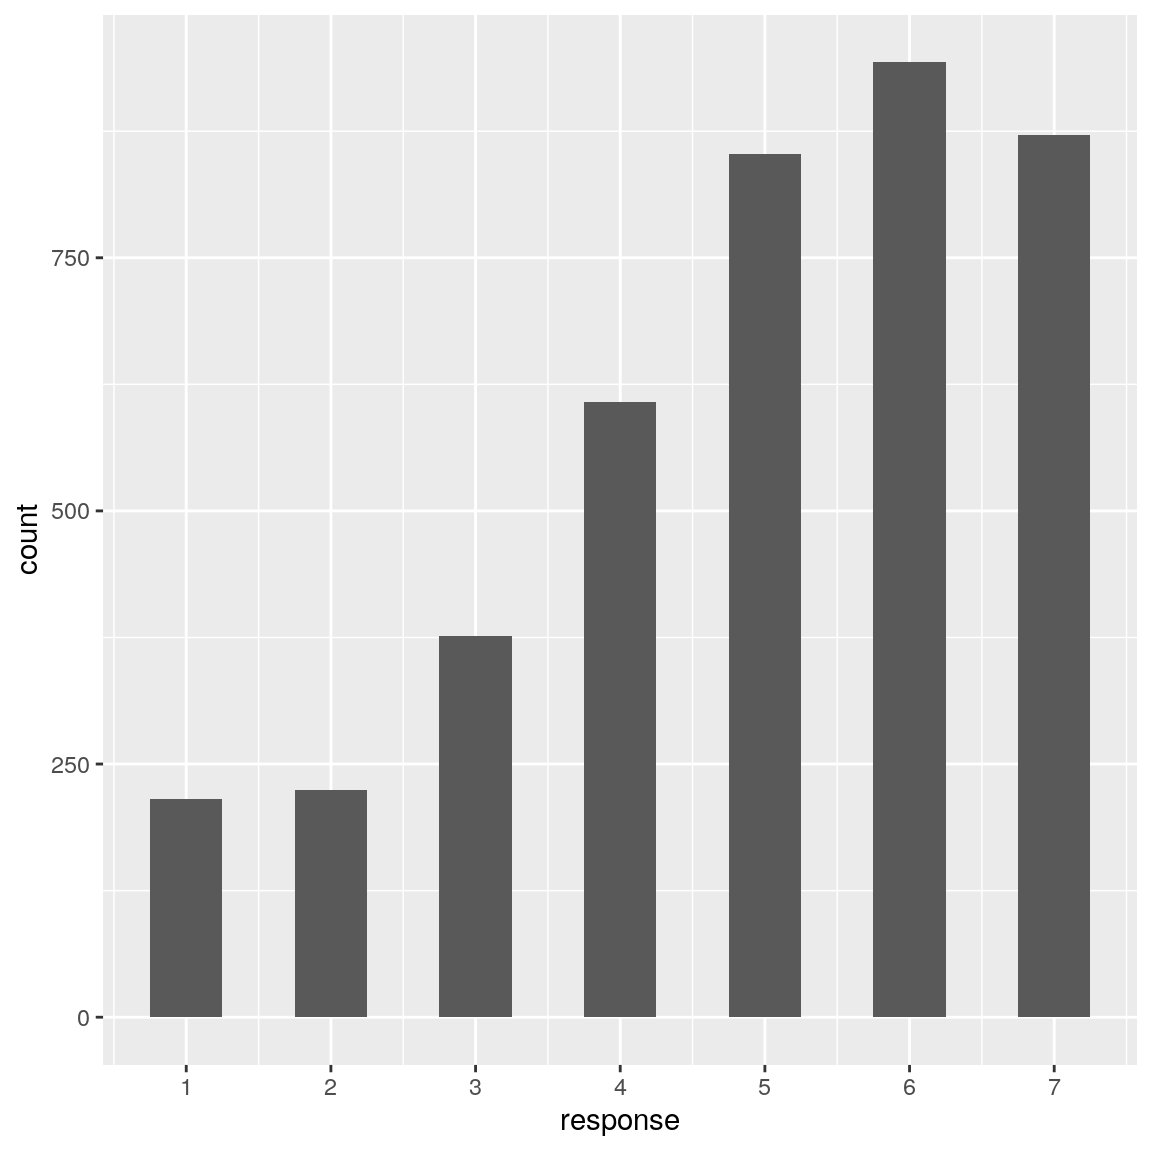
\includegraphics{StatsThinking21_files/figure-latex/unnamed-chunk-43-1.pdf}

It looks like responses were fairly positively overall.

We can also aggregate each participant's responses to each question during each year of their study at Stanford to examine the distribution of mean ATS responses across people by year.

We will use the \texttt{group\_by()} and \texttt{summarize()} functions to aggregate the responses.

\begin{Shaded}
\begin{Highlighting}[]
\NormalTok{attitudeData_agg <-}
\StringTok{  }\NormalTok{attitudeData_long }\OperatorTok\StringTok{ }
\StringTok{  }\KeywordTok{group_by}\NormalTok{(ID, Year) }\OperatorTok
\StringTok{  }\KeywordTok{summarize}\NormalTok{(}
    \DataTypeTok{mean_response =} \KeywordTok{mean}\NormalTok{(response)}
\NormalTok{  )}
\NormalTok{attitudeData_agg}
\end{Highlighting}
\end{Shaded}

\begin{verbatim}
## # A tibble: 141 x 3
## # Groups:   ID [141]
##    ID     Year mean_response
##    <chr> <dbl>         <dbl>
##  1 1         3          6   
##  2 10        2          4.66
##  3 100       4          5.03
##  4 101       2          5.10
##  5 102       3          4.66
##  6 103       2          5.55
##  7 104       2          4.31
##  8 105       3          5.10
##  9 106       1          4.21
## 10 107       2          2.45
## # ... with 131 more rows
\end{verbatim}

First let's use the geom\_density argument in \texttt{ggplot()} to look at mean responses across people, ignoring year of response. The density argrument is like a histogram but smooths things over a bit.

\begin{Shaded}
\begin{Highlighting}[]
\NormalTok{attitudeData_agg }\OperatorTok\StringTok{ }
\StringTok{  }\KeywordTok{ggplot}\NormalTok{(}\KeywordTok{aes}\NormalTok{(mean_response)) }\OperatorTok{+}
\StringTok{  }\KeywordTok{geom_density}\NormalTok{()}
\end{Highlighting}
\end{Shaded}

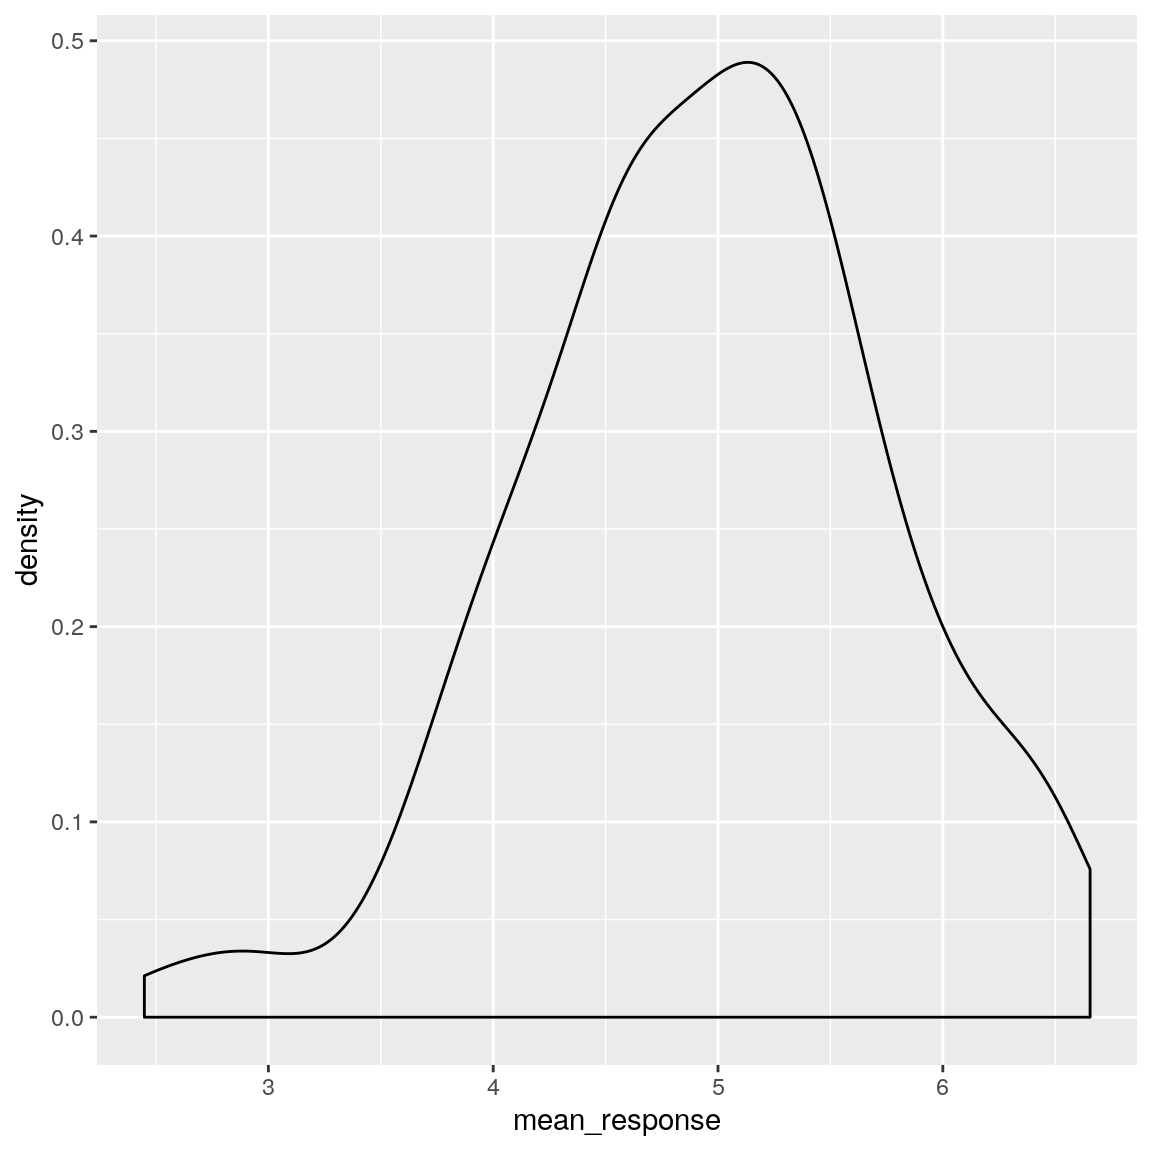
\includegraphics{StatsThinking21_files/figure-latex/unnamed-chunk-45-1.pdf}

Now we can also look at the distribution for each year.

\begin{Shaded}
\begin{Highlighting}[]
\NormalTok{attitudeData_agg }\OperatorTok\StringTok{ }
\StringTok{  }\KeywordTok{ggplot}\NormalTok{(}\KeywordTok{aes}\NormalTok{(mean_response, }\DataTypeTok{color =} \KeywordTok{factor}\NormalTok{(Year))) }\OperatorTok{+}
\StringTok{  }\KeywordTok{geom_density}\NormalTok{()}
\end{Highlighting}
\end{Shaded}

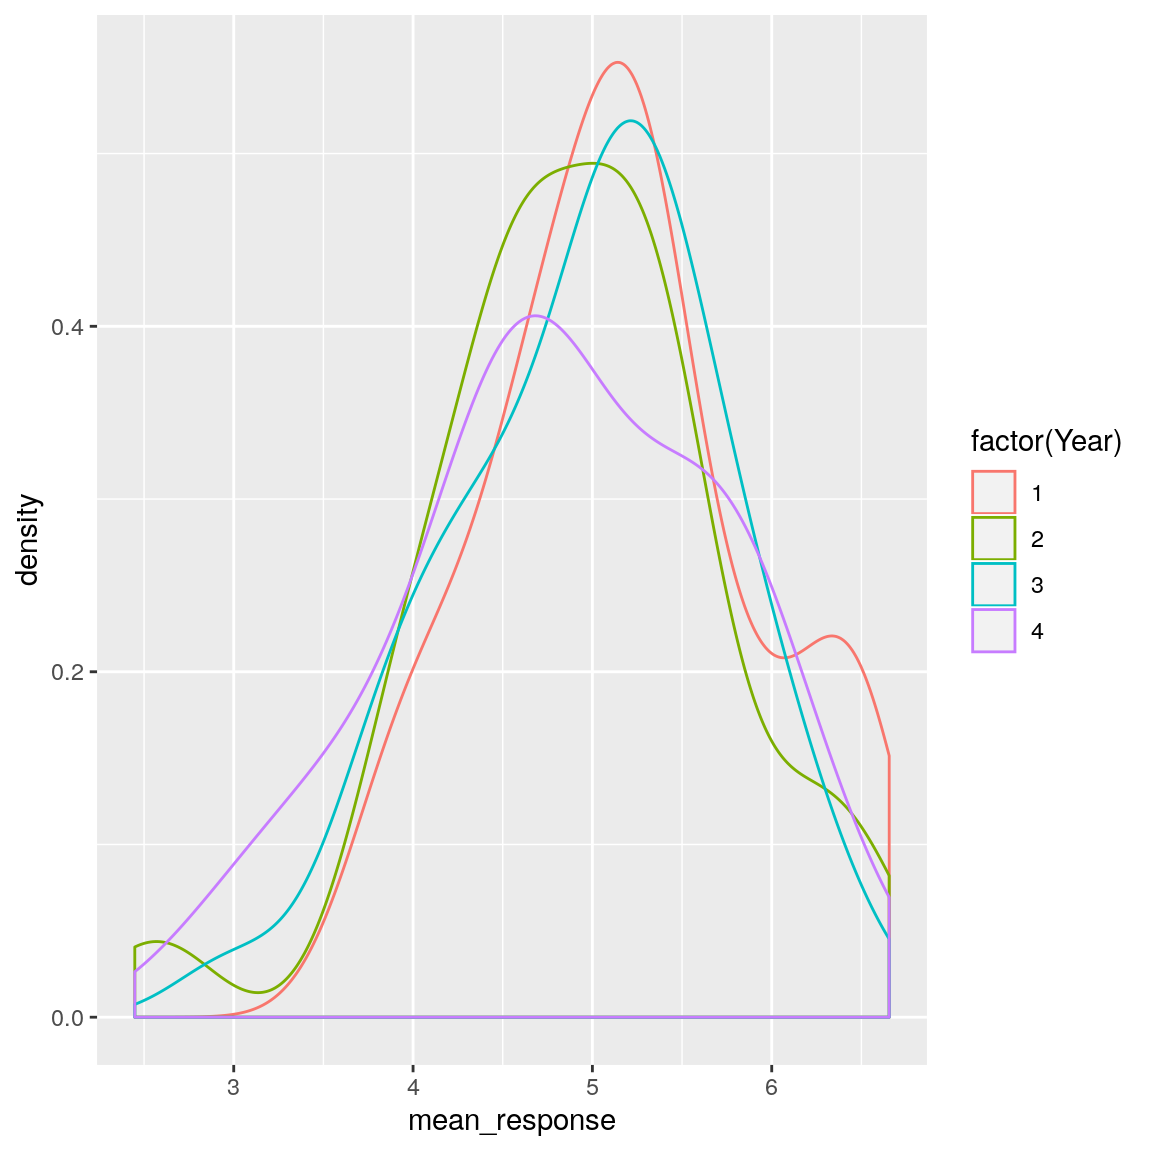
\includegraphics{StatsThinking21_files/figure-latex/unnamed-chunk-46-1.pdf}

Or look at trends in responses across years.

\begin{Shaded}
\begin{Highlighting}[]
\NormalTok{attitudeData_agg }\OperatorTok\StringTok{ }
\StringTok{  }\KeywordTok{group_by}\NormalTok{(Year) }\OperatorTok\StringTok{ }
\StringTok{  }\KeywordTok{summarise}\NormalTok{(}
    \DataTypeTok{mean_response =} \KeywordTok{mean}\NormalTok{(mean_response)}
\NormalTok{  ) }\OperatorTok\StringTok{ }
\StringTok{  }\KeywordTok{ggplot}\NormalTok{(}\KeywordTok{aes}\NormalTok{(Year, mean_response)) }\OperatorTok{+}
\StringTok{  }\KeywordTok{geom_line}\NormalTok{()}
\end{Highlighting}
\end{Shaded}

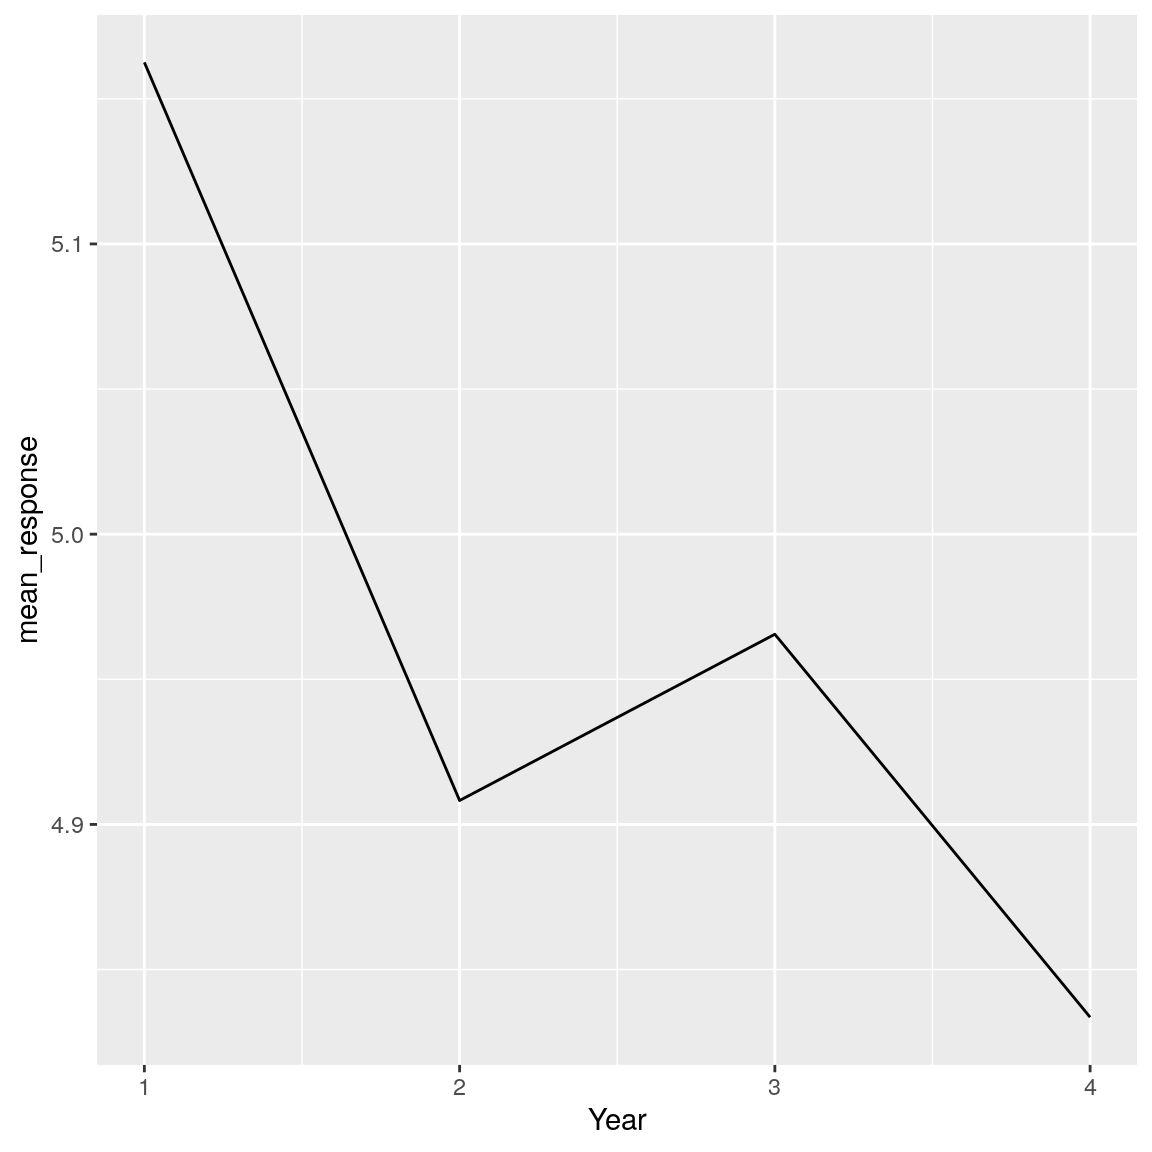
\includegraphics{StatsThinking21_files/figure-latex/unnamed-chunk-47-1.pdf}

This looks like a precipitous drop - but how might that be misleading?

\hypertarget{data-visualization-with-r-with-anna-khazenzon}{%
\chapter{Data visualization with R (with Anna Khazenzon)}\label{data-visualization-with-r-with-anna-khazenzon}}

There are many different tools for plotting data in R, but we will focus on the \texttt{ggplot()} function provided by a package called \texttt{ggplot2}. ggplot is very powerful, but using it requires getting one's head around how it works.

\hypertarget{the-grammar-of-graphics}{%
\section{The grammar of graphics}\label{the-grammar-of-graphics}}

or, the ``gg'' in ggplot

Each language has a grammar consisting of types of words and the rules with which to string them together into sentences. If a sentence is grammatically correct, we're able to parse it, even though that doesn't ensure that it's interesting, beautiful, or even meaningful.

Similarly, plots can be divided up into their core components, which come together via a set of rules.

Some of the major components are :

\begin{itemize}
\tightlist
\item
  data
\item
  aesthetics
\item
  geometries
\item
  themes
\end{itemize}

The data are the actual variables we're plotting, which we pass to ggplot through the data argument. As you've learned, ggplot takes a \textbf{dataframe} in which each column is a variable.

Now we need to tell ggplot \emph{how} to plot those variables, by mapping each variable to an \emph{axis} of the plot. You've seen that when we plot histograms, our variable goes on the x axis. Hence, we set \texttt{x=\textless{}variable\textgreater{}} in a call to \texttt{aes()} within \texttt{ggplot()}. This sets \textbf{aesthetics}, which are mappings of data to certain scales, like axes or things like color or shape. The plot still had two axes -- x and y -- but we didn't need to \emph{specify} what went on the y axis because ggplot knew by \emph{default} that it should make a count variable.

How was ggplot able to figure that out? Because of \textbf{geometries}, which are \emph{shapes} we use to represent our data. You've seen \texttt{geom\_histogram}, which basically gives our graph a bar plot shape, except that it also sets the default y axis variable to be \texttt{count}. Other shapes include points and lines, among many others.

We'll go over other aspects of the grammar of graphics (such as facets, statistics, and coordinates) as they come up. Let's start visualizing some data by first choosing a \textbf{theme}, which describes all of the non-data ink in our plot, like grid lines and text.

\hypertarget{getting-started}{%
\section{Getting started}\label{getting-started}}

Load ggplot and choose a theme you like (see \href{https://bookdown.org/asmundhreinn/r4ds-master/graphics-for-communication.html\#themes}{here} for examples).

\begin{Shaded}
\begin{Highlighting}[]
\KeywordTok{library}\NormalTok{(tidyverse)}

\KeywordTok{theme_set}\NormalTok{(}\KeywordTok{theme_bw}\NormalTok{()) }\CommentTok{# I like this fairly minimal one}
\end{Highlighting}
\end{Shaded}

\hypertarget{lets-think-through-a-visualization}{%
\section{Let's think through a visualization}\label{lets-think-through-a-visualization}}

Principles we want to keep in mind:

\begin{itemize}
\tightlist
\item
  Show the data without distortion
\item
  Use color, shape, and location to encourage comparisons
\item
  Minimize visual clutter (maximize your information to ink ratio)
\end{itemize}

The two questions you want to ask yourself before getting started are:

\begin{itemize}
\tightlist
\item
  What type of variable(s) am I plotting?
\item
  What comparison do I want to make salient for the viewer (possibly myself)?
\end{itemize}

Figuring out \emph{how} to highlight a comparison and include relevant variables usually benefits from sketching the plot out first.

\hypertarget{plotting-the-distribution-of-a-single-variable}{%
\section{Plotting the distribution of a single variable}\label{plotting-the-distribution-of-a-single-variable}}

How do you choose which \textbf{geometry} to use? ggplot allows you to choose from a number of geometries. This choice will determine what sort of plot you create. We will use the built-in mpg dataset, which contains fuel efficiency data for a number of different cars.

\hypertarget{histogram}{%
\subsection{Histogram}\label{histogram}}

The histogram shows the overall distribution of the data. Here we use the nclass.FD function to compute the optimal bin size.

\begin{Shaded}
\begin{Highlighting}[]
\KeywordTok{ggplot}\NormalTok{(mpg, }\KeywordTok{aes}\NormalTok{(hwy)) }\OperatorTok{+}
\StringTok{  }\KeywordTok{geom_histogram}\NormalTok{(}\DataTypeTok{bins =} \KeywordTok{nclass.FD}\NormalTok{(mpg}\OperatorTok{$}\NormalTok{hwy)) }\OperatorTok{+}
\StringTok{  }\KeywordTok{xlab}\NormalTok{(}\StringTok{'Highway mileage'}\NormalTok{) }
\end{Highlighting}
\end{Shaded}

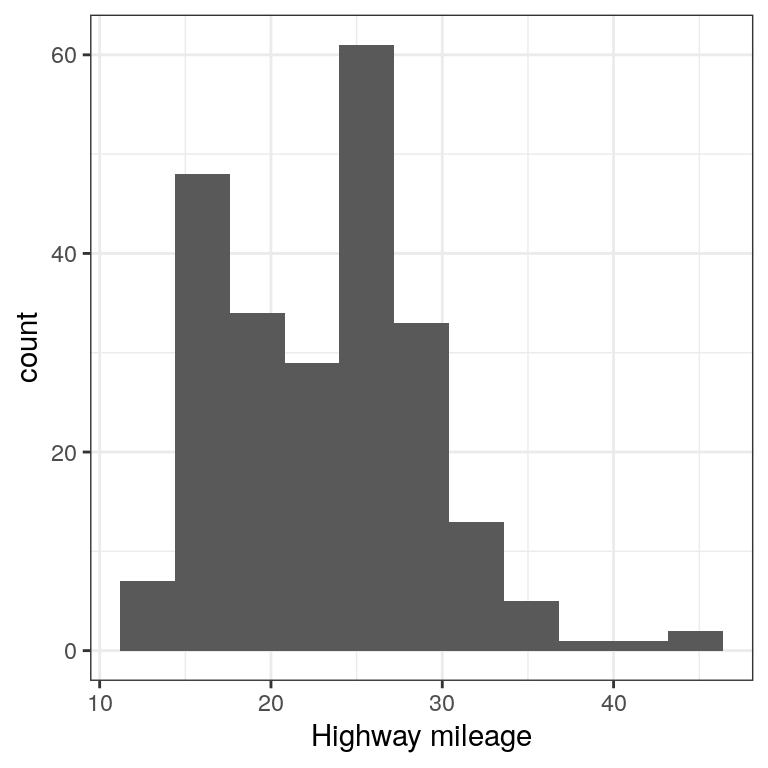
\includegraphics[width=0.5\linewidth]{StatsThinking21_files/figure-latex/unnamed-chunk-50-1}

Instead of creating discrete bins, we can look at relative density continuously.

\hypertarget{density-plot}{%
\subsection{Density plot}\label{density-plot}}

\begin{Shaded}
\begin{Highlighting}[]
\KeywordTok{ggplot}\NormalTok{(mpg, }\KeywordTok{aes}\NormalTok{(hwy)) }\OperatorTok{+}
\StringTok{  }\KeywordTok{geom_density}\NormalTok{() }\OperatorTok{+}
\StringTok{  }\KeywordTok{xlab}\NormalTok{(}\StringTok{'Highway mileage'}\NormalTok{) }
\end{Highlighting}
\end{Shaded}

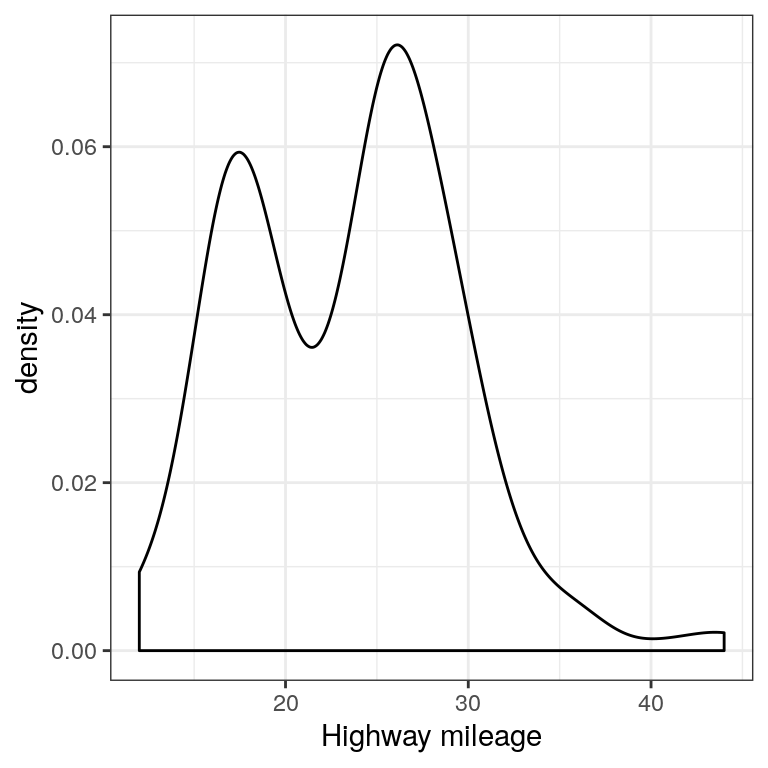
\includegraphics[width=0.5\linewidth]{StatsThinking21_files/figure-latex/unnamed-chunk-51-1}

A note on defaults: The default statistic (or ``stat'') underlying \texttt{geom\_density} is called ``density'' -- not surprising. The default stat for \texttt{geom\_histogram} is ``count''. What do you think would happen if you overrode the default and set \texttt{stat="count"}?

\begin{verbatim}
ggplot(mpg, aes(hwy)) +
  geom_density(stat = "count")
\end{verbatim}

What we discover is that the \emph{geometric} difference between \texttt{geom\_histogram} and \texttt{geom\_density} can actually be generalized. \texttt{geom\_histogram} is a shortcut for working with \texttt{geom\_bar}, and \texttt{geom\_density} is a shortcut for working with \texttt{geom\_line}.

\hypertarget{bar-vs.line-plots}{%
\subsection{Bar vs.~line plots}\label{bar-vs.line-plots}}

\begin{Shaded}
\begin{Highlighting}[]
\KeywordTok{ggplot}\NormalTok{(mpg, }\KeywordTok{aes}\NormalTok{(hwy)) }\OperatorTok{+}
\StringTok{  }\KeywordTok{geom_bar}\NormalTok{(}\DataTypeTok{stat =} \StringTok{"count"}\NormalTok{)}
\end{Highlighting}
\end{Shaded}

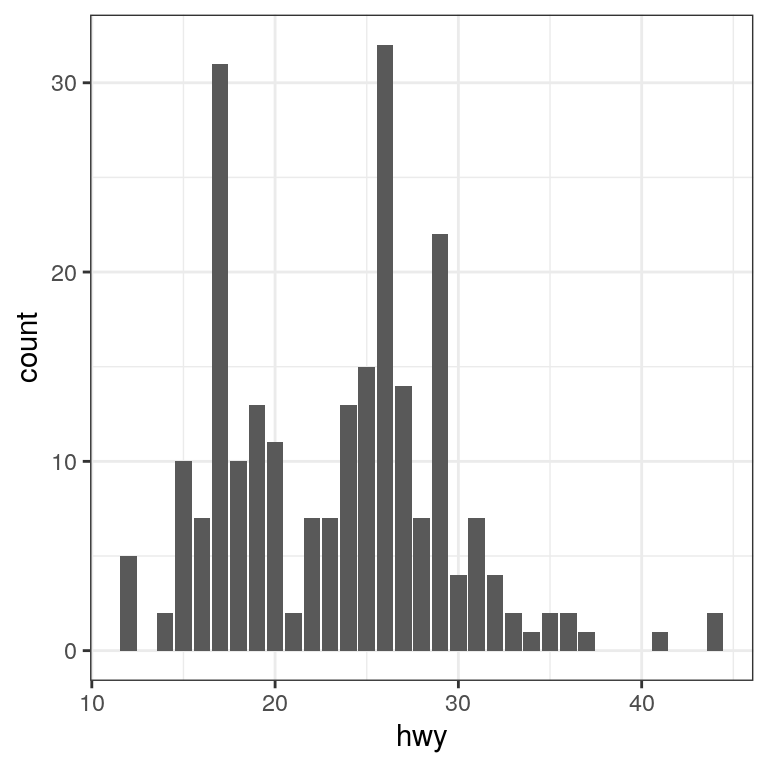
\includegraphics[width=0.5\linewidth]{StatsThinking21_files/figure-latex/unnamed-chunk-52-1}

Note that the geometry tells ggplot what kind of plot to use, and the statistic (\emph{stat}) tells it what kind of summary to present.

\begin{Shaded}
\begin{Highlighting}[]
\KeywordTok{ggplot}\NormalTok{(mpg, }\KeywordTok{aes}\NormalTok{(hwy)) }\OperatorTok{+}
\StringTok{  }\KeywordTok{geom_line}\NormalTok{(}\DataTypeTok{stat =} \StringTok{"density"}\NormalTok{)}
\end{Highlighting}
\end{Shaded}

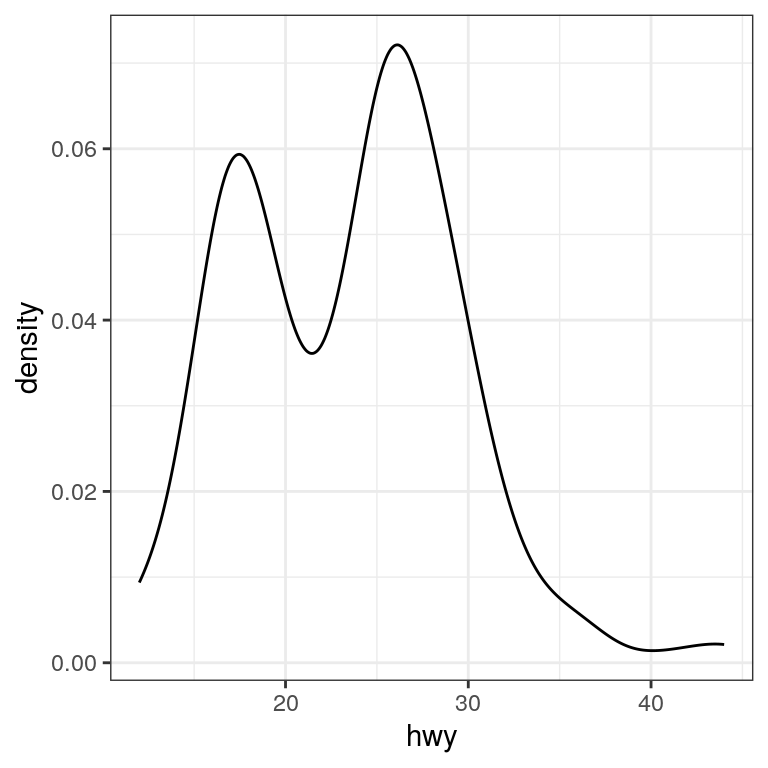
\includegraphics[width=0.5\linewidth]{StatsThinking21_files/figure-latex/unnamed-chunk-53-1}

\hypertarget{plots-with-two-variables}{%
\section{Plots with two variables}\label{plots-with-two-variables}}

Let's check out mileage by car manufacturer. We'll plot one \emph{continuous} variable by one \emph{nominal} one.

First, let's make a bar plot by choosing the stat ``summary'' and picking the ``mean'' function to summarize the data.

\begin{Shaded}
\begin{Highlighting}[]
\KeywordTok{ggplot}\NormalTok{(mpg, }\KeywordTok{aes}\NormalTok{(manufacturer, hwy)) }\OperatorTok{+}
\StringTok{  }\KeywordTok{geom_bar}\NormalTok{(}\DataTypeTok{stat =} \StringTok{"summary"}\NormalTok{, }\DataTypeTok{fun.y =} \StringTok{"mean"}\NormalTok{)  }\OperatorTok{+}\StringTok{ }
\StringTok{  }\KeywordTok{ylab}\NormalTok{(}\StringTok{'Highway mileage'}\NormalTok{)}
\end{Highlighting}
\end{Shaded}

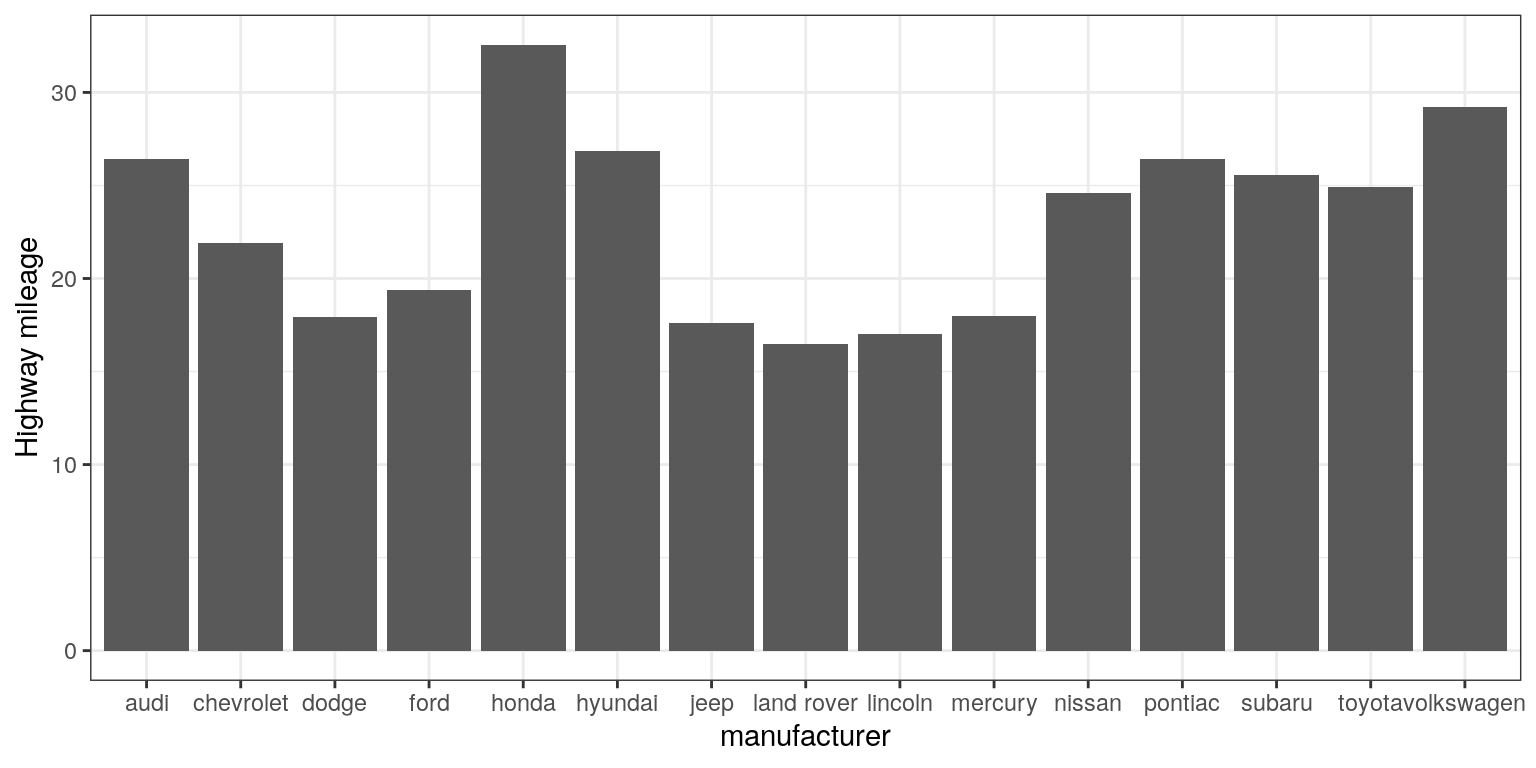
\includegraphics[width=0.8\linewidth]{StatsThinking21_files/figure-latex/unnamed-chunk-54-1}

One problem with this plot is that it's hard to read some of the labels because they overlap. How could we fix that? Hint: search the web for ``ggplot rotate x axis labels'' and add the appropriate command.

\emph{TBD: fix}

\begin{Shaded}
\begin{Highlighting}[]
\KeywordTok{ggplot}\NormalTok{(mpg, }\KeywordTok{aes}\NormalTok{(manufacturer, hwy)) }\OperatorTok{+}
\StringTok{  }\KeywordTok{geom_bar}\NormalTok{(}\DataTypeTok{stat =} \StringTok{"summary"}\NormalTok{, }\DataTypeTok{fun.y =} \StringTok{"mean"}\NormalTok{)  }\OperatorTok{+}\StringTok{ }
\StringTok{  }\KeywordTok{ylab}\NormalTok{(}\StringTok{'Highway mileage'}\NormalTok{)}
\end{Highlighting}
\end{Shaded}

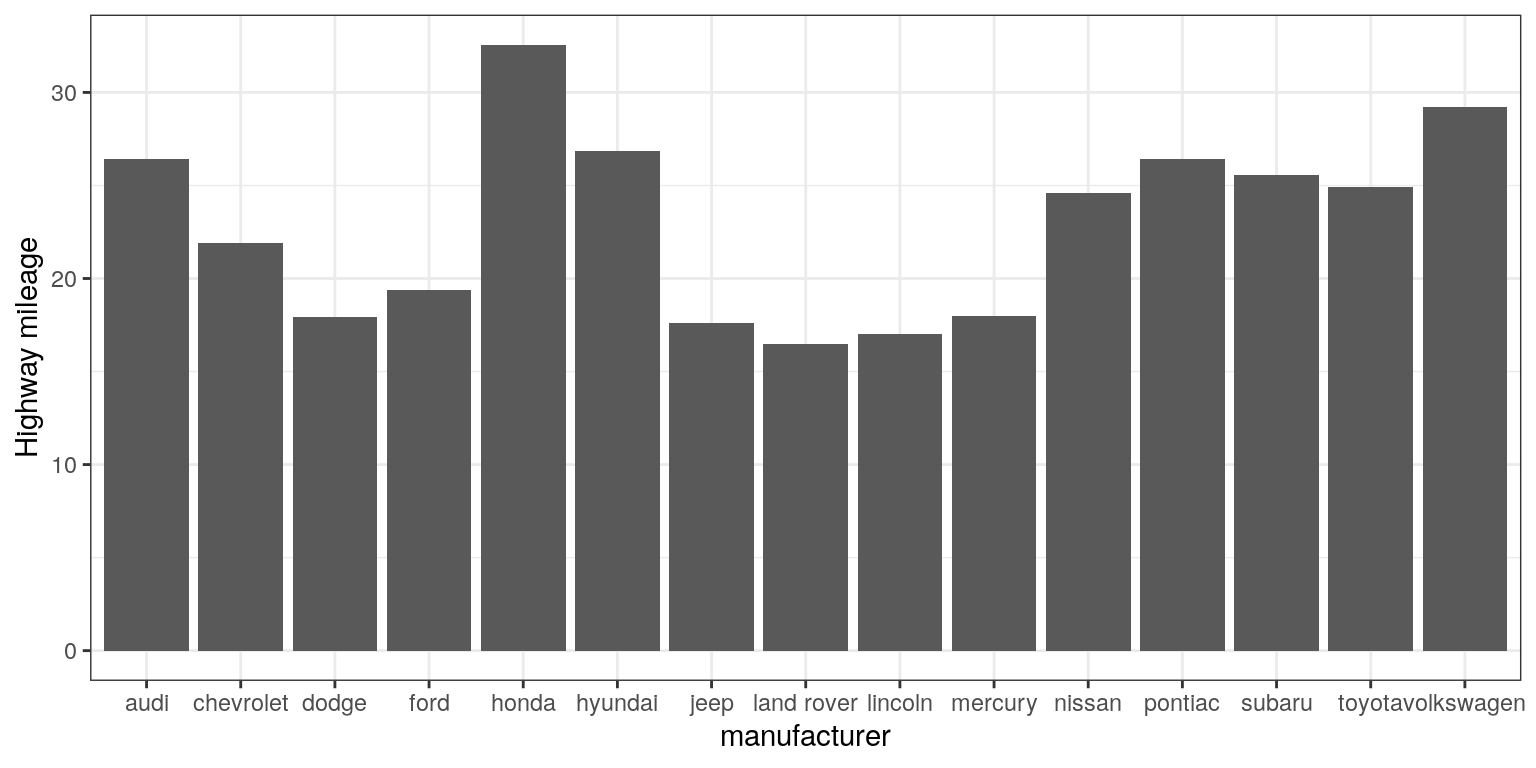
\includegraphics[width=0.8\linewidth]{StatsThinking21_files/figure-latex/unnamed-chunk-55-1}

\hypertarget{adding-on-variables}{%
\subsection{Adding on variables}\label{adding-on-variables}}

What if we wanted to add another variable into the mix? Maybe the \emph{year} of the car is also important to consider. We have a few options here. First, you could map the variable to another \textbf{aesthetic}.

\begin{Shaded}
\begin{Highlighting}[]
\CommentTok{# first, year needs to be converted to a factor}
\NormalTok{mpg}\OperatorTok{$}\NormalTok{year <-}\StringTok{ }\KeywordTok{factor}\NormalTok{(mpg}\OperatorTok{$}\NormalTok{year) }

\KeywordTok{ggplot}\NormalTok{(mpg, }\KeywordTok{aes}\NormalTok{(manufacturer, hwy, }\DataTypeTok{fill =}\NormalTok{ year)) }\OperatorTok{+}
\StringTok{  }\KeywordTok{geom_bar}\NormalTok{(}\DataTypeTok{stat =} \StringTok{"summary"}\NormalTok{, }\DataTypeTok{fun.y =} \StringTok{"mean"}\NormalTok{)}
\end{Highlighting}
\end{Shaded}

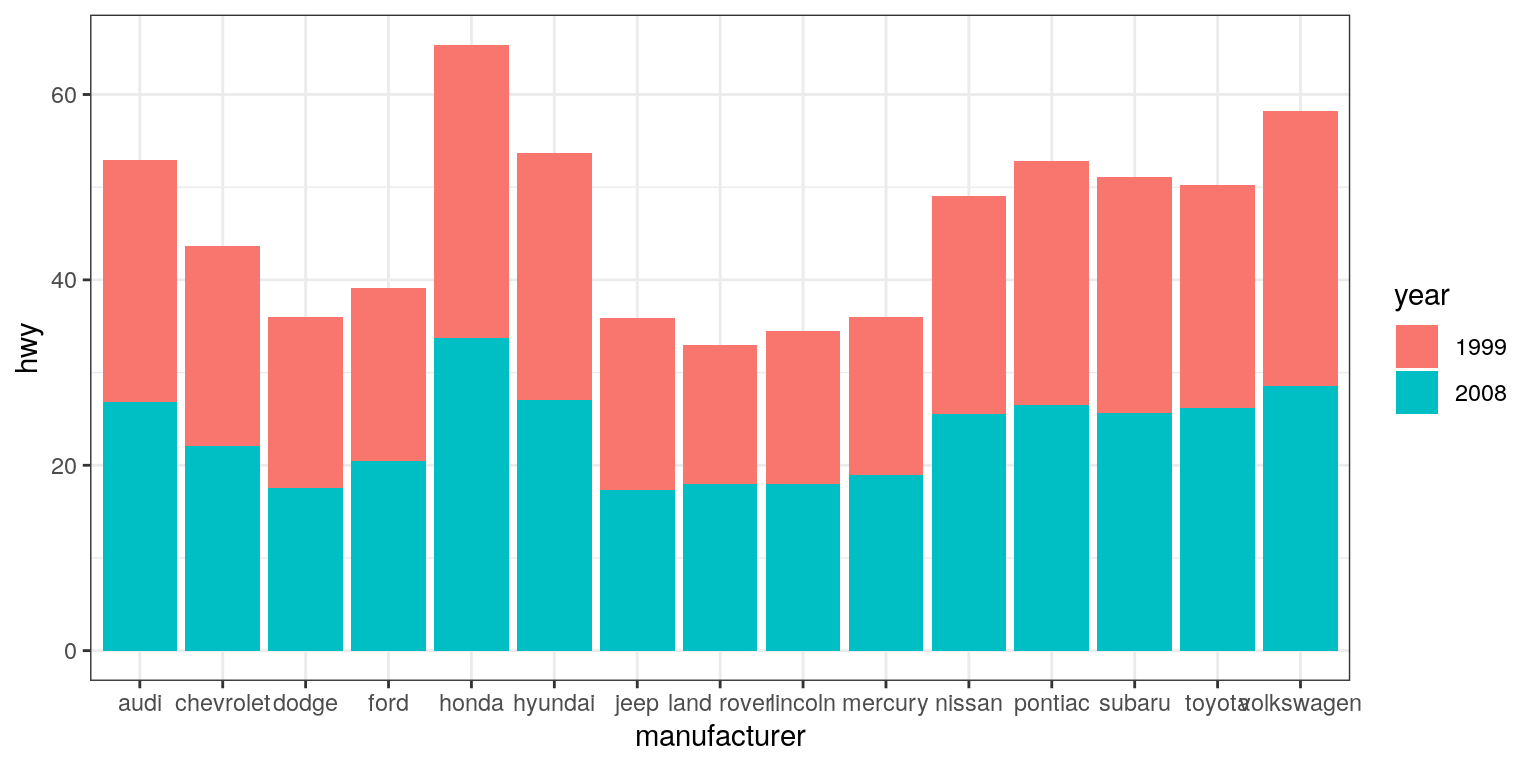
\includegraphics[width=0.8\linewidth]{StatsThinking21_files/figure-latex/unnamed-chunk-56-1}

By default, the bars are \emph{stacked} on top of one another. If you want to separate them, you can change the \texttt{position} argument form its default to ``dodge''.

\begin{Shaded}
\begin{Highlighting}[]
\KeywordTok{ggplot}\NormalTok{(mpg, }\KeywordTok{aes}\NormalTok{(manufacturer, hwy, }\DataTypeTok{fill=}\NormalTok{year)) }\OperatorTok{+}
\StringTok{  }\KeywordTok{geom_bar}\NormalTok{(}\DataTypeTok{stat =} \StringTok{"summary"}\NormalTok{, }
           \DataTypeTok{fun.y =} \StringTok{"mean"}\NormalTok{, }
           \DataTypeTok{position =} \StringTok{"dodge"}\NormalTok{)}
\end{Highlighting}
\end{Shaded}

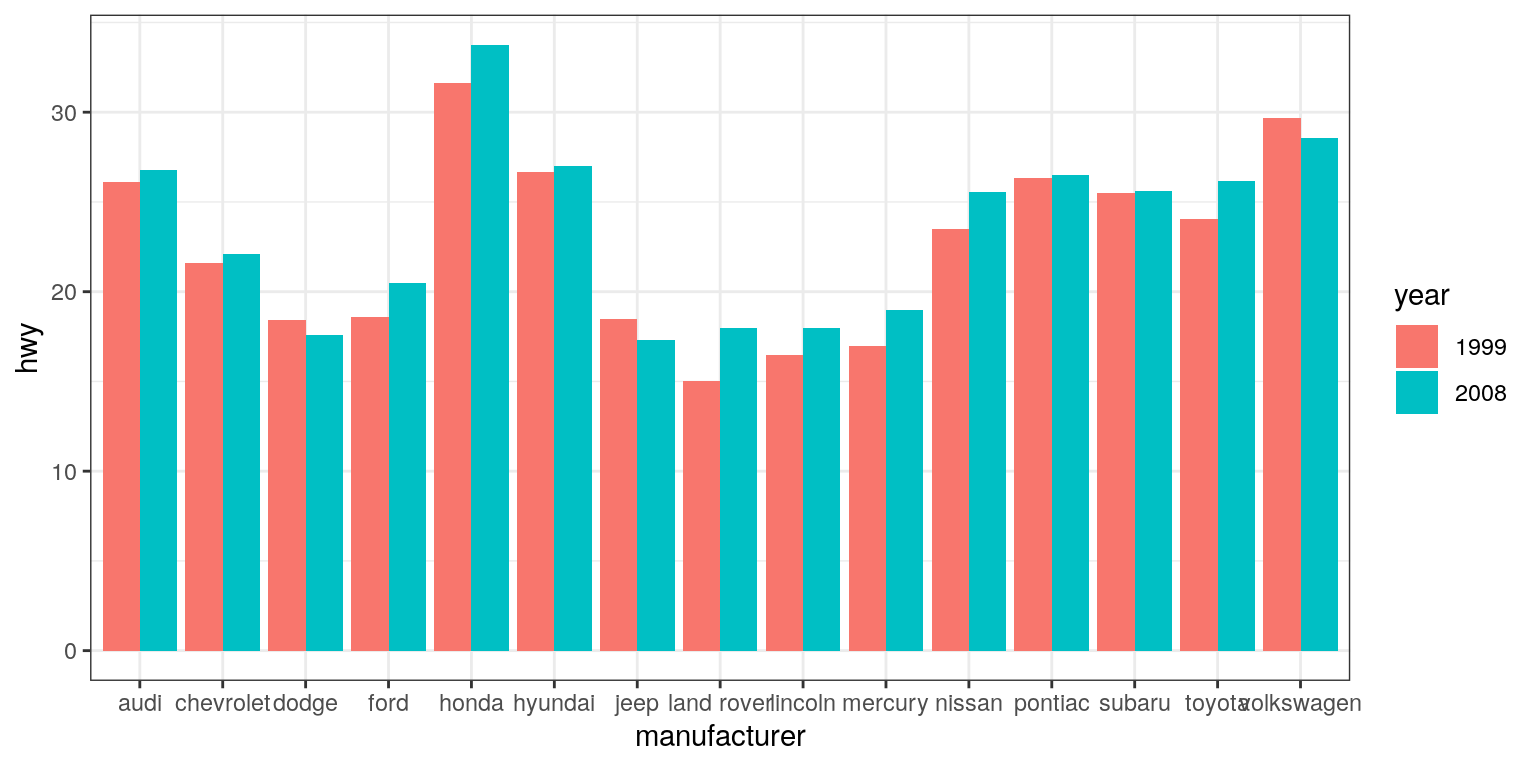
\includegraphics[width=0.8\linewidth]{StatsThinking21_files/figure-latex/unnamed-chunk-57-1}

\begin{Shaded}
\begin{Highlighting}[]
\KeywordTok{ggplot}\NormalTok{(mpg, }\KeywordTok{aes}\NormalTok{(year, hwy, }
                \DataTypeTok{group=}\NormalTok{manufacturer,}
                \DataTypeTok{color=}\NormalTok{manufacturer)) }\OperatorTok{+}
\StringTok{  }\KeywordTok{geom_line}\NormalTok{(}\DataTypeTok{stat =} \StringTok{"summary"}\NormalTok{, }\DataTypeTok{fun.y =} \StringTok{"mean"}\NormalTok{)}
\end{Highlighting}
\end{Shaded}

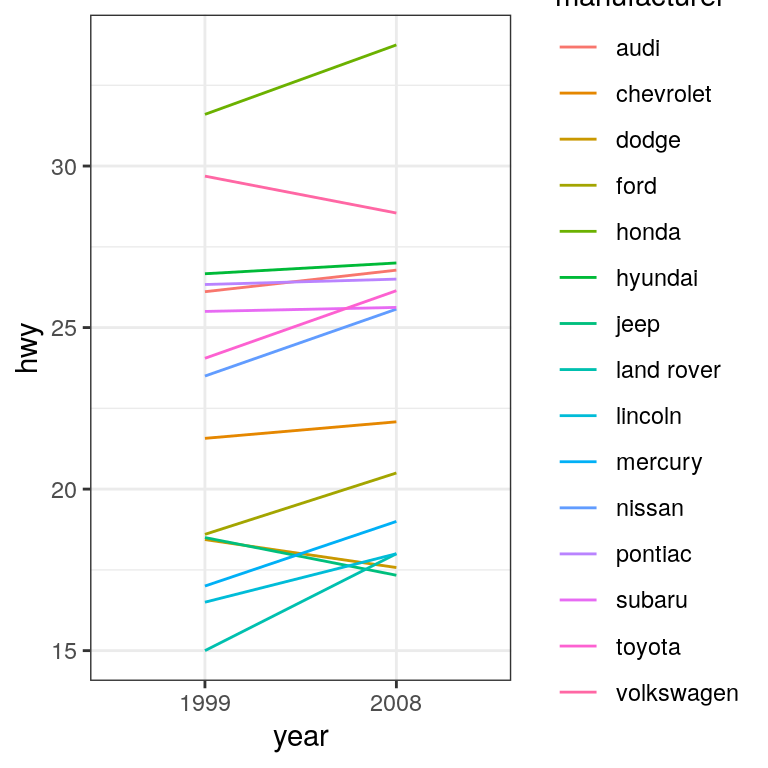
\includegraphics[width=0.5\linewidth]{StatsThinking21_files/figure-latex/unnamed-chunk-58-1}

For a less visually cluttered plot, let's try \textbf{facetting}. This creates \emph{subplots} for each value of the \texttt{year} variable.

\begin{Shaded}
\begin{Highlighting}[]
\KeywordTok{ggplot}\NormalTok{(mpg, }\KeywordTok{aes}\NormalTok{(manufacturer, hwy)) }\OperatorTok{+}
\StringTok{  }\CommentTok{# split up the bar plot into two by year}
\StringTok{  }\KeywordTok{facet_grid}\NormalTok{(year }\OperatorTok{~}\StringTok{ }\NormalTok{.) }\OperatorTok{+}\StringTok{ }
\StringTok{  }\KeywordTok{geom_bar}\NormalTok{(}\DataTypeTok{stat =} \StringTok{"summary"}\NormalTok{, }
           \DataTypeTok{fun.y =} \StringTok{"mean"}\NormalTok{)}
\end{Highlighting}
\end{Shaded}

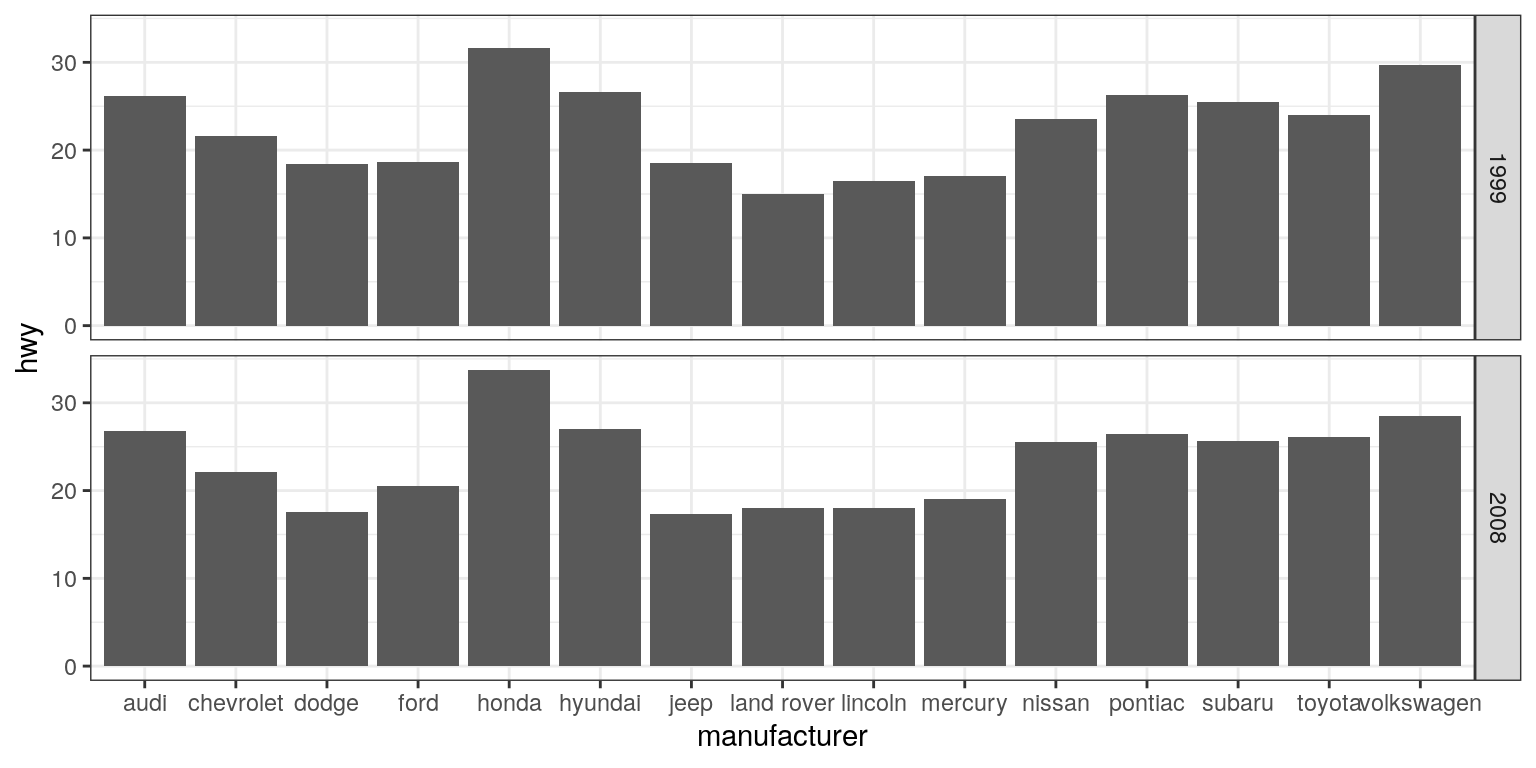
\includegraphics[width=0.8\linewidth]{StatsThinking21_files/figure-latex/unnamed-chunk-59-1}

\hypertarget{plotting-dispersion}{%
\subsection{Plotting dispersion}\label{plotting-dispersion}}

Instead of looking at just the means, we can get a sense of the entire distribution of mileage values for each manufacturer.

\hypertarget{box-plot}{%
\subsubsection{Box plot}\label{box-plot}}

\begin{Shaded}
\begin{Highlighting}[]
\KeywordTok{ggplot}\NormalTok{(mpg, }\KeywordTok{aes}\NormalTok{(manufacturer, hwy)) }\OperatorTok{+}
\StringTok{  }\KeywordTok{geom_boxplot}\NormalTok{()}
\end{Highlighting}
\end{Shaded}

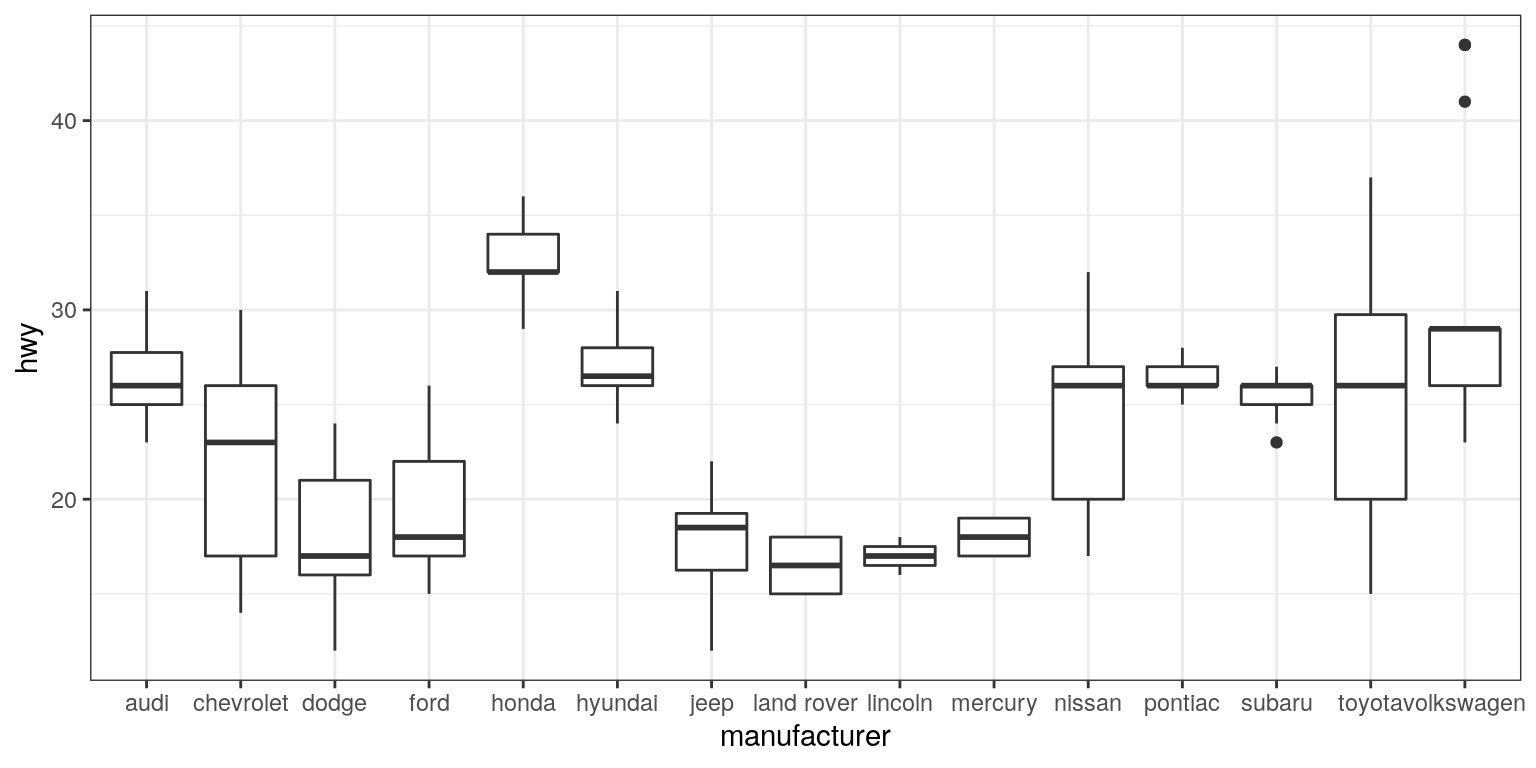
\includegraphics[width=0.8\linewidth]{StatsThinking21_files/figure-latex/unnamed-chunk-60-1}

A \textbf{box plot} (or box and whiskers plot) uses quartiles to give us a sense of spread. The thickest line, somewhere inside the box, represents the \emph{median}. The upper and lower bounds of the box (the \emph{hinges}) are the first and third quartiles (can you use them to approximate the interquartile range?). The lines extending from the hinges are the remaining data points, excluding \textbf{outliers}, which are plotted as individual points.

\hypertarget{error-bars}{%
\subsubsection{Error bars}\label{error-bars}}

Now, let's do something a bit more complex, but much more useful -- let's create our own summary of the data, so we can choose which summary statistic to plot and also compute a measure of dispersion of our choosing.

\begin{Shaded}
\begin{Highlighting}[]
\CommentTok{# summarise data}
\NormalTok{mpg_summary <-}\StringTok{ }\NormalTok{mpg }\OperatorTok
\StringTok{  }\KeywordTok{group_by}\NormalTok{(manufacturer) }\OperatorTok\StringTok{ }
\StringTok{  }\KeywordTok{summarise}\NormalTok{(}\DataTypeTok{n =} \KeywordTok{n}\NormalTok{(), }
            \DataTypeTok{mean_hwy =} \KeywordTok{mean}\NormalTok{(hwy), }
            \DataTypeTok{sd_hwy =} \KeywordTok{sd}\NormalTok{(hwy))}

\CommentTok{# compute confidence intervals for the error bars}
\CommentTok{# (we'll talk about this later in the course!)}

\NormalTok{limits <-}\StringTok{ }\KeywordTok{aes}\NormalTok{(}
  \CommentTok{# compute the lower limit of the error bar}
  \DataTypeTok{ymin =}\NormalTok{ mean_hwy }\OperatorTok{-}\StringTok{ }\FloatTok{1.96} \OperatorTok{*}\StringTok{ }\NormalTok{sd_hwy }\OperatorTok{/}\StringTok{ }\KeywordTok{sqrt}\NormalTok{(n), }
  \CommentTok{# compute the upper limit}
  \DataTypeTok{ymax =}\NormalTok{ mean_hwy }\OperatorTok{+}\StringTok{ }\FloatTok{1.96} \OperatorTok{*}\StringTok{ }\NormalTok{sd_hwy }\OperatorTok{/}\StringTok{ }\KeywordTok{sqrt}\NormalTok{(n))}

\CommentTok{# now we're giving ggplot the mean for each group, }
\CommentTok{# instead of the datapoints themselves}

\KeywordTok{ggplot}\NormalTok{(mpg_summary, }\KeywordTok{aes}\NormalTok{(manufacturer, mean_hwy)) }\OperatorTok{+}
\StringTok{  }\CommentTok{# we set stat = "identity" on the summary data }
\StringTok{  }\KeywordTok{geom_bar}\NormalTok{(}\DataTypeTok{stat =} \StringTok{"identity"}\NormalTok{) }\OperatorTok{+}\StringTok{ }
\StringTok{  }\CommentTok{# we create error bars using the limits we computed above}
\StringTok{  }\KeywordTok{geom_errorbar}\NormalTok{(limits, }\DataTypeTok{width=}\FloatTok{0.5}\NormalTok{) }
\end{Highlighting}
\end{Shaded}

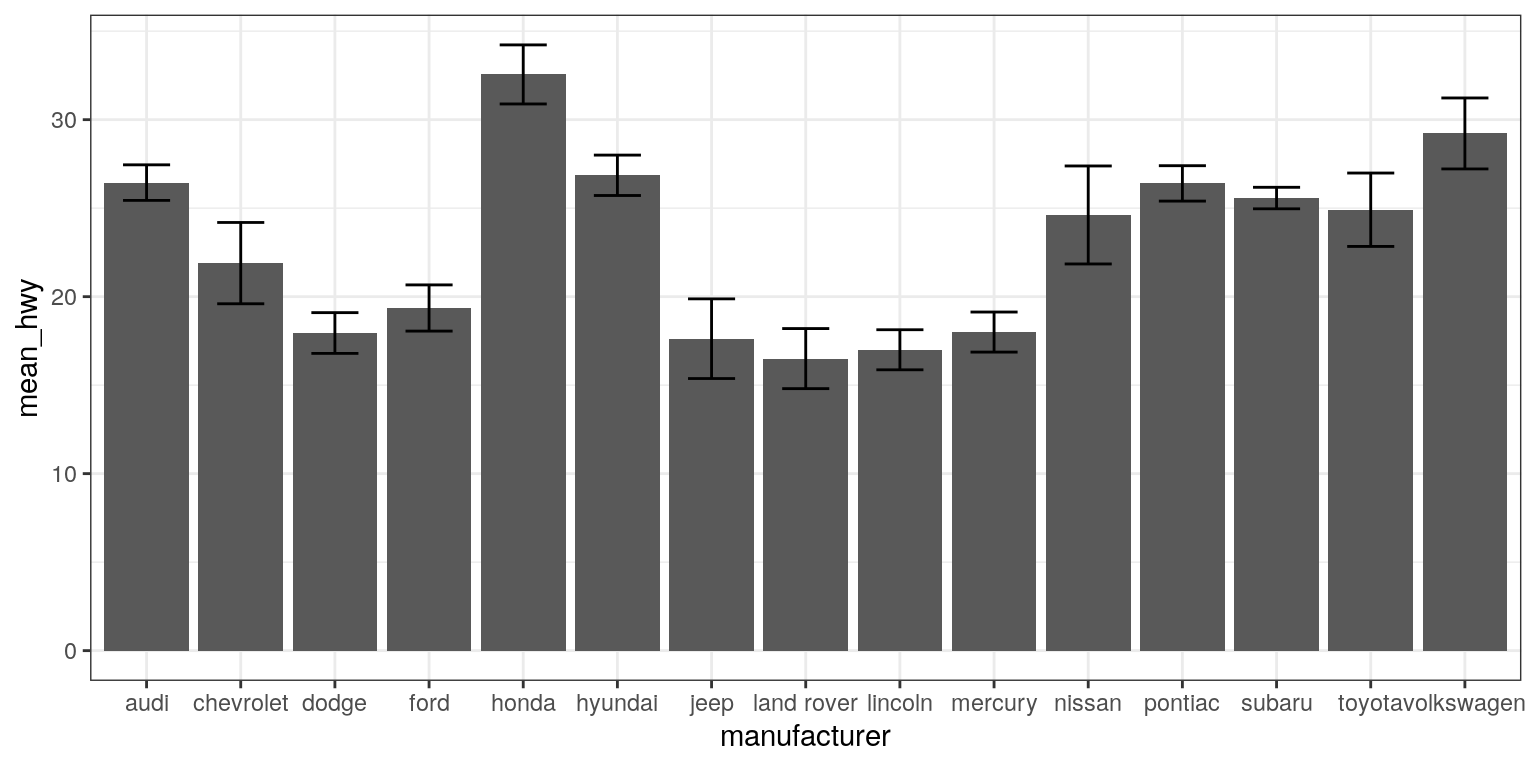
\includegraphics[width=0.8\linewidth]{StatsThinking21_files/figure-latex/unnamed-chunk-61-1}

Error bars don't always mean the same thing -- it's important to determine whether you're looking at e.g.~standard error or confidence intervals (which we'll talk more about later in the course).

\hypertarget{minimizing-non-data-ink}{%
\paragraph{Minimizing non-data ink}\label{minimizing-non-data-ink}}

The plot we just created is nice and all, but it's tough to look at. The bar plots add a lot of ink that doesn't help us compare engine sizes across manufacturers. Similarly, the width of the error bars doesn't add any information. Let's tweak which \emph{geometry} we use, and tweak the appearance of the error bars.

\begin{Shaded}
\begin{Highlighting}[]
\KeywordTok{ggplot}\NormalTok{(mpg_summary, }\KeywordTok{aes}\NormalTok{(manufacturer, mean_hwy)) }\OperatorTok{+}
\StringTok{  }\CommentTok{# switch to point instead of bar to minimize ink used}
\StringTok{  }\KeywordTok{geom_point}\NormalTok{() }\OperatorTok{+}\StringTok{ }
\StringTok{  }\CommentTok{# remove the horizontal parts of the error bars}
\StringTok{  }\KeywordTok{geom_errorbar}\NormalTok{(limits, }\DataTypeTok{width =} \DecValTok{0}\NormalTok{) }
\end{Highlighting}
\end{Shaded}

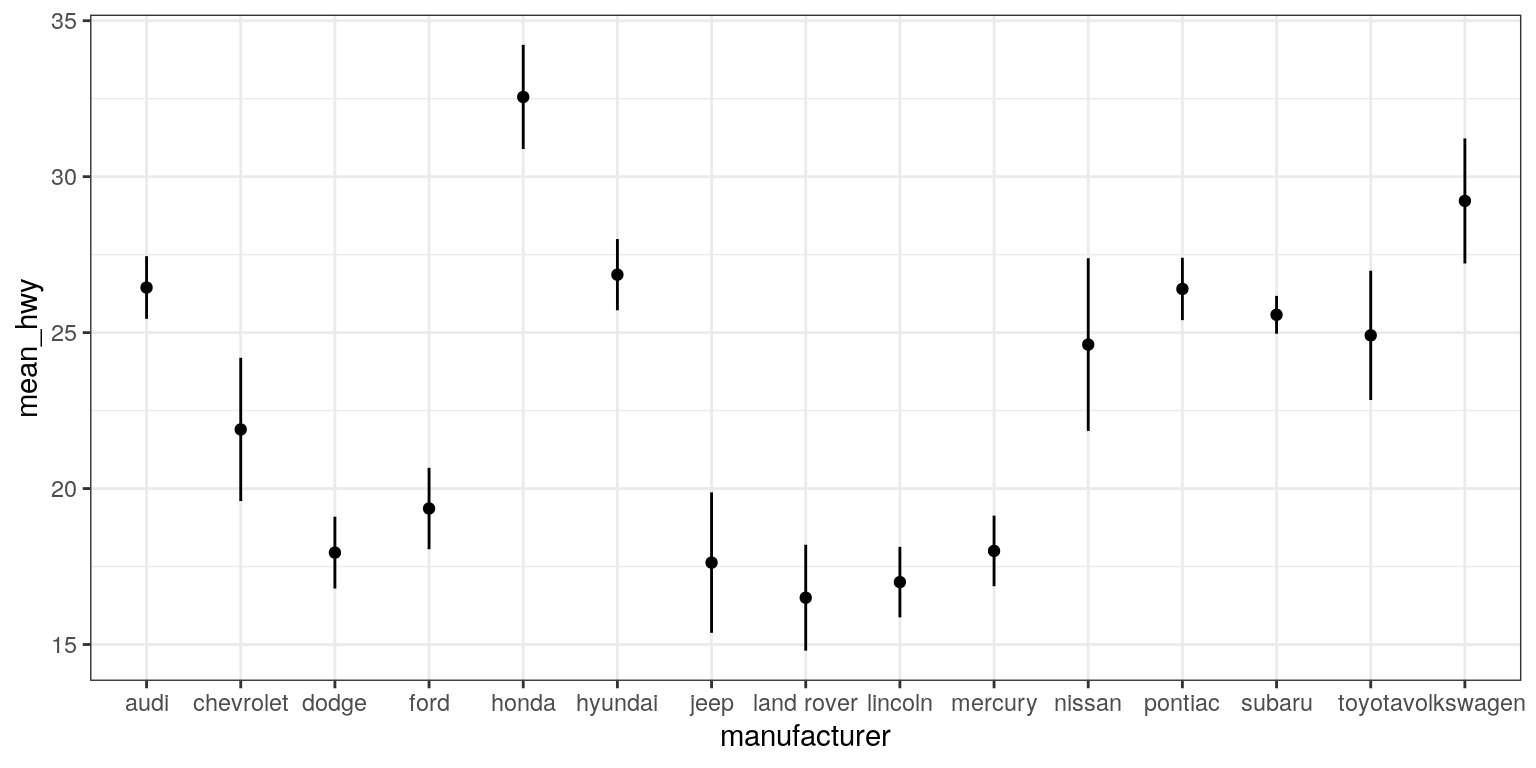
\includegraphics[width=0.8\linewidth]{StatsThinking21_files/figure-latex/unnamed-chunk-62-1}

Looks a lot cleaner, but our points are all over the place. Let's make a final tweak to make \emph{learning something} from this plot a bit easier.

\begin{Shaded}
\begin{Highlighting}[]
\NormalTok{mpg_summary_ordered <-}\StringTok{ }\NormalTok{mpg_summary }\OperatorTok
\StringTok{  }\KeywordTok{mutate}\NormalTok{(}
    \CommentTok{# we sort manufacturers by mean engine size}
    \DataTypeTok{manufacturer =} \KeywordTok{reorder}\NormalTok{(manufacturer, }\OperatorTok{-}\NormalTok{mean_hwy)}
\NormalTok{  )}

\KeywordTok{ggplot}\NormalTok{(mpg_summary_ordered, }\KeywordTok{aes}\NormalTok{(manufacturer, mean_hwy)) }\OperatorTok{+}
\StringTok{  }\KeywordTok{geom_point}\NormalTok{() }\OperatorTok{+}\StringTok{ }
\StringTok{  }\KeywordTok{geom_errorbar}\NormalTok{(limits, }\DataTypeTok{width =} \DecValTok{0}\NormalTok{) }
\end{Highlighting}
\end{Shaded}

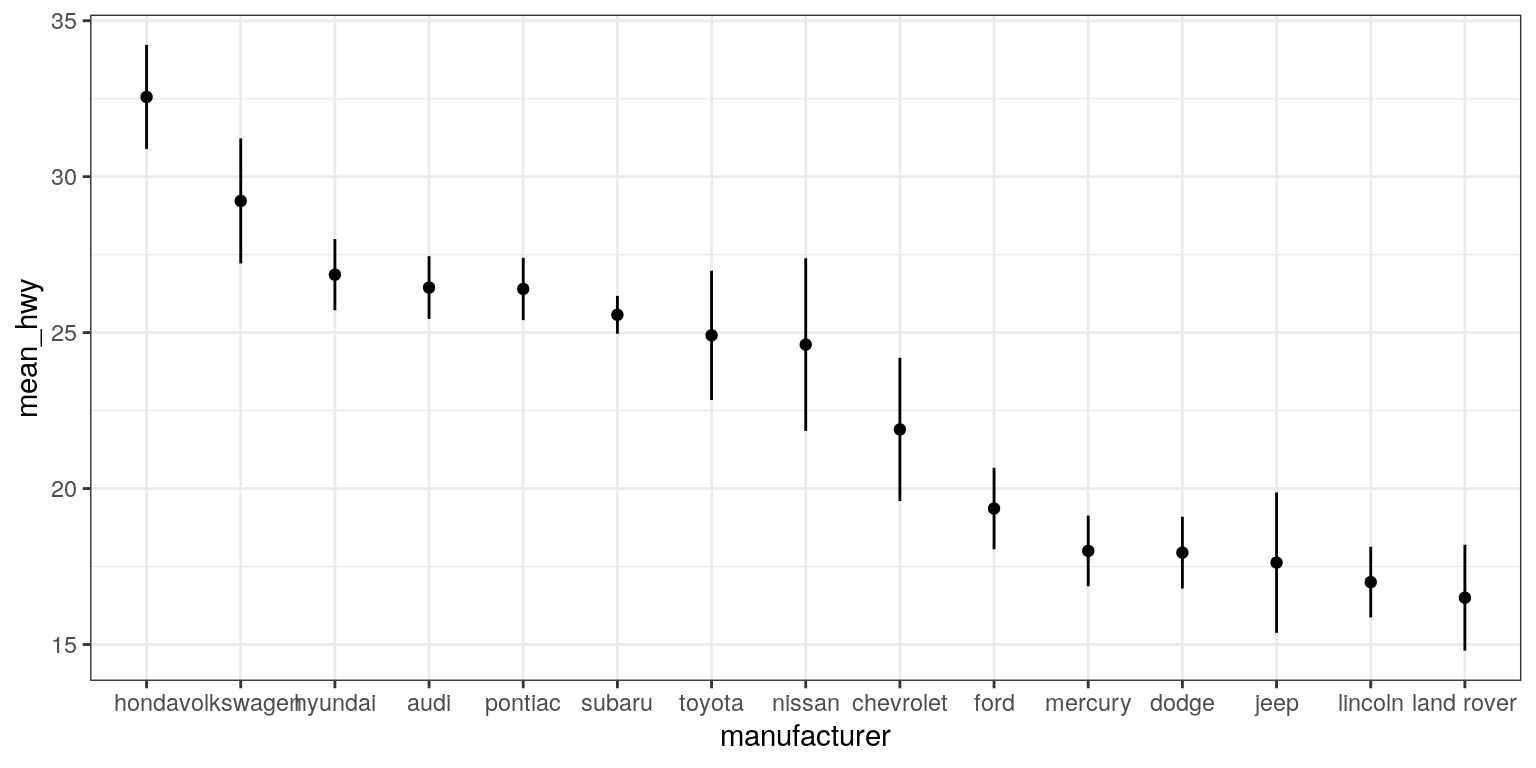
\includegraphics[width=0.8\linewidth]{StatsThinking21_files/figure-latex/unnamed-chunk-63-1}

\hypertarget{scatter-plot}{%
\subsection{Scatter plot}\label{scatter-plot}}

When we have multiple \emph{continuous} variables, we can use points to plot each variable on an axis. This is known as a \textbf{scatter plot}. You've seen this example in your reading.

\begin{Shaded}
\begin{Highlighting}[]
\KeywordTok{ggplot}\NormalTok{(mpg, }\KeywordTok{aes}\NormalTok{(displ, hwy)) }\OperatorTok{+}
\StringTok{  }\KeywordTok{geom_point}\NormalTok{()}
\end{Highlighting}
\end{Shaded}

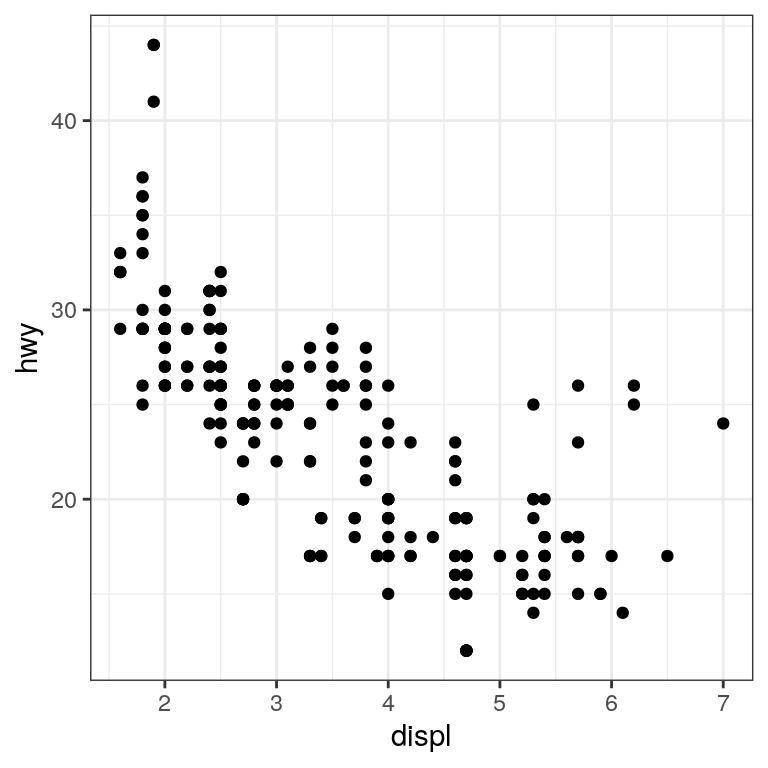
\includegraphics[width=0.5\linewidth]{StatsThinking21_files/figure-latex/unnamed-chunk-64-1}

\hypertarget{layers-of-data}{%
\subsubsection{Layers of data}\label{layers-of-data}}

We can add layers of data onto this graph, like a \emph{line of best fit}. We use a geometry known as a \textbf{smooth} to accomplish this.

\begin{Shaded}
\begin{Highlighting}[]
\KeywordTok{ggplot}\NormalTok{(mpg, }\KeywordTok{aes}\NormalTok{(displ, hwy)) }\OperatorTok{+}
\StringTok{  }\KeywordTok{geom_point}\NormalTok{() }\OperatorTok{+}
\StringTok{  }\KeywordTok{geom_smooth}\NormalTok{(}\DataTypeTok{color =} \StringTok{"black"}\NormalTok{)}
\end{Highlighting}
\end{Shaded}

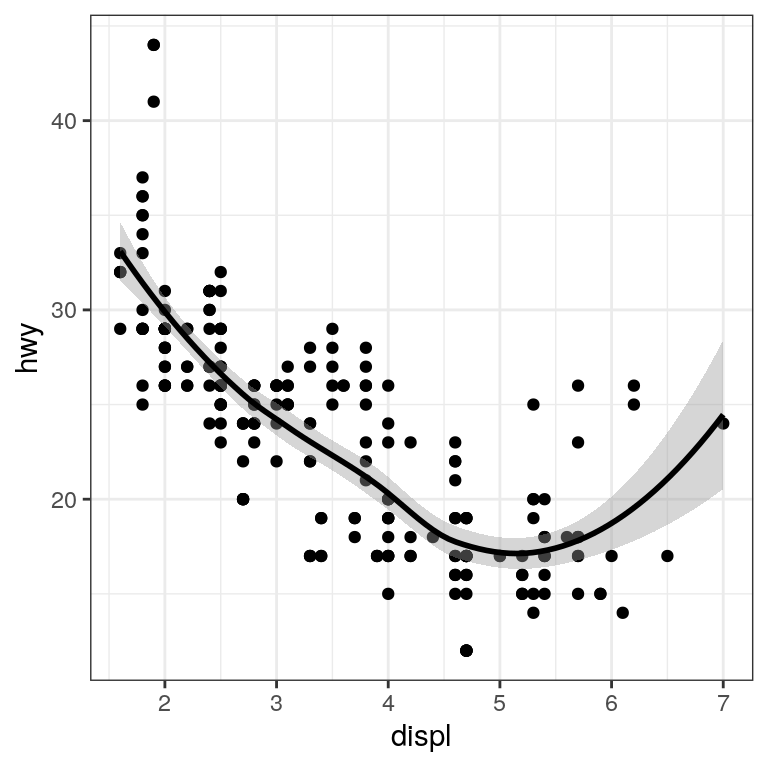
\includegraphics[width=0.5\linewidth]{StatsThinking21_files/figure-latex/unnamed-chunk-65-1}

We can add on points and a smooth line for another set of data as well (efficiency in the city instead of on the highway).

\begin{Shaded}
\begin{Highlighting}[]
\KeywordTok{ggplot}\NormalTok{(mpg) }\OperatorTok{+}
\StringTok{  }\KeywordTok{geom_point}\NormalTok{(}\KeywordTok{aes}\NormalTok{(displ, hwy), }\DataTypeTok{color =} \StringTok{"grey"}\NormalTok{) }\OperatorTok{+}
\StringTok{  }\KeywordTok{geom_smooth}\NormalTok{(}\KeywordTok{aes}\NormalTok{(displ, hwy), }\DataTypeTok{color =} \StringTok{"grey"}\NormalTok{) }\OperatorTok{+}
\StringTok{  }\KeywordTok{geom_point}\NormalTok{(}\KeywordTok{aes}\NormalTok{(displ, cty), }\DataTypeTok{color =} \StringTok{"limegreen"}\NormalTok{) }\OperatorTok{+}
\StringTok{  }\KeywordTok{geom_smooth}\NormalTok{(}\KeywordTok{aes}\NormalTok{(displ, cty), }\DataTypeTok{color =} \StringTok{"limegreen"}\NormalTok{)}
\end{Highlighting}
\end{Shaded}

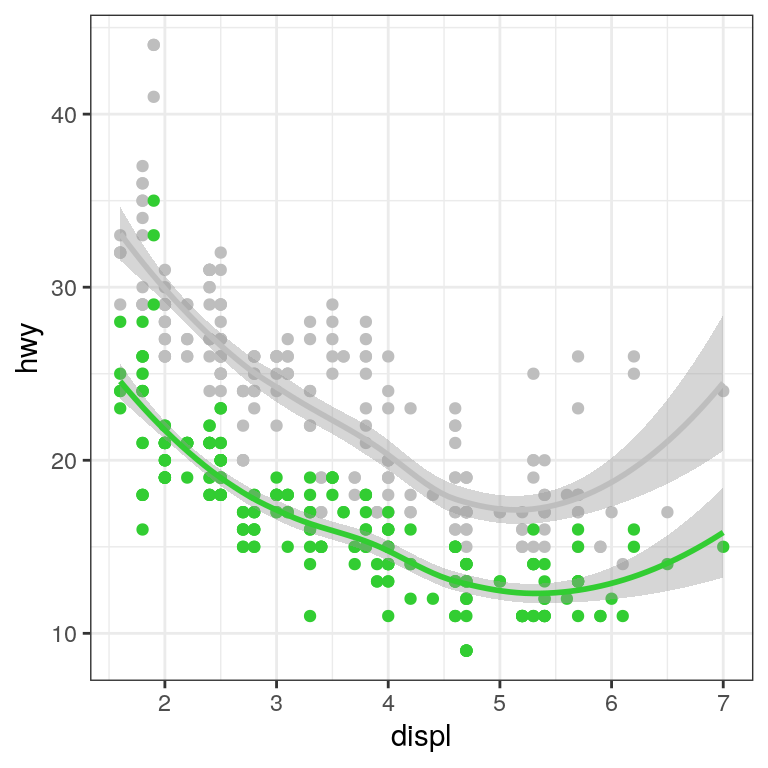
\includegraphics[width=0.5\linewidth]{StatsThinking21_files/figure-latex/unnamed-chunk-66-1}

\hypertarget{creating-a-more-complex-plot}{%
\section{Creating a more complex plot}\label{creating-a-more-complex-plot}}

In this section we will recreate Figure \ref{fig:challengerTemps} from Chapter @ref\{data-visualization\}. Here is the code to generate the figure; we will go through each of its sections below.

\begin{Shaded}
\begin{Highlighting}[]
\NormalTok{oringDf <-}\StringTok{ }\KeywordTok{read.table}\NormalTok{(}\StringTok{"data/orings.csv"}\NormalTok{, }\DataTypeTok{sep =} \StringTok{","}\NormalTok{,}
                      \DataTypeTok{header =} \OtherTok{TRUE}\NormalTok{)}

\NormalTok{oringDf }\OperatorTok
\StringTok{  }\KeywordTok{ggplot}\NormalTok{(}\KeywordTok{aes}\NormalTok{(}\DataTypeTok{x =}\NormalTok{ Temperature, }\DataTypeTok{y =}\NormalTok{ DamageIndex)) }\OperatorTok{+}
\StringTok{  }\KeywordTok{geom_point}\NormalTok{() }\OperatorTok{+}
\StringTok{  }\KeywordTok{geom_smooth}\NormalTok{(}\DataTypeTok{method =} \StringTok{"loess"}\NormalTok{,}
              \DataTypeTok{se =} \OtherTok{FALSE}\NormalTok{, }\DataTypeTok{span =} \DecValTok{1}\NormalTok{) }\OperatorTok{+}\StringTok{ }
\StringTok{  }\KeywordTok{ylim}\NormalTok{(}\DecValTok{0}\NormalTok{, }\DecValTok{12}\NormalTok{) }\OperatorTok{+}
\StringTok{  }\KeywordTok{geom_vline}\NormalTok{(}\DataTypeTok{xintercept =} \FloatTok{27.5}\NormalTok{, }\DataTypeTok{size =}\DecValTok{8}\NormalTok{, }
             \DataTypeTok{alpha =} \FloatTok{0.3}\NormalTok{, }\DataTypeTok{color =} \StringTok{"red"}\NormalTok{) }\OperatorTok{+}
\StringTok{  }\KeywordTok{labs}\NormalTok{(}
    \DataTypeTok{y =} \StringTok{"Damage Index"}\NormalTok{,}
    \DataTypeTok{x =} \StringTok{"Temperature at time of launch"}
\NormalTok{  ) }\OperatorTok{+}
\StringTok{  }\KeywordTok{scale_x_continuous}\NormalTok{(}\DataTypeTok{breaks =} \KeywordTok{seq.int}\NormalTok{(}\DecValTok{25}\NormalTok{, }\DecValTok{85}\NormalTok{, }\DecValTok{5}\NormalTok{)) }\OperatorTok{+}
\StringTok{  }\KeywordTok{annotate}\NormalTok{(}
    \StringTok{"text"}\NormalTok{,}
    \DataTypeTok{angle=}\DecValTok{90}\NormalTok{,}
    \DataTypeTok{x =} \FloatTok{27.5}\NormalTok{,}
    \DataTypeTok{y =} \DecValTok{6}\NormalTok{,}
    \DataTypeTok{label =} \StringTok{"Forecasted temperature on Jan 28"}\NormalTok{,}
    \DataTypeTok{size =} \DecValTok{5}
\NormalTok{  )}
\end{Highlighting}
\end{Shaded}

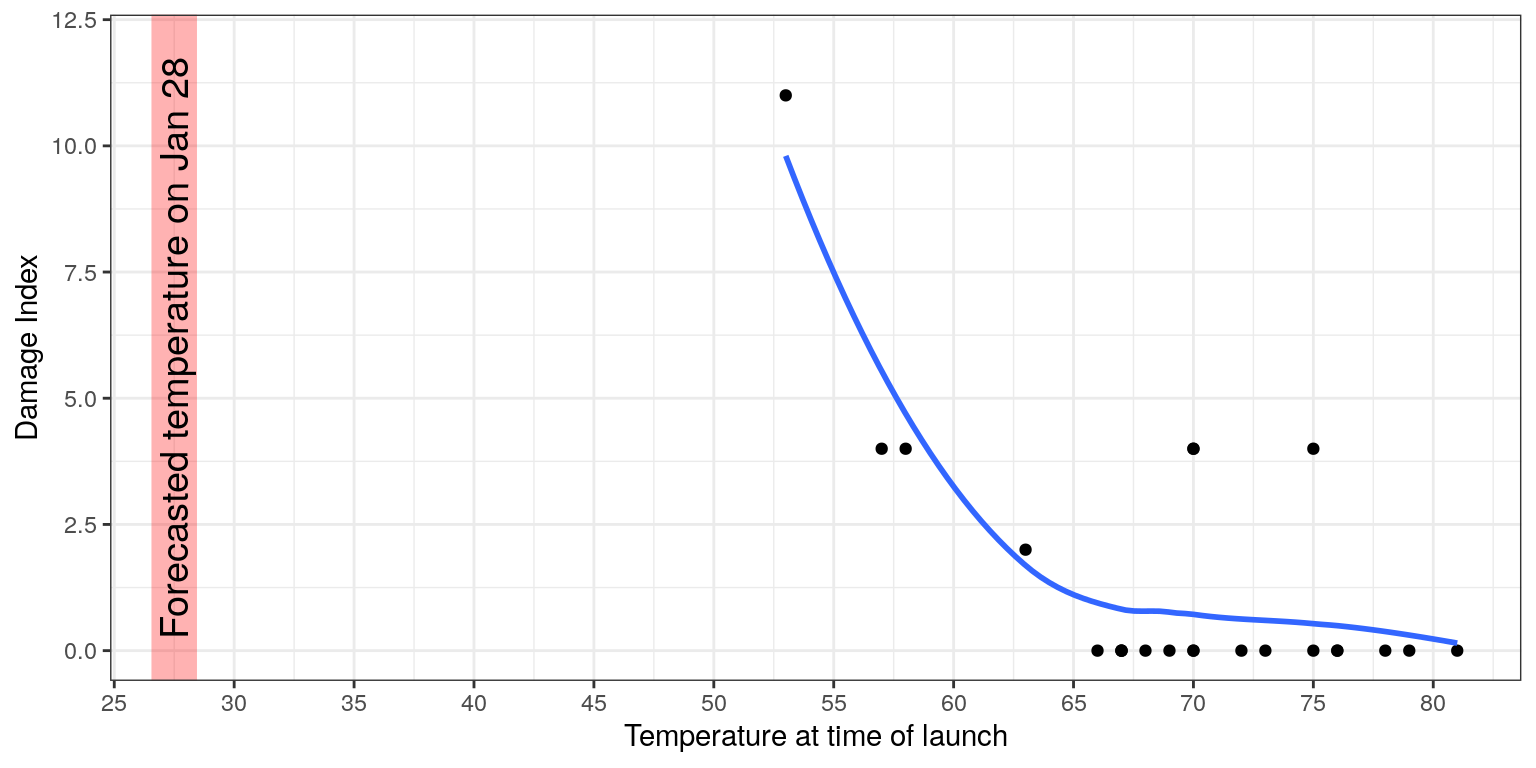
\includegraphics[height=0.5\textheight]{StatsThinking21_files/figure-latex/unnamed-chunk-67-1}

\hypertarget{additional-reading-and-resources}{%
\section{Additional reading and resources}\label{additional-reading-and-resources}}

\begin{itemize}
\item
  \href{http://ggplot2.tidyverse.org/reference/ggtheme.html}{ggplot theme reference}
\item
  \href{http://www.ggplot2-exts.org/ggtech.html}{knockoff tech themes}
\end{itemize}

\hypertarget{fitting-simple-models-with-r}{%
\chapter{Fitting simple models with R}\label{fitting-simple-models-with-r}}

In this chapter we will focus on how to compute the measures of central tendency and variability that were covered in the previous chapter. Most of these can be computed using a built-in R function, but we will show how to do them manually in order to give some intuition about how they work.

\hypertarget{mean}{%
\section{Mean}\label{mean}}

The mean is defined as the sum of values divided by the number of values being summed:

\[
\bar{X} = \frac{\sum_{i=1}^{n}x_i}{n}
\]

Let's say that we want to obtain the mean height for adults in the NHANES database (contained in the data \texttt{Height}). We would sum the individual heights (using the \texttt{sum()} function) and then divide by the number of values:

\begin{Shaded}
\begin{Highlighting}[]
\KeywordTok{sum}\NormalTok{(NHANES}\OperatorTok{$}\NormalTok{Height)}\OperatorTok{/}\KeywordTok{length}\NormalTok{(NHANES}\OperatorTok{$}\NormalTok{Height)}
\end{Highlighting}
\end{Shaded}

\begin{verbatim}
## [1] NA
\end{verbatim}

This returns the value NA, because there are missing values for some rows, and the \texttt{sum()} function doesn't automatically handle those. To address this, we could filter the data frame using \texttt{drop\_na()} to drop rows with NA values for this variable:

\begin{Shaded}
\begin{Highlighting}[]
\NormalTok{height_noNA <-}\StringTok{ }\NormalTok{NHANES }\OperatorTok
\StringTok{  }\KeywordTok{drop_na}\NormalTok{(Height) }\OperatorTok
\StringTok{  }\KeywordTok{pull}\NormalTok{(Height)}

\KeywordTok{sum}\NormalTok{(height_noNA)}\OperatorTok{/}\KeywordTok{length}\NormalTok{(height_noNA)}
\end{Highlighting}
\end{Shaded}

\begin{verbatim}
## [1] 160.3516
\end{verbatim}

There is, of course, a built-in function in R called \texttt{mean()} that will compute the mean. Like the \texttt{sum()} function, \texttt{mean()} will return NA if there are any NA values in the data:

\begin{Shaded}
\begin{Highlighting}[]
\KeywordTok{mean}\NormalTok{(NHANES}\OperatorTok{$}\NormalTok{Height)}
\end{Highlighting}
\end{Shaded}

\begin{verbatim}
## [1] NA
\end{verbatim}

The \texttt{mean()} function includes an optional argument called \texttt{na.rm} that will remove NA values if it is set to TRUE:

\begin{Shaded}
\begin{Highlighting}[]
\KeywordTok{mean}\NormalTok{(NHANES}\OperatorTok{$}\NormalTok{Height, }\DataTypeTok{na.rm=}\OtherTok{TRUE}\NormalTok{)}
\end{Highlighting}
\end{Shaded}

\begin{verbatim}
## [1] 160.3516
\end{verbatim}

\hypertarget{median}{%
\section{Median}\label{median}}

The median is the middle value after sorting the entire set of values. Let's use the cleand-up \texttt{height\_noNA} variable created above to determine this for the NHANES height data. First we sort the data in order of their values:

\begin{Shaded}
\begin{Highlighting}[]
\NormalTok{height_sorted <-}\StringTok{ }\KeywordTok{sort}\NormalTok{(height_noNA)}
\end{Highlighting}
\end{Shaded}

Next we find the median value. If there is an odd number of values in the list, then this is just the value in the middle, whereas if the number of values is even then we take the average of the two middle values. We can determine whether the number of items is even by dividing the length by two and seeing if there is a remainder; we do this using the \texttt{\%\%} operator, which is known as the \emph{modulus} and returns the remainder:

\begin{Shaded}
\begin{Highlighting}[]
\DecValTok{5} \OperatorTok\StringTok{ }\DecValTok{2}
\end{Highlighting}
\end{Shaded}

\begin{verbatim}
## [1] 1
\end{verbatim}

Here we will test whether the remainder is equal to one; if it is, then we will take the middle value, otherwise we will take the average of the two middle values. We can do this using an if/else structure, which executes different processes depending on which of the arguments are true:

\begin{verbatim}
if (logical value) {
  functions to perform if logical value is true
} else {
  functions to perform if logical value is false

}
\end{verbatim}

Let's do this with our data. To find the middle value when the number of items is odd, we will divide the length and then round up, using the \texttt{ceiling()} function:

\begin{Shaded}
\begin{Highlighting}[]
\ControlFlowTok{if}\NormalTok{ (}\KeywordTok{length}\NormalTok{(height_sorted) }\OperatorTok\StringTok{ }\DecValTok{2} \OperatorTok{==}\StringTok{ }\DecValTok{1}\NormalTok{)\{}
  \CommentTok{# length of vector is odd}
\NormalTok{  median_height <-}\StringTok{ }
\StringTok{    }\NormalTok{height_sorted[}\KeywordTok{ceiling}\NormalTok{(}\KeywordTok{length}\NormalTok{(height_sorted) }\OperatorTok{/}\StringTok{ }\DecValTok{2}\NormalTok{)]}
\NormalTok{\} }\ControlFlowTok{else}\NormalTok{ \{}
\NormalTok{  median_height <-}\StringTok{ }
\StringTok{    }\NormalTok{(height_sorted[}\KeywordTok{length}\NormalTok{(height_sorted) }\OperatorTok{/}\StringTok{ }\DecValTok{2}\NormalTok{] }\OperatorTok{+}\StringTok{ }
\StringTok{        }\NormalTok{height_sorted[}\DecValTok{1} \OperatorTok{+}\StringTok{ }\KeywordTok{length}\NormalTok{(height_sorted) }\OperatorTok{/}\StringTok{ }\NormalTok{(}\DecValTok{2}\NormalTok{)])}\OperatorTok{/}\DecValTok{2}
\NormalTok{\}}

\NormalTok{median_height}
\end{Highlighting}
\end{Shaded}

\begin{verbatim}
## [1] 165.1
\end{verbatim}

We can compare this to the result from the built-in median function:

\begin{Shaded}
\begin{Highlighting}[]
\KeywordTok{median}\NormalTok{(height_noNA)}
\end{Highlighting}
\end{Shaded}

\begin{verbatim}
## [1] 165.1
\end{verbatim}

\hypertarget{mode}{%
\section{Mode}\label{mode}}

The mode is the most frequent value that occurs in a variable. R has a function called \texttt{mode()} but if you look at the help page you will see that it doesn't actually copute the mode. In fact, R doesn't have a built-in function to compute the mode, so we need to create one. Let start with some toy data:

\begin{Shaded}
\begin{Highlighting}[]
\NormalTok{mode_test =}\StringTok{ }\KeywordTok{c}\NormalTok{(}\StringTok{'a'}\NormalTok{, }\StringTok{'b'}\NormalTok{, }\StringTok{'b'}\NormalTok{, }\StringTok{'c'}\NormalTok{, }\StringTok{'c'}\NormalTok{, }\StringTok{'c'}\NormalTok{)}
\NormalTok{mode_test}
\end{Highlighting}
\end{Shaded}

\begin{verbatim}
## [1] "a" "b" "b" "c" "c" "c"
\end{verbatim}

We can see by eye that the mode is ``a'' since it occurs more often than the others. To find it computationally, let's first get the unique values

To do this, we first create a table with the counts for each value, using the \texttt{table()} function:

\begin{Shaded}
\begin{Highlighting}[]
\NormalTok{mode_table <-}\StringTok{ }\KeywordTok{table}\NormalTok{(mode_test)}
\NormalTok{mode_table}
\end{Highlighting}
\end{Shaded}

\begin{verbatim}
## mode_test
## a b c 
## 1 2 3
\end{verbatim}

Now we need to find the maximum value. We do this by comparing each value to the maximum of the table; this will work even if there are multiple values with the same frequency (i.e.~a tie for the mode).

\begin{Shaded}
\begin{Highlighting}[]
\NormalTok{table_max <-}\StringTok{ }\NormalTok{mode_table[mode_table }\OperatorTok{==}\StringTok{ }\KeywordTok{max}\NormalTok{(mode_table)]}
\NormalTok{table_max}
\end{Highlighting}
\end{Shaded}

\begin{verbatim}
## c 
## 3
\end{verbatim}

This variable is a special kind of value called a \emph{named vector}, and its name contains the value that we need to identify the mode. We can pull it out using the \texttt{names()} function:

\begin{Shaded}
\begin{Highlighting}[]
\NormalTok{my_mode <-}\StringTok{ }\KeywordTok{names}\NormalTok{(table_max)[}\DecValTok{1}\NormalTok{]}
\NormalTok{my_mode}
\end{Highlighting}
\end{Shaded}

\begin{verbatim}
## [1] "c"
\end{verbatim}

Let's wrap this up into our own custom function:

\begin{Shaded}
\begin{Highlighting}[]
\NormalTok{getmode <-}\StringTok{ }\ControlFlowTok{function}\NormalTok{(v, }\DataTypeTok{print_table=}\OtherTok{FALSE}\NormalTok{) \{}
\NormalTok{  mode_table <-}\StringTok{ }\KeywordTok{table}\NormalTok{(v)}
  \ControlFlowTok{if}\NormalTok{ (print_table)\{}
    \KeywordTok{print}\NormalTok{(}\KeywordTok{kable}\NormalTok{(mode_table))}
\NormalTok{  \}}
\NormalTok{  table_max <-}\StringTok{ }\NormalTok{mode_table[mode_table }\OperatorTok{==}\StringTok{ }\KeywordTok{max}\NormalTok{(mode_table)]}
  \KeywordTok{return}\NormalTok{(}\KeywordTok{names}\NormalTok{(table_max))}
\NormalTok{\}}
\end{Highlighting}
\end{Shaded}

We can then apply this to real data. Let's apply this to the \texttt{MaritalStatus} variable in the NHANES dataset:

\begin{Shaded}
\begin{Highlighting}[]
\KeywordTok{getmode}\NormalTok{(NHANES}\OperatorTok{$}\NormalTok{MaritalStatus)}
\end{Highlighting}
\end{Shaded}

\begin{verbatim}
## [1] "Married"
\end{verbatim}

\hypertarget{variability}{%
\section{Variability}\label{variability}}

Let's first compute the \emph{variance}, which is the average squared difference between each value and the mean. Let's do this with our cleaned-up version of the height data, but instead of working with the entire dataset, let's take a random sample of 150 individuals:

\begin{Shaded}
\begin{Highlighting}[]
\NormalTok{height_sample <-}\StringTok{ }\NormalTok{NHANES }\OperatorTok
\StringTok{  }\KeywordTok{drop_na}\NormalTok{(Height) }\OperatorTok
\StringTok{  }\KeywordTok{sample_n}\NormalTok{(}\DecValTok{150}\NormalTok{) }\OperatorTok
\StringTok{  }\KeywordTok{pull}\NormalTok{(Height)}
\end{Highlighting}
\end{Shaded}

First we need to obtain the sum of squared errors from the mean. In R, we can square a vector using \texttt{**2}:

\begin{Shaded}
\begin{Highlighting}[]
\NormalTok{SSE <-}\StringTok{ }\KeywordTok{sum}\NormalTok{((height_sample }\OperatorTok{-}\StringTok{ }\KeywordTok{mean}\NormalTok{(height_sample))}\OperatorTok{**}\DecValTok{2}\NormalTok{)}
\NormalTok{SSE}
\end{Highlighting}
\end{Shaded}

\begin{verbatim}
## [1] 63419.37
\end{verbatim}

Then we divide by N - 1 to get the estimated variance:

\begin{Shaded}
\begin{Highlighting}[]
\NormalTok{var_est <-}\StringTok{ }\NormalTok{SSE}\OperatorTok{/}\NormalTok{(}\KeywordTok{length}\NormalTok{(height_sample) }\OperatorTok{-}\StringTok{ }\DecValTok{1}\NormalTok{)}
\NormalTok{var_est}
\end{Highlighting}
\end{Shaded}

\begin{verbatim}
## [1] 425.6333
\end{verbatim}

We can compare this to the built-in \texttt{var()} function:

\begin{Shaded}
\begin{Highlighting}[]
\KeywordTok{var}\NormalTok{(height_sample)}
\end{Highlighting}
\end{Shaded}

\begin{verbatim}
## [1] 425.6333
\end{verbatim}

We can get the \emph{standard deviation} by simply taking the square root of the variance:

\begin{Shaded}
\begin{Highlighting}[]
\KeywordTok{sqrt}\NormalTok{(var_est)}
\end{Highlighting}
\end{Shaded}

\begin{verbatim}
## [1] 20.63088
\end{verbatim}

Which is the same value obtained using the built-in \texttt{sd()} function:

\begin{Shaded}
\begin{Highlighting}[]
\KeywordTok{sd}\NormalTok{(height_sample)}
\end{Highlighting}
\end{Shaded}

\begin{verbatim}
## [1] 20.63088
\end{verbatim}

\hypertarget{z-scores}{%
\section{Z-scores}\label{z-scores}}

A Z-score is obtained by first subtracting the mean and then dividing by the standard deviation of a distribution. Let's do this for the \texttt{height\_sample} data.

\begin{Shaded}
\begin{Highlighting}[]
\NormalTok{mean_height <-}\StringTok{ }\KeywordTok{mean}\NormalTok{(height_sample)}
\NormalTok{sd_height <-}\StringTok{ }\KeywordTok{sd}\NormalTok{(height_sample)}

\NormalTok{z_height <-}\StringTok{ }\NormalTok{(height_sample }\OperatorTok{-}\StringTok{ }\NormalTok{mean_height)}\OperatorTok{/}\NormalTok{sd_height}
\end{Highlighting}
\end{Shaded}

Now let's plot the histogram of Z-scores alongside the histogram for the original values. We will use the \texttt{plot\_grid()} function from the \texttt{cowplot} library to plot the two figures alongside one another. First we need to put the values into a data frame, since \texttt{ggplot()} requires the data to be contained in a data frame.

\begin{Shaded}
\begin{Highlighting}[]
\NormalTok{height_df <-}\StringTok{ }\KeywordTok{data.frame}\NormalTok{(}\DataTypeTok{orig_height=}\NormalTok{height_sample, }
                        \DataTypeTok{z_height=}\NormalTok{z_height)}

\CommentTok{# create individual plots}
\NormalTok{plot_orig <-}\StringTok{ }\KeywordTok{ggplot}\NormalTok{(height_df, }\KeywordTok{aes}\NormalTok{(orig_height)) }\OperatorTok{+}\StringTok{ }
\StringTok{  }\KeywordTok{geom_histogram}\NormalTok{()}
\NormalTok{plot_z <-}\StringTok{ }\KeywordTok{ggplot}\NormalTok{(height_df, }\KeywordTok{aes}\NormalTok{(z_height)) }\OperatorTok{+}\StringTok{ }
\StringTok{  }\KeywordTok{geom_histogram}\NormalTok{()}

\CommentTok{# combine into a single figure}
\KeywordTok{plot_grid}\NormalTok{(plot_orig, plot_z)}
\end{Highlighting}
\end{Shaded}

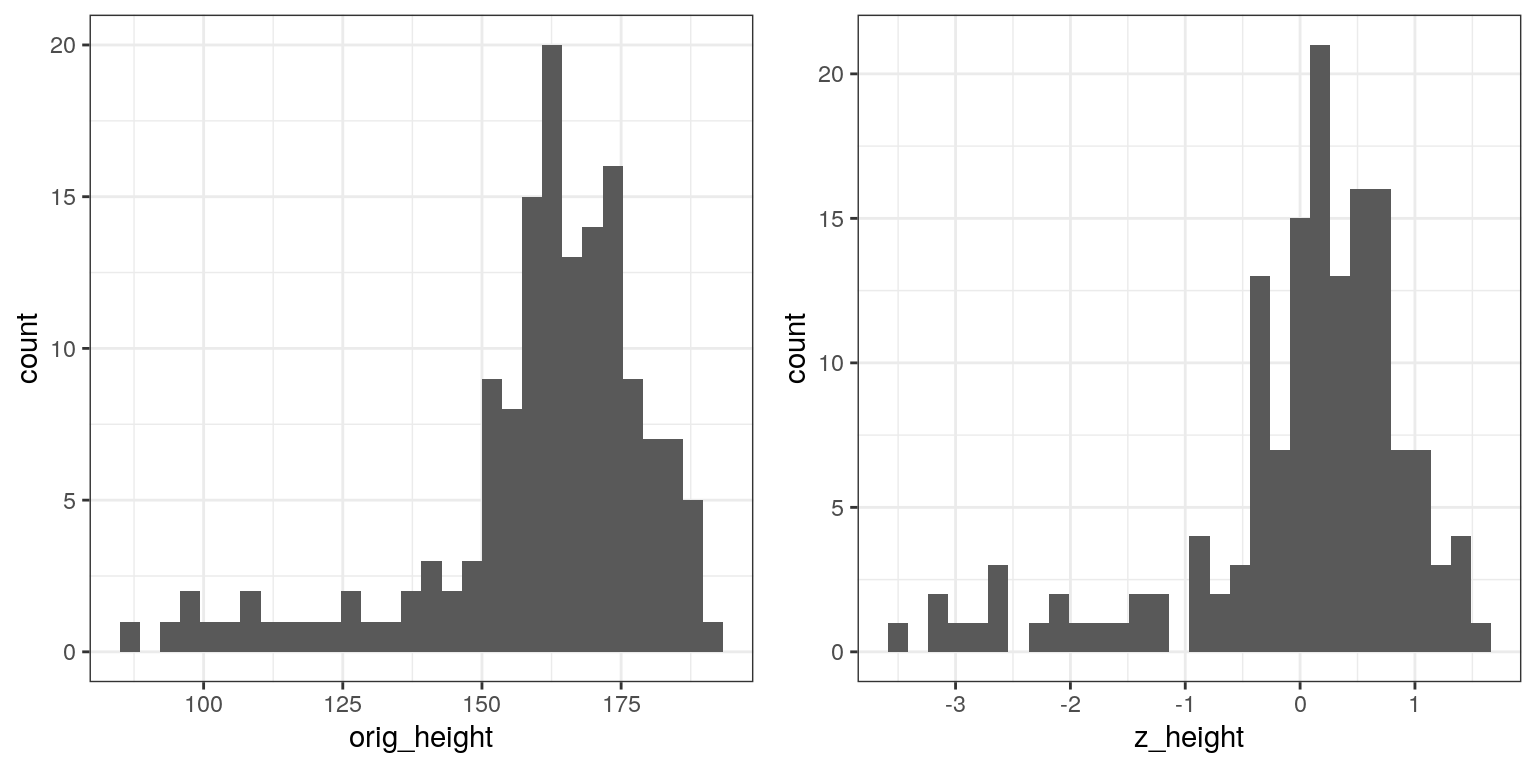
\includegraphics{StatsThinking21_files/figure-latex/unnamed-chunk-90-1.pdf}

You will notice that the shapes of the histograms are similar but not exactly the same. This occurs because the binning is slightly different between the two sets of values. However, if we plot them against one another in a scatterplot, we will see that there is a direct linear relation between the two sets of values:

\begin{Shaded}
\begin{Highlighting}[]
\KeywordTok{ggplot}\NormalTok{(height_df, }\KeywordTok{aes}\NormalTok{(orig_height, z_height)) }\OperatorTok{+}\StringTok{ }
\StringTok{  }\KeywordTok{geom_point}\NormalTok{()}
\end{Highlighting}
\end{Shaded}

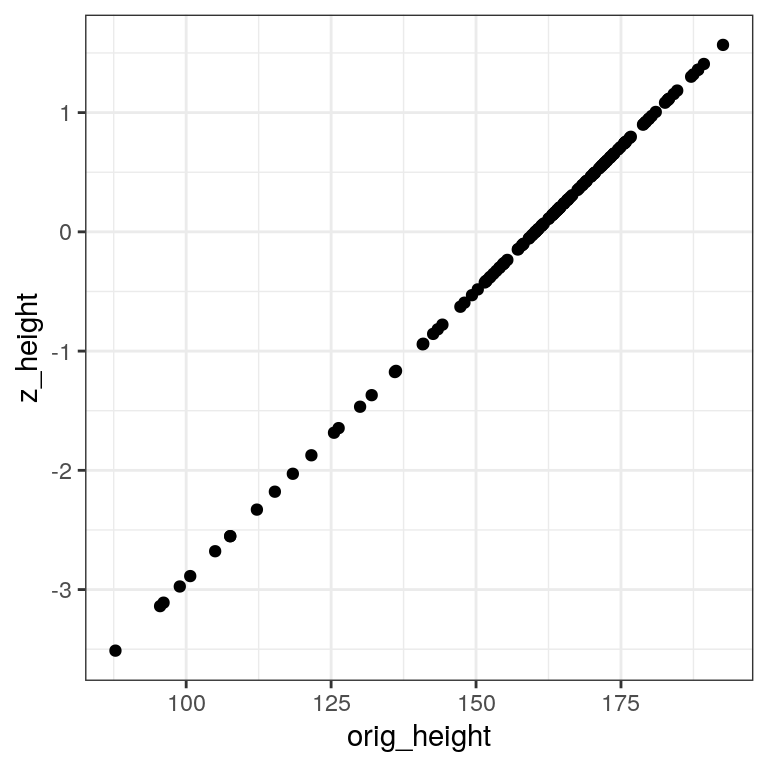
\includegraphics{StatsThinking21_files/figure-latex/unnamed-chunk-91-1.pdf}

\hypertarget{probability-in-r-with-lucy-king}{%
\chapter{Probability in R (with Lucy King)}\label{probability-in-r-with-lucy-king}}

In this chapter we will go over probability computations in R.

\hypertarget{basic-probability-calculations}{%
\section{Basic probability calculations}\label{basic-probability-calculations}}

Let's create a vector of outcomes from one to 6, using the \texttt{seq()} function to create such a sequence:

\begin{Shaded}
\begin{Highlighting}[]
\NormalTok{outcomes <-}\StringTok{ }\KeywordTok{seq}\NormalTok{(}\DecValTok{1}\NormalTok{, }\DecValTok{6}\NormalTok{)}
\NormalTok{outcomes}
\end{Highlighting}
\end{Shaded}

\begin{verbatim}
## [1] 1 2 3 4 5 6
\end{verbatim}

Now let's create a vector of logical values based on whether the outcome in each position is equal to 1. Remember that \texttt{==} tests for equality of each element in a vector:

\begin{Shaded}
\begin{Highlighting}[]
\NormalTok{outcome1isTrue <-}\StringTok{ }\NormalTok{outcomes }\OperatorTok{==}\StringTok{ }\DecValTok{1} 
\NormalTok{outcome1isTrue}
\end{Highlighting}
\end{Shaded}

\begin{verbatim}
## [1]  TRUE FALSE FALSE FALSE FALSE FALSE
\end{verbatim}

Remember that the simple probability of an outcome is number of occurrences of the outcome divided by the total number of events. To compute a probability, we can take advantage of the fact that TRUE/FALSE are equivalent to 1/0 in R. The formula for the mean (sum of values divided by the number of values) is thus exactly the same as the formula for the simple probability! So, we can compute the probability of the event by simply taking the mean of the logical vector.

\begin{Shaded}
\begin{Highlighting}[]
\NormalTok{p1isTrue <-}\StringTok{ }\KeywordTok{mean}\NormalTok{(outcome1isTrue)}
\NormalTok{p1isTrue}
\end{Highlighting}
\end{Shaded}

\begin{verbatim}
## [1] 0.1666667
\end{verbatim}

\hypertarget{empirical-frequency-section-refempirical-frequency}{%
\section{Empirical frequency (Section \ref{empirical-frequency})}\label{empirical-frequency-section-refempirical-frequency}}

Let's walk through how we computed empirical frequency of rain in San Francisco.

First we load the data:

\begin{Shaded}
\begin{Highlighting}[]
\CommentTok{# we will remove the STATION and NAME variables }
\CommentTok{# since they are identical for all rows}
\NormalTok{SFrain <-}\StringTok{ }\KeywordTok{read_csv}\NormalTok{(}\StringTok{"data/SanFranciscoRain/1329219.csv"}\NormalTok{) }\OperatorTok\StringTok{ }
\StringTok{  }\NormalTok{dplyr}\OperatorTok{::}\KeywordTok{select}\NormalTok{(}\OperatorTok{-}\NormalTok{STATION, }\OperatorTok{-}\NormalTok{NAME)}
  
\KeywordTok{glimpse}\NormalTok{(SFrain)}
\end{Highlighting}
\end{Shaded}

\begin{verbatim}
## Observations: 365
## Variables: 2
## $ DATE <date> 2017-01-01, 2017-01-02, 2017-01-03, 2017-...
## $ PRCP <dbl> 0.05, 0.10, 0.40, 0.89, 0.01, 0.00, 0.82, ...
\end{verbatim}

We see that the data frame contains a variable called \texttt{PRCP} which denotes the amount of rain each day. Let's create a new variable called \texttt{rainToday} that denotes whether the amount of precipitation was above zero:

\begin{Shaded}
\begin{Highlighting}[]
\NormalTok{SFrain <-}\StringTok{ }
\StringTok{  }\NormalTok{SFrain }\OperatorTok
\StringTok{  }\KeywordTok{mutate}\NormalTok{(}\DataTypeTok{rainToday =} \KeywordTok{as.integer}\NormalTok{(PRCP }\OperatorTok{>}\StringTok{ }\DecValTok{0}\NormalTok{))}

\KeywordTok{glimpse}\NormalTok{(SFrain)}
\end{Highlighting}
\end{Shaded}

\begin{verbatim}
## Observations: 365
## Variables: 3
## $ DATE      <date> 2017-01-01, 2017-01-02, 2017-01-03, ...
## $ PRCP      <dbl> 0.05, 0.10, 0.40, 0.89, 0.01, 0.00, 0...
## $ rainToday <int> 1, 1, 1, 1, 1, 0, 1, 1, 1, 1, 1, 1, 0...
\end{verbatim}

Now we will summarize the data to compute the probability of rain:

\begin{Shaded}
\begin{Highlighting}[]
\NormalTok{pRainInSF <-}\StringTok{ }
\StringTok{  }\NormalTok{SFrain }\OperatorTok
\StringTok{  }\KeywordTok{summarize}\NormalTok{(}
    \DataTypeTok{pRainInSF =} \KeywordTok{mean}\NormalTok{(rainToday)}
\NormalTok{  ) }\OperatorTok
\StringTok{  }\KeywordTok{pull}\NormalTok{()}

\NormalTok{pRainInSF}
\end{Highlighting}
\end{Shaded}

\begin{verbatim}
## [1] 0.2
\end{verbatim}

\hypertarget{conditional-probability-section-refconditional-probability}{%
\section{Conditional probability (Section \ref{conditional-probability})}\label{conditional-probability-section-refconditional-probability}}

Let's determine the conditional probability of someone being unhealthy, given that they are over 70 years of age, using the NHANES dataset. Let's create a new data frame that only contains people over 70 years old.

\begin{Shaded}
\begin{Highlighting}[]
\NormalTok{healthDataFrame <-}
\StringTok{  }\NormalTok{NHANES }\OperatorTok
\StringTok{  }\KeywordTok{mutate}\NormalTok{(}
    \DataTypeTok{Over70 =}\NormalTok{ Age }\OperatorTok{>}\StringTok{ }\DecValTok{70}\NormalTok{,}
    \DataTypeTok{Unhealthy =}\NormalTok{ DaysPhysHlthBad }\OperatorTok{>}\StringTok{ }\DecValTok{0}
\NormalTok{  ) }\OperatorTok
\StringTok{  }\NormalTok{dplyr}\OperatorTok{::}\KeywordTok{select}\NormalTok{(Unhealthy, Over70) }\OperatorTok
\StringTok{  }\KeywordTok{drop_na}\NormalTok{()}

\KeywordTok{glimpse}\NormalTok{(healthDataFrame)}
\end{Highlighting}
\end{Shaded}

\begin{verbatim}
## Observations: 4,891
## Variables: 2
## $ Unhealthy <lgl> FALSE, FALSE, FALSE, TRUE, FALSE, TRU...
## $ Over70    <lgl> FALSE, FALSE, FALSE, FALSE, FALSE, FA...
\end{verbatim}

First, what's the probability of being over 70?

\begin{Shaded}
\begin{Highlighting}[]
\NormalTok{pOver70 <-}\StringTok{ }
\StringTok{  }\NormalTok{healthDataFrame }\OperatorTok
\StringTok{  }\KeywordTok{summarise}\NormalTok{(}\DataTypeTok{pOver70 =} \KeywordTok{mean}\NormalTok{(Over70)) }\OperatorTok\StringTok{ }
\StringTok{  }\KeywordTok{pull}\NormalTok{()}

\CommentTok{# to obtain the specific value, we need to extract it from the data frame}

\NormalTok{pOver70}
\end{Highlighting}
\end{Shaded}

\begin{verbatim}
## [1] 0.1106113
\end{verbatim}

Second, what's the probability of being unhealthy?

\begin{Shaded}
\begin{Highlighting}[]
\NormalTok{pUnhealthy <-}\StringTok{ }
\StringTok{  }\NormalTok{healthDataFrame }\OperatorTok
\StringTok{  }\KeywordTok{summarise}\NormalTok{(}\DataTypeTok{pUnhealthy =} \KeywordTok{mean}\NormalTok{(Unhealthy)) }\OperatorTok\StringTok{ }
\StringTok{  }\KeywordTok{pull}\NormalTok{()}

\NormalTok{pUnhealthy}
\end{Highlighting}
\end{Shaded}

\begin{verbatim}
## [1] 0.3567778
\end{verbatim}

What's the probability for each combination of unhealthy/healthy and over 70/ not? We can create a new variable that finds the joint probability by multiplying the two individual binary variables together; since anything times zero is zero, this will only have the value 1 for any case where both are true.

\begin{Shaded}
\begin{Highlighting}[]
\NormalTok{pBoth <-}\StringTok{ }\NormalTok{healthDataFrame }\OperatorTok\StringTok{ }
\StringTok{  }\KeywordTok{mutate}\NormalTok{(}
    \DataTypeTok{both =}\NormalTok{ Unhealthy}\OperatorTok{*}\NormalTok{Over70}
\NormalTok{  ) }\OperatorTok
\StringTok{  }\KeywordTok{summarise}\NormalTok{(}
    \DataTypeTok{pBoth =} \KeywordTok{mean}\NormalTok{(both)) }\OperatorTok\StringTok{ }
\StringTok{  }\KeywordTok{pull}\NormalTok{()}

\NormalTok{pBoth}
\end{Highlighting}
\end{Shaded}

\begin{verbatim}
## [1] 0.04252709
\end{verbatim}

Finally, what's the probability of someone being unhealthy, given that they are over 70 years of age?

\begin{Shaded}
\begin{Highlighting}[]
\NormalTok{pUnhealthyGivenOver70 <-}
\StringTok{  }\NormalTok{healthDataFrame }\OperatorTok
\StringTok{  }\KeywordTok{filter}\NormalTok{(Over70 }\OperatorTok{==}\StringTok{ }\OtherTok{TRUE}\NormalTok{) }\OperatorTok\StringTok{ }\CommentTok{# limit to Over70}
\StringTok{  }\KeywordTok{summarise}\NormalTok{(}\DataTypeTok{pUnhealthy =} \KeywordTok{mean}\NormalTok{(Unhealthy)) }\OperatorTok\StringTok{ }
\StringTok{  }\KeywordTok{pull}\NormalTok{()}

\NormalTok{pUnhealthyGivenOver70}
\end{Highlighting}
\end{Shaded}

\begin{verbatim}
## [1] 0.3844732
\end{verbatim}

\begin{Shaded}
\begin{Highlighting}[]
\CommentTok{# compute the opposite:}
\CommentTok{# what the probability of being over 70 given that }
\CommentTok{# one is unhealthy?}
\NormalTok{pOver70givenUnhealthy <-}
\StringTok{  }\NormalTok{healthDataFrame }\OperatorTok
\StringTok{  }\KeywordTok{filter}\NormalTok{(Unhealthy }\OperatorTok{==}\StringTok{ }\OtherTok{TRUE}\NormalTok{) }\OperatorTok\StringTok{ }\CommentTok{# limit to Unhealthy}
\StringTok{  }\KeywordTok{summarise}\NormalTok{(}\DataTypeTok{pOver70 =} \KeywordTok{mean}\NormalTok{(Over70)) }\OperatorTok\StringTok{ }
\StringTok{  }\KeywordTok{pull}\NormalTok{()}

\NormalTok{pOver70givenUnhealthy}
\end{Highlighting}
\end{Shaded}

\begin{verbatim}
## [1] 0.1191977
\end{verbatim}

\hypertarget{sampling-in-r}{%
\chapter{Sampling in R}\label{sampling-in-r}}

First we load the necessary libraries and set up the NHANES adult dataset

\begin{Shaded}
\begin{Highlighting}[]
\KeywordTok{library}\NormalTok{(tidyverse)}
\KeywordTok{library}\NormalTok{(ggplot2)}
\KeywordTok{library}\NormalTok{(knitr)}
\KeywordTok{library}\NormalTok{(cowplot)}

\KeywordTok{set.seed}\NormalTok{(}\DecValTok{123456}\NormalTok{)}
\NormalTok{opts_chunk}\OperatorTok{$}\KeywordTok{set}\NormalTok{(}\DataTypeTok{tidy.opts=}\KeywordTok{list}\NormalTok{(}\DataTypeTok{width.cutoff=}\DecValTok{80}\NormalTok{))}
\KeywordTok{options}\NormalTok{(}\DataTypeTok{tibble.width =} \DecValTok{60}\NormalTok{)}


\CommentTok{# load the NHANES data library}
\KeywordTok{library}\NormalTok{(NHANES)}

\CommentTok{# create a NHANES dataset without duplicated IDs }
\NormalTok{NHANES <-}
\StringTok{  }\NormalTok{NHANES }\OperatorTok
\StringTok{  }\KeywordTok{distinct}\NormalTok{(ID, }\DataTypeTok{.keep_all =} \OtherTok{TRUE}\NormalTok{) }

\CommentTok{#create a dataset of only adults}
\NormalTok{NHANES_adult <-}\StringTok{ }
\StringTok{  }\NormalTok{NHANES }\OperatorTok
\StringTok{  }\KeywordTok{filter}\NormalTok{( }
\NormalTok{    Age }\OperatorTok{>=}\StringTok{ }\DecValTok{18}
\NormalTok{  ) }\OperatorTok
\StringTok{  }\KeywordTok{drop_na}\NormalTok{(Height)}
\end{Highlighting}
\end{Shaded}

\hypertarget{sampling-error-section-refsamplingerror}{%
\section{Sampling error (Section \ref{samplingerror})}\label{sampling-error-section-refsamplingerror}}

Here we will repeatedly sample from the NHANES Height variable in order to obtain the sampling distribution of the mean.

\begin{Shaded}
\begin{Highlighting}[]
\NormalTok{sampSize <-}\StringTok{ }\DecValTok{50} \CommentTok{# size of sample}
\NormalTok{nsamps <-}\StringTok{ }\DecValTok{5000} \CommentTok{# number of samples we will take}

\CommentTok{# set up variable to store all of the results}
\NormalTok{sampMeans <-}\StringTok{ }\KeywordTok{tibble}\NormalTok{(}\DataTypeTok{meanHeight=}\KeywordTok{rep}\NormalTok{(}\OtherTok{NA}\NormalTok{,nsamps))}

\CommentTok{# Loop through and repeatedly sample and compute the mean}
\ControlFlowTok{for}\NormalTok{ (i }\ControlFlowTok{in} \DecValTok{1}\OperatorTok{:}\NormalTok{nsamps) \{}
\NormalTok{  sampMeans}\OperatorTok{$}\NormalTok{meanHeight[i] <-}\StringTok{ }\NormalTok{NHANES_adult }\OperatorTok
\StringTok{    }\KeywordTok{sample_n}\NormalTok{(sampSize) }\OperatorTok
\StringTok{    }\KeywordTok{summarize}\NormalTok{(}\DataTypeTok{meanHeight=}\KeywordTok{mean}\NormalTok{(Height)) }\OperatorTok
\StringTok{    }\KeywordTok{pull}\NormalTok{(meanHeight)}
\NormalTok{\}}
\end{Highlighting}
\end{Shaded}

Now let's plot the sampling distribution. We will also overlay the sampling distribution of the mean predicted on the basis of the population mean and standard deviation, to show that it properly describes the actual sampling distribution.

\begin{Shaded}
\begin{Highlighting}[]
\CommentTok{# pipe the sampMeans data frame into ggplot}
\NormalTok{sampMeans }\OperatorTok\StringTok{ }
\StringTok{  }\KeywordTok{ggplot}\NormalTok{(}\KeywordTok{aes}\NormalTok{(meanHeight)) }\OperatorTok{+}
\StringTok{  }\CommentTok{# create histogram using density rather than count}
\StringTok{  }\KeywordTok{geom_histogram}\NormalTok{(}
    \KeywordTok{aes}\NormalTok{(}\DataTypeTok{y =}\NormalTok{ ..density..),}
    \DataTypeTok{bins =} \DecValTok{50}\NormalTok{,}
    \DataTypeTok{col =} \StringTok{"gray"}\NormalTok{, }
    \DataTypeTok{fill =} \StringTok{"gray"}
\NormalTok{  ) }\OperatorTok{+}
\StringTok{  }\CommentTok{# add a vertical line for the population mean}
\StringTok{  }\KeywordTok{geom_vline}\NormalTok{(}\DataTypeTok{xintercept =} \KeywordTok{mean}\NormalTok{(NHANES_adult}\OperatorTok{$}\NormalTok{Height),}
             \DataTypeTok{size=}\FloatTok{1.5}\NormalTok{) }\OperatorTok{+}
\StringTok{  }\CommentTok{# add a label for the line}
\StringTok{  }\KeywordTok{annotate}\NormalTok{(}
    \StringTok{"text"}\NormalTok{,}
    \DataTypeTok{x =} \FloatTok{169.6}\NormalTok{, }
    \DataTypeTok{y =} \FloatTok{.4}\NormalTok{,}
    \DataTypeTok{label =} \StringTok{"Population mean"}\NormalTok{,}
    \DataTypeTok{size=}\DecValTok{6}
\NormalTok{  ) }\OperatorTok{+}
\StringTok{  }\CommentTok{# label the x axis}
\StringTok{  }\KeywordTok{labs}\NormalTok{(}\DataTypeTok{x =} \StringTok{"Height (cm)"}\NormalTok{) }\OperatorTok{+}
\StringTok{  }\CommentTok{# add normal based on population mean/sd}
\StringTok{  }\KeywordTok{stat_function}\NormalTok{(}
      \DataTypeTok{fun =}\NormalTok{ dnorm, }\DataTypeTok{n =}\NormalTok{ sampSize,}
      \DataTypeTok{args =} \KeywordTok{list}\NormalTok{(}
        \DataTypeTok{mean =} \KeywordTok{mean}\NormalTok{(NHANES_adult}\OperatorTok{$}\NormalTok{Height),}
        \DataTypeTok{sd =} \KeywordTok{sd}\NormalTok{(NHANES_adult}\OperatorTok{$}\NormalTok{Height)}\OperatorTok{/}\KeywordTok{sqrt}\NormalTok{(sampSize)}
\NormalTok{      ), }
      \DataTypeTok{size =} \FloatTok{1.5}\NormalTok{,}
      \DataTypeTok{color =} \StringTok{"black"}\NormalTok{,}
      \DataTypeTok{linetype=}\StringTok{'dotted'}
\NormalTok{    ) }
\end{Highlighting}
\end{Shaded}

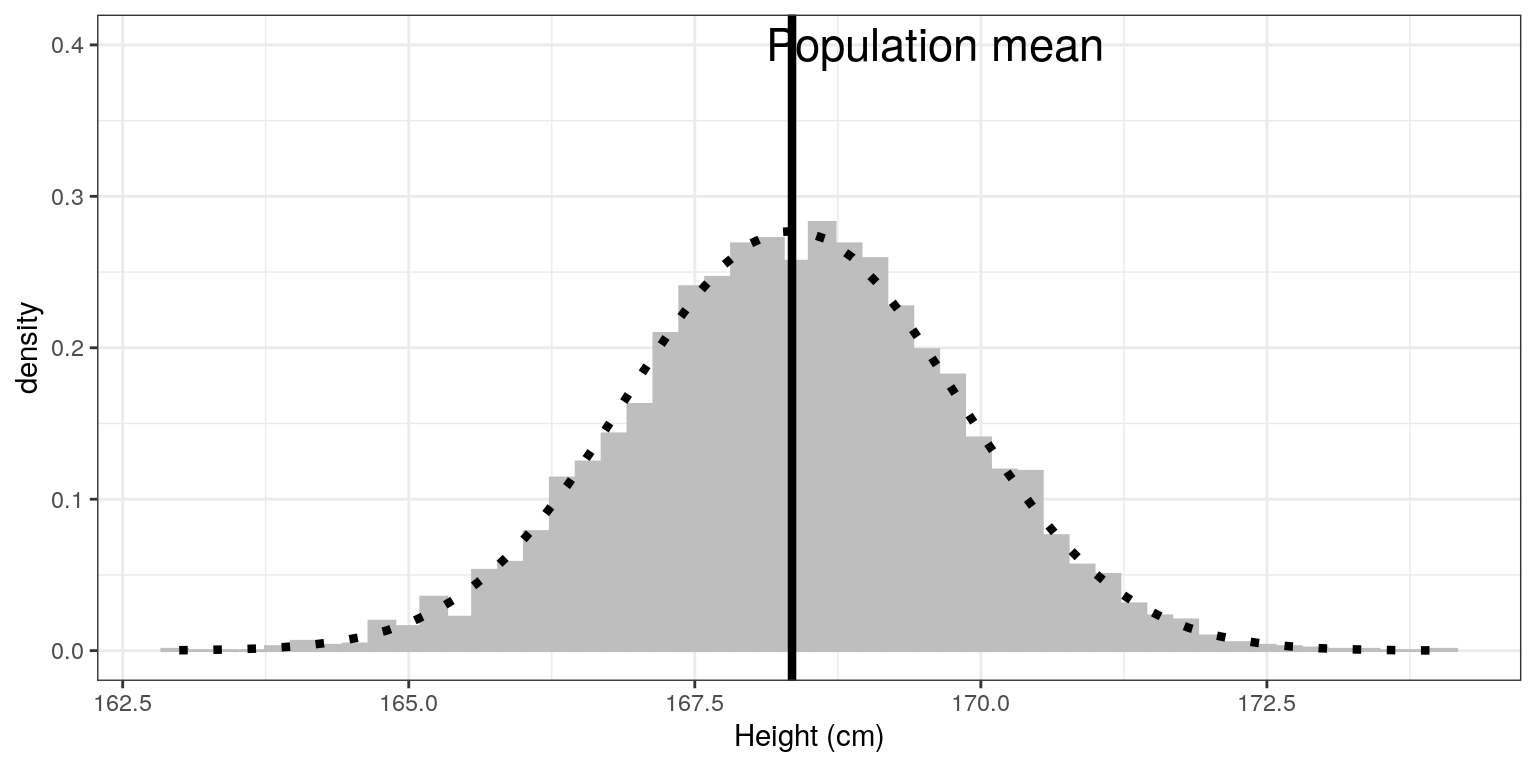
\includegraphics[height=0.5\textheight]{StatsThinking21_files/figure-latex/unnamed-chunk-107-1}

\hypertarget{central-limit-theorem}{%
\section{Central limit theorem}\label{central-limit-theorem}}

The central limit theorem tells us that the sampling distribution of the mean becomes normal as the sample size grows. Let's test this by sampling a clearly non-normal variable and look at the normality of the results using a Q-Q plot. We saw in Figure \ref{fig:alcDist50} that the variable \texttt{AlcoholYear} is distributed in a very non-normal way. Let's first look at the Q-Q plot for these data, to see what it looks like. We will use the \texttt{stat\_qq()} function from \texttt{ggplot2} to create the plot for us.

\begin{Shaded}
\begin{Highlighting}[]
\CommentTok{# prepare the dta}
\NormalTok{NHANES_cleanAlc <-}\StringTok{ }\NormalTok{NHANES }\OperatorTok
\StringTok{  }\KeywordTok{drop_na}\NormalTok{(AlcoholYear)}

\KeywordTok{ggplot}\NormalTok{(NHANES_cleanAlc, }\KeywordTok{aes}\NormalTok{(}\DataTypeTok{sample=}\NormalTok{AlcoholYear)) }\OperatorTok{+}
\StringTok{  }\KeywordTok{stat_qq}\NormalTok{() }\OperatorTok{+}\StringTok{ }
\StringTok{  }\CommentTok{# add the line for x=y}
\StringTok{  }\KeywordTok{stat_qq_line}\NormalTok{()}
\end{Highlighting}
\end{Shaded}

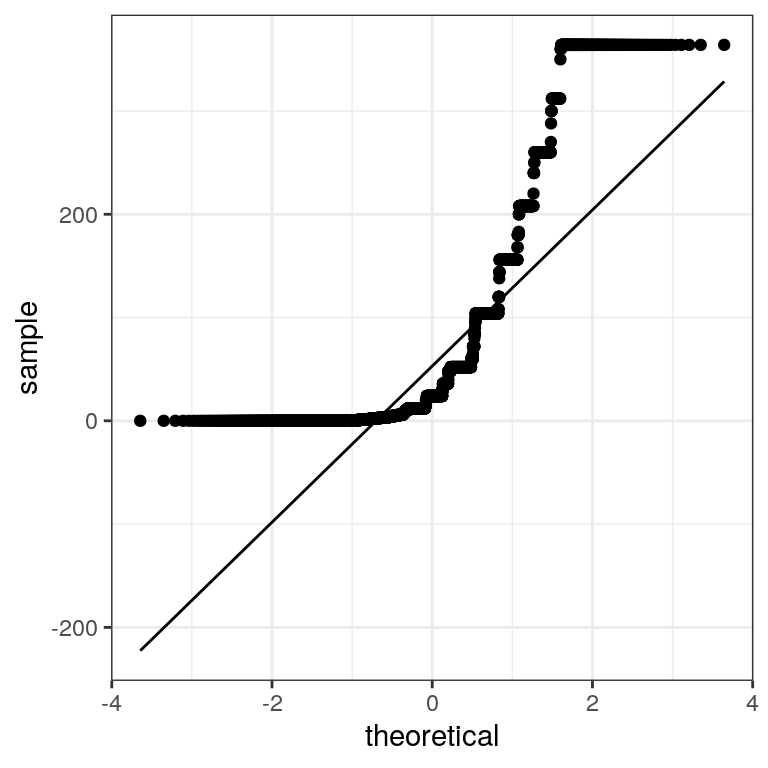
\includegraphics{StatsThinking21_files/figure-latex/unnamed-chunk-108-1.pdf}

We can see from this figure that the distribution is highly non-normal, as the Q-Q plot diverges substantially from the unit line.

Now let's repeatedly sample and compute the mean, and look at the resulting Q-Q plot. We will take samples of various sizes to see the effect of sample size. We will use a function from the \texttt{dplyr} package called \texttt{do()}, which can run a large number of analyses at once.

\begin{Shaded}
\begin{Highlighting}[]
\KeywordTok{set.seed}\NormalTok{(}\DecValTok{12345}\NormalTok{)}

\NormalTok{sampSizes <-}\StringTok{ }\KeywordTok{c}\NormalTok{(}\DecValTok{16}\NormalTok{, }\DecValTok{32}\NormalTok{, }\DecValTok{64}\NormalTok{, }\DecValTok{128}\NormalTok{) }\CommentTok{# size of sample}
\NormalTok{nsamps <-}\StringTok{ }\DecValTok{1000} \CommentTok{# number of samples we will take}

\CommentTok{# create the data frame that specifies the analyses}
\NormalTok{input_df <-}\StringTok{ }\KeywordTok{tibble}\NormalTok{(}\DataTypeTok{sampSize=}\KeywordTok{rep}\NormalTok{(sampSizes,nsamps),}
                      \DataTypeTok{id=}\KeywordTok{seq}\NormalTok{(nsamps}\OperatorTok{*}\KeywordTok{length}\NormalTok{(sampSizes)))}


\CommentTok{# create a function that samples and returns the mean}
\CommentTok{# so that we can loop over it using replicate()}
\NormalTok{get_sample_mean <-}\StringTok{ }\ControlFlowTok{function}\NormalTok{(sampSize)\{}
\NormalTok{  meanAlcYear <-}\StringTok{ }
\StringTok{    }\NormalTok{NHANES_cleanAlc }\OperatorTok
\StringTok{    }\KeywordTok{sample_n}\NormalTok{(sampSize) }\OperatorTok
\StringTok{    }\KeywordTok{summarize}\NormalTok{(}\DataTypeTok{meanAlcoholYear =} \KeywordTok{mean}\NormalTok{(AlcoholYear)) }\OperatorTok
\StringTok{    }\KeywordTok{pull}\NormalTok{(meanAlcoholYear)}
  \KeywordTok{return}\NormalTok{(}\KeywordTok{tibble}\NormalTok{(}\DataTypeTok{meanAlcYear =}\NormalTok{ meanAlcYear, }\DataTypeTok{sampSize=}\NormalTok{sampSize))}
\NormalTok{\}}

\CommentTok{# loop through sample sizes}
\CommentTok{# we group by id so that each id will be run separately by do()}
\NormalTok{all_results =}\StringTok{ }\NormalTok{input_df }\OperatorTok\StringTok{ }
\StringTok{  }\KeywordTok{group_by}\NormalTok{(id) }\OperatorTok
\StringTok{  }\CommentTok{# "." refers to the data frame being passed in by do()}
\StringTok{  }\KeywordTok{do}\NormalTok{(}\KeywordTok{get_sample_mean}\NormalTok{(.}\OperatorTok{$}\NormalTok{sampSize))}
\end{Highlighting}
\end{Shaded}

Now let's create separate Q-Q plots for the different sample sizes.

\begin{Shaded}
\begin{Highlighting}[]
\CommentTok{# create empty list to store plots}

\NormalTok{qqplots =}\StringTok{ }\KeywordTok{list}\NormalTok{()}

\ControlFlowTok{for}\NormalTok{ (N }\ControlFlowTok{in}\NormalTok{ sampSizes)\{}
\NormalTok{  sample_results <-}\StringTok{ }
\StringTok{    }\NormalTok{all_results }\OperatorTok
\StringTok{    }\KeywordTok{filter}\NormalTok{(sampSize}\OperatorTok{==}\NormalTok{N)}

\NormalTok{  qqplots[[}\KeywordTok{toString}\NormalTok{(N)]] <-}\StringTok{ }\KeywordTok{ggplot}\NormalTok{(sample_results, }
                                \KeywordTok{aes}\NormalTok{(}\DataTypeTok{sample=}\NormalTok{meanAlcYear)) }\OperatorTok{+}
\StringTok{    }\KeywordTok{stat_qq}\NormalTok{() }\OperatorTok{+}\StringTok{ }
\StringTok{    }\CommentTok{# add the line for x=y}
\StringTok{    }\KeywordTok{stat_qq_line}\NormalTok{(}\DataTypeTok{fullrange =} \OtherTok{TRUE}\NormalTok{) }\OperatorTok{+}\StringTok{ }
\StringTok{    }\KeywordTok{ggtitle}\NormalTok{(}\KeywordTok{sprintf}\NormalTok{(}\StringTok{'N = %d'}\NormalTok{, N)) }\OperatorTok{+}\StringTok{ }
\StringTok{   }\KeywordTok{xlim}\NormalTok{(}\OperatorTok{-}\DecValTok{4}\NormalTok{, }\DecValTok{4}\NormalTok{) }

\NormalTok{\}}

\KeywordTok{plot_grid}\NormalTok{(}\DataTypeTok{plotlist =}\NormalTok{ qqplots)}
\end{Highlighting}
\end{Shaded}

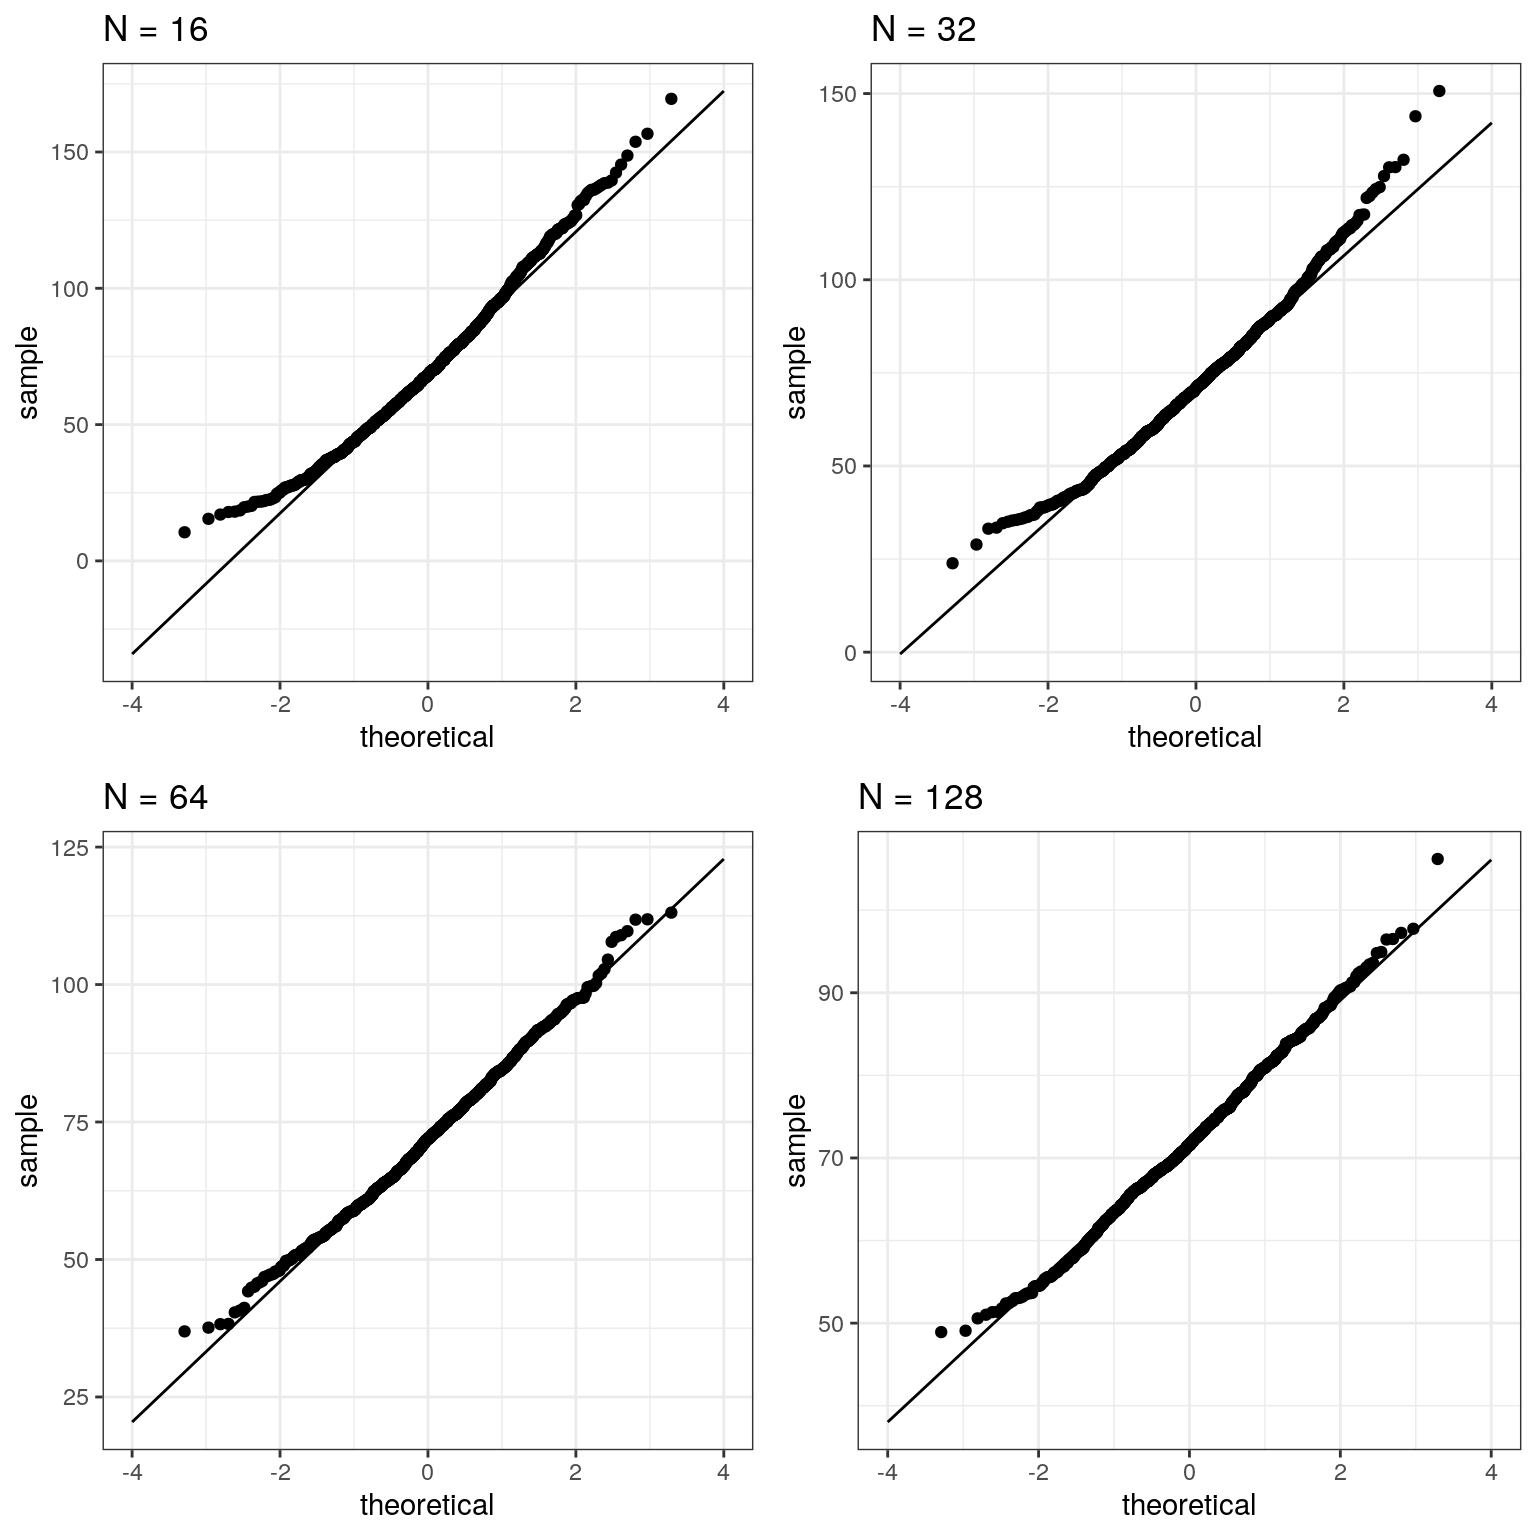
\includegraphics{StatsThinking21_files/figure-latex/unnamed-chunk-110-1.pdf}

This shows that the results become more normally distributed (i.e.~following the straight line) as the samples get larger.

\hypertarget{confidence-intervals-section-refconfidence-intervals}{%
\section{Confidence intervals (Section \ref{confidence-intervals})}\label{confidence-intervals-section-refconfidence-intervals}}

Remember that confidence intervals are intervals that will contain the population parameter on a certain proportion of times. In this example we will walk through the simulation that was presented in Section \ref{confidence-intervals} to show that this actually works properly. Here we will use a function called \texttt{do()} that lets us

\hypertarget{resampling-and-simulation-in-r}{%
\chapter{Resampling and simulation in R}\label{resampling-and-simulation-in-r}}

\hypertarget{generating-random-samples-section-refgenerating-random-numbers}{%
\section{Generating random samples (Section \ref{generating-random-numbers})}\label{generating-random-samples-section-refgenerating-random-numbers}}

Here we will generate random samples from a number of different distributions and plot their histograms.

\begin{Shaded}
\begin{Highlighting}[]
\NormalTok{nsamples <-}\StringTok{ }\DecValTok{10000}
\NormalTok{nhistbins <-}\StringTok{ }\DecValTok{100}

\CommentTok{# uniform distribution}

\NormalTok{p1 <-}
\StringTok{  }\KeywordTok{tibble}\NormalTok{(}
    \DataTypeTok{x =} \KeywordTok{runif}\NormalTok{(nsamples)}
\NormalTok{  ) }\OperatorTok\StringTok{ }
\StringTok{  }\KeywordTok{ggplot}\NormalTok{((}\KeywordTok{aes}\NormalTok{(x))) }\OperatorTok{+}
\StringTok{  }\KeywordTok{geom_histogram}\NormalTok{(}\DataTypeTok{bins =}\NormalTok{ nhistbins) }\OperatorTok{+}\StringTok{ }
\StringTok{  }\KeywordTok{labs}\NormalTok{(}\DataTypeTok{title =} \StringTok{"Uniform"}\NormalTok{)}

\CommentTok{# normal distribution}
\NormalTok{p2 <-}
\StringTok{  }\KeywordTok{tibble}\NormalTok{(}
    \DataTypeTok{x =} \KeywordTok{rnorm}\NormalTok{(nsamples)}
\NormalTok{  ) }\OperatorTok\StringTok{ }
\StringTok{  }\KeywordTok{ggplot}\NormalTok{(}\KeywordTok{aes}\NormalTok{(x)) }\OperatorTok{+}
\StringTok{  }\KeywordTok{geom_histogram}\NormalTok{(}\DataTypeTok{bins =}\NormalTok{ nhistbins) }\OperatorTok{+}
\StringTok{  }\KeywordTok{labs}\NormalTok{(}\DataTypeTok{title =} \StringTok{"Normal"}\NormalTok{)}

\CommentTok{# Chi-squared distribution}
\NormalTok{p3 <-}
\StringTok{  }\KeywordTok{tibble}\NormalTok{(}
    \DataTypeTok{x =} \KeywordTok{rnorm}\NormalTok{(nsamples)}
\NormalTok{  ) }\OperatorTok\StringTok{ }
\StringTok{  }\KeywordTok{ggplot}\NormalTok{(}\KeywordTok{aes}\NormalTok{(x)) }\OperatorTok{+}
\StringTok{  }\KeywordTok{geom_histogram}\NormalTok{(}\DataTypeTok{bins =}\NormalTok{ nhistbins) }\OperatorTok{+}
\StringTok{  }\KeywordTok{labs}\NormalTok{(}\DataTypeTok{title =} \StringTok{"Normal"}\NormalTok{)}

\CommentTok{# Chi-squared distribution}
\NormalTok{p3 <-}
\StringTok{  }\KeywordTok{tibble}\NormalTok{(}
    \DataTypeTok{x =} \KeywordTok{rchisq}\NormalTok{(nsamples, }\DataTypeTok{df=}\DecValTok{1}\NormalTok{)}
\NormalTok{  ) }\OperatorTok\StringTok{ }
\StringTok{  }\KeywordTok{ggplot}\NormalTok{(}\KeywordTok{aes}\NormalTok{(x)) }\OperatorTok{+}
\StringTok{  }\KeywordTok{geom_histogram}\NormalTok{(}\DataTypeTok{bins =}\NormalTok{ nhistbins) }\OperatorTok{+}
\StringTok{  }\KeywordTok{labs}\NormalTok{(}\DataTypeTok{title =} \StringTok{"Chi-squared"}\NormalTok{)}

\CommentTok{# Poisson distribution}
\NormalTok{p4 <-}
\StringTok{  }\KeywordTok{tibble}\NormalTok{(}
    \DataTypeTok{x =} \KeywordTok{rbinom}\NormalTok{(nsamples, }\DecValTok{20}\NormalTok{, }\FloatTok{0.25}\NormalTok{)}
\NormalTok{  ) }\OperatorTok\StringTok{ }
\StringTok{  }\KeywordTok{ggplot}\NormalTok{(}\KeywordTok{aes}\NormalTok{(x)) }\OperatorTok{+}
\StringTok{  }\KeywordTok{geom_histogram}\NormalTok{(}\DataTypeTok{bins =}\NormalTok{ nhistbins) }\OperatorTok{+}
\StringTok{  }\KeywordTok{labs}\NormalTok{(}\DataTypeTok{title =} \StringTok{"Binomial (p=0.25, 20 trials)"}\NormalTok{)}


\KeywordTok{plot_grid}\NormalTok{(p1, p2, p3, p4, }\DataTypeTok{ncol =} \DecValTok{2}\NormalTok{)}
\end{Highlighting}
\end{Shaded}

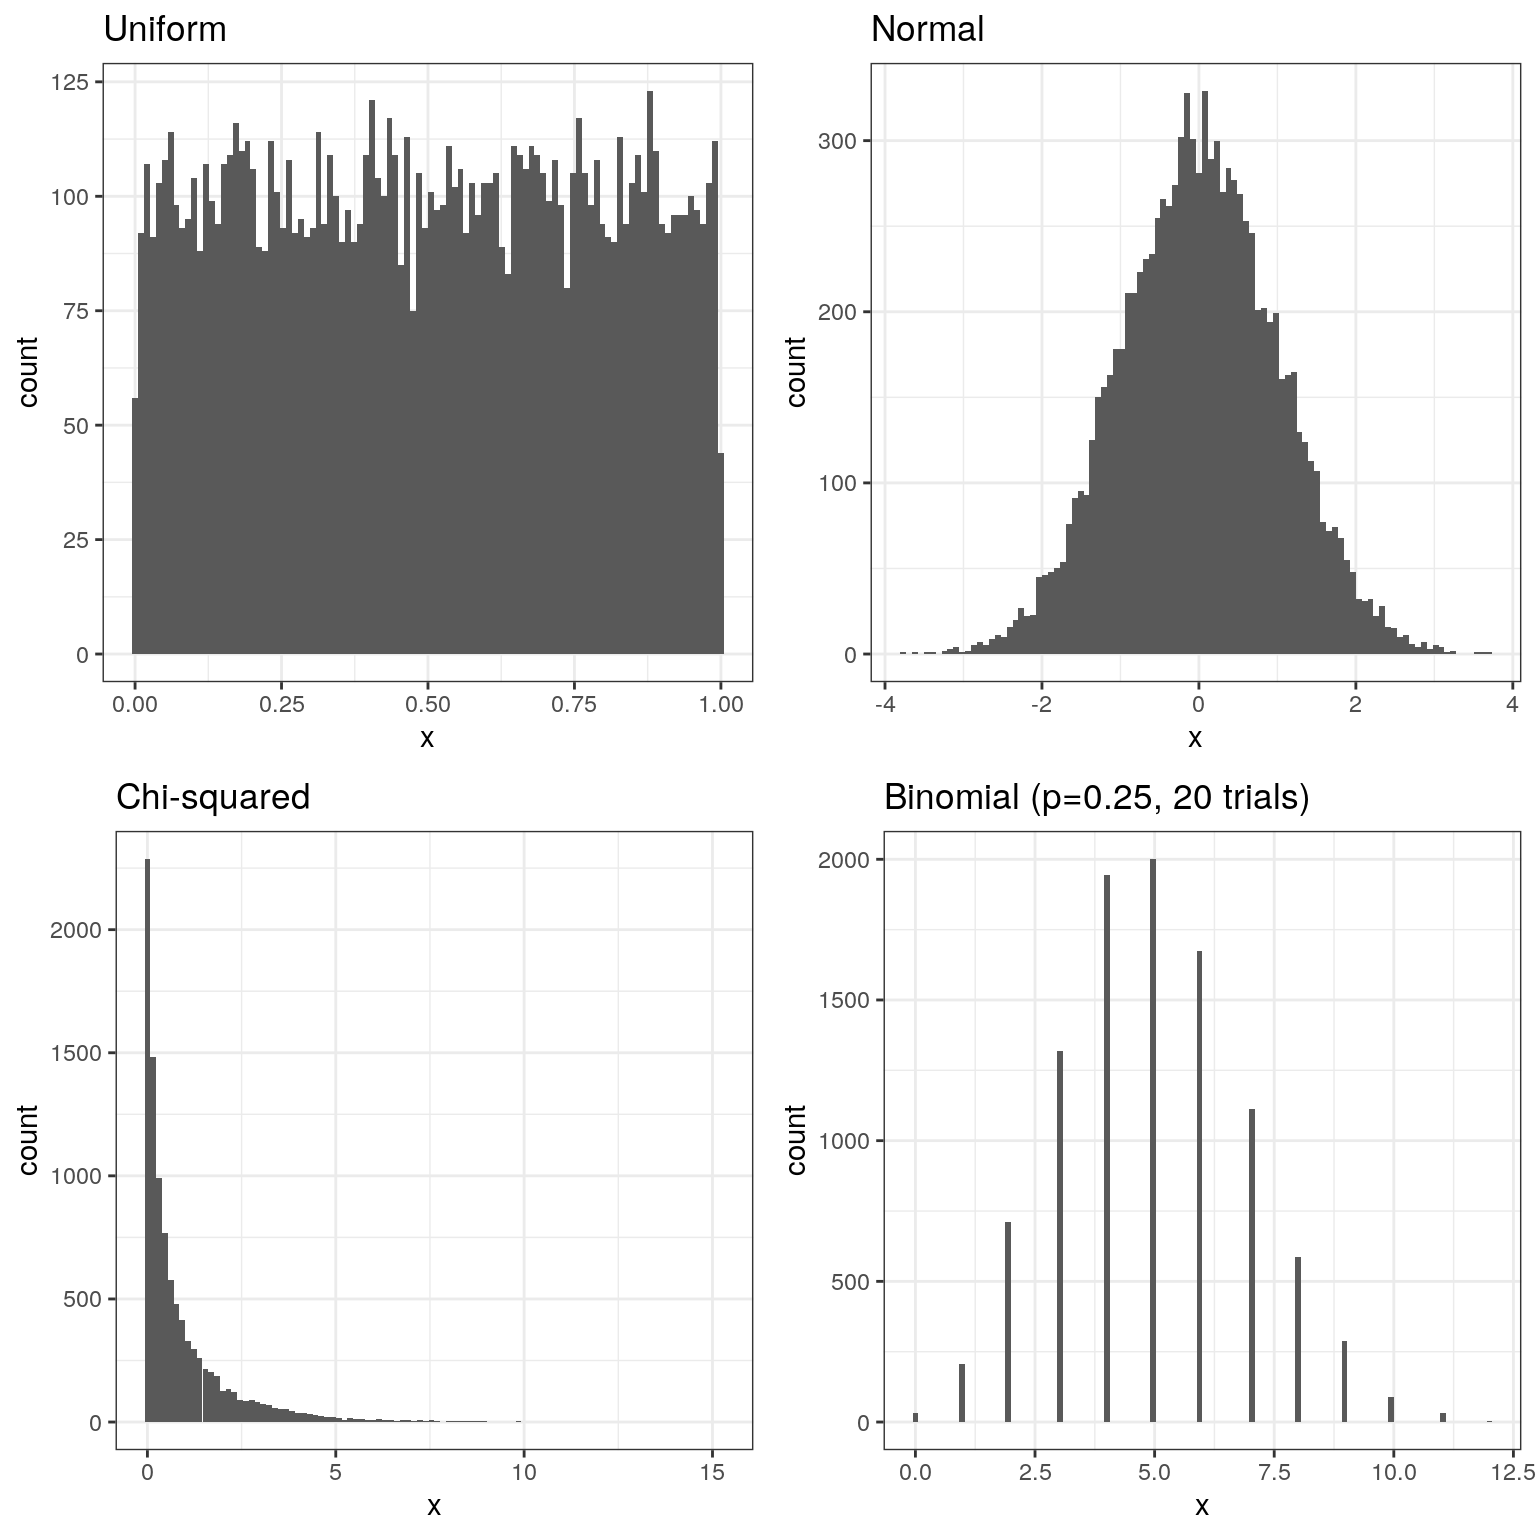
\includegraphics{StatsThinking21_files/figure-latex/unnamed-chunk-113-1.pdf}

\hypertarget{simulating-the-maximum-finishing-time}{%
\section{Simulating the maximum finishing time}\label{simulating-the-maximum-finishing-time}}

Let's simulate 150 samples, collecting the maximum value from each sample, and then plotting the distribution of maxima.

\begin{Shaded}
\begin{Highlighting}[]
\CommentTok{# sample maximum value 5000 times and compute 99th percentile}
\NormalTok{nRuns <-}\StringTok{ }\DecValTok{5000}
\NormalTok{sampSize <-}\StringTok{ }\DecValTok{150}

\NormalTok{sampleMax <-}\StringTok{ }\ControlFlowTok{function}\NormalTok{(}\DataTypeTok{sampSize =} \DecValTok{150}\NormalTok{) \{}
\NormalTok{  samp <-}\StringTok{ }\KeywordTok{rnorm}\NormalTok{(sampSize, }\DataTypeTok{mean =} \DecValTok{5}\NormalTok{, }\DataTypeTok{sd =} \DecValTok{1}\NormalTok{)}
  \KeywordTok{return}\NormalTok{(}\KeywordTok{tibble}\NormalTok{(}\DataTypeTok{max=}\KeywordTok{max}\NormalTok{(samp)))}
\NormalTok{\}}

\NormalTok{input_df <-}\StringTok{ }\KeywordTok{tibble}\NormalTok{(}\DataTypeTok{id=}\KeywordTok{seq}\NormalTok{(nRuns)) }\OperatorTok
\StringTok{  }\KeywordTok{group_by}\NormalTok{(id)}

\NormalTok{maxTime <-}\StringTok{ }\NormalTok{input_df }\OperatorTok\StringTok{ }\KeywordTok{do}\NormalTok{(}\KeywordTok{sampleMax}\NormalTok{())}

\NormalTok{cutoff <-}\StringTok{ }\KeywordTok{quantile}\NormalTok{(maxTime}\OperatorTok{$}\NormalTok{max, }\FloatTok{0.99}\NormalTok{)}


\KeywordTok{ggplot}\NormalTok{(maxTime,}\KeywordTok{aes}\NormalTok{(max)) }\OperatorTok{+}
\StringTok{  }\KeywordTok{geom_histogram}\NormalTok{(}\DataTypeTok{bins =} \DecValTok{100}\NormalTok{) }\OperatorTok{+}
\StringTok{  }\KeywordTok{geom_vline}\NormalTok{(}\DataTypeTok{xintercept =}\NormalTok{ cutoff, }\DataTypeTok{color =} \StringTok{"red"}\NormalTok{)}
\end{Highlighting}
\end{Shaded}

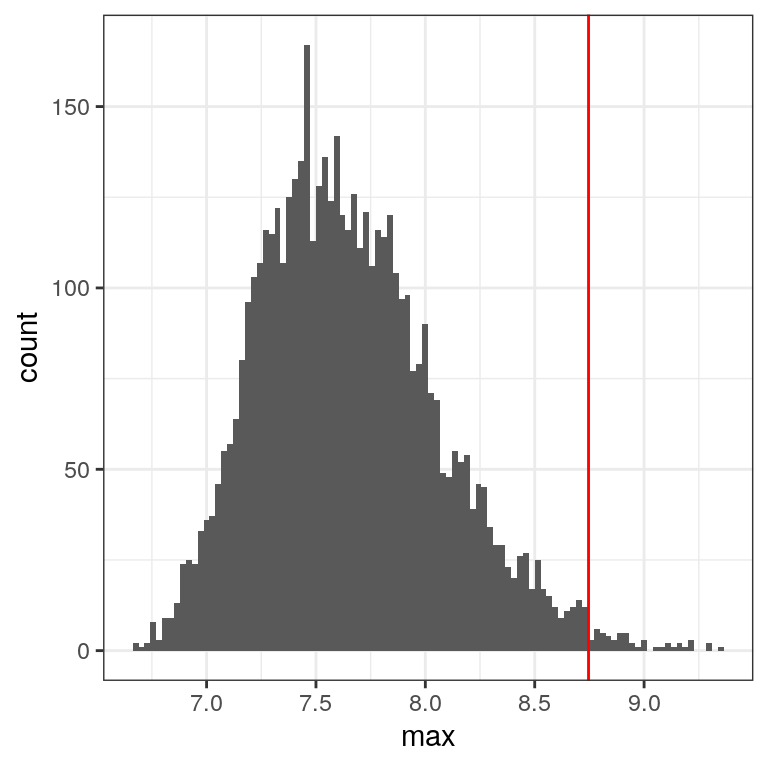
\includegraphics[width=0.5\linewidth]{StatsThinking21_files/figure-latex/unnamed-chunk-114-1}

\hypertarget{the-bootstrap}{%
\section{The bootstrap}\label{the-bootstrap}}

The bootstrap is useful for creating confidence intervals in cases where we don't have a parametric distribution. One example is for the median; let's look at how that works. We will start by implementing it by hand, to see more closely how it works. We will start by collecting a sample of individuals from the NHANES dataset, and the using the bootstrap to obtain confidence intervals on the median for the Height variable.

\begin{tabular}{r|r|r}
\hline
Lower CI limit & Median & Upper CI limit\\
\hline
161.6 & 167.65 & 171.1\\
\hline
\end{tabular}

\hypertarget{hypothesis-testing-in-r}{%
\chapter{Hypothesis testing in R}\label{hypothesis-testing-in-r}}

In this chapter we will present several examples of using R to perform hypothesis testing.

\hypertarget{simple-example-coin-flipping-section-refrandomization-very-simple}{%
\section{Simple example: Coin-flipping (Section \ref{randomization-very-simple})}\label{simple-example-coin-flipping-section-refrandomization-very-simple}}

Let's say that we flipped 100 coins and observed 70 heads. We would like to use these data to test the hypothesis that the true probability is 0.5.

First let's generate our data, simulating 100,000 sets of 100 flips. We use such a large number because it turns out that it's very rare to get 70 heads, so we need many attempts in order to get a reliable estimate of these probabilties. This will take a couple of minutes to complete.

\begin{Shaded}
\begin{Highlighting}[]
\CommentTok{# simulate tossing of 100,000 flips of 100 coins to identify }
\CommentTok{# empirical probability of 70 or more heads out of 100 flips}

\NormalTok{nRuns <-}\StringTok{ }\DecValTok{100000}

\CommentTok{# create function to toss coins}
\NormalTok{tossCoins <-}\StringTok{ }\ControlFlowTok{function}\NormalTok{() \{}
\NormalTok{  flips <-}\StringTok{ }\KeywordTok{runif}\NormalTok{(}\DecValTok{100}\NormalTok{) }\OperatorTok{>}\StringTok{ }\FloatTok{0.5} 
  \KeywordTok{return}\NormalTok{(}\KeywordTok{tibble}\NormalTok{(}\DataTypeTok{nHeads=}\KeywordTok{sum}\NormalTok{(flips)))}
\NormalTok{\}}

\CommentTok{# create an input data frame for do()}
\NormalTok{input_df <-}\StringTok{ }\KeywordTok{tibble}\NormalTok{(}\DataTypeTok{id=}\KeywordTok{seq}\NormalTok{(nRuns)) }\OperatorTok
\StringTok{  }\KeywordTok{group_by}\NormalTok{(id)}

\CommentTok{# use do() to perform the coin flips}
\NormalTok{flip_results <-}\StringTok{ }\NormalTok{input_df }\OperatorTok
\StringTok{  }\KeywordTok{do}\NormalTok{(}\KeywordTok{tossCoins}\NormalTok{()) }\OperatorTok
\StringTok{  }\KeywordTok{ungroup}\NormalTok{()}

\NormalTok{p_ge_}\DecValTok{70}\NormalTok{_sim <-}\StringTok{ }
\StringTok{  }\NormalTok{flip_results }\OperatorTok
\StringTok{  }\KeywordTok{summarise}\NormalTok{(}\DataTypeTok{p_gt_70 =} \KeywordTok{mean}\NormalTok{(nHeads }\OperatorTok{>=}\StringTok{ }\DecValTok{70}\NormalTok{)) }\OperatorTok
\StringTok{  }\KeywordTok{pull}\NormalTok{()}

\NormalTok{p_ge_}\DecValTok{70}\NormalTok{_sim}
\end{Highlighting}
\end{Shaded}

\begin{verbatim}
## [1] 3e-05
\end{verbatim}

For comparison, we can also compute the p-value for 70 or more heads based on a null hypothesis of \(P_{heads}=0.5\), using the binomial distribution.

\begin{Shaded}
\begin{Highlighting}[]
\CommentTok{# compute the probability of 69 or fewer heads, }
\CommentTok{# when P(heads)=0.5}
\NormalTok{p_lt_}\DecValTok{70}\NormalTok{ <-}\StringTok{ }\KeywordTok{pbinom}\NormalTok{(}\DecValTok{69}\NormalTok{, }\DecValTok{100}\NormalTok{, }\FloatTok{0.5}\NormalTok{) }

\CommentTok{# the probability of 70 or more heads is simply }
\CommentTok{# the complement of p_lt_70}
\NormalTok{p_ge_}\DecValTok{70}\NormalTok{ <-}\StringTok{ }\DecValTok{1} \OperatorTok{-}\StringTok{ }\NormalTok{p_lt_}\DecValTok{70}

\NormalTok{p_ge_}\DecValTok{70}
\end{Highlighting}
\end{Shaded}

\begin{verbatim}
## [1] 3.92507e-05
\end{verbatim}

\hypertarget{simulating-p-values}{%
\section{Simulating p-values}\label{simulating-p-values}}

In this exercise we will perform hypothesis testing many times in order to test whether the p-values provided by our statistical test are valid. We will sample data from a normal distribution with a mean of zero, and for each sample perform a t-test to determine whether the mean is different from zero. We will then count how often we reject the null hypothesis; since we know that the true mean is zero, these are by definition Type I errors.

\begin{Shaded}
\begin{Highlighting}[]
\NormalTok{nRuns <-}\StringTok{ }\DecValTok{5000}

\CommentTok{# create input data frame for do()}
\NormalTok{input_df <-}\StringTok{ }\KeywordTok{tibble}\NormalTok{(}\DataTypeTok{id=}\KeywordTok{seq}\NormalTok{(nRuns)) }\OperatorTok
\StringTok{  }\KeywordTok{group_by}\NormalTok{(id)}

\CommentTok{# create a function that will take a sample}
\CommentTok{# and perform a one-sample t-test}

\NormalTok{sample_ttest <-}\StringTok{ }\ControlFlowTok{function}\NormalTok{(}\DataTypeTok{sampSize=}\DecValTok{32}\NormalTok{)\{}
\NormalTok{  tt.result <-}\StringTok{ }\KeywordTok{t.test}\NormalTok{(}\KeywordTok{rnorm}\NormalTok{(sampSize))}
  \KeywordTok{return}\NormalTok{(}\KeywordTok{tibble}\NormalTok{(}\DataTypeTok{pvalue=}\NormalTok{tt.result}\OperatorTok{$}\NormalTok{p.value))}
\NormalTok{\}}

\CommentTok{# perform simulations}

\NormalTok{sample_ttest_result <-}\StringTok{ }\NormalTok{input_df }\OperatorTok
\StringTok{  }\KeywordTok{do}\NormalTok{(}\KeywordTok{sample_ttest}\NormalTok{())}

\NormalTok{p_error <-}
\StringTok{  }\NormalTok{sample_ttest_result }\OperatorTok
\StringTok{  }\KeywordTok{ungroup}\NormalTok{() }\OperatorTok
\StringTok{  }\KeywordTok{summarize}\NormalTok{(}\DataTypeTok{p_error =} \KeywordTok{mean}\NormalTok{(pvalue}\OperatorTok{<}\NormalTok{.}\DecValTok{05}\NormalTok{)) }\OperatorTok
\StringTok{  }\KeywordTok{pull}\NormalTok{()}

\NormalTok{p_error}
\end{Highlighting}
\end{Shaded}

\begin{verbatim}
## [1] 0.0478
\end{verbatim}

We should see that the proportion of samples with \(p < .05\) is about 5\%.

\hypertarget{ci-effect-size-power}{%
\chapter{Quantifying effects and designing studies}\label{ci-effect-size-power}}

In the previous chapter we discussed how we can use data to test hypotheses. Those methods provided a binary answer: we either reject or fail to reject the null hypothesis. However, this kind of decision overlooks a couple of important questions. First, we would like to know how much uncertainty we have about the answer (regardless of which way it goes). In addition, sometimes we don't have a clear null hypothesis, so we would like to see what range of estimates are consistent with the data. Second, we would like to know how large the effect actually is, since as we saw in the weight loss example in the previous chapter, a statistically significant effect is not necessarily a practically important effect.

In this chapter we will discuss methods to address these two questions: confidence intervals to provide a measure of our uncertainty about our estimates, and effect sizes to provide a standardized way to understand how large the effects are. We will also discuss the concept of \emph{statistical power} which tells us how well we can expect to find any true effects that might exist.

\hypertarget{confidence-intervals}{%
\section{Confidence intervals}\label{confidence-intervals}}

So far in the book we have focused on estimating the specific value of a statistic. For example, let's say we want to estimate the mean weight of adults in the NHANES dataset. Let's take a sample from the dataset and estimate the mean. In this sample, the mean weight was 79.9216 kilograms. We refer to this as a \emph{point estimate} since it provides us with a single number to describe our estimate of the population parameter. However, we know from our earlier discussion of sampling error that there is some uncertainty about this estimate, which is described by the standard error. You should also remember that the standard error is determined by two components: the population standard deviation (which is the numerator), and the square root of the sample size (which is in the denominator). The population standard deviation is an unknown but fixed parameter that is not under our control, whereas the sample size \emph{is} under our control. Thus, we can decrease our uncertainty about the estimate by increasing our sample size -- up to the limit of the entire population size, at which point there is no uncertainty at all because we can just calculate the population parameter directly from the data of the entire population.

You may also remember that earlier we introduced the concept of a \emph{confidence interval}, which is a way of describing our uncertainty about a statistical estimate. Remember that a confidence interval describes an interval that will on average contain the true population parameter with a given probability; for example, the 95\% confidence interval is an interval that will capture the true population parameter 95\% of the time. Note again that this is not a statement about the population parameter; any particular confidence interval either does or does not contain the true parameter. As Jerzy Neyman, the inventor of the confidence interval, said:

\begin{quote}
``The parameter is an unknown constant and no probability statement concerning its value may be made.''(Neyman \protect\hyperlink{ref-Neyman37}{1937})
\end{quote}

The confidence interval for the mean is computed as:

\[
CI = \text{point estimate} \pm \text{critical value} * \text{standard error}
\]

where the critical value is determined by the sampling distribution of the estimate. The important question, then, is what that sampling distribution is.

\hypertarget{confidence-intervals-using-the-normal-distribution}{%
\subsection{Confidence intervals using the normal distribution}\label{confidence-intervals-using-the-normal-distribution}}

If we know the population standard deviation, then we can use the normal distribution to compute a confidence interval. We usually don't, but for our example of the NHANES dataset we do (it's 21.3040605 for weight).

Let's say that we want to compute a 95\% confidence interval for the mean. The critical value would then be the values of the standard normal distribution that capture 95\% of the distribution; these are simply the 2.5th percentile and the 97.5th percentile of the distribution, which we can compute using the \texttt{qnorm()} function in R, and come out to \(\pm 1.96\). Thus, the confidence interval for the mean (\(\bar{X}\)) is:

\[
CI = \bar{X} \pm 1.96*SE
\]

Using the estimated mean from our sample (79.9216) and the known population standard deviation, we can compute the confidence interval of {[}77.2807698,82.5624302{]}.

\hypertarget{confidence-intervals-using-the-t-distribution}{%
\subsection{Confidence intervals using the t distribution}\label{confidence-intervals-using-the-t-distribution}}

As stated above, if we knew the population standard deviation, then we could use the normal distribution to compute our confidence intervals. However, in general we don't -- in which case the \emph{t} distribution is more appropriate as a sampling distribution. Remember that the t distribution is slightly broader than the normal distribution, especially for smaller samples, which means that the confidence intervals will be slightly wider than they would if we were using the normal distribution. This incorporates the extra uncertainty that arises when we make conclusions based on small samples.

We can compute the 95\% confidence interval in a way similar to the normal distribution example above, but the critical value is determined by the 2.5th percentile and the 97.5th percentile of the \emph{t} distribution, which we can compute using the \texttt{qt()} function in R. Thus, the confidence interval for the mean (\(\bar{X}\)) is:

\[
CI = \bar{X} \pm t_{crit}*SE
\]

where \(t_{crit}\) is the critical t value.
For the NHANES weight example (with sample size of 250), the confidence interval would be 79.92 +/- 1.97 * 1.41 {[}77.15 - 82.69{]}.

Remember that this doesn't tell us anything about the probability of the true population value falling within this interval, since it is a fixed parameter (which we know is 81.7652755 because we have the entire population in this case) and it either does or does not fall within this specific interval (in this case, it does). Instead, it tells us that in the long run, if we compute the confidence interval using this procedure, 95\% of the time that confidence interval will capture the true population parameter.

\hypertarget{confidence-intervals-and-sample-size}{%
\subsection{Confidence intervals and sample size}\label{confidence-intervals-and-sample-size}}

Because the standard error decreases with sample size, the means confidence interval should get narrower as the sample size increases, providing progressively tighter bounds on our estimate. Figure \ref{fig:CISampSize} shows an example of how the confidence interval would change as a function of sample size for the weight example. From the figure it's evident that the confidence interval becomes increasingly tighter as the sample size increases, but increasing samples provide diminishing returns, consistent with the fact that the denominator of the confidence interval term is proportional to the square root of the sample size.

\begin{figure}
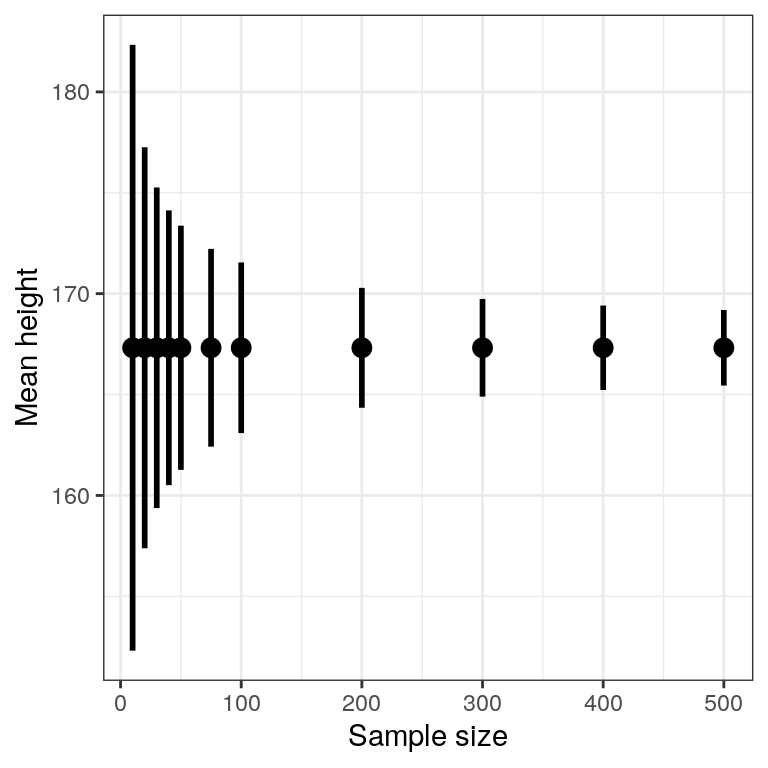
\includegraphics[height=0.5\textheight]{StatsThinking21_files/figure-latex/CISampSize-1} \caption{An example of the effect of sample size on the width of the confidence interval for the mean.}\label{fig:CISampSize}
\end{figure}

\hypertarget{computing-confidence-intervals-using-the-bootstrap}{%
\subsection{Computing confidence intervals using the bootstrap}\label{computing-confidence-intervals-using-the-bootstrap}}

In some cases we can't assume normality, or we don't know the sampling distribution of the statistic. In these cases, we can use the bootstrap (which we introduced in Chapter \ref{resampling-and-simulation}). As a reminder, the bootstrap involves repeatedly resampling the data \emph{with replacement}, and then using the distribution of the statistic computed on those samples as a surrogate for the sampling distribution of the statistic.
R includes a package called \texttt{boot} that we can use to run the bootstrap and compute confidence intervals. It's always good to use a built-in function to compute a statistic if it is available, rather than coding it up from scratch --- both because it saves you extra work, and because the built-in version will be better tested. These are the results when we use the \texttt{boot()} to compute the confidence interval for weight in our NHANES sample:

\begin{verbatim}
## BOOTSTRAP CONFIDENCE INTERVAL CALCULATIONS
## Based on 1000 bootstrap replicates
## 
## CALL : 
## boot.ci(boot.out = bs, type = "perc")
## 
## Intervals : 
## Level     Percentile     
## 95%   (77.31, 82.60 )  
## Calculations and Intervals on Original Scale
\end{verbatim}

These values are fairly close to the values obtained using the t distribution above, though not exactly the same.

\hypertarget{relation-of-confidence-intervals-to-hypothesis-tests}{%
\subsection{Relation of confidence intervals to hypothesis tests}\label{relation-of-confidence-intervals-to-hypothesis-tests}}

There is a close relationship between confidence intervals and hypothesis tests. In particular, if the confidence interval does not include the null hypothesis, then the associated statistical test would be statistically significant. For example, if you are testing whether the mean of a sample is greater than zero with \(\alpha = 0.05\), you could simply check to see whether zero is contained within the 95\% confidence interval for the mean.

Things get trickier if we want to compare the means of two conditions (Schenker and Gentleman \protect\hyperlink{ref-sche:gent:2001}{2001}). There are a couple of situations that are clear. First, if each mean is contained within the confidence interval for the other mean, then there is certainly no significant difference at the chosen confidence level. Second, if there is no overlap between the confidence intervals, then there is certainly a significant difference at the chosen level; in fact, this test is substantially \emph{conservative}, such that the actual error rate will be lower than the chosen level. But what about the case where the confidence intervals overlap one another but don't contain the means for the other group? In this case the answer depends on the relative variability of the two variables, and there is no general answer. In general we should avoid using the ``visual test'' for overlapping confidence intervals.

\hypertarget{effect-sizes}{%
\section{Effect sizes}\label{effect-sizes}}

\begin{quote}
``Statistical significance is the least interesting thing about the results. You should describe the results in terms of measures of magnitude -- not just, does a treatment affect people, but how much does it affect them.'' Gene Glass (REF)
\end{quote}

In the last chapter, we discussed the idea that statistical significance may not necessarily reflect practical significance. In order to discuss practical significance, we need a standard way to describe the size of an effect in terms of the actual data, which we refer to as an \emph{effect size}. In this section we will introduce the concept and discuss various ways that effect sizes can be calculated.

An effect size is a standardized measurement that compares the size of some statistical effect to a reference quantity, such as the variability of the statistic. In some fields of science and engineering, this idea is referred to as a ``signal to noise ratio''. There are many different ways that the effect size can be quantified, which depend on the nature of the data.

\hypertarget{cohens-d}{%
\subsection{Cohen's D}\label{cohens-d}}

One of the most common measures of effect size is known as \emph{Cohen's d}, named after the statistician Jacob Cohen (who is most famous for his 1994 paper titled ``The Earth Is Round (p \textless{} .05)''). It is used to quantify the difference between two means, in terms of their standard deviation:

\[
d = \frac{\bar{X}_1 - \bar{X}_2}{s}
\]

where \(\bar{X}_1\) and \(\bar{X}_2\) are the means of the two groups, and \(s\) is the pooled standard deviation (which is a combination of the standard deviations for the two samples, weighted by their sample sizes):

\[
s = \sqrt{\frac{(n_1 - 1)s^2_1 + (n_2 - 1)s^2_2 }{n_1 +n_2 -2}}
\]
where \(n_1\) and \(n_2\) are the sample sizes and \(s^2_1\) and \(s^2_2\) are the standard deviations for the two groups respectively. Note that this is very similar in spirit to the t statistic --- the main difference is that the denominator in the t statistic is based on the standard error of the mean, whereas the denominator in Cohen's D is based on the standard deviation of the data. This means that while the t statistic will grow as the sample size gets larger, the value of Cohen's D will remain the same.

There is a commonly used scale for interpreting the size of an effect in terms of Cohen's d:

\begin{table}

\caption{\label{tab:unnamed-chunk-125}Interpetation of Cohen's D}
\centering
\begin{tabular}[t]{l|l}
\hline
D & Interpretation\\
\hline
0.0 - 0.2 & neglibible\\
\hline
0.2 - 0.5 & small\\
\hline
0.5 - 0.8 & medium\\
\hline
0.8 - & large\\
\hline
\end{tabular}
\end{table}

It can be useful to look at some commonly understood effects to help understand these interpretations. For example, the effect size for gender differences in height (d = 1.6022439) is very large by reference to our table above. We can also see this by looking at the distributions of male and female heights in our sample. Figure \ref{fig:genderHist} shows that the two distributions are quite well separated, though still overlapping, highlighting the fact that even when there is a very large effect size for the difference between two groups, there will be individuals from each group that are more like the other group.

\begin{figure}
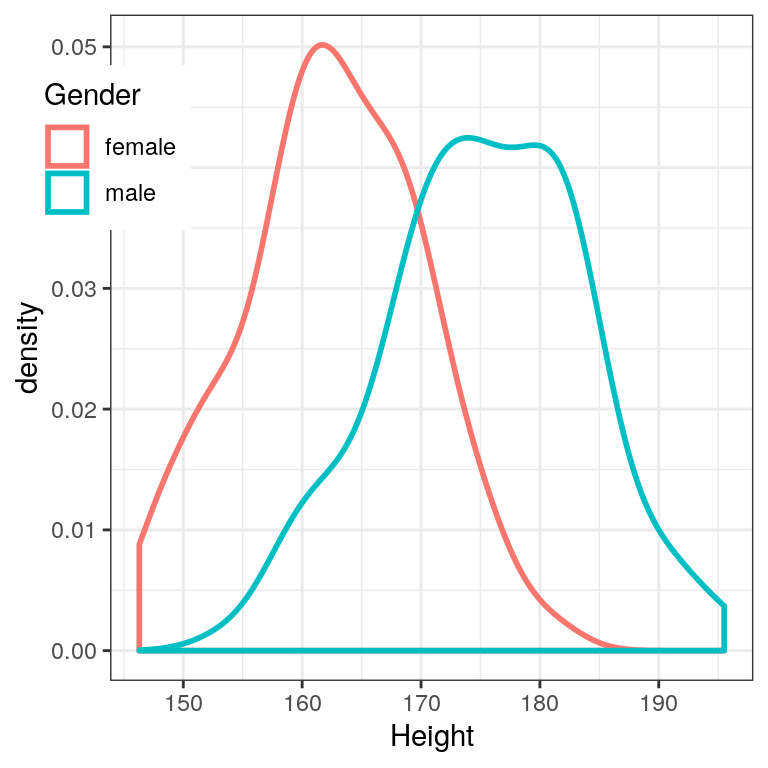
\includegraphics[height=0.5\textheight]{StatsThinking21_files/figure-latex/genderHist-1} \caption{Smoothed histogram plots for male and female heights in the NHANES dataset, showing clearly distinct but also clearly overlapping distributions.}\label{fig:genderHist}
\end{figure}

It is also worth noting that we rarely encounter effects of this magnitude in science, in part because they are such obvious effects that we don't need scientific research to find them. As we will see in Chapter \ref{doing-reproducible-research} on reproducibility, very large reported effects in scientific research often reflect the use of questionable research practices rather than truly huge effects in nature. It is also worth noting that even for such a huge effect, the two distributions still overlap - there will be some females who are taller than the average male, and vice versa. For most interesting scientific effects, the degree of overlap will be much greater, so we shouldn't immediately jump to strong conclusions about different populations based on even a large effect size.

\hypertarget{pearsons-r}{%
\subsection{Pearson's r}\label{pearsons-r}}

Pearson's \emph{r}, also known as the \emph{correlation coefficient}, is a measure of the strength of the linear relationship between two continuous variables. We will discuss correlation in much more detail in Chapter \ref{modeling-continuous-relationships}, so we will save the details for that chapter; here, we simply introduce \emph{r} as a way to quantify the relation between two variables.

\emph{r} is a measure that varies from -1 to 1, where a value of 1 represents a perfect positive relationship between the variables, 0 represents no relationship, and -1 represents a perfect negative relationship. Figure \ref{fig:corrFig} shows examples of various levels of correlation using randomly generated data.

\begin{figure}
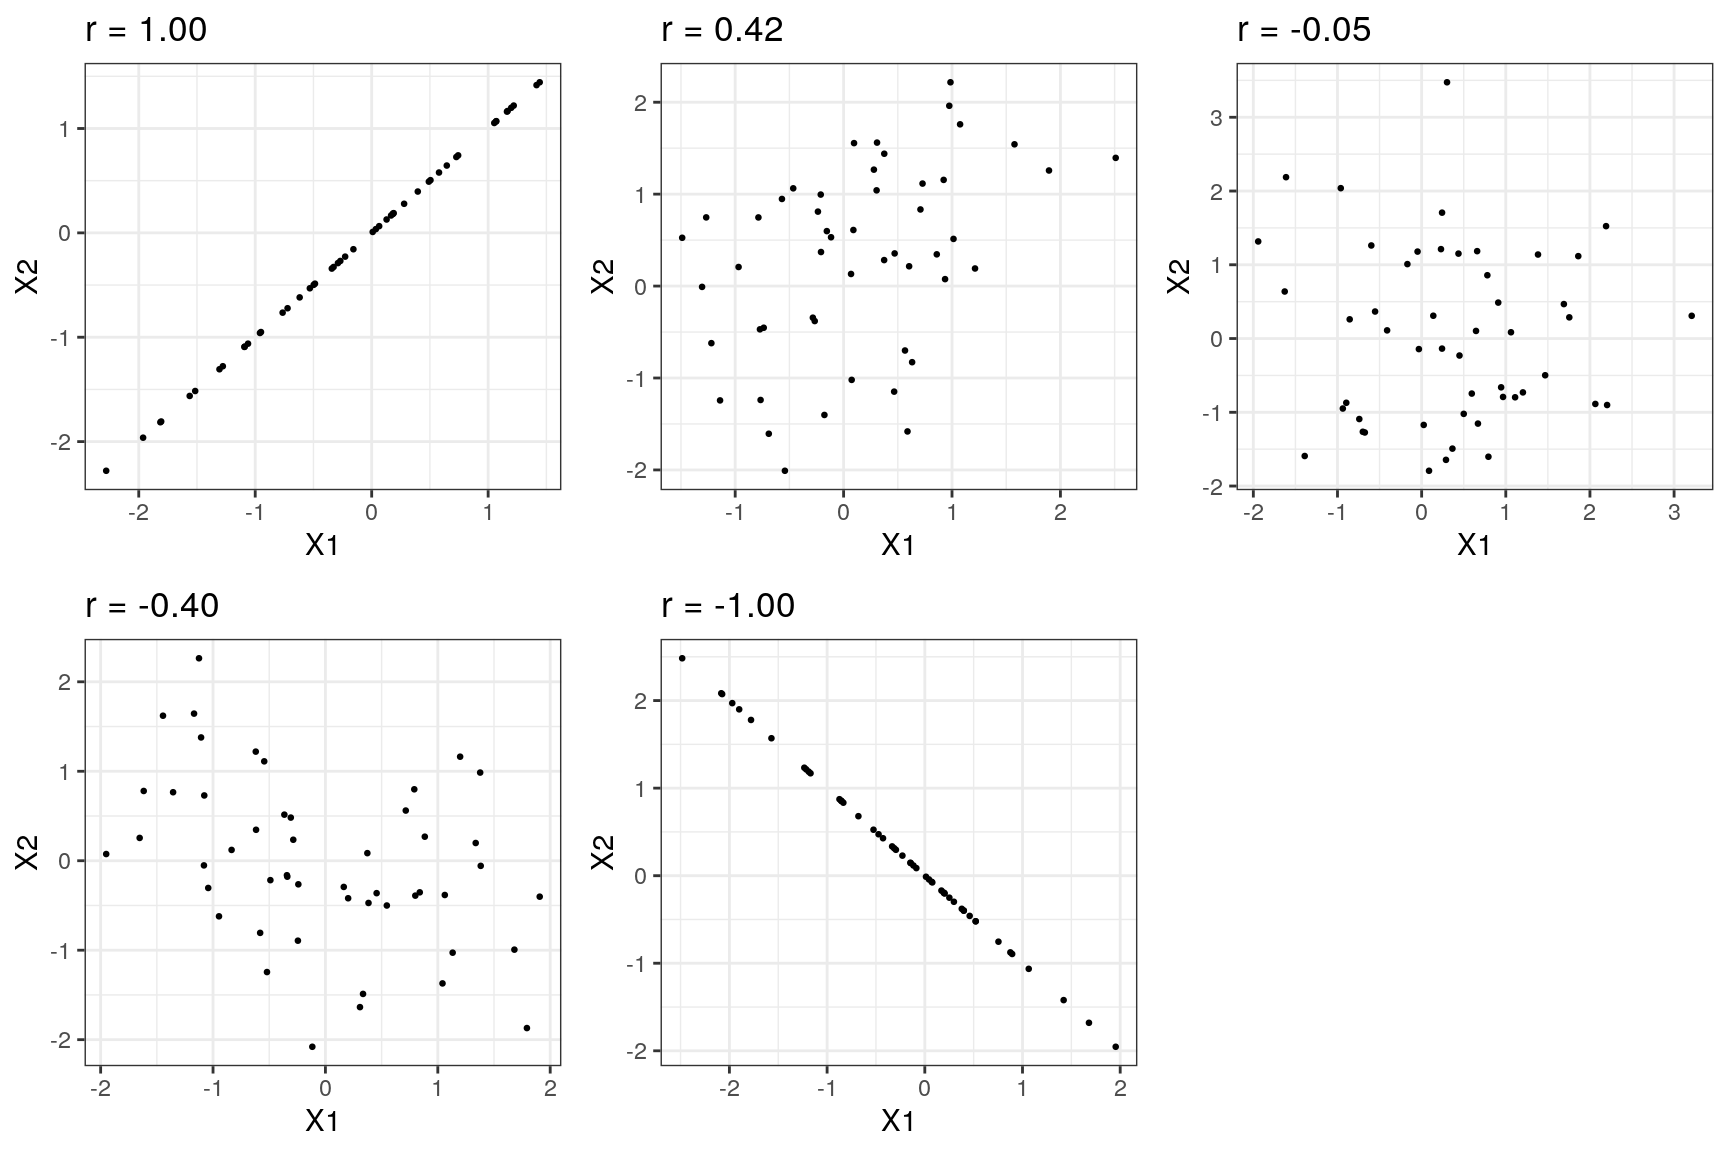
\includegraphics[height=0.5\textheight]{StatsThinking21_files/figure-latex/corrFig-1} \caption{Examples of various levels of Pearson's r.}\label{fig:corrFig}
\end{figure}

\hypertarget{odds-ratio}{%
\subsection{Odds ratio}\label{odds-ratio}}

In our earlier discussion of probability we discussed the concept of odds -- that is, the relative likelihood of some event happening versus not happening:

\[
odds\ of\ A = \frac{P(A)}{P(\neg A)}
\]

We also discussed the \emph{odds ratio}, which is simply the ratio of two odds. The odds ratio is a useful way to describe effect sizes for binary variables.

For example, let's take the case of smoking and lung cancer. A study published in the International Journal of Cancer in 2012 (Pesch et al. \protect\hyperlink{ref-pesc:kend:gust:2012}{2012}) combined data regarding the occurrence of lung cancer in smokers and individuals who have never smoked across a number of different studies. Note that these data come from case-control studies, which means that participants in the studies were recruited because they either did or did not have cancer; their smoking status was then examined. These numbers thus do not represent the prevalence of cancer amongst smokers in the general population -- but they can tell us about the relationship between cancer and smoking.

\begin{table}

\caption{\label{tab:unnamed-chunk-127}Cancer occurrence separately for current smokers and those who have never smoked}
\centering
\begin{tabular}[t]{l|r|r}
\hline
Status & NeverSmoked & CurrentSmoker\\
\hline
No Cancer & 2883 & 3829\\
\hline
Cancer & 220 & 6784\\
\hline
\end{tabular}
\end{table}

We can convert these numbers to odds ratios for each of the groups. The odds of someone having lung cancer who has never smoked is 0.0763094 whereas the odds of a current smoker having lung cancer is 1.771742. The ratio of these odds tells us about the relative likelihood of cancer between the two groups: The odds ratio of 23.2178732 tells us that the odds of cancer in smokers are roughly 23 times higher than never-smokers.

\hypertarget{statistical-power}{%
\section{Statistical power}\label{statistical-power}}

Remember from the previous chapter that under the Neyman-Pearson hypothesis testing approach, we have to specify our level of tolerance for two kinds of errors: False positives (which they called \emph{Type I error}) and false negatives (which they called \emph{Type II error}). People often focus heavily on Type I error, because making a false positive claim is generally viewed as a very bad thing; for example, the now discredited claims by Wakefield (\protect\hyperlink{ref-wake:1999}{1999}) that autism was associated with vaccination led to anti-vaccine sentiment that has resulted in substantial increases in childhood diseases such as measles. Similarly, we don't want to claim that a drug cures a disease if it really doesn't. That's why the tolerance for Type I errors is generally set fairly low, usually at \(\alpha = 0.05\). But what about Type II errors?

The concept of \emph{statistical power} is the complement of Type II error -- that is, it is the likelihood of finding a positive result given that it exists:

\[ 
power = 1 - \beta
\]

Another important aspect of the Neyman-Pearson model that we didn't discuss above is the fact that in addition to specifying the acceptable levels of Type I and Type II errors, we also have to describe a specific alternative hypothesis -- that is, what is the size of the effect that we wish to detect? Otherwise, we can't interpret \(\beta\) -- the likelihood of finding a large effect is always going to be higher than finding a small effect, so \(\beta\) will be different depending on the size of effect we are trying to detect.

There are three factors that can affect power:

\begin{itemize}
\tightlist
\item
  Sample size: Larger samples provide greater statistical power
\item
  Effect size: A given design will always have greater power to find a large effect than a small effect (because finding large effects is easier)
\item
  Type I error rate: There is a relationship between Type I error and power such that (all else being equal) decreasing Type I error will also decrease power.
\end{itemize}

We can see this through simulation. First let's simulate a single experiment, in which we compare the means of two groups using a standard t-test. We will vary the size of the effect (specified in terms of Cohen's d), the Type I error rate, and the sample size, and for each of these we will examine how the proportion of significant results (i.e.~power) is affected. Figure \ref{fig:plotPowerSim} shows an example of how power changes as a function of these factors.

\begin{figure}
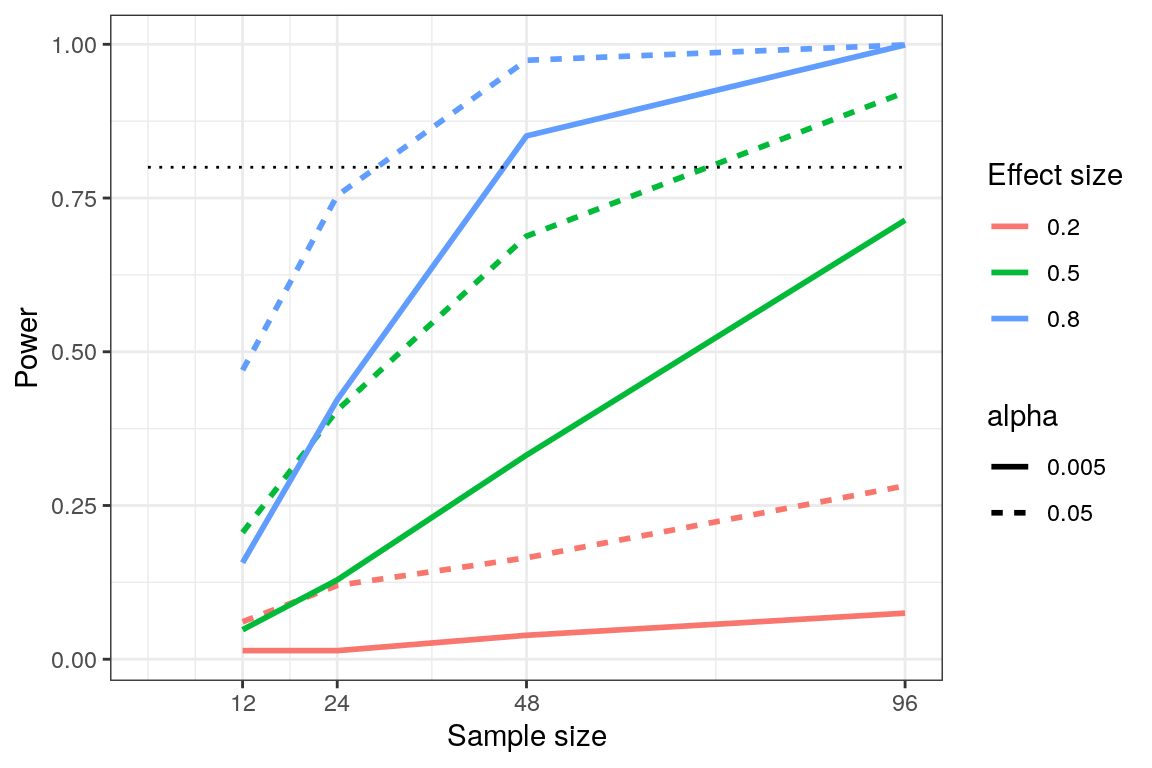
\includegraphics[height=0.5\textheight]{StatsThinking21_files/figure-latex/plotPowerSim-1} \caption{Results from power simulation, showing power as a function of sample size, with effect sizes shown as different colors, and alpha shown as line type. The standard criterion of 80 percent power is shown by the dotted black line.}\label{fig:plotPowerSim}
\end{figure}

This simulation shows us that even with a sample size of 96, we will have relatively little power to find a small effect (\(d = 0.2\)) with \(\alpha = 0.005\). This means that a study designed to do this would be \emph{futile} -- that is, it is almost guaranteed to find nothing even if a true effect of that size exists.

There are at least two important reasons to care about statistical power, one of which we discuss here and the other of which we will return to in Chapter \ref{doing-reproducible-research}. If you are a researcher, you probably don't want to spend your time doing futile experiments. Running an underpowered study is essentially futile, because it means that there is a very low likelihood that one will find an effect, even if it exists.

\hypertarget{power-analysis}{%
\subsection{Power analysis}\label{power-analysis}}

Fortunately, there are tools available that allow us to determine the statistical power of an experiment. The most common use of these tools is in planning an experiment, when we would like to determine how large our sample needs to be in order to have sufficient power to find our effect of interest.

Let's say that we are interested in running a study of how a particular personality trait differs between users of iOS versus Android devices. Our plan is collect two groups of individuals and measure them on the personality trait, and then compare the two groups using a t-test. In order to determine the necessary sample size, we can use the \texttt{power.t.test()} function:

\begin{verbatim}
## 
##      Two-sample t test power calculation 
## 
##               n = 63.76576
##           delta = 0.5
##              sd = 1
##       sig.level = 0.05
##           power = 0.8
##     alternative = two.sided
## 
## NOTE: n is number in *each* group
\end{verbatim}

This tells us that we would need at least 64 subjects in each group in order to have sufficient power to find a medium-sized effect. It's always important to run a power analysis before one starts a new study, to make sure that the study won't be futile due to a sample that is too small.

It might have occurred to you that if the effect size is large enough, then the necessary sample will be very small. For example, if we run the same power analysis with an effect size of d=2, then we will see that we only need about 5 subjects in each group to have sufficient power to find the difference.

\begin{verbatim}
## 
##      Two-sample t test power calculation 
## 
##               n = 5.089995
##               d = 2
##       sig.level = 0.05
##           power = 0.8
##     alternative = two.sided
## 
## NOTE: n is number in *each* group
\end{verbatim}

However, it's rare in science to be doing an experiment where we expect to find such a large effect -- just as we don't need statistics to tell us that 16-year-olds are taller than than 6-year-olds. When we run a power analysis, we need to specify an effect size that is plausible for our study, which would usually come from previous research. However, in Chapter \ref{doing-reproducible-research} we will discuss a phenomenon known as the ``winner's curse'' that likely results in published effect sizes being larger than the true effect size, so this should also be kept in mind.

\hypertarget{learning-objectives-1}{%
\section{Learning objectives}\label{learning-objectives-1}}

Having read this chapter, you should be able to:

\begin{itemize}
\tightlist
\item
  Describe the proper interpretation of a confidence interval, and compute a confidence interval for the mean of a given dataset.
\item
  Define the concept of effect size, and compute the effect size for a given test.
\end{itemize}

\hypertarget{suggested-readings}{%
\section{Suggested readings}\label{suggested-readings}}

\begin{itemize}
\tightlist
\item
  \href{http://www.ejwagenmakers.com/inpress/HoekstraEtAlPBR.pdf}{Robust misinterpretation of confidence intervals, by Hoekstra et al.}
\end{itemize}

\hypertarget{statistical-power-in-r}{%
\chapter{Statistical power in R}\label{statistical-power-in-r}}

In this chapter we focus specifically on statistical power.

\hypertarget{power-analysis-1}{%
\section{Power analysis}\label{power-analysis-1}}

We can compute a power analysis using functions from the \texttt{pwr} package. Let's focus on the power for a t-test in order to determine a difference in the mean between two groups. Let's say that we think than an effect size of Cohen's d=0.5 is realistic for the study in question (based on previous research) and would be of scientific interest. We wish to have 80\% power to find the effect if it exists. We can compute the sample size needed for adequate power using the \texttt{pwr.t.test()} function:

\begin{Shaded}
\begin{Highlighting}[]
\KeywordTok{pwr.t.test}\NormalTok{(}\DataTypeTok{d=}\FloatTok{0.5}\NormalTok{, }\DataTypeTok{power=}\NormalTok{.}\DecValTok{8}\NormalTok{)}
\end{Highlighting}
\end{Shaded}

\begin{verbatim}
## 
##      Two-sample t test power calculation 
## 
##               n = 63.76561
##               d = 0.5
##       sig.level = 0.05
##           power = 0.8
##     alternative = two.sided
## 
## NOTE: n is number in *each* group
\end{verbatim}

Thus, about 64 participants would be needed in each group in order to test the hypothesis with adequate power.

\hypertarget{power-curves}{%
\section{Power curves}\label{power-curves}}

We can also create plots that can show us how the power to find an effect varies as a function of effect size and sample size. We willl use the \texttt{crossing()} function from the \texttt{tidyr} package to help with this. This function takes in two vectors, and returns a tibble that contains all possible combinations of those values.

\begin{Shaded}
\begin{Highlighting}[]
\NormalTok{effect_sizes <-}\StringTok{ }\KeywordTok{c}\NormalTok{(}\FloatTok{0.2}\NormalTok{, }\FloatTok{0.5}\NormalTok{, }\FloatTok{0.8}\NormalTok{) }
\NormalTok{sample_sizes =}\StringTok{ }\KeywordTok{seq}\NormalTok{(}\DecValTok{10}\NormalTok{, }\DecValTok{500}\NormalTok{, }\DecValTok{10}\NormalTok{)}

\CommentTok{#}
\NormalTok{input_df <-}\StringTok{ }\KeywordTok{crossing}\NormalTok{(effect_sizes,sample_sizes)}
\KeywordTok{glimpse}\NormalTok{(input_df)}
\end{Highlighting}
\end{Shaded}

\begin{verbatim}
## Observations: 150
## Variables: 2
## $ effect_sizes <dbl> 0.2, 0.2, 0.2, 0.2, 0.2, 0.2, 0.2,...
## $ sample_sizes <dbl> 10, 20, 30, 40, 50, 60, 70, 80, 90...
\end{verbatim}

Using this, we can then perform a power analysis for each combination of effect size and sample size to create our power curves. In this case, let's say that we wish to perform a two-sample t-test.

\begin{Shaded}
\begin{Highlighting}[]
\CommentTok{# create a function get the power value and}
\CommentTok{# return as a tibble}
\NormalTok{get_power <-}\StringTok{ }\ControlFlowTok{function}\NormalTok{(df)\{}
\NormalTok{  power_result <-}\StringTok{ }\KeywordTok{pwr.t.test}\NormalTok{(}\DataTypeTok{n=}\NormalTok{df}\OperatorTok{$}\NormalTok{sample_sizes, }
                             \DataTypeTok{d=}\NormalTok{df}\OperatorTok{$}\NormalTok{effect_sizes,}
                             \DataTypeTok{type=}\StringTok{'two.sample'}\NormalTok{)}
\NormalTok{  df}\OperatorTok{$}\NormalTok{power=power_result}\OperatorTok{$}\NormalTok{power}
  \KeywordTok{return}\NormalTok{(df)}
\NormalTok{\}}

\CommentTok{# run get_power for each combination of effect size }
\CommentTok{# and sample size}

\NormalTok{power_curves <-}\StringTok{ }\NormalTok{input_df }\OperatorTok
\StringTok{  }\KeywordTok{do}\NormalTok{(}\KeywordTok{get_power}\NormalTok{(.)) }\OperatorTok
\StringTok{  }\KeywordTok{mutate}\NormalTok{(}\DataTypeTok{effect_sizes =} \KeywordTok{as.factor}\NormalTok{(effect_sizes)) }
\end{Highlighting}
\end{Shaded}

Now we can plot the power curves, using a separate line for each effect size.

\begin{Shaded}
\begin{Highlighting}[]
\KeywordTok{ggplot}\NormalTok{(power_curves, }
       \KeywordTok{aes}\NormalTok{(}\DataTypeTok{x=}\NormalTok{sample_sizes,}
           \DataTypeTok{y=}\NormalTok{power, }
           \DataTypeTok{linetype=}\NormalTok{effect_sizes)) }\OperatorTok{+}\StringTok{ }
\StringTok{  }\KeywordTok{geom_line}\NormalTok{() }\OperatorTok{+}\StringTok{ }
\StringTok{  }\KeywordTok{geom_hline}\NormalTok{(}\DataTypeTok{yintercept =} \FloatTok{0.8}\NormalTok{, }
             \DataTypeTok{linetype=}\StringTok{'dotdash'}\NormalTok{)}
\end{Highlighting}
\end{Shaded}

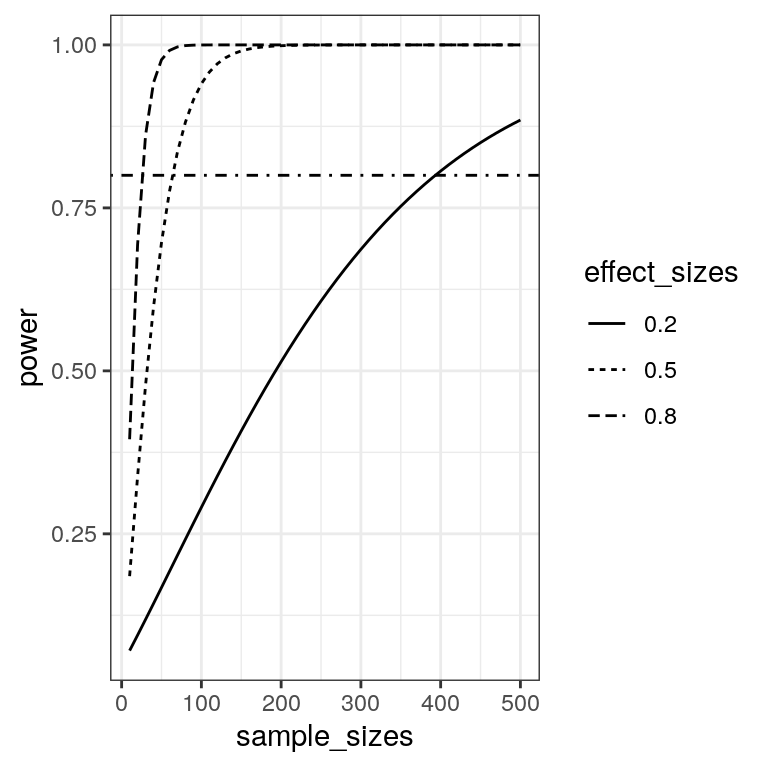
\includegraphics[width=0.5\linewidth]{StatsThinking21_files/figure-latex/unnamed-chunk-135-1}

\hypertarget{simulating-statistical-power}{%
\section{Simulating statistical power}\label{simulating-statistical-power}}

Let's simulate this to see whether the power analysis actually gives the right answer.
We will sample data for two groups, with a difference of 0.5 standard deviations between their underlying distributions, and we will look at how often we reject the null hypothesis.

\begin{Shaded}
\begin{Highlighting}[]
\NormalTok{nRuns <-}\StringTok{ }\DecValTok{5000}
\NormalTok{effectSize <-}\StringTok{ }\FloatTok{0.5}
\CommentTok{# perform power analysis to get sample size}
\NormalTok{pwr.result <-}\StringTok{ }\KeywordTok{pwr.t.test}\NormalTok{(}\DataTypeTok{d=}\NormalTok{effectSize, }\DataTypeTok{power=}\NormalTok{.}\DecValTok{8}\NormalTok{)}
\CommentTok{# round up from estimated sample size}
\NormalTok{sampleSize <-}\StringTok{ }\KeywordTok{ceiling}\NormalTok{(pwr.result}\OperatorTok{$}\NormalTok{n)}

\CommentTok{# create a function that will generate samples and test for}
\CommentTok{# a difference between groups using a two-sample t-test}

\NormalTok{get_t_result <-}\StringTok{ }\ControlFlowTok{function}\NormalTok{(sampleSize, effectSize)\{}
  \CommentTok{# take sample for the first group from N(0, 1)}
\NormalTok{  group1 <-}\StringTok{ }\KeywordTok{rnorm}\NormalTok{(sampleSize)}
\NormalTok{  group2 <-}\StringTok{ }\KeywordTok{rnorm}\NormalTok{(sampleSize, }\DataTypeTok{mean=}\NormalTok{effectSize)}
\NormalTok{  ttest.result <-}\StringTok{ }\KeywordTok{t.test}\NormalTok{(group1, group2)}
  \KeywordTok{return}\NormalTok{(}\KeywordTok{tibble}\NormalTok{(}\DataTypeTok{pvalue=}\NormalTok{ttest.result}\OperatorTok{$}\NormalTok{p.value))}
\NormalTok{\}}

\NormalTok{index_df <-}\StringTok{ }\KeywordTok{tibble}\NormalTok{(}\DataTypeTok{id=}\KeywordTok{seq}\NormalTok{(nRuns)) }\OperatorTok
\StringTok{  }\KeywordTok{group_by}\NormalTok{(id)}

\NormalTok{power_sim_results <-}\StringTok{ }\NormalTok{index_df }\OperatorTok
\StringTok{  }\KeywordTok{do}\NormalTok{(}\KeywordTok{get_t_result}\NormalTok{(sampleSize, effectSize))}

\NormalTok{p_reject <-}
\StringTok{  }\NormalTok{power_sim_results }\OperatorTok
\StringTok{  }\KeywordTok{ungroup}\NormalTok{() }\OperatorTok
\StringTok{  }\KeywordTok{summarize}\NormalTok{(}\DataTypeTok{pvalue =} \KeywordTok{mean}\NormalTok{(pvalue}\OperatorTok{<}\NormalTok{.}\DecValTok{05}\NormalTok{)) }\OperatorTok
\StringTok{  }\KeywordTok{pull}\NormalTok{()}

\NormalTok{p_reject}
\end{Highlighting}
\end{Shaded}

\begin{verbatim}
## [1] 0.7998
\end{verbatim}

This should return a number very close to 0.8.

\hypertarget{bayesian-statistics-in-r}{%
\chapter{Bayesian statistics in R}\label{bayesian-statistics-in-r}}

\hypertarget{a-simple-example-section-refdoing-bayesian-estimation}{%
\section{A simple example (Section \ref{doing-bayesian-estimation})}\label{a-simple-example-section-refdoing-bayesian-estimation}}

\begin{Shaded}
\begin{Highlighting}[]
\NormalTok{bayes_df =}\StringTok{ }\KeywordTok{data.frame}\NormalTok{(}\DataTypeTok{prior=}\OtherTok{NA}\NormalTok{, }
                      \DataTypeTok{likelihood=}\OtherTok{NA}\NormalTok{, }
                      \DataTypeTok{marginal_likelihood=}\OtherTok{NA}\NormalTok{, }
                      \DataTypeTok{posterior=}\OtherTok{NA}\NormalTok{)}

\NormalTok{bayes_df}\OperatorTok{$}\NormalTok{prior <-}\StringTok{ }\DecValTok{1}\OperatorTok{/}\DecValTok{1000000} 


\NormalTok{nTests <-}\StringTok{ }\DecValTok{3}
\NormalTok{nPositives <-}\StringTok{ }\DecValTok{3}
\NormalTok{sensitivity <-}\StringTok{ }\FloatTok{0.99}
\NormalTok{specificity <-}\StringTok{ }\FloatTok{0.99}

\NormalTok{bayes_df}\OperatorTok{$}\NormalTok{likelihood <-}\StringTok{ }\KeywordTok{dbinom}\NormalTok{(nPositives, nTests, }\FloatTok{0.99}\NormalTok{)}

\NormalTok{bayes_df}\OperatorTok{$}\NormalTok{marginal_likelihood <-}\StringTok{ }
\StringTok{  }\KeywordTok{dbinom}\NormalTok{(}
    \DataTypeTok{x =}\NormalTok{ nPositives, }
    \DataTypeTok{size =}\NormalTok{ nTests, }
    \DataTypeTok{prob =}\NormalTok{ sensitivity}
\NormalTok{  ) }\OperatorTok{*}\StringTok{ }\NormalTok{bayes_df}\OperatorTok{$}\NormalTok{prior }\OperatorTok{+}\StringTok{ }
\StringTok{  }\KeywordTok{dbinom}\NormalTok{(}
    \DataTypeTok{x =}\NormalTok{ nPositives, }
    \DataTypeTok{size =}\NormalTok{ nTests, }
    \DataTypeTok{prob =} \DecValTok{1} \OperatorTok{-}\StringTok{ }\NormalTok{specificity}
\NormalTok{  ) }\OperatorTok{*}\StringTok{ }
\StringTok{  }\NormalTok{(}\DecValTok{1} \OperatorTok{-}\StringTok{ }\NormalTok{bayes_df}\OperatorTok{$}\NormalTok{prior)}

\NormalTok{bayes_df}\OperatorTok{$}\NormalTok{posterior <-}\StringTok{ }
\StringTok{  }\NormalTok{(bayes_df}\OperatorTok{$}\NormalTok{likelihood }\OperatorTok{*}\StringTok{ }\NormalTok{bayes_df}\OperatorTok{$}\NormalTok{prior) }\OperatorTok{/}\StringTok{ }
\StringTok{  }\NormalTok{bayes_df}\OperatorTok{$}\NormalTok{marginal_likelihood}
\end{Highlighting}
\end{Shaded}

\hypertarget{estimating-posterior-distributions-section-refestimating-posterior-distributions}{%
\section{Estimating posterior distributions (Section \ref{estimating-posterior-distributions})}\label{estimating-posterior-distributions-section-refestimating-posterior-distributions}}

\begin{Shaded}
\begin{Highlighting}[]
\CommentTok{# create a table with results}
\NormalTok{nResponders <-}\StringTok{ }\DecValTok{64}
\NormalTok{nTested <-}\StringTok{ }\DecValTok{100}

\NormalTok{drugDf <-}\StringTok{ }\KeywordTok{tibble}\NormalTok{(}
  \DataTypeTok{outcome =} \KeywordTok{c}\NormalTok{(}\StringTok{"improved"}\NormalTok{, }\StringTok{"not improved"}\NormalTok{),}
  \DataTypeTok{number =} \KeywordTok{c}\NormalTok{(nResponders, nTested }\OperatorTok{-}\StringTok{ }\NormalTok{nResponders)}
\NormalTok{)}
\end{Highlighting}
\end{Shaded}

Computing likelihood

\begin{Shaded}
\begin{Highlighting}[]
\NormalTok{likeDf <-}
\StringTok{  }\KeywordTok{tibble}\NormalTok{(}\DataTypeTok{resp =} \KeywordTok{seq}\NormalTok{(}\DecValTok{1}\NormalTok{,}\DecValTok{99}\NormalTok{,}\DecValTok{1}\NormalTok{)) }\OperatorTok
\StringTok{  }\KeywordTok{mutate}\NormalTok{(}
    \DataTypeTok{presp=}\NormalTok{resp}\OperatorTok{/}\DecValTok{100}\NormalTok{,}
    \DataTypeTok{likelihood5 =} \KeywordTok{dbinom}\NormalTok{(resp,}\DecValTok{100}\NormalTok{,.}\DecValTok{5}\NormalTok{),}
    \DataTypeTok{likelihood7 =} \KeywordTok{dbinom}\NormalTok{(resp,}\DecValTok{100}\NormalTok{,.}\DecValTok{7}\NormalTok{),}
    \DataTypeTok{likelihood3 =} \KeywordTok{dbinom}\NormalTok{(resp,}\DecValTok{100}\NormalTok{,.}\DecValTok{3}\NormalTok{)}
\NormalTok{)}

\KeywordTok{ggplot}\NormalTok{(likeDf,}\KeywordTok{aes}\NormalTok{(resp,likelihood5)) }\OperatorTok{+}\StringTok{ }
\StringTok{  }\KeywordTok{geom_line}\NormalTok{() }\OperatorTok{+}
\StringTok{  }\KeywordTok{xlab}\NormalTok{(}\StringTok{'number of responders'}\NormalTok{) }\OperatorTok{+}\StringTok{ }\KeywordTok{ylab}\NormalTok{(}\StringTok{'likelihood'}\NormalTok{) }\OperatorTok{+}
\StringTok{  }\KeywordTok{geom_vline}\NormalTok{(}\DataTypeTok{xintercept =}\NormalTok{ drugDf}\OperatorTok{$}\NormalTok{number[}\DecValTok{1}\NormalTok{],}\DataTypeTok{color=}\StringTok{'blue'}\NormalTok{) }\OperatorTok{+}
\StringTok{  }\KeywordTok{geom_line}\NormalTok{(}\KeywordTok{aes}\NormalTok{(resp,likelihood7),}\DataTypeTok{linetype=}\StringTok{'dotted'}\NormalTok{) }\OperatorTok{+}
\StringTok{  }\KeywordTok{geom_line}\NormalTok{(}\KeywordTok{aes}\NormalTok{(resp,likelihood3),}\DataTypeTok{linetype=}\StringTok{'dashed'}\NormalTok{)}
\end{Highlighting}
\end{Shaded}

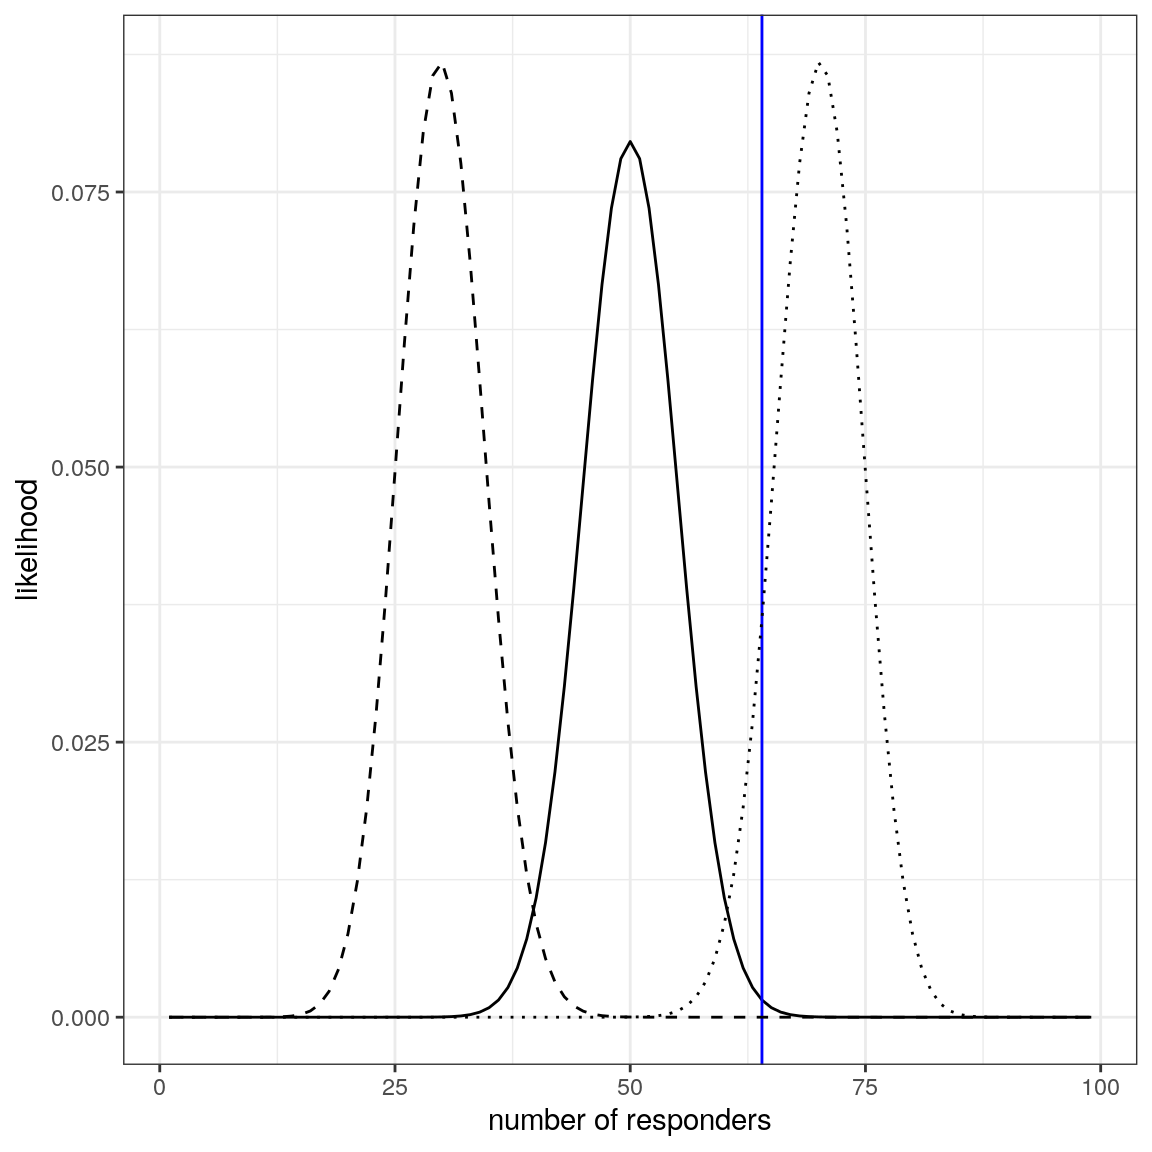
\includegraphics{StatsThinking21_files/figure-latex/unnamed-chunk-140-1.pdf}

Computing marginal likelihood

\begin{Shaded}
\begin{Highlighting}[]
\CommentTok{# compute marginal likelihood}
\NormalTok{likeDf <-}\StringTok{ }
\StringTok{  }\NormalTok{likeDf }\OperatorTok
\StringTok{  }\KeywordTok{mutate}\NormalTok{(}\DataTypeTok{uniform_prior =} \KeywordTok{array}\NormalTok{(}\DecValTok{1} \OperatorTok{/}\StringTok{ }\KeywordTok{n}\NormalTok{()))}

\CommentTok{# multiply each likelihood by prior and add them up}
\NormalTok{marginal_likelihood <-}\StringTok{ }
\StringTok{  }\KeywordTok{sum}\NormalTok{(}
    \KeywordTok{dbinom}\NormalTok{(}
      \DataTypeTok{x =}\NormalTok{ nResponders, }\CommentTok{# the number who responded to the drug}
      \DataTypeTok{size =} \DecValTok{100}\NormalTok{, }\CommentTok{# the number tested}
\NormalTok{      likeDf}\OperatorTok{$}\NormalTok{presp }\CommentTok{# the likelihood of each response }
\NormalTok{    ) }\OperatorTok{*}\StringTok{ }\NormalTok{likeDf}\OperatorTok{$}\NormalTok{uniform_prior}
\NormalTok{  )}
\end{Highlighting}
\end{Shaded}

Comuting posterior

\begin{Shaded}
\begin{Highlighting}[]
\NormalTok{bayesDf <-}
\StringTok{  }\KeywordTok{tibble}\NormalTok{(}
    \DataTypeTok{steps =} \KeywordTok{seq}\NormalTok{(}\DataTypeTok{from =} \FloatTok{0.01}\NormalTok{, }\DataTypeTok{to =} \FloatTok{0.99}\NormalTok{, }\DataTypeTok{by =} \FloatTok{0.01}\NormalTok{)}
\NormalTok{  ) }\OperatorTok
\StringTok{  }\KeywordTok{mutate}\NormalTok{(}
    \DataTypeTok{likelihoods =} \KeywordTok{dbinom}\NormalTok{(}
      \DataTypeTok{x =}\NormalTok{ nResponders, }
      \DataTypeTok{size =} \DecValTok{100}\NormalTok{, }
      \DataTypeTok{prob =}\NormalTok{ steps}
\NormalTok{    ),}
    \DataTypeTok{priors =} \KeywordTok{dunif}\NormalTok{(steps) }\OperatorTok{/}\StringTok{ }\KeywordTok{length}\NormalTok{(steps),}
    \DataTypeTok{posteriors =}\NormalTok{ (likelihoods }\OperatorTok{*}\StringTok{ }\NormalTok{priors) }\OperatorTok{/}\StringTok{ }\NormalTok{marginal_likelihood}
\NormalTok{  )}

\CommentTok{# compute MAP estimate}
\NormalTok{MAP_estimate <-}\StringTok{ }
\StringTok{  }\NormalTok{bayesDf }\OperatorTok\StringTok{ }
\StringTok{  }\KeywordTok{arrange}\NormalTok{(}\KeywordTok{desc}\NormalTok{(posteriors)) }\OperatorTok\StringTok{ }
\StringTok{  }\KeywordTok{slice}\NormalTok{(}\DecValTok{1}\NormalTok{) }\OperatorTok\StringTok{ }
\StringTok{  }\KeywordTok{pull}\NormalTok{(steps)}



\KeywordTok{ggplot}\NormalTok{(bayesDf,}\KeywordTok{aes}\NormalTok{(steps,posteriors)) }\OperatorTok{+}
\StringTok{  }\KeywordTok{geom_line}\NormalTok{() }\OperatorTok{+}
\StringTok{  }\KeywordTok{geom_line}\NormalTok{(}\KeywordTok{aes}\NormalTok{(steps,priors),}
            \DataTypeTok{color=}\StringTok{'black'}\NormalTok{,}
            \DataTypeTok{linetype=}\StringTok{'dotted'}\NormalTok{) }\OperatorTok{+}
\StringTok{  }\KeywordTok{xlab}\NormalTok{(}\StringTok{'p(respond)'}\NormalTok{) }\OperatorTok{+}\StringTok{ }
\StringTok{  }\KeywordTok{ylab}\NormalTok{(}\StringTok{'posterior probability of the observed data'}\NormalTok{) }\OperatorTok{+}
\StringTok{  }\KeywordTok{annotate}\NormalTok{(}
    \StringTok{"point"}\NormalTok{, }
    \DataTypeTok{x =}\NormalTok{ MAP_estimate, }
    \DataTypeTok{y =} \KeywordTok{max}\NormalTok{(bayesDf}\OperatorTok{$}\NormalTok{posteriors), }
    \DataTypeTok{shape=}\DecValTok{9}\NormalTok{, }
    \DataTypeTok{size =} \DecValTok{3}
\NormalTok{  )}
\end{Highlighting}
\end{Shaded}

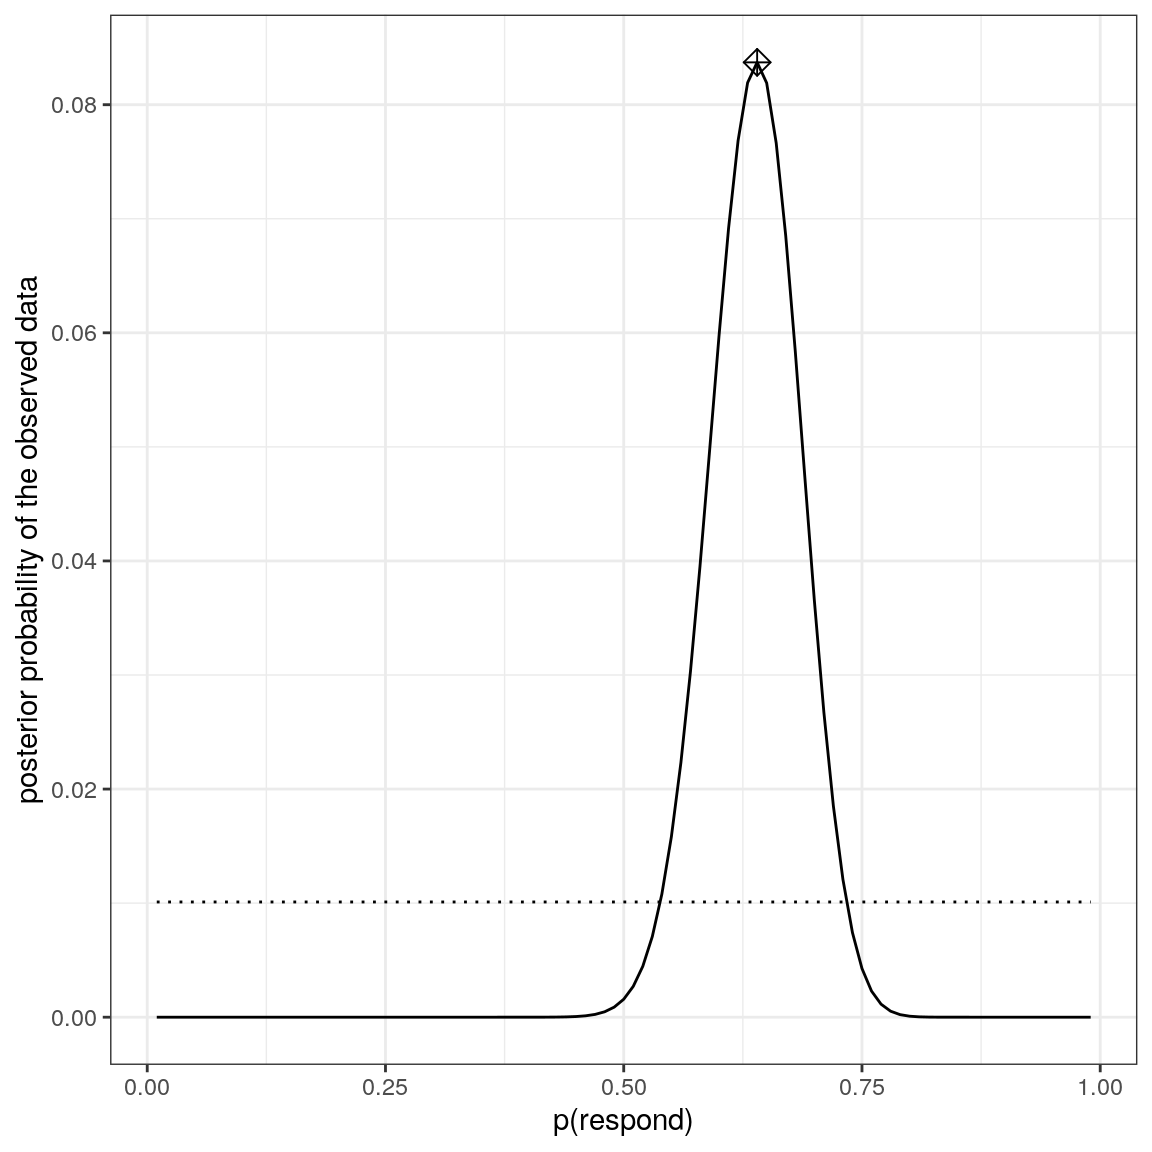
\includegraphics{StatsThinking21_files/figure-latex/unnamed-chunk-142-1.pdf}

\hypertarget{bayes-factors-section-refbayes-factors}{%
\section{Bayes factors (Section \ref{Bayes-factors})}\label{bayes-factors-section-refbayes-factors}}

Example showing how BFs and p-values relate

\hypertarget{modeling-categorical-relationships-in-r}{%
\chapter{Modeling categorical relationships in R}\label{modeling-categorical-relationships-in-r}}

So far we have discussed the general concept of statistical modeling and hypothesis testing, and applied them to some simple analyses. In this chapter we will focus on the modeling of \emph{categorical} relationships, by which we mean relationships between variables that are measured qualitatively. These data are usually expressed in terms of counts; that is, for each value of the variable (or combination of values of multiple variables), how many observations take that value? For example, when we count how many people from each major are in our class, we are fitting a categorical model to the data.

\hypertarget{the-pearson-chi-squared-test-section-refchi-squared-test}{%
\section{The Pearson Chi-squared test (Section \ref{chi-squared-test})}\label{the-pearson-chi-squared-test-section-refchi-squared-test}}

\hypertarget{two-way-tests-section-reftwo-way-test}{%
\section{Two-way tests (Section @ref(two-way-test\})}\label{two-way-tests-section-reftwo-way-test}}

\hypertarget{modeling-continuous-relationships-in-r}{%
\chapter{Modeling continuous relationships in R}\label{modeling-continuous-relationships-in-r}}

\hypertarget{computing-covariance-and-correlation-section-refcovariance-and-correlation}{%
\section{Computing covariance and correlation (Section \ref{covariance-and-correlation})}\label{computing-covariance-and-correlation-section-refcovariance-and-correlation}}

Let's first look at our toy example of covariance and correlation. For this example, we first start by generating a set of X values.

\begin{Shaded}
\begin{Highlighting}[]
\NormalTok{df <-}
\StringTok{  }\KeywordTok{tibble}\NormalTok{(}\DataTypeTok{x =} \KeywordTok{c}\NormalTok{(}\DecValTok{3}\NormalTok{, }\DecValTok{5}\NormalTok{, }\DecValTok{8}\NormalTok{, }\DecValTok{10}\NormalTok{, }\DecValTok{12}\NormalTok{))}
\end{Highlighting}
\end{Shaded}

Then we create a related Y variable by adding some random noise to the X variable:

We compute the deviations and multiply them together to get the crossproduct:

And then we compute the covariance and correlation:

\begin{Shaded}
\begin{Highlighting}[]
\NormalTok{results_df <-}\StringTok{ }\KeywordTok{tibble}\NormalTok{(}
  \DataTypeTok{covXY=}\KeywordTok{sum}\NormalTok{(df}\OperatorTok{$}\NormalTok{crossproduct) }\OperatorTok{/}\StringTok{ }\NormalTok{(}\KeywordTok{nrow}\NormalTok{(df) }\OperatorTok{-}\StringTok{ }\DecValTok{1}\NormalTok{),}
  \DataTypeTok{corXY=} \KeywordTok{sum}\NormalTok{(df}\OperatorTok{$}\NormalTok{crossproduct) }\OperatorTok{/}\StringTok{ }
\StringTok{    }\NormalTok{((}\KeywordTok{nrow}\NormalTok{(df) }\OperatorTok{-}\StringTok{ }\DecValTok{1}\NormalTok{) }\OperatorTok{*}\StringTok{ }\KeywordTok{sd}\NormalTok{(df}\OperatorTok{$}\NormalTok{x) }\OperatorTok{*}\StringTok{ }\KeywordTok{sd}\NormalTok{(df}\OperatorTok{$}\NormalTok{y)))}

\KeywordTok{kable}\NormalTok{(results_df)}
\end{Highlighting}
\end{Shaded}

\begin{tabular}{r|r}
\hline
covXY & corXY\\
\hline
17.05 & 0.894782\\
\hline
\end{tabular}

\hypertarget{hate-crime-example}{%
\section{Hate crime example}\label{hate-crime-example}}

Now we will look at the hate crime data from the \texttt{fivethirtyeight} package. First we need to prepare the data by getting rid of NA values and creating abbreviations for the states. To do the latter, we use the \texttt{state.abb} and \texttt{state.name} variables that come with R along with the \texttt{match()} function that will match the state names in the \texttt{hate\_crimes} variable to those in the list.

\begin{Shaded}
\begin{Highlighting}[]
\NormalTok{hateCrimes <-}\StringTok{ }
\StringTok{  }\NormalTok{hate_crimes }\OperatorTok
\StringTok{  }\KeywordTok{mutate}\NormalTok{(}\DataTypeTok{state_abb =}\NormalTok{ state.abb[}\KeywordTok{match}\NormalTok{(state,state.name)]) }\OperatorTok
\StringTok{  }\KeywordTok{drop_na}\NormalTok{(avg_hatecrimes_per_100k_fbi, gini_index)}

\CommentTok{# manually fix the DC abbreviation}
\NormalTok{hateCrimes}\OperatorTok{$}\NormalTok{state_abb[hateCrimes}\OperatorTok{$}\NormalTok{state}\OperatorTok{==}\StringTok{"District of Columbia"}\NormalTok{] <-}\StringTok{ 'DC'}
\end{Highlighting}
\end{Shaded}

\begin{verbatim}
## 
##  Pearson's product-moment correlation
## 
## data:  hateCrimes$avg_hatecrimes_per_100k_fbi and hateCrimes$gini_index
## t = 3.2182, df = 48, p-value = 0.001157
## alternative hypothesis: true correlation is greater than 0
## 95 percent confidence interval:
##  0.2063067 1.0000000
## sample estimates:
##       cor 
## 0.4212719
\end{verbatim}

Remember that we can also compute the p-value using randomization. To to this, we shuffle the order of one of the variables, so that we break the link between the X and Y variables --- effectively making the null hypothesis (that the correlation is less than or equal to zero) true. Here we will first create a function that takes in two variables, shuffles the order of one of them (without replacement) and then returns the correlation between that shuffled variable and the original copy of the second variable.

Now we take the distribution of observed correlations after shuffling and compare them to our observed correlation, in order to obtain the empirical probability of our observed data under the null hypothesis.

\begin{Shaded}
\begin{Highlighting}[]
\KeywordTok{mean}\NormalTok{(shuffleDist}\OperatorTok{$}\NormalTok{cor }\OperatorTok{>}\NormalTok{corr_results}\OperatorTok{$}\NormalTok{estimate )}
\end{Highlighting}
\end{Shaded}

\begin{verbatim}
## [1] 0.0066
\end{verbatim}

This value is fairly close (though a bit larger) to the one obtained using \texttt{cor.test()}.

\hypertarget{robust-correlations-section-refrobust-correlations}{%
\section{Robust correlations (Section \ref{robust-correlations})}\label{robust-correlations-section-refrobust-correlations}}

In the previous chapter we also saw that the hate crime data contained one substantial outlier, which appeared to drive the significant correlation. To compute the Spearman correlation, we first need to convert the data into their ranks, which we can do using the \texttt{order()} function:

\begin{Shaded}
\begin{Highlighting}[]
\NormalTok{hateCrimes <-}\StringTok{ }\NormalTok{hateCrimes }\OperatorTok
\StringTok{  }\KeywordTok{mutate}\NormalTok{(}\DataTypeTok{hatecrimes_rank =} \KeywordTok{order}\NormalTok{(avg_hatecrimes_per_100k_fbi),}
         \DataTypeTok{gini_rank =} \KeywordTok{order}\NormalTok{(gini_index))}
\end{Highlighting}
\end{Shaded}

We can then compute the Spearman correlation by applying the Pearson correlation to the rank variables"

\begin{Shaded}
\begin{Highlighting}[]
\KeywordTok{cor}\NormalTok{(hateCrimes}\OperatorTok{$}\NormalTok{hatecrimes_rank,}
\NormalTok{  hateCrimes}\OperatorTok{$}\NormalTok{gini_rank)}
\end{Highlighting}
\end{Shaded}

\begin{verbatim}
## [1] 0.05690276
\end{verbatim}

We see that this is much smaller than the value obtained using the Pearson correlation on the original data. We can assess its statistical signficance using randomization:

\begin{verbatim}
## [1] 0.0014
\end{verbatim}

Here we see that the p-value is substantially larger and far from significance.

\hypertarget{the-general-linear-model-in-r}{%
\chapter{The General Linear Model in R}\label{the-general-linear-model-in-r}}

\hypertarget{linear-regression-section-reflinear-regression}{%
\section{Linear regression (Section \ref{linear-regression})}\label{linear-regression-section-reflinear-regression}}

To perform linear regression in R, we use the \texttt{lm()} function. Let's generate some data and use this function to compute the linear regression solution.

\begin{Shaded}
\begin{Highlighting}[]
\NormalTok{npoints <-}\StringTok{ }\DecValTok{100}
\NormalTok{intercept =}\StringTok{ }\DecValTok{10}
\CommentTok{# slope of X/Y relationship}
\NormalTok{slope=}\FloatTok{0.5}
\CommentTok{# this lets us control the strength of the relationship}
\CommentTok{# by varying the amount of noise added to the y variable}
\NormalTok{noise_sd =}\StringTok{ }\FloatTok{0.6}

\NormalTok{regression_data <-}\StringTok{ }\KeywordTok{tibble}\NormalTok{(}\DataTypeTok{x =} \KeywordTok{rnorm}\NormalTok{(npoints)) }\OperatorTok
\StringTok{  }\KeywordTok{mutate}\NormalTok{(}\DataTypeTok{y =}\NormalTok{ x}\OperatorTok{*}\NormalTok{slope }\OperatorTok{+}\StringTok{ }\KeywordTok{rnorm}\NormalTok{(npoints)}\OperatorTok{*}\NormalTok{noise_sd }\OperatorTok{+}\StringTok{ }\NormalTok{intercept)}

\KeywordTok{ggplot}\NormalTok{(regression_data,}\KeywordTok{aes}\NormalTok{(x,y)) }\OperatorTok{+}\StringTok{ }
\StringTok{  }\KeywordTok{geom_point}\NormalTok{()}
\end{Highlighting}
\end{Shaded}

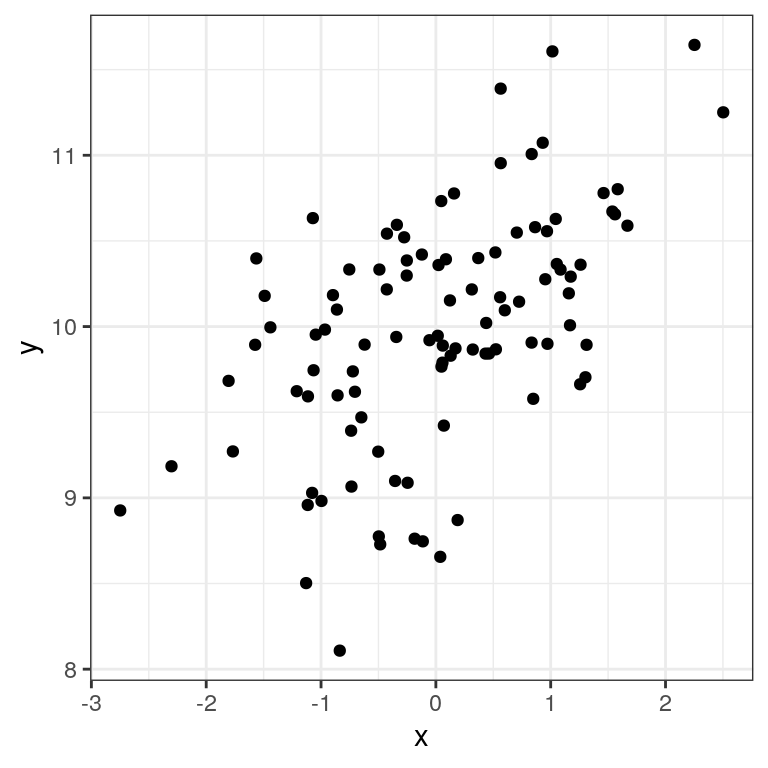
\includegraphics[width=0.5\linewidth]{StatsThinking21_files/figure-latex/unnamed-chunk-159-1}

We can then apply \texttt{lm()} to these data:

\begin{Shaded}
\begin{Highlighting}[]
\NormalTok{lm_result <-}\StringTok{ }\KeywordTok{lm}\NormalTok{(y }\OperatorTok{~}\StringTok{ }\NormalTok{x, }\DataTypeTok{data=}\NormalTok{regression_data)}
\KeywordTok{summary}\NormalTok{(lm_result)}
\end{Highlighting}
\end{Shaded}

\begin{verbatim}
## 
## Call:
## lm(formula = y ~ x, data = regression_data)
## 
## Residuals:
##      Min       1Q   Median       3Q      Max 
## -1.55632 -0.30424 -0.00587  0.38039  1.25219 
## 
## Coefficients:
##             Estimate Std. Error t value Pr(>|t|)    
## (Intercept)  9.97610    0.05796 172.122  < 2e-16 ***
## x            0.37246    0.05862   6.353 6.65e-09 ***
## ---
## Signif. codes:  0 '***' 0.001 '**' 0.01 '*' 0.05 '.' 0.1 ' ' 1
## 
## Residual standard error: 0.5795 on 98 degrees of freedom
## Multiple R-squared:  0.2917, Adjusted R-squared:  0.2845 
## F-statistic: 40.36 on 1 and 98 DF,  p-value: 6.646e-09
\end{verbatim}

We should see three things in the \texttt{lm()} results:

\begin{itemize}
\tightlist
\item
  The estimate of the Intercept in the model should be very close to the intercept that we specified
\item
  The estimate for the x parameter should be very close to the slope that we specified
\item
  The residual standard error should be roughly similar to the noise standard deviation that we specified
\end{itemize}

\hypertarget{model-criticism-and-diagnostics-section-refmodel-criticism}{%
\section{Model criticism and diagnostics (Section \ref{model-criticism})}\label{model-criticism-and-diagnostics-section-refmodel-criticism}}

Once we have fitted the model, we want to look at some diagnostics to determine whether the model is actually fitting properly. We can do this using the \texttt{autoplot()} function from the \texttt{ggfortify} package.

\begin{Shaded}
\begin{Highlighting}[]
\KeywordTok{autoplot}\NormalTok{(lm_result,}\DataTypeTok{which=}\DecValTok{1}\OperatorTok{:}\DecValTok{2}\NormalTok{)}
\end{Highlighting}
\end{Shaded}

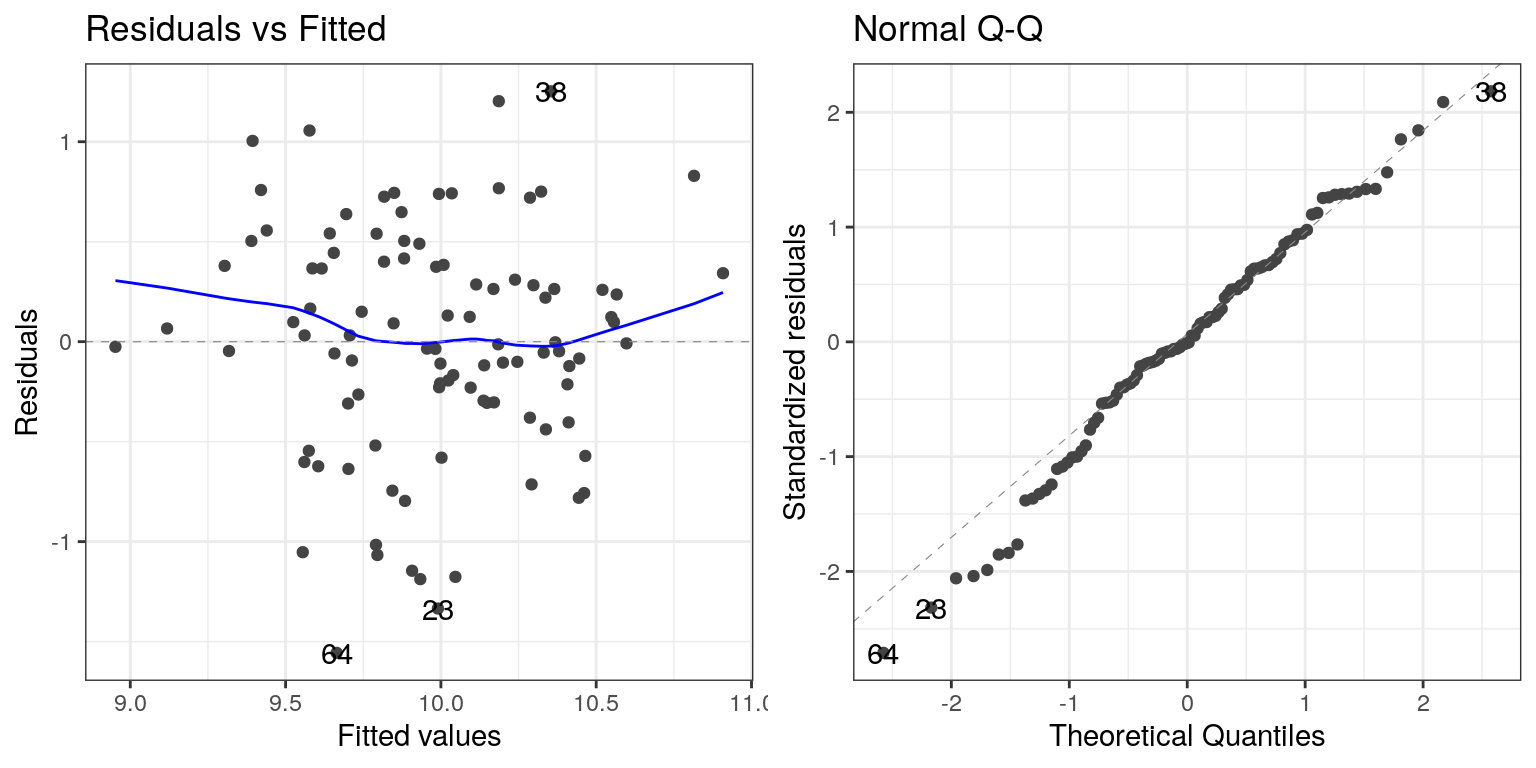
\includegraphics[width=0.8\linewidth]{StatsThinking21_files/figure-latex/unnamed-chunk-161-1}

The left panel in this plot shows the relationship between the predicted (or ``fitted'') values and the residuals. We would like to make sure that there is no clear relationship between these two (as we will see below). The right panel shows a Q-Q plot, which helps us assess whether the residuals from the model are normally distributed. In this case, they look reasonably normal, as the points don't differ too much from the unit line.

\hypertarget{examples-of-problematic-model-fit}{%
\section{Examples of problematic model fit}\label{examples-of-problematic-model-fit}}

Let's say that there was another variable at play in this dataset, which we were not aware of. This variable causes some of the cases to have much larger values than others, in a way that is unrelated to the X variable. We play a trick here using the \texttt{seq()} function to create a sequence from zero to one, and then threshold those 0.5 (in order to obtain half of the values as zero and the other half as one) and then multiply by the desired effect size:

\begin{Shaded}
\begin{Highlighting}[]
\NormalTok{effsize=}\DecValTok{2}
\NormalTok{regression_data <-}\StringTok{ }\NormalTok{regression_data }\OperatorTok
\StringTok{  }\KeywordTok{mutate}\NormalTok{(}\DataTypeTok{y2=}\NormalTok{y }\OperatorTok{+}\StringTok{ }\NormalTok{effsize}\OperatorTok{*}\NormalTok{(}\KeywordTok{seq}\NormalTok{(}\DecValTok{1}\OperatorTok{/}\NormalTok{npoints,}\DecValTok{1}\NormalTok{,}\DecValTok{1}\OperatorTok{/}\NormalTok{npoints)}\OperatorTok{>}\FloatTok{0.5}\NormalTok{))}

\NormalTok{lm_result2 <-}\StringTok{ }\KeywordTok{lm}\NormalTok{(y2 }\OperatorTok{~}\StringTok{ }\NormalTok{x, }\DataTypeTok{data=}\NormalTok{regression_data)}
\KeywordTok{summary}\NormalTok{(lm_result2)}
\end{Highlighting}
\end{Shaded}

\begin{verbatim}
## 
## Call:
## lm(formula = y2 ~ x, data = regression_data)
## 
## Residuals:
##      Min       1Q   Median       3Q      Max 
## -2.33243 -0.96887 -0.09385  1.04213  2.25913 
## 
## Coefficients:
##             Estimate Std. Error t value Pr(>|t|)    
## (Intercept)  10.9778     0.1172  93.646   <2e-16 ***
## x             0.2696     0.1186   2.273   0.0252 *  
## ---
## Signif. codes:  0 '***' 0.001 '**' 0.01 '*' 0.05 '.' 0.1 ' ' 1
## 
## Residual standard error: 1.172 on 98 degrees of freedom
## Multiple R-squared:  0.0501, Adjusted R-squared:  0.04041 
## F-statistic: 5.169 on 1 and 98 DF,  p-value: 0.02518
\end{verbatim}

One thing you should notice is that the model now fits overall much worse; the R-squared is about half of what it was in the previous model, which reflects the fact that more variability was added to the data, but it wasn't accounted for in the model. Let's see if our diagnostic reports can give us any insight:

\begin{Shaded}
\begin{Highlighting}[]
\KeywordTok{autoplot}\NormalTok{(lm_result2,}\DataTypeTok{which=}\DecValTok{1}\OperatorTok{:}\DecValTok{2}\NormalTok{)}
\end{Highlighting}
\end{Shaded}

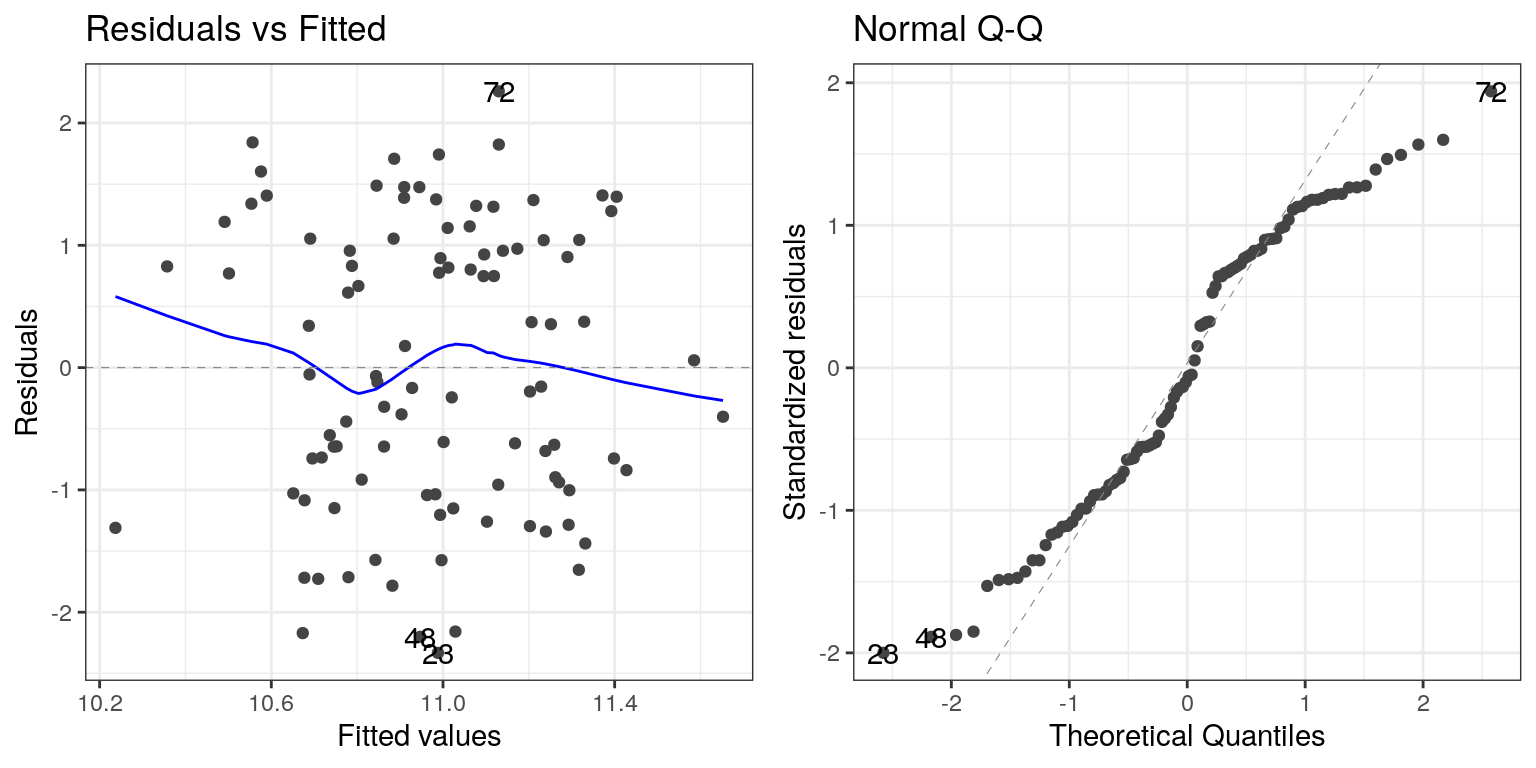
\includegraphics[width=0.8\linewidth]{StatsThinking21_files/figure-latex/unnamed-chunk-163-1}

The residual versus fitted graph doesn't give us much insight, but we see from the Q-Q plot that the residuals are diverging quite a bit from the unit line.

Let's look at another potential problem, in which the y variable is nonlinearly related to the X variable. We can create these data by squaring the X variable when we generate the Y variable:

\begin{Shaded}
\begin{Highlighting}[]
\NormalTok{effsize=}\DecValTok{2}
\NormalTok{regression_data <-}\StringTok{ }\NormalTok{regression_data }\OperatorTok
\StringTok{  }\KeywordTok{mutate}\NormalTok{(}\DataTypeTok{y3 =}\NormalTok{ (x}\OperatorTok{**}\DecValTok{2}\NormalTok{)}\OperatorTok{*}\NormalTok{slope }\OperatorTok{+}\StringTok{ }\KeywordTok{rnorm}\NormalTok{(npoints)}\OperatorTok{*}\NormalTok{noise_sd }\OperatorTok{+}\StringTok{ }\NormalTok{intercept)}

\NormalTok{lm_result3 <-}\StringTok{ }\KeywordTok{lm}\NormalTok{(y3 }\OperatorTok{~}\StringTok{ }\NormalTok{x, }\DataTypeTok{data=}\NormalTok{regression_data)}
\KeywordTok{summary}\NormalTok{(lm_result3)}
\end{Highlighting}
\end{Shaded}

\begin{verbatim}
## 
## Call:
## lm(formula = y3 ~ x, data = regression_data)
## 
## Residuals:
##     Min      1Q  Median      3Q     Max 
## -1.6100 -0.5679 -0.0649  0.3587  3.2662 
## 
## Coefficients:
##             Estimate Std. Error t value Pr(>|t|)    
## (Intercept) 10.55467    0.08439 125.073   <2e-16 ***
## x           -0.04189    0.08536  -0.491    0.625    
## ---
## Signif. codes:  0 '***' 0.001 '**' 0.01 '*' 0.05 '.' 0.1 ' ' 1
## 
## Residual standard error: 0.8438 on 98 degrees of freedom
## Multiple R-squared:  0.002452,   Adjusted R-squared:  -0.007727 
## F-statistic: 0.2409 on 1 and 98 DF,  p-value: 0.6247
\end{verbatim}

Now we see that there is no significant linear relationship between \(X^2\) and Y/ But if we look at the residuals the problem with the model becomes clear:

\begin{Shaded}
\begin{Highlighting}[]
\KeywordTok{autoplot}\NormalTok{(lm_result3,}\DataTypeTok{which=}\DecValTok{1}\OperatorTok{:}\DecValTok{2}\NormalTok{)}
\end{Highlighting}
\end{Shaded}

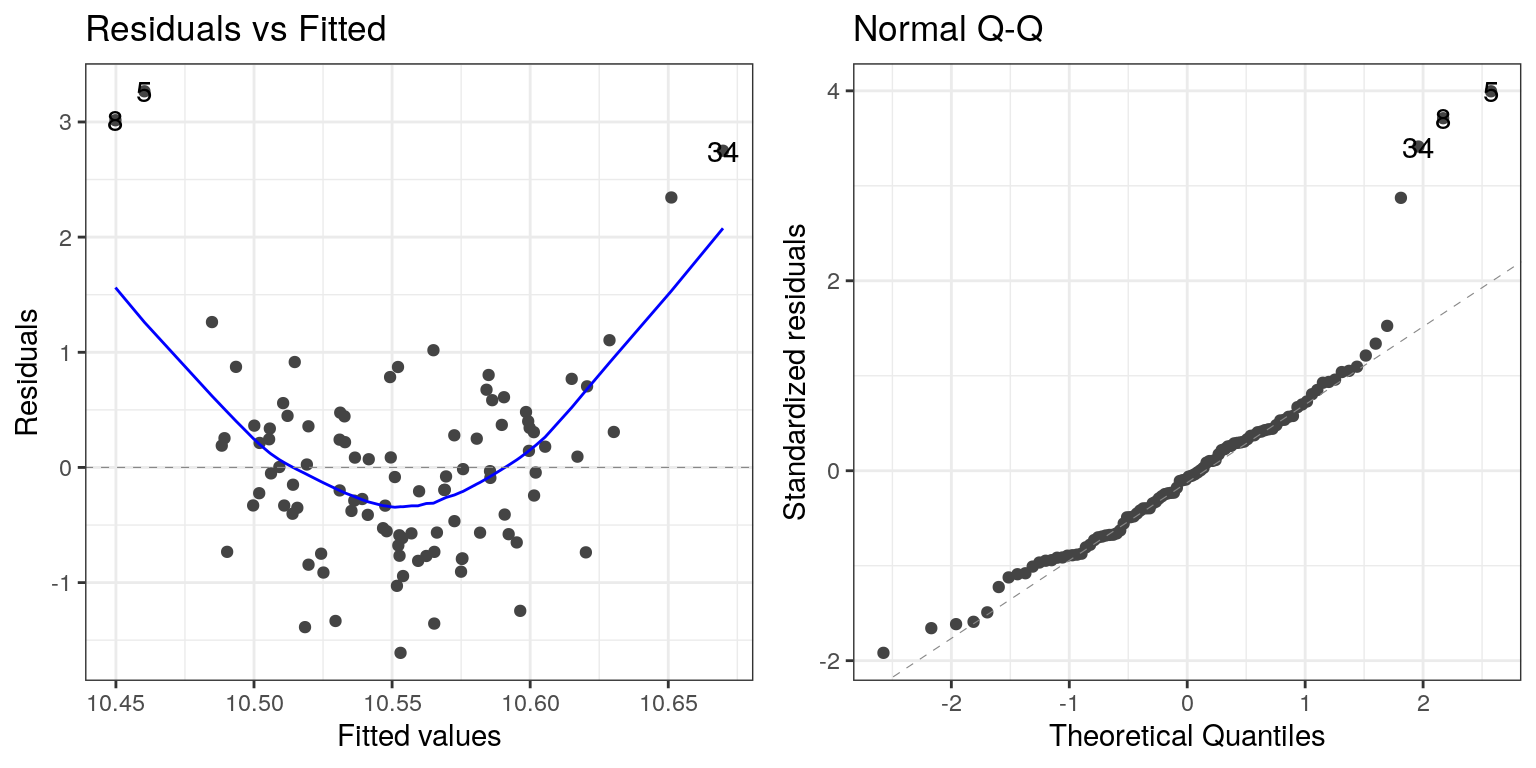
\includegraphics[width=0.8\linewidth]{StatsThinking21_files/figure-latex/unnamed-chunk-165-1}

In this case we can see the clearly nonlinear relationship between the predicted and residual values, as well as the clear lack of normality in the residuals.

As we noted in the previous chapter, the ``linear'' in the general linear model doesn't refer to the shape of the response, but instead refers to the fact that model is linear in its parameters --- that is, the predictors in the model only get multiplied the parameters (e.g., rather than being raised to a power of the parameter). Here is how we would build a model that could account for the nonlinear relationship:

\begin{Shaded}
\begin{Highlighting}[]
\CommentTok{# create x^2 variable}
\NormalTok{regression_data <-}\StringTok{ }\NormalTok{regression_data }\OperatorTok
\StringTok{  }\KeywordTok{mutate}\NormalTok{(}\DataTypeTok{x_squared =}\NormalTok{ x}\OperatorTok{**}\DecValTok{2}\NormalTok{)}

\NormalTok{lm_result4 <-}\StringTok{ }\KeywordTok{lm}\NormalTok{(y3 }\OperatorTok{~}\StringTok{ }\NormalTok{x }\OperatorTok{+}\StringTok{ }\NormalTok{x_squared, }\DataTypeTok{data=}\NormalTok{regression_data)}
\KeywordTok{summary}\NormalTok{(lm_result4)}
\end{Highlighting}
\end{Shaded}

\begin{verbatim}
## 
## Call:
## lm(formula = y3 ~ x + x_squared, data = regression_data)
## 
## Residuals:
##      Min       1Q   Median       3Q      Max 
## -1.41009 -0.37915 -0.00483  0.39079  1.44368 
## 
## Coefficients:
##             Estimate Std. Error t value Pr(>|t|)    
## (Intercept) 10.10875    0.07387 136.836   <2e-16 ***
## x           -0.01178    0.05998  -0.196    0.845    
## x_squared    0.45569    0.04513  10.098   <2e-16 ***
## ---
## Signif. codes:  0 '***' 0.001 '**' 0.01 '*' 0.05 '.' 0.1 ' ' 1
## 
## Residual standard error: 0.5922 on 97 degrees of freedom
## Multiple R-squared:  0.5137, Adjusted R-squared:  0.5037 
## F-statistic: 51.23 on 2 and 97 DF,  p-value: 6.536e-16
\end{verbatim}

Now we see that the effect of \(X^2\) is significant, and if we look at the residual plot we should see that things look much better:

\begin{Shaded}
\begin{Highlighting}[]
\KeywordTok{autoplot}\NormalTok{(lm_result4,}\DataTypeTok{which=}\DecValTok{1}\OperatorTok{:}\DecValTok{2}\NormalTok{)}
\end{Highlighting}
\end{Shaded}

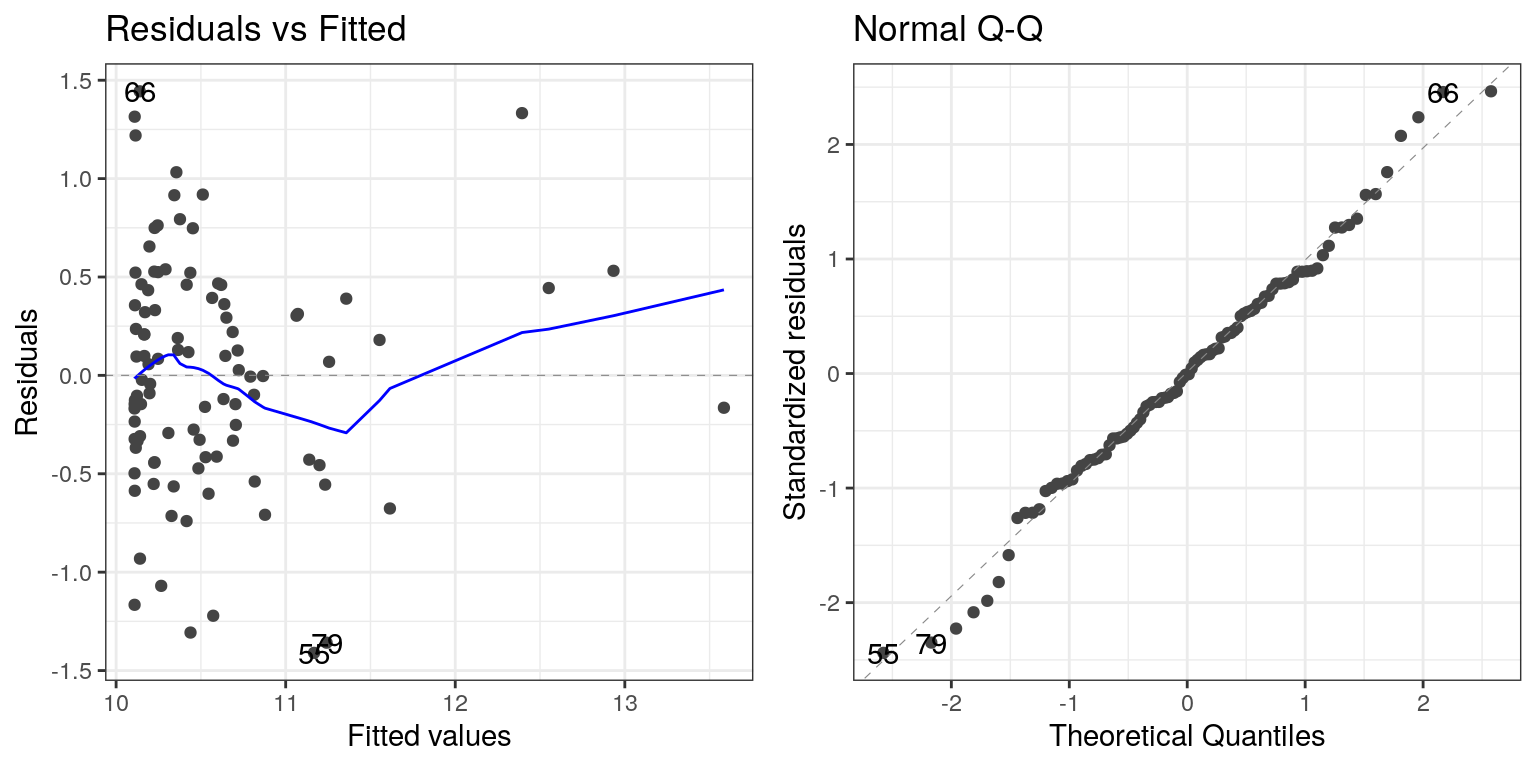
\includegraphics[width=0.8\linewidth]{StatsThinking21_files/figure-latex/unnamed-chunk-167-1}
Not perfect, but much better than before!

\hypertarget{extending-regression-to-binary-outcomes.}{%
\section{Extending regression to binary outcomes.}\label{extending-regression-to-binary-outcomes.}}

Let's say that we have a blood test (which is often referred to as a \emph{biomarker}) and we want to know whether it predicts who is going to have a heart attack within the next year. We will generate a synthetic dataset for a population that is at very high risk for a heart attack in the next year.

\begin{Shaded}
\begin{Highlighting}[]
\CommentTok{# sample size}
\NormalTok{npatients=}\DecValTok{1000}

\CommentTok{# probability of heart attack}
\NormalTok{p_heartattack =}\StringTok{ }\FloatTok{0.5}

\CommentTok{# true relation to biomarker}
\NormalTok{true_effect <-}\StringTok{ }\FloatTok{0.6}

\CommentTok{# assume biomarker is normally distributed}
\NormalTok{disease_df <-}\StringTok{ }\KeywordTok{tibble}\NormalTok{(}\DataTypeTok{biomarker=}\KeywordTok{rnorm}\NormalTok{(npatients))}

\CommentTok{# generate another variable that reflects risk for }
\CommentTok{# heart attack, which is related to the biomarker}
\NormalTok{disease_df <-}\StringTok{ }\NormalTok{disease_df }\OperatorTok
\StringTok{  }\KeywordTok{mutate}\NormalTok{(}\DataTypeTok{risk =}\NormalTok{ biomarker}\OperatorTok{*}\NormalTok{true_effect }\OperatorTok{+}\StringTok{ }\KeywordTok{rnorm}\NormalTok{(npatients))}

\CommentTok{# create another variable that shows who has a }
\CommentTok{# heart attack, based on the risk variable}
\NormalTok{disease_df <-}\StringTok{ }\NormalTok{disease_df }\OperatorTok
\StringTok{  }\KeywordTok{mutate}\NormalTok{(}
    \DataTypeTok{heartattack =}\NormalTok{ risk }\OperatorTok{>}\StringTok{ }\KeywordTok{quantile}\NormalTok{(disease_df}\OperatorTok{$}\NormalTok{risk,}
                                       \DecValTok{1}\OperatorTok{-}\NormalTok{p_heartattack))}

\KeywordTok{glimpse}\NormalTok{(disease_df)}
\end{Highlighting}
\end{Shaded}

\begin{verbatim}
## Observations: 1,000
## Variables: 3
## $ biomarker   <dbl> 1.1512317, 0.6753651, 1.2141696, -0...
## $ risk        <dbl> 1.05356169, -0.52889832, 0.67528209...
## $ heartattack <lgl> TRUE, FALSE, TRUE, FALSE, FALSE, TR...
\end{verbatim}

Now we would like to build a model that allows us to predict who will have a heart attack from these data. However, you may have noticed that the heartattack variable is a binary variable; because linear regression assumes that the residuals from the model will be normally distributed, and the binary nature of the data will violate this, we instead need to use a different kind of model, known as a \emph{logistic regression} model, which is built to deal with binary outcomes. We can fit this model using the \texttt{glm()} function:

\begin{Shaded}
\begin{Highlighting}[]
\NormalTok{glm_result <-}\StringTok{ }\KeywordTok{glm}\NormalTok{(heartattack }\OperatorTok{~}\StringTok{ }\NormalTok{biomarker, }\DataTypeTok{data=}\NormalTok{disease_df,}
                  \DataTypeTok{family=}\KeywordTok{binomial}\NormalTok{())}
\KeywordTok{summary}\NormalTok{(glm_result)}
\end{Highlighting}
\end{Shaded}

\begin{verbatim}
## 
## Call:
## glm(formula = heartattack ~ biomarker, family = binomial(), data = disease_df)
## 
## Deviance Residuals: 
##      Min        1Q    Median        3Q       Max  
## -2.13007  -1.01501   0.03054   1.00492   2.13191  
## 
## Coefficients:
##              Estimate Std. Error z value Pr(>|z|)    
## (Intercept) -0.004117   0.069479  -0.059    0.953    
## biomarker    0.996366   0.083418  11.944   <2e-16 ***
## ---
## Signif. codes:  0 '***' 0.001 '**' 0.01 '*' 0.05 '.' 0.1 ' ' 1
## 
## (Dispersion parameter for binomial family taken to be 1)
## 
##     Null deviance: 1386.3  on 999  degrees of freedom
## Residual deviance: 1201.4  on 998  degrees of freedom
## AIC: 1205.4
## 
## Number of Fisher Scoring iterations: 3
\end{verbatim}

This looks very similar to the output from the \texttt{lm()} function, and it shows us that there is a significant relationship between the biomarker and heart attacks. The model provides us with a predicted probability that each individual will have a heart attack; if this is greater than 0.5, then that means that the model predicts that the individual is more likely than not to have a heart attack.\\
We can start by simply comparing those predictions to the actual outcomes.

\begin{Shaded}
\begin{Highlighting}[]
\CommentTok{# add predictions to data frame}
\NormalTok{disease_df <-}\StringTok{ }\NormalTok{disease_df }\OperatorTok
\StringTok{  }\KeywordTok{mutate}\NormalTok{(}\DataTypeTok{prediction =}\NormalTok{ glm_result}\OperatorTok{$}\NormalTok{fitted.values}\OperatorTok{>}\FloatTok{0.5}\NormalTok{,}
         \DataTypeTok{heartattack =}\NormalTok{ heartattack)}

\CommentTok{# create table comparing predicted to actual outcomes}
\KeywordTok{CrossTable}\NormalTok{(disease_df}\OperatorTok{$}\NormalTok{prediction,}
\NormalTok{           disease_df}\OperatorTok{$}\NormalTok{heartattack,}
           \DataTypeTok{prop.t=}\OtherTok{FALSE}\NormalTok{,}
           \DataTypeTok{prop.r=}\OtherTok{FALSE}\NormalTok{,}
           \DataTypeTok{prop.chisq=}\OtherTok{FALSE}\NormalTok{)}
\end{Highlighting}
\end{Shaded}

\begin{verbatim}
## 
##  
##    Cell Contents
## |-------------------------|
## |                       N |
## |           N / Col Total |
## |-------------------------|
## 
##  
## Total Observations in Table:  1000 
## 
##  
##                       | disease_df$heartattack 
## disease_df$prediction |     FALSE |      TRUE | Row Total | 
## ----------------------|-----------|-----------|-----------|
##                 FALSE |       332 |       157 |       489 | 
##                       |     0.664 |     0.314 |           | 
## ----------------------|-----------|-----------|-----------|
##                  TRUE |       168 |       343 |       511 | 
##                       |     0.336 |     0.686 |           | 
## ----------------------|-----------|-----------|-----------|
##          Column Total |       500 |       500 |      1000 | 
##                       |     0.500 |     0.500 |           | 
## ----------------------|-----------|-----------|-----------|
## 
## 
\end{verbatim}

This shows us that of the 500 people who had heart attacks, the model corrected predicted a heart attack for 343 of them. It also predicted heart attacks for 168 people who didn't have them, and it failed to predict a heart attack for 157 people who had them. This highlights the distinction that we mentioned before between statistical and practical significance; even though the biomarker shows a highly significant relationship to heart attacks, it's ability to predict them is still relatively poor. As we will see below, it gets even worse when we try to generalize this to a new group of people.

\hypertarget{cross-validation-section-refcross-validation}{%
\section{Cross-validation (Section \ref{cross-validation})}\label{cross-validation-section-refcross-validation}}

Cross-validation is a powerful technique that allows us to estimate how well our results will generalize to a new dataset. Here we will build our own crossvalidation code to see how it works, continuing the logistic regression example from the previous section.

In cross-validation, we want to split the data into several subsets and then iteratively train the model while leaving out each subset (which we usually call \emph{folds}) and then test the model on that held-out fold Let's write our own code to do this splitting; one relatively easy way to this is to create a vector that contains the fold numbers, and then randomly shuffle it to create the fold assigments for each data point.

\begin{Shaded}
\begin{Highlighting}[]
\NormalTok{nfolds <-}\StringTok{ }\DecValTok{4} \CommentTok{# number of folds}

\CommentTok{# we use the kronecker() function to repeat the folds}
\NormalTok{fold <-}\StringTok{  }\KeywordTok{kronecker}\NormalTok{(}\KeywordTok{seq}\NormalTok{(nfolds),}\KeywordTok{rep}\NormalTok{(}\DecValTok{1}\NormalTok{,npatients}\OperatorTok{/}\NormalTok{nfolds))}
\CommentTok{# randomly shuffle using the sample() function}
\NormalTok{fold <-}\StringTok{ }\KeywordTok{sample}\NormalTok{(fold)}

\CommentTok{# add variable to store CV predictions}
\NormalTok{disease_df <-}\StringTok{ }\NormalTok{disease_df }\OperatorTok
\StringTok{  }\KeywordTok{mutate}\NormalTok{(}\DataTypeTok{CVpred=}\OtherTok{NA}\NormalTok{)}

\CommentTok{# now loop through folds and separate training and test data}
\ControlFlowTok{for}\NormalTok{ (f }\ControlFlowTok{in} \KeywordTok{seq}\NormalTok{(nfolds))\{}
  \CommentTok{# get training and test data}
\NormalTok{  train_df <-}\StringTok{ }\NormalTok{disease_df[fold}\OperatorTok{!=}\NormalTok{f,]}
\NormalTok{  test_df <-}\StringTok{ }\NormalTok{disease_df[fold}\OperatorTok{==}\NormalTok{f,]}
  \CommentTok{# fit model to training data}
\NormalTok{  glm_result_cv <-}\StringTok{ }\KeywordTok{glm}\NormalTok{(heartattack }\OperatorTok{~}\StringTok{ }\NormalTok{biomarker, }\DataTypeTok{data=}\NormalTok{train_df,}
                  \DataTypeTok{family=}\KeywordTok{binomial}\NormalTok{())}
  \CommentTok{# get probability of heart attack on test data}
\NormalTok{  pred <-}\StringTok{ }\KeywordTok{predict}\NormalTok{(glm_result_cv,}\DataTypeTok{newdata =}\NormalTok{ test_df)}
  \CommentTok{# convert to prediction and put into data frame}
\NormalTok{  disease_df}\OperatorTok{$}\NormalTok{CVpred[fold}\OperatorTok{==}\NormalTok{f] =}\StringTok{ }\NormalTok{(pred}\OperatorTok{>}\FloatTok{0.5}\NormalTok{)}

\NormalTok{\}}
\end{Highlighting}
\end{Shaded}

Now let's look at the performance of the model:

\begin{Shaded}
\begin{Highlighting}[]
\CommentTok{# create table comparing predicted to actual outcomes}
\KeywordTok{CrossTable}\NormalTok{(disease_df}\OperatorTok{$}\NormalTok{CVpred,}
\NormalTok{           disease_df}\OperatorTok{$}\NormalTok{heartattack,}
           \DataTypeTok{prop.t=}\OtherTok{FALSE}\NormalTok{,}
           \DataTypeTok{prop.r=}\OtherTok{FALSE}\NormalTok{,}
           \DataTypeTok{prop.chisq=}\OtherTok{FALSE}\NormalTok{)}
\end{Highlighting}
\end{Shaded}

\begin{verbatim}
## 
##  
##    Cell Contents
## |-------------------------|
## |                       N |
## |           N / Col Total |
## |-------------------------|
## 
##  
## Total Observations in Table:  1000 
## 
##  
##                   | disease_df$heartattack 
## disease_df$CVpred |     FALSE |      TRUE | Row Total | 
## ------------------|-----------|-----------|-----------|
##             FALSE |       416 |       269 |       685 | 
##                   |     0.832 |     0.538 |           | 
## ------------------|-----------|-----------|-----------|
##              TRUE |        84 |       231 |       315 | 
##                   |     0.168 |     0.462 |           | 
## ------------------|-----------|-----------|-----------|
##      Column Total |       500 |       500 |      1000 | 
##                   |     0.500 |     0.500 |           | 
## ------------------|-----------|-----------|-----------|
## 
## 
\end{verbatim}

Now we see that the model only accurately predicts less than half of the heart attacks that occurred when it is predicting to a new sample. This tells us that this is the level of prediction that we could expect if were to apply the model to a new sample of patients from the same population.

\hypertarget{comparing-means-in-r}{%
\chapter{Comparing means in R}\label{comparing-means-in-r}}

\hypertarget{testing-the-value-of-a-single-mean-section-refsingle-mean}{%
\section{Testing the value of a single mean (Section \ref{single-mean})}\label{testing-the-value-of-a-single-mean-section-refsingle-mean}}

In this example, we will show multiple ways to test a hypothesis about the value of a single mean. As an example, let's test whether the mean systolic blood pressure (BP) in the NHANES dataset (averaged over the three measurements that were taken for each person) is greater than 120 mm, which is the standard value for normal systolic BP.

First let's perform a power analysis to see how large our sample would need to be in order to detect a small difference (Cohen's d = .2).

\begin{Shaded}
\begin{Highlighting}[]
\NormalTok{pwr.result <-}\StringTok{ }\KeywordTok{pwr.t.test}\NormalTok{(}\DataTypeTok{d=}\FloatTok{0.2}\NormalTok{, }\DataTypeTok{power=}\FloatTok{0.8}\NormalTok{, }
           \DataTypeTok{type=}\StringTok{'one.sample'}\NormalTok{, }
           \DataTypeTok{alternative=}\StringTok{'greater'}\NormalTok{)}
\NormalTok{pwr.result}
\end{Highlighting}
\end{Shaded}

\begin{verbatim}
## 
##      One-sample t test power calculation 
## 
##               n = 155.9256
##               d = 0.2
##       sig.level = 0.05
##           power = 0.8
##     alternative = greater
\end{verbatim}

Based on this, we take a sample of 156 individuals from the dataset.

\begin{Shaded}
\begin{Highlighting}[]
\NormalTok{NHANES_BP_sample <-}\StringTok{ }\NormalTok{NHANES_adult }\OperatorTok
\StringTok{  }\KeywordTok{drop_na}\NormalTok{(BPSysAve) }\OperatorTok
\StringTok{  }\NormalTok{dplyr}\OperatorTok{::}\KeywordTok{select}\NormalTok{(BPSysAve) }\OperatorTok
\StringTok{  }\KeywordTok{sample_n}\NormalTok{(pwr.result}\OperatorTok{$}\NormalTok{n)}

\KeywordTok{print}\NormalTok{(}\StringTok{'Mean BP:'}\NormalTok{)}
\end{Highlighting}
\end{Shaded}

\begin{verbatim}
## [1] "Mean BP:"
\end{verbatim}

\begin{Shaded}
\begin{Highlighting}[]
\NormalTok{meanBP <-}\StringTok{ }\NormalTok{NHANES_BP_sample }\OperatorTok
\StringTok{  }\KeywordTok{summarize}\NormalTok{(}\DataTypeTok{meanBP=}\KeywordTok{mean}\NormalTok{(BPSysAve)) }\OperatorTok
\StringTok{  }\KeywordTok{pull}\NormalTok{()}
\NormalTok{meanBP}
\end{Highlighting}
\end{Shaded}

\begin{verbatim}
## [1] 123.1097
\end{verbatim}

First let's perform a sign test to see whether the observed mean of 123.11 is significantly different from zero. To do this, we count the number of values that are greater than the hypothesized mean, and then use a binomial test to ask how surprising that number is if the true proportion is 0.5 (as it would be if the distribution were centered at the hypothesized mean).

\begin{Shaded}
\begin{Highlighting}[]
\NormalTok{NHANES_BP_sample <-}\StringTok{ }\NormalTok{NHANES_BP_sample }\OperatorTok
\StringTok{  }\KeywordTok{mutate}\NormalTok{(}\DataTypeTok{BPover120=}\NormalTok{BPSysAve}\OperatorTok{>}\DecValTok{120}\NormalTok{)}

\NormalTok{nOver120 <-}\StringTok{ }\NormalTok{NHANES_BP_sample }\OperatorTok
\StringTok{  }\KeywordTok{summarize}\NormalTok{(}\DataTypeTok{nOver120=}\KeywordTok{sum}\NormalTok{(BPover120)) }\OperatorTok
\StringTok{  }\KeywordTok{pull}\NormalTok{()}

\KeywordTok{binom.test}\NormalTok{(nOver120, }\KeywordTok{nrow}\NormalTok{(NHANES_BP_sample), }\DataTypeTok{alternative=}\StringTok{'greater'}\NormalTok{)}
\end{Highlighting}
\end{Shaded}

\begin{verbatim}
## 
##  Exact binomial test
## 
## data:  nOver120 and nrow(NHANES_BP_sample)
## number of successes = 84, number of trials = 155, p-value = 0.1676
## alternative hypothesis: true probability of success is greater than 0.5
## 95 percent confidence interval:
##  0.4727095 1.0000000
## sample estimates:
## probability of success 
##              0.5419355
\end{verbatim}

This shows no significant difference. Next let's perform a one-sample t-test:

\begin{Shaded}
\begin{Highlighting}[]
\KeywordTok{t.test}\NormalTok{(NHANES_BP_sample}\OperatorTok{$}\NormalTok{BPSysAve, }\DataTypeTok{mu=}\DecValTok{120}\NormalTok{, }\DataTypeTok{alternative=}\StringTok{'greater'}\NormalTok{)}
\end{Highlighting}
\end{Shaded}

\begin{verbatim}
## 
##  One Sample t-test
## 
## data:  NHANES_BP_sample$BPSysAve
## t = 2.2045, df = 154, p-value = 0.01449
## alternative hypothesis: true mean is greater than 120
## 95 percent confidence interval:
##  120.7754      Inf
## sample estimates:
## mean of x 
##  123.1097
\end{verbatim}

Here we see that the difference is not statistically signficant. Finally, we can perform a randomization test to test the hypothesis. Under the null hypothesis we would expect roughly half of the differences from the expected mean to be positive and half to be negative (assuming the distribution is centered around the mean), so we can cause the null hypothesis to be true on average by randomly flipping the signs of the differences.

\begin{Shaded}
\begin{Highlighting}[]
\NormalTok{nruns =}\StringTok{ }\DecValTok{5000}

\CommentTok{# create a function to compute the }
\CommentTok{# t on the shuffled values }
\NormalTok{shuffleOneSample <-}\StringTok{ }\ControlFlowTok{function}\NormalTok{(x,mu) \{}
  \CommentTok{# randomly flip signs}
\NormalTok{  flip <-}\StringTok{ }\KeywordTok{runif}\NormalTok{(}\KeywordTok{length}\NormalTok{(x))}\OperatorTok{>}\FloatTok{0.5}
\NormalTok{  diff <-}\StringTok{ }\NormalTok{x }\OperatorTok{-}\StringTok{ }\NormalTok{mu}
\NormalTok{  diff[flip]=}\OperatorTok{-}\DecValTok{1}\OperatorTok{*}\NormalTok{diff[flip]}
  \CommentTok{# compute and return correlation }
  \CommentTok{# with shuffled variable}
  \KeywordTok{return}\NormalTok{(}\KeywordTok{tibble}\NormalTok{(}\DataTypeTok{meanDiff=}\KeywordTok{mean}\NormalTok{(diff)))}
\NormalTok{\}}

\NormalTok{index_df <-}\StringTok{ }\KeywordTok{tibble}\NormalTok{(}\DataTypeTok{id=}\KeywordTok{seq}\NormalTok{(nruns)) }\OperatorTok
\StringTok{  }\KeywordTok{group_by}\NormalTok{(id)}

\NormalTok{shuffle_results <-}\StringTok{ }\NormalTok{index_df }\OperatorTok
\StringTok{  }\KeywordTok{do}\NormalTok{(}\KeywordTok{shuffleOneSample}\NormalTok{(NHANES_BP_sample}\OperatorTok{$}\NormalTok{BPSysAve,}\DecValTok{120}\NormalTok{))}

\NormalTok{observed_diff <-}\StringTok{ }\KeywordTok{mean}\NormalTok{(NHANES_BP_sample}\OperatorTok{$}\NormalTok{BPSysAve}\DecValTok{-120}\NormalTok{)}
\NormalTok{p_shuffle <-}\StringTok{ }\KeywordTok{mean}\NormalTok{(shuffle_results}\OperatorTok{$}\NormalTok{meanDiff}\OperatorTok{>}\NormalTok{observed_diff)}
\NormalTok{p_shuffle}
\end{Highlighting}
\end{Shaded}

\begin{verbatim}
## [1] 0.014
\end{verbatim}

This gives us a very similar p value to the one observed with the standard t-test.

We might also want to quantify the degree of evidence in favor of the null hypothesis, which we can do using the Bayes Factor:

\begin{Shaded}
\begin{Highlighting}[]
\KeywordTok{ttestBF}\NormalTok{(NHANES_BP_sample}\OperatorTok{$}\NormalTok{BPSysAve,}
        \DataTypeTok{mu=}\DecValTok{120}\NormalTok{,  }
        \DataTypeTok{nullInterval =} \KeywordTok{c}\NormalTok{(}\OperatorTok{-}\OtherTok{Inf}\NormalTok{, }\DecValTok{0}\NormalTok{))}
\end{Highlighting}
\end{Shaded}

\begin{verbatim}
## Bayes factor analysis
## --------------
## [1] Alt., r=0.707 -Inf<d<0    : 0.02856856 ±0.29%
## [2] Alt., r=0.707 !(-Inf<d<0) : 1.848811   ±0%
## 
## Against denominator:
##   Null, mu = 120 
## ---
## Bayes factor type: BFoneSample, JZS
\end{verbatim}

This tells us that our result doesn't provide particularly strong evidence for either the null or alternative hypothesis; that is, it's inconclusive.

\hypertarget{comparing-two-means-section-refcomparing-two-means}{%
\section{Comparing two means (Section \ref{comparing-two-means})}\label{comparing-two-means-section-refcomparing-two-means}}

To compare two means from independent samples, we can use the two-sample t-test. Let's say that we want to compare blood pressure of smokers and non-smokers; we don't have an expectation for the direction, so we will use a two-sided test. First let's perform a power analysis, again for a small effect:

\begin{Shaded}
\begin{Highlighting}[]
\NormalTok{power_results_2sample <-}\StringTok{ }\KeywordTok{pwr.t.test}\NormalTok{(}\DataTypeTok{d=}\FloatTok{0.2}\NormalTok{, }\DataTypeTok{power=}\FloatTok{0.8}\NormalTok{,}
                                    \DataTypeTok{type=}\StringTok{'two.sample'}
\NormalTok{                                    )}
\NormalTok{power_results_2sample}
\end{Highlighting}
\end{Shaded}

\begin{verbatim}
## 
##      Two-sample t test power calculation 
## 
##               n = 393.4057
##               d = 0.2
##       sig.level = 0.05
##           power = 0.8
##     alternative = two.sided
## 
## NOTE: n is number in *each* group
\end{verbatim}

This tells us that we need 394 subjects in each group, so let's sample 394 smokers and 394 nonsmokers from the NHANES dataset, and then put them into a single data frame with a variable denoting their smoking status.

\begin{Shaded}
\begin{Highlighting}[]
\NormalTok{nonsmoker_df <-}\StringTok{ }\NormalTok{NHANES_adult }\OperatorTok
\StringTok{  }\NormalTok{dplyr}\OperatorTok{::}\KeywordTok{filter}\NormalTok{(SmokeNow}\OperatorTok{==}\StringTok{"Yes"}\NormalTok{) }\OperatorTok
\StringTok{  }\KeywordTok{drop_na}\NormalTok{(BPSysAve) }\OperatorTok
\StringTok{  }\NormalTok{dplyr}\OperatorTok{::}\KeywordTok{select}\NormalTok{(BPSysAve,SmokeNow) }\OperatorTok
\StringTok{  }\KeywordTok{sample_n}\NormalTok{(power_results_2sample}\OperatorTok{$}\NormalTok{n)}

\NormalTok{smoker_df <-}\StringTok{ }\NormalTok{NHANES_adult }\OperatorTok
\StringTok{  }\NormalTok{dplyr}\OperatorTok{::}\KeywordTok{filter}\NormalTok{(SmokeNow}\OperatorTok{==}\StringTok{"No"}\NormalTok{) }\OperatorTok
\StringTok{  }\KeywordTok{drop_na}\NormalTok{(BPSysAve) }\OperatorTok
\StringTok{  }\NormalTok{dplyr}\OperatorTok{::}\KeywordTok{select}\NormalTok{(BPSysAve,SmokeNow) }\OperatorTok
\StringTok{  }\KeywordTok{sample_n}\NormalTok{(power_results_2sample}\OperatorTok{$}\NormalTok{n)}

\NormalTok{sample_df <-}\StringTok{ }\NormalTok{smoker_df }\OperatorTok
\StringTok{  }\KeywordTok{bind_rows}\NormalTok{(nonsmoker_df)}
\end{Highlighting}
\end{Shaded}

Let's test our hypothesis using a standard two-sample t-test. We can use the formula notation to specify the analysis, just like we would for \texttt{lm()}.

\begin{Shaded}
\begin{Highlighting}[]
\KeywordTok{t.test}\NormalTok{(BPSysAve }\OperatorTok{~}\StringTok{ }\NormalTok{SmokeNow, }\DataTypeTok{data=}\NormalTok{sample_df)}
\end{Highlighting}
\end{Shaded}

\begin{verbatim}
## 
##  Welch Two Sample t-test
## 
## data:  BPSysAve by SmokeNow
## t = 4.2105, df = 774.94, p-value = 2.848e-05
## alternative hypothesis: true difference in means is not equal to 0
## 95 percent confidence interval:
##  2.850860 7.831074
## sample estimates:
##  mean in group No mean in group Yes 
##          125.1603          119.8193
\end{verbatim}

This shows us that there is a significant difference, though the direction is surprising: Smokers have \emph{lower} blood pressure!

Let's look at the Bayes factor to quantify the evidence:

\begin{Shaded}
\begin{Highlighting}[]
\NormalTok{sample_df <-}\StringTok{ }\NormalTok{sample_df }\OperatorTok
\StringTok{  }\KeywordTok{mutate}\NormalTok{(}\DataTypeTok{SmokeNowInt=}\KeywordTok{as.integer}\NormalTok{(SmokeNow))}
\KeywordTok{ttestBF}\NormalTok{(}\DataTypeTok{formula=}\NormalTok{BPSysAve }\OperatorTok{~}\StringTok{ }\NormalTok{SmokeNowInt, }
        \DataTypeTok{data=}\NormalTok{sample_df)}
\end{Highlighting}
\end{Shaded}

\begin{verbatim}
## Bayes factor analysis
## --------------
## [1] Alt., r=0.707 : 440.269 ±0%
## 
## Against denominator:
##   Null, mu1-mu2 = 0 
## ---
## Bayes factor type: BFindepSample, JZS
\end{verbatim}

This shows that there is very strong evidence against the null hypothesis of no difference.

\hypertarget{the-t-test-as-a-linear-model-section-refttest-linear-model}{%
\section{The t-test as a linear model (Section \ref{ttest-linear-model})}\label{the-t-test-as-a-linear-model-section-refttest-linear-model}}

We can also use \texttt{lm()} to implement these t-tests.

The one-sample t-test is basically a test for whether the intercept is different from zero, so we use a model with only an intercept and apply this to the data after subtracting the null hypothesis mean (so that the expectation under the null hypothesis is an intercept of zero):

\begin{Shaded}
\begin{Highlighting}[]
\NormalTok{NHANES_BP_sample <-}\StringTok{ }\NormalTok{NHANES_BP_sample }\OperatorTok
\StringTok{  }\KeywordTok{mutate}\NormalTok{(}\DataTypeTok{BPSysAveDiff =}\NormalTok{ BPSysAve}\DecValTok{-120}\NormalTok{)}
\NormalTok{lm_result <-}\StringTok{ }\KeywordTok{lm}\NormalTok{(BPSysAveDiff }\OperatorTok{~}\StringTok{ }\DecValTok{1}\NormalTok{, }\DataTypeTok{data=}\NormalTok{NHANES_BP_sample)}
\KeywordTok{summary}\NormalTok{(lm_result)}
\end{Highlighting}
\end{Shaded}

\begin{verbatim}
## 
## Call:
## lm(formula = BPSysAveDiff ~ 1, data = NHANES_BP_sample)
## 
## Residuals:
##    Min     1Q Median     3Q    Max 
## -36.11 -13.11  -1.11   9.39  67.89 
## 
## Coefficients:
##             Estimate Std. Error t value Pr(>|t|)  
## (Intercept)    3.110      1.411   2.205    0.029 *
## ---
## Signif. codes:  0 '***' 0.001 '**' 0.01 '*' 0.05 '.' 0.1 ' ' 1
## 
## Residual standard error: 17.56 on 154 degrees of freedom
\end{verbatim}

You will notice that this p-value is twice as big as the one obtained from the one-sample t-test above; this is because that was a one-tailed test, while \texttt{lm()} is performing a two-tailed test.

We can also run the two-sample t-test using \texttt{lm()}:

\begin{Shaded}
\begin{Highlighting}[]
\NormalTok{lm_ttest_result <-}\StringTok{ }\KeywordTok{lm}\NormalTok{(BPSysAve }\OperatorTok{~}\StringTok{ }\NormalTok{SmokeNow, }\DataTypeTok{data=}\NormalTok{sample_df)}
\KeywordTok{summary}\NormalTok{(lm_ttest_result)}
\end{Highlighting}
\end{Shaded}

\begin{verbatim}
## 
## Call:
## lm(formula = BPSysAve ~ SmokeNow, data = sample_df)
## 
## Residuals:
##    Min     1Q Median     3Q    Max 
## -45.16 -11.16  -2.16   8.84 101.18 
## 
## Coefficients:
##             Estimate Std. Error t value Pr(>|t|)    
## (Intercept)  125.160      0.897  139.54  < 2e-16 ***
## SmokeNowYes   -5.341      1.268   -4.21 2.84e-05 ***
## ---
## Signif. codes:  0 '***' 0.001 '**' 0.01 '*' 0.05 '.' 0.1 ' ' 1
## 
## Residual standard error: 17.78 on 784 degrees of freedom
## Multiple R-squared:  0.02211,    Adjusted R-squared:  0.02086 
## F-statistic: 17.73 on 1 and 784 DF,  p-value: 2.844e-05
\end{verbatim}

This gives the same p-value for the SmokeNowYes variable as it did for the two-sample t-test above.

\hypertarget{comparing-paired-observations-section-refpaired-ttests}{%
\section{Comparing paired observations (Section \ref{paired-ttests})}\label{comparing-paired-observations-section-refpaired-ttests}}

Let's look at how to perform a paired t-test in R. In this case, let's generate some data for a set of individuals on two tests, where each indivdual varies in their overall ability, but there is also a practice effect such that performance on the second test is generally better than the first.

First, let's see how big of a sample we will require to find a medium (d=0.5) sized effect. Let's say that we want to be extra sure in our results, so we will find the sample size that gives us 95\% power to find an effect if it's there:

\begin{Shaded}
\begin{Highlighting}[]
\NormalTok{paired_power <-}\StringTok{ }\KeywordTok{pwr.t.test}\NormalTok{(}\DataTypeTok{d=}\FloatTok{0.5}\NormalTok{, }\DataTypeTok{power=}\FloatTok{0.95}\NormalTok{, }\DataTypeTok{type=}\StringTok{'paired'}\NormalTok{, }\DataTypeTok{alternative=}\StringTok{'greater'}\NormalTok{)}
\NormalTok{paired_power}
\end{Highlighting}
\end{Shaded}

\begin{verbatim}
## 
##      Paired t test power calculation 
## 
##               n = 44.67998
##               d = 0.5
##       sig.level = 0.05
##           power = 0.95
##     alternative = greater
## 
## NOTE: n is number of *pairs*
\end{verbatim}

Now let's generate a dataset with the required number of subjects:

\begin{Shaded}
\begin{Highlighting}[]
\NormalTok{subject_id <-}\StringTok{ }\KeywordTok{seq}\NormalTok{(paired_power}\OperatorTok{$}\NormalTok{n)}
\CommentTok{# we code the tests as 0/1 so that we can simply}
\CommentTok{# multiply this by the effect to generate the data}
\NormalTok{test_id <-}\StringTok{ }\KeywordTok{c}\NormalTok{(}\DecValTok{0}\NormalTok{,}\DecValTok{1}\NormalTok{)}
\NormalTok{repeat_effect <-}\StringTok{ }\DecValTok{5}
\NormalTok{noise_sd <-}\StringTok{ }\DecValTok{5}

\NormalTok{subject_means <-}\StringTok{ }\KeywordTok{rnorm}\NormalTok{(paired_power}\OperatorTok{$}\NormalTok{n, }\DataTypeTok{mean=}\DecValTok{100}\NormalTok{, }\DataTypeTok{sd=}\DecValTok{15}\NormalTok{)}
\NormalTok{paired_data <-}\StringTok{ }\KeywordTok{crossing}\NormalTok{(subject_id,test_id) }\OperatorTok
\StringTok{  }\KeywordTok{mutate}\NormalTok{(}\DataTypeTok{subMean=}\NormalTok{subject_means[subject_id],}
         \DataTypeTok{score=}\NormalTok{subject_means }\OperatorTok{+}\StringTok{ }
\StringTok{           }\NormalTok{test_id}\OperatorTok{*}\NormalTok{repeat_effect }\OperatorTok{+}\StringTok{ }
\StringTok{           }\KeywordTok{rnorm}\NormalTok{(paired_power}\OperatorTok{$}\NormalTok{n, }\DataTypeTok{mean=}\NormalTok{noise_sd))}
\end{Highlighting}
\end{Shaded}

Let's perform a paired t-test on these data. To do that, we need to separate the first and second test data into separate variables, which we can do by converting our \emph{long} data frame into a \emph{wide} data frame.

\begin{Shaded}
\begin{Highlighting}[]
\NormalTok{paired_data_wide <-}\StringTok{ }\NormalTok{paired_data }\OperatorTok
\StringTok{  }\KeywordTok{spread}\NormalTok{(test_id, score) }\OperatorTok
\StringTok{  }\KeywordTok{rename}\NormalTok{(}\DataTypeTok{test1=}\StringTok{`}\DataTypeTok{0}\StringTok{`}\NormalTok{,}
         \DataTypeTok{test2=}\StringTok{`}\DataTypeTok{1}\StringTok{`}\NormalTok{)}

\KeywordTok{glimpse}\NormalTok{(paired_data_wide)}
\end{Highlighting}
\end{Shaded}

\begin{verbatim}
## Observations: 44
## Variables: 4
## $ subject_id <int> 1, 2, 3, 4, 5, 6, 7, 8, 9, 10, 11, 1...
## $ subMean    <dbl> 116.45972, 94.94520, 103.11749, 91.0...
## $ test1      <dbl> 120.53690, 107.58688, 101.69392, 94....
## $ test2      <dbl> 104.44096, 101.07566, 101.86726, 106...
\end{verbatim}

Now we can pass those new variables into the \texttt{t.test()} function:

\begin{Shaded}
\begin{Highlighting}[]
\NormalTok{paired_ttest_result <-}\StringTok{ }\KeywordTok{t.test}\NormalTok{(paired_data_wide}\OperatorTok{$}\NormalTok{test1,}
\NormalTok{                              paired_data_wide}\OperatorTok{$}\NormalTok{test2,}
                              \DataTypeTok{type=}\StringTok{'paired'}\NormalTok{)}
\NormalTok{paired_ttest_result }
\end{Highlighting}
\end{Shaded}

\begin{verbatim}
## 
##  Welch Two Sample t-test
## 
## data:  paired_data_wide$test1 and paired_data_wide$test2
## t = -1.2799, df = 73.406, p-value = 0.2046
## alternative hypothesis: true difference in means is not equal to 0
## 95 percent confidence interval:
##  -10.536522   2.295414
## sample estimates:
## mean of x mean of y 
##  107.5863  111.7068
\end{verbatim}

This analysis is a bit trickier to perform using the linear model, because we need to estimate a separate intercept for each subject in order to account for the overall differences between subjects. We can't do this using \texttt{lm()} but we can do it using a function called \texttt{lmer()} from the \texttt{lme4} package. To do this, we need to add \texttt{(1\textbar{}subject\_id)} to the formula, which tells \texttt{lmer()} to add a separate intercept (``1'') for each value of \texttt{subject\_id}.

\begin{Shaded}
\begin{Highlighting}[]
\NormalTok{paired_test_lmer <-}\StringTok{ }\KeywordTok{lmer}\NormalTok{(score }\OperatorTok{~}\StringTok{ }\NormalTok{test_id }\OperatorTok{+}\StringTok{ }\NormalTok{(}\DecValTok{1}\OperatorTok{|}\NormalTok{subject_id),}
                         \DataTypeTok{data=}\NormalTok{paired_data)}
\KeywordTok{summary}\NormalTok{(paired_test_lmer)}
\end{Highlighting}
\end{Shaded}

\begin{verbatim}
## Linear mixed model fit by REML. t-tests use Satterthwaite's method [
## lmerModLmerTest]
## Formula: score ~ test_id + (1 | subject_id)
##    Data: paired_data
## 
## REML criterion at convergence: 718.6
## 
## Scaled residuals: 
##      Min       1Q   Median       3Q      Max 
## -2.54238 -0.62142 -0.09286  0.73490  2.97925 
## 
## Random effects:
##  Groups     Name        Variance Std.Dev.
##  subject_id (Intercept)   0       0.0    
##  Residual               228      15.1    
## Number of obs: 88, groups:  subject_id, 44
## 
## Fixed effects:
##             Estimate Std. Error      df t value Pr(>|t|)    
## (Intercept)  107.586      2.277  86.000   47.26   <2e-16 ***
## test_id        4.121      3.220  86.000    1.28    0.204    
## ---
## Signif. codes:  0 '***' 0.001 '**' 0.01 '*' 0.05 '.' 0.1 ' ' 1
## 
## Correlation of Fixed Effects:
##         (Intr)
## test_id -0.707
## convergence code: 0
## boundary (singular) fit: see ?isSingular
\end{verbatim}

This gives a similar answer to the standard paired t-test. The advantage is that it's more flexible, allowing us to perform \emph{repeated measures} analyses, as we will see below.

\hypertarget{analysis-of-variance-section-refanova}{%
\section{Analysis of variance (Section \ref{ANOVA})}\label{analysis-of-variance-section-refanova}}

Often we want to compare several different means, to determine whether any of them are different from the others. In this case, let's look at the data from NHANES to determine whether Marital Status is related to sleep quality. First we clean up the data:

\begin{Shaded}
\begin{Highlighting}[]
\NormalTok{NHANES_sleep_marriage <-}\StringTok{ }
\StringTok{  }\NormalTok{NHANES_adult }\OperatorTok
\StringTok{  }\NormalTok{dplyr}\OperatorTok{::}\KeywordTok{select}\NormalTok{(SleepHrsNight, MaritalStatus, Age) }\OperatorTok
\StringTok{  }\KeywordTok{drop_na}\NormalTok{()}
\end{Highlighting}
\end{Shaded}

In this case we are going to treat the full NHANES dataset as our sample, with the goal of generalizing to the entire US population (from which the NHANES dataset is mean to be a representative sample). First let's look at the distribution of the different values of the \texttt{MaritalStatus} variable:

\begin{Shaded}
\begin{Highlighting}[]
\NormalTok{NHANES_sleep_marriage }\OperatorTok
\StringTok{  }\KeywordTok{group_by}\NormalTok{(MaritalStatus) }\OperatorTok
\StringTok{  }\KeywordTok{summarize}\NormalTok{(}\DataTypeTok{n=}\KeywordTok{n}\NormalTok{()) }\OperatorTok
\StringTok{  }\KeywordTok{kable}\NormalTok{()}
\end{Highlighting}
\end{Shaded}

\begin{tabular}{l|r}
\hline
MaritalStatus & n\\
\hline
Divorced & 437\\
\hline
LivePartner & 370\\
\hline
Married & 2434\\
\hline
NeverMarried & 889\\
\hline
Separated & 134\\
\hline
Widowed & 329\\
\hline
\end{tabular}

There are reasonable numbers of most of these categories, but let's remove the \texttt{Separated} category since it has relatively few members:

\begin{Shaded}
\begin{Highlighting}[]
\NormalTok{NHANES_sleep_marriage <-}
\StringTok{  }\NormalTok{NHANES_sleep_marriage }\OperatorTok
\StringTok{  }\NormalTok{dplyr}\OperatorTok{::}\KeywordTok{filter}\NormalTok{(MaritalStatus}\OperatorTok{!=}\StringTok{"Separated"}\NormalTok{)}
\end{Highlighting}
\end{Shaded}

Now let's use \texttt{lm()} to perform an analysis of variance. Since we also suspect that Age is related to the amount of sleep, we will also include Age in the model.

\begin{Shaded}
\begin{Highlighting}[]
\NormalTok{lm_sleep_marriage <-}\StringTok{ }\KeywordTok{lm}\NormalTok{(SleepHrsNight }\OperatorTok{~}\StringTok{ }\NormalTok{MaritalStatus }\OperatorTok{+}\StringTok{ }\NormalTok{Age,}
                        \DataTypeTok{data=}\NormalTok{NHANES_sleep_marriage)}
\KeywordTok{summary}\NormalTok{(lm_sleep_marriage)}
\end{Highlighting}
\end{Shaded}

\begin{verbatim}
## 
## Call:
## lm(formula = SleepHrsNight ~ MaritalStatus + Age, data = NHANES_sleep_marriage)
## 
## Residuals:
##     Min      1Q  Median      3Q     Max 
## -5.0160 -0.8797  0.1065  1.0821  5.2821 
## 
## Coefficients:
##                           Estimate Std. Error t value Pr(>|t|)    
## (Intercept)               6.517579   0.098024  66.490  < 2e-16 ***
## MaritalStatusLivePartner  0.143733   0.098692   1.456 0.145360    
## MaritalStatusMarried      0.234936   0.070937   3.312 0.000934 ***
## MaritalStatusNeverMarried 0.251721   0.084036   2.995 0.002756 ** 
## MaritalStatusWidowed      0.263035   0.103270   2.547 0.010896 *  
## Age                       0.003180   0.001415   2.248 0.024643 *  
## ---
## Signif. codes:  0 '***' 0.001 '**' 0.01 '*' 0.05 '.' 0.1 ' ' 1
## 
## Residual standard error: 1.365 on 4453 degrees of freedom
## Multiple R-squared:  0.004583,   Adjusted R-squared:  0.003465 
## F-statistic:   4.1 on 5 and 4453 DF,  p-value: 0.001024
\end{verbatim}

This tells us that there is a highly significant effect of marital status (based on the F test), though it accounts for a very small amount of variance (less than 1\%).

It's also useful to look in more detail at which groups differ from which others, which we can do by examining the \emph{estimated marginal means} for each group using the \texttt{emmeans()} function.

\begin{Shaded}
\begin{Highlighting}[]
\CommentTok{# compute the differences between each of the means}
\NormalTok{leastsquare <-}\StringTok{ }\KeywordTok{emmeans}\NormalTok{(lm_sleep_marriage, }
\NormalTok{                      pairwise }\OperatorTok{~}\StringTok{ }\NormalTok{MaritalStatus,}
                      \DataTypeTok{adjust=}\StringTok{"tukey"}\NormalTok{)}
 
\CommentTok{# display the results by grouping using letters}

\KeywordTok{CLD}\NormalTok{(leastsquare}\OperatorTok{$}\NormalTok{emmeans, }
    \DataTypeTok{alpha=}\NormalTok{.}\DecValTok{05}\NormalTok{,  }
    \DataTypeTok{Letters=}\NormalTok{letters)}
\end{Highlighting}
\end{Shaded}

\begin{verbatim}
##  MaritalStatus emmean     SE   df lower.CL upper.CL .group
##  Divorced        6.67 0.0656 4453     6.54     6.80  a    
##  LivePartner     6.81 0.0725 4453     6.67     6.95  ab   
##  Married         6.90 0.0280 4453     6.85     6.96   b   
##  NeverMarried    6.92 0.0501 4453     6.82     7.02   b   
##  Widowed         6.93 0.0823 4453     6.77     7.09  ab   
## 
## Confidence level used: 0.95 
## P value adjustment: tukey method for comparing a family of 5 estimates 
## significance level used: alpha = 0.05
\end{verbatim}

The letters in the \texttt{group} column tell us which individual conditions differ from which others; any pair of conditions that don't share a group identifier (in this case, the letters \texttt{a} and \texttt{b}) are significantly different from one another. In this case, we see that Divorced people sleep less than Married or Widowed individuals; no other pairs differ significantly.

\hypertarget{repeated-measures-analysis-of-variance}{%
\subsection{Repeated measures analysis of variance}\label{repeated-measures-analysis-of-variance}}

The standard analysis of variance assumes that the observations are independent, which should be true for different people in the NHANES dataset, but may not be true if the data are based on repeated measures of the same individual. For example, the NHANES dataset involves three measurements of blood pressure for each individual. If we want to test whether there are any differences between those, then we would need to use a \emph{repeated measures} analysis of variance. We can do this using \texttt{lmer()} as we did above. First, we need to create a ``long'' version of the dataset.

\begin{Shaded}
\begin{Highlighting}[]
\NormalTok{NHANES_bp_all <-}\StringTok{ }\NormalTok{NHANES_adult }\OperatorTok
\StringTok{  }\KeywordTok{drop_na}\NormalTok{(BPSys1,BPSys2,BPSys3) }\OperatorTok
\StringTok{  }\NormalTok{dplyr}\OperatorTok{::}\KeywordTok{select}\NormalTok{(BPSys1,BPSys2,BPSys3, ID) }\OperatorTok
\StringTok{  }\KeywordTok{gather}\NormalTok{(test, BPsys, }\OperatorTok{-}\NormalTok{ID)}
\end{Highlighting}
\end{Shaded}

Then we fit a model that includes a separate intercept for each individual.

\begin{Shaded}
\begin{Highlighting}[]
\NormalTok{repeated_lmer <-}\KeywordTok{lmer}\NormalTok{(BPsys }\OperatorTok{~}\StringTok{ }\NormalTok{test }\OperatorTok{+}\StringTok{ }\NormalTok{(}\DecValTok{1}\OperatorTok{|}\NormalTok{ID), }\DataTypeTok{data=}\NormalTok{NHANES_bp_all)}
\KeywordTok{summary}\NormalTok{(repeated_lmer)}
\end{Highlighting}
\end{Shaded}

\begin{verbatim}
## Linear mixed model fit by REML. t-tests use Satterthwaite's method [
## lmerModLmerTest]
## Formula: BPsys ~ test + (1 | ID)
##    Data: NHANES_bp_all
## 
## REML criterion at convergence: 89301
## 
## Scaled residuals: 
##     Min      1Q  Median      3Q     Max 
## -4.5475 -0.5125 -0.0053  0.4948  4.1339 
## 
## Random effects:
##  Groups   Name        Variance Std.Dev.
##  ID       (Intercept) 280.9    16.761  
##  Residual              16.8     4.099  
## Number of obs: 12810, groups:  ID, 4270
## 
## Fixed effects:
##              Estimate Std. Error        df t value Pr(>|t|)    
## (Intercept)  122.0037     0.2641 4605.7049  462.04   <2e-16 ***
## testBPSys2    -0.9283     0.0887 8538.0000  -10.47   <2e-16 ***
## testBPSys3    -1.6216     0.0887 8538.0000  -18.28   <2e-16 ***
## ---
## Signif. codes:  0 '***' 0.001 '**' 0.01 '*' 0.05 '.' 0.1 ' ' 1
## 
## Correlation of Fixed Effects:
##            (Intr) tsBPS2
## testBPSys2 -0.168       
## testBPSys3 -0.168  0.500
\end{verbatim}

This shows us that the second and third tests are significant different from the first test (which was automatically assigned as the baseline by \texttt{lmer()}). We might also want to know whether there is an overall effect of test. We can determine this by comparing the fit of our model to the fit of a model that does not include the test variable, which we will fit here. We then compare the models using the \texttt{anova()} function, which performs an F test to compare the two models.

\begin{Shaded}
\begin{Highlighting}[]
\NormalTok{repeated_lmer_baseline <-}\KeywordTok{lmer}\NormalTok{(BPsys }\OperatorTok{~}\StringTok{ }\NormalTok{(}\DecValTok{1}\OperatorTok{|}\NormalTok{ID), }\DataTypeTok{data=}\NormalTok{NHANES_bp_all)}
\KeywordTok{anova}\NormalTok{(repeated_lmer,repeated_lmer_baseline)}
\end{Highlighting}
\end{Shaded}

\begin{verbatim}
## Data: NHANES_bp_all
## Models:
## repeated_lmer_baseline: BPsys ~ (1 | ID)
## repeated_lmer: BPsys ~ test + (1 | ID)
##                        Df   AIC   BIC logLik deviance  Chisq Chi Df Pr(>Chisq)
## repeated_lmer_baseline  3 89630 89652 -44812    89624                         
## repeated_lmer           5 89304 89341 -44647    89294 330.15      2  < 2.2e-16
##                           
## repeated_lmer_baseline    
## repeated_lmer          ***
## ---
## Signif. codes:  0 '***' 0.001 '**' 0.01 '*' 0.05 '.' 0.1 ' ' 1
\end{verbatim}

This shows that blood pressure differs significantly across the three tests.

\hypertarget{practical-statistical-modeling-in-r}{%
\chapter{Practical statistical modeling in R}\label{practical-statistical-modeling-in-r}}

\hypertarget{references}{%
\chapter{References}\label{references}}

\hypertarget{refs}{}
\leavevmode\hypertarget{ref-Neyman37}{}%
Neyman, J. 1937. ``Outline of a Theory of Statistical Estimation Based on the Classical Theory of Probability.'' \emph{Philosophical Transactions of the Royal Society of London A: Mathematical, Physical and Engineering Sciences} 236 (767). The Royal Society: 333--80. \url{https://doi.org/10.1098/rsta.1937.0005}.

\leavevmode\hypertarget{ref-pesc:kend:gust:2012}{}%
Pesch, Beate, Benjamin Kendzia, Per Gustavsson, Karl-Heinz Jöckel, Georg Johnen, Hermann Pohlabeln, Ann Olsson, et al. 2012. ``Cigarette Smoking and Lung Cancer--Relative Risk Estimates for the Major Histological Types from a Pooled Analysis of Case-Control Studies.'' \emph{Int J Cancer} 131 (5): 1210--9. \url{https://doi.org/10.1002/ijc.27339}.

\leavevmode\hypertarget{ref-sche:gent:2001}{}%
Schenker, Nathaniel, and Jane F. Gentleman. 2001. ``On Judging the Significance of Differences by Examining the Overlap Between Confidence Intervals.'' \emph{The American Statistician} 55 (3). {[}American Statistical Association, Taylor \& Francis, Ltd.{]}: 182--86. \url{http://www.jstor.org/stable/2685796}.

\leavevmode\hypertarget{ref-wake:1999}{}%
Wakefield, A J. 1999. ``MMR Vaccination and Autism.'' \emph{Lancet} 354 (9182): 949--50. \url{https://doi.org/10.1016/S0140-6736(05)75696-8}.


\end{document}
